\documentclass[11pt]{memoir}
\usepackage{amsmath}
\usepackage[polutonikogreek,francais,english]{babel}
\usepackage{setspace}
\usepackage{subfig}  
\usepackage{booktabs}
\usepackage{titlesec}
\usepackage{url}
\usepackage{graphicx} 
\usepackage{longtable}
\usepackage{makecell} 
\usepackage{bigdelim}
\usepackage{multirow}
\usepackage{siunitx} % For matching up decimal places
\usepackage{tikz} % tikz for putting Millikan Table VI in code
\usetikzlibrary{decorations.pathreplacing,calc,tikzmark}
\usepackage{caption}
\captionsetup{font=small}
\usepackage{wrapfig}
\usepackage{braket}
\usepackage{chemfig}
\usepackage{amssymb}
\usepackage{wasysym}
\usepackage[stable]{footmisc}
\usepackage{textcomp}

\usepackage{pdfpages} % For older note on single-slit diffraction



\usepackage{graphicx}  % provides macros for importing of graphics
%\usepackage{fullpage}  % sets margins to fill out the page (1")
\usepackage{url}       % provides easy URL formatting
\usepackage{amsmath}   % provides mathematics macros
\usepackage{setspace}  % provides macros for manipulating spacing
%\usepackage{floatflt} %
%\usepackage{fancyhdr}  % provides macros for setting running headers, etc
\usepackage{titlesec}  % provides macros for manipulating section formats
\usepackage{wrapfig}   % provides macros for figures to be wrapped by text
%\pagestyle{fancy}
 
%
% Set some global parameters
%
\settrimmedsize{11in}{210mm}{*} 
\setlength{\trimtop}{0pt} 
\setlength{\trimedge}{\stockwidth} 
\addtolength{\trimedge}{-\paperwidth} 
\settypeblocksize{7.75in}{33pc}{*} 
\setulmargins{4cm}{*}{*} 
\setlrmargins{1.25in}{*}{*} 
\setmarginnotes{17pt}{51pt}{\onelineskip} 
\setheadfoot{\onelineskip}{2\onelineskip} 
\setheaderspaces{*}{2\onelineskip}{*} 
\checkandfixthelayout 

\setcounter{secnumdepth}{0} % only the chapters will display numbers
\setcounter{tocdepth}{1}    % only chapters and section will appear in TOC
%
% define places to look for figures so that we don't have to include the directory-name every time
% we refer to a figure
%
\graphicspath{{ }{./fig/}}
%{./chapterI/fig/}{./chapterII/fig/}{./chapterIII/fig/}{./chapterIV/fig/}{./chapterV/fig/}}
%
% Define some math commands
%
\renewcommand{\vec}[1]{\mathbf{#1}}
\newcommand{\dif}[1]{\frac{d}{d #1}}
\newcommand{\Dif}[1]{\frac{\partial}{\partial #1}}
\newcommand{\der}[2]{\frac{d #2}{d #1}}
\newcommand{\Der}[2]{\frac{\partial #2}{\partial #1}}
\newcommand{\dder}[2]{\frac{d^2 #2}{d #1^2}}
\newcommand{\DDer}[2]{\frac{\partial^2 #2}{\partial #1^2}}
\newcommand{\MDer}[3]{\frac{\partial^2 #3}{\partial #1\partial #2}}
\renewcommand{\colon}{\negthinspace :\negthinspace}
\newcommand{\ratio}[2]{#1\negthinspace :\negthinspace #2}
%
% Code below defines a new enumerate environment where spacing between items can be controlled. 
% Used at end of Einstein paper.
\newenvironment{tight_enumerate}{
\begin{enumerate}
  \setlength{\itemsep}{3pt}
  \setlength{\parskip}{0pt}
}{\end{enumerate}}
% End of new enumerate environment

% abbreviations
%
\providecommand{\e}[1]{\ensuremath{\times 10^{#1}}}

\def\etal{{\textsl et al.}}
\def\ie{{\textsl i.e.}}
\def\eg{{e.g.}}
\def\th{{$^{th}$}}
\def\nd{{$^{nd}}}
\def\st{{$^{st}$}}
\def\etc{{\textsl etc.}}
 
\hyphenation{
ab-sorp-tion ac-com-pan-ied a-chieved ag-gre-gate al-ter-na-tive al-though a-nal-o-gy ap-pa-rat-us ap-pli-ca-tion ap-plied ap-pro-pri-ate ap-prox-i-ma-tion ap-prox-i-ma-tions ar-range-ment ar-range-ments as-so-ci-a-tion as-sump-tion at-ten-tion base-ment be-cause be-long be-tween Boltz-mann cal-cu-la-tion ca-ta-stro-phe char-ac-ter char-ac-ter-iz-ing char-ac-ter-is-tic char-ac-ter-ize char-ac-ter-ized chem-i-stry cir-cum-stan-ces clas-si-cal co-in-ci-dence com-bi-na-tion com-pare com-pared com-po-nents com-plete-ly com-pli-ca-ted com-pu-ta-tions con-di-tions con-nect-ed con-nec-tion con-se-quence con-se-quent con-sid-er-a-tion con-sid-ered con-stant con-stants con-struct-ing con-tra-dict cor-pus-cul-ar cor-rel-a-tive-ly cor-re-spond-ing cy-lin-dri-cal deal-ing de-lo-cal-iz-a-tion de-lo-cal-ize de-lo-cal-ized de-scrib-ing de-scrip-tion de-tec-tor de-tec-tors de-ter-mined de-vel-op-ment di-a-phragm dif-fer-end dis-ap-pear dis-ap-pears dis-crim-i-na-tion dis-place-ment dis-cus-sion dis-per-sion dis-sem-i-nates dis-tance dis-tan-ces dis-tin-guish dis-trib-ut-ed e-lec-tro-mag-net-ic e-lec-tron e-lec-trons el-e-ment el-e-men-ta-ry e-mit-ted en-er-gy en-er-gies en-tire-ly en-vi-ron-ment e-qua-tion e-qui-lib-ri-um e-qui-par-ti-tion e-ven-tu-al-i-ty ex-cep-tion-al ex-chang-es ex-ist-ence ex-pe-ri-en-ces ex-pe-ri-ence ex-per-i-ment ex-per-i-ments ex-per-i-men-tal ex-per-i-ment-al-ly ex-plains ex-pla-na-tion ex-po-nen-tial ex-po-nen-tials ex-press-es ex-treme-ly fluc-tu-a-tions fol-low-ing for-mu-lat-ed for-mu-late foun-da-tion fre-quen-cies fre-quen-cy fun-da-men-tal ge-o-met-ric-al ge-o-met-ric-al-ly grav-i-ta-tion-al guid-ing har-mon-ics Heis-en-berg ho-mo-ge-ne-ous hy-dro-gen hy-poth-e-sis im-por-tant in-can-des-cent in-com-plete in-creas-ing in-deed in-de-pen-dent in-de-ter-mi-nate in-de-ter-min-a-cy in-e-qual-i-ty in-for-ma-tion in-stru-ment in-stru-ments in-ter-ac-tion in-ter-est-ed in-ter-fer-ence in-ter-fer-om-e-ter in-ter-mo-lec-u-lar in-ter-pre-ta-tion in-tro-duc-ing in-ves-ti-gate in-volves la-bo-ra-to-ry lo-cal-ize lo-cal-ized math-e-mat-ics math-e-mat-i-cal Mau-per-tuis Max-wel-li-an me-chan-i-cal me-chan-ics mean-ing-less meas-ure-ment meas-ure-ment meas-ure-ments mol-e-cules mo-men-tum nev-er-the-less nu-mer-ous ob-jec-tion ob-jec-tions ob-ser-va-tion ob-serv-a-ble ob-serv-a-bles ob-served par-tic-u-lar par-tic-u-lar-ly par-tic-u-lars per-mit-ting per-pen-dic-u-lar phe-nom-e-na pho-to-di-ode pho-to-di-odes pho-to-e-lec-tric pho-to-graph-ic pho-to-lu-mi-nes-cence phys-i-cal phy-si-cists pol-ar-i-za-tion pol-a-rize pol-a-rized pol-a-riz-er pol-a-riz-ers pos-si-bil-i-ties pos-si-bil-i-ty po-ten-tial pre-cis-ion pre-dic-tion prin-ci-ple pro-ced-ure pro-duce pro-duced pro-per-ties pro-per-ty pro-por-tion-al pro-vid-ed quan-ti-ta-tive quan-ti-ties quan-ti-za-tion quant-um ques-tion ques-tions ra-di-a-tion re-cog-ni-tion re-pre-sen-ta-tion re-flect-ed re-gard-ing re-placed re-quest-ed ri-gid-ly Ruth-er-ford sche-mat-ic-al-ly sep-a-rate sep-a-rat-ed sim-pli-fi-ca-tion si-mul-ta-ne-ous sit-u-a-tion some-what Som-mer-feld spec-trom-e-ter spec-tro-scop-ic spec-trum stand-ard stand-ing some-thing struc-ture sub-stan-ces sub-trac-tions suc-ces-sive su-per-po-si-tion sup-posed sur-round-ing sur-round-ings tem-per-a-ture the-o-ret-i-cal ther-mal trans-mit-ted treat-ment un-der-stand-ing Thom-son un-a-void-a-bly un-der-stand-a-ble un-found-ed Un-ge-nau-ig-keit-en un-pre-dict-a-ble var-i-a-ble 
}




%% DRS: This allows us to manually specify header content. See Morgan chapter for more details.
\pagestyle{myheadings}

%% DRS: This redefines how figures are labeled (no chapter number)
%\renewcommand{\thefigure}{\arabic{figure}}

%
% Above replaced with manual figure numbers throughout
% using \caption*{}
%

\chapterstyle{thatcher}
\renewcommand{\chaptitlefont}{\normalfont\scshape\huge}

\renewcommand{\prechapterprecis}{%
  \vspace*{\prechapterprecisshift}%
  \begin{center}\precisfont}
\renewcommand{\postchapterprecis}{\end{center}}
\renewcommand*{\precisfont}{\normalfont\scshape}

%% DRS: The following commands change the font families for the entire document. I chose Palatino. See the supporting docs for more info on font choices.
\renewcommand{\rmdefault}{ppl}
\renewcommand{\sfdefault}{phv}
\renewcommand{\ttdefault}{pcr}
\usepackage[left=1.5in,right=1in,top=1in,bottom=1.0in]{geometry} 
 
\pretitle{\begin{center}}
\title{{\large Senior Laboratory} \\
  \vspace{.5in}
  {\LARGE ATOMS AND MEASUREMENT}}
\posttitle{\end{center}}
\author{\vspace{4in} \\
    St. John's College\\ 
    Annapolis, MD --- Santa Fe, NM}
\predate{\begin{center}}
\date{2020 Revision}
\postdate{\end{center}}



% Acknowledgments page: also note the conventions (bracketed footnotes, asterisks for ellipsis,
% block quotes for original papers interspersed with commentary [name chapters])

\begin{document}

\setlength{\aboverulesep}{0pt} % from {booktabs} for better rules in tables
\setlength{\belowrulesep}{0pt}
  
\titleformat{\section}{\normalfont\Large\scshape\centering}{\thesection}{}{}
\titleformat{\subsection}{\normalfont\bfseries}{\thesubsection}{}{}



\frontmatter

\vspace*{.5in}
\begin{center}
{\large Senior Laboratory} \\
  \vspace{.5in}
{\LARGE ATOMS AND MEASUREMENT}

\begin{figure}[h]
    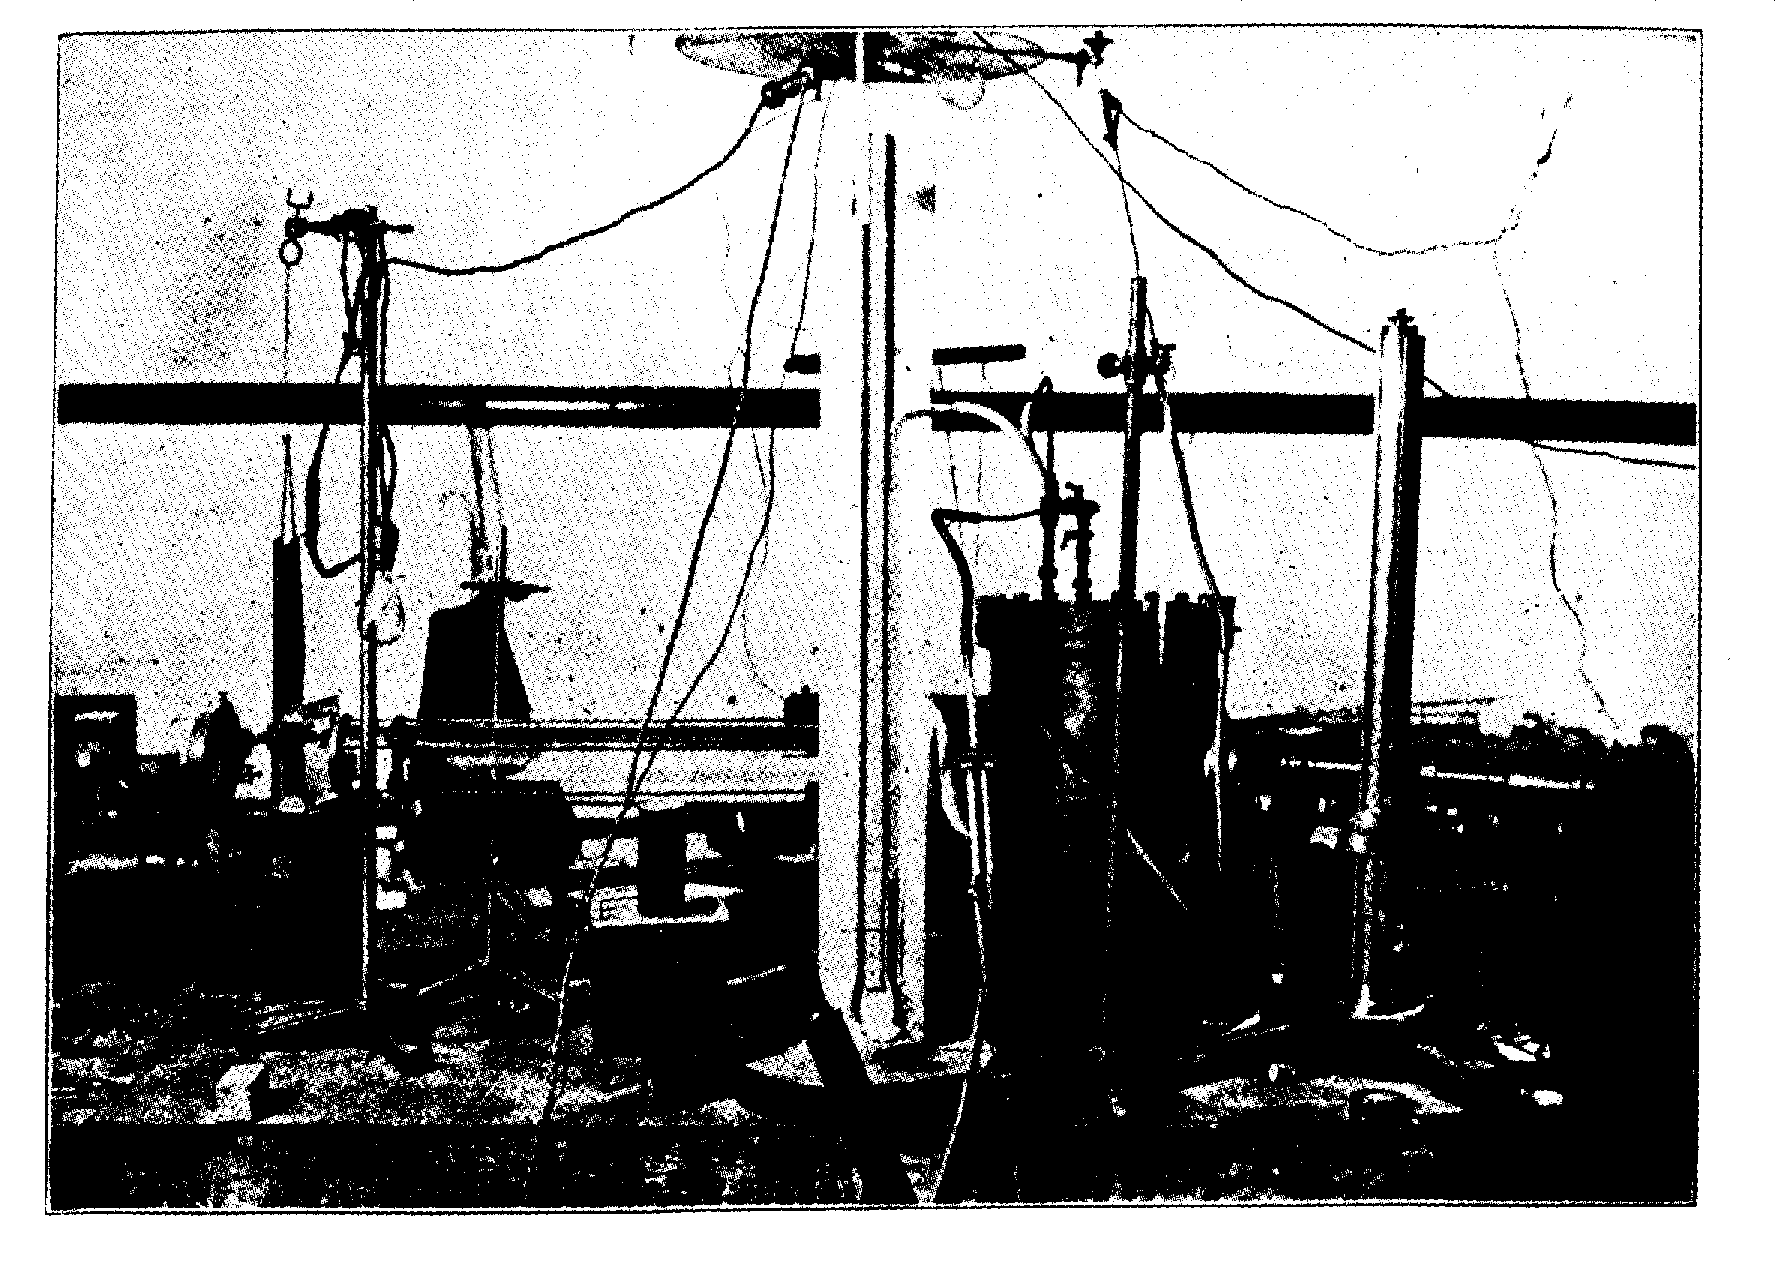
\includegraphics[width=5.91667in,height=4.21667in]{images/00_cover/millikan-apparatus.png}
\end{figure}
\vspace{.5in}
    St. John's College\\ 
    Annapolis, MD
\end{center}
\thispagestyle{empty}
\newpage

\maketitle
\thispagestyle{empty}
\newpage

\vspace*{3in}
Acknowledgements and Notes


\begin{quote}
Selections from R.\ A.\ Millikan reprinted by permission of the University of Chicago Press from \emph{The Electron} by Robert A.\ Millikan, copyright 1917 and 1924 by the University of Chicago.  All rights reserved.  Published 1917.  Second edition 1924.  Tenth impression 1968.  Printed in the United States of America.



The illustration on the cover shows Millikan’s oil-drop apparatus.  This is the design he describes as having achieved “the limit of its possible precision” (\emph{The Electron}, p.\ 115).  

Throughout the manual, explanatory footnotes added to the original texts are indicated by being enclosed in square brackets. Ellipses of up to several sentences are similarly indicated, and longer ellipses by a line with asterisks as below.

\vspace*{11pt}

\centerline{* * *}


\end{quote}
\thispagestyle{empty}
\newpage

\renewcommand{\contentsname}{Table of Contents}
\tableofcontents*

\mainmatter
\pagenumbering{arabic}

\chapter{On the Absolute Quantity of Electricity Associated with the Particles or
Atoms of Matter}

\chapterprecis{}

\chapterprecishere{Michael Faraday\footnote{[\emph{Experimental Researches in Electricity}, 
   VIIth series, section 13. Dover edition, Vol.I, 249ff.]}}
\chapterprecistoc{Michael Faraday}


\makeoddhead{myheadings}{\emph{Faraday}}{}{\thepage}
\makeevenhead{myheadings}{\thepage}{}{\emph{On the Absolute Quantity of Electricity}}

\indent
852. The theory of definite electrolytical or electro-chemical action
appears to me to touch immediately upon the \emph{absolute quantity} of
electricity or electric power belonging to different bodies. It is
impossible, perhaps, to speak on this point without committing oneself
beyond what present facts will sustain; and yet it is equally
impossible, and perhaps would be impolitic, not to reason upon the
subject. Although we know nothing of what an atom is, yet we cannot
resist forming some idea of a small particle, which represents it to the
mind; and though we are in equal, if not greater, ignorance of
electricity, so as to be unable to say whether it is a particular matter
or matters, or mere motion of ordinary matter, or some third kind of
power or agent, yet there is an immensity of facts which justify us in
believing that the atoms of matter are in some way endowed or associated
with electrical powers, to which they owe their most striking qualities,
and amongst them their mutual chemical affinity. As soon as we perceive,
through the teaching of Dalton, that chemical powers are, however varied
the circumstances in which they are exerted, definite for each body, we
learn to estimate the relative degree of force which resides in such
bodies: and when upon that knowledge comes the fact, that the
electricity, which we appear to be capable of loosening from its
habitation for awhile, and conveying from place to place, \emph{whilst
it retains its chemical force}, can be measured out, and being so
measured out is found to be \emph{as definite in its action} as any of
\emph{those portions} which, remaining associated with the particles of
matter, give them their \emph{chemical relation}; we seem to have found
the link which connects the proportion of that we have evolved to the
proportion of that belonging to the particles in their natural state.

853. Now it is wonderful to observe how small a quantity of a compound
body is de\-com\-posed by a certain portion of electricity. Let us, for
instance, consider this and a few other points in relation to water.
\emph{One grain}\footnote{{[}One grain is about .065 grams.{]}} of
water, acidulated to facilitate conduction, will require an electric
current to be continued for three minutes and three quarters of time to
effect its de\-com\-po\-si\-tion, which current must be powerful enough to
retain a platina wire 1/104 of an inch in thickness,\footnote{I have not
  stated the length of wire used, because I find by experiment, as would
  be expected in theory, that it is indifferent. The same quantity of
  electricity which, passed in a given time, can heat an inch of platina
  wire of a certain diameter red hot, can also heat a hundred, a
  thousand, or any length of the same wire to the same degree, provided
  the cooling circumstances are the same for every part in all cases.
  This I have proved by the volta-electrometer. I found that whether
  half an inch or eight inches were retained at one constant temperature
  of dull redness, equal quantities of water were de\-com\-posed in equal
  times. When the half-inch was used, only the center portion of wire
  was ignited. A fine wire may even be used as a rough but ready
  regulator of a voltaic current; for if it be made part of the circuit,
  and the larger wires communicating with it be shifted nearer to or
  further apart, so as to keep the portion of wire in the circuit
  sensibly at the same temperature, the current passing through it will
  be nearly uniform.} red hot, in the air during the whole time; and if
interrupted anywhere by charcoal points, will produce a very brilliant
and constant star of light. If attention be paid to the instantaneous
discharge of electricity of tension, as illustrated in the beautiful
experiments of Mr. Wheatstone,\footnote{Literary Gazette, 1833, March 1
  and 8. Philosophical magazine, 1833, 204. L'Institute, 1833, 261.}
and to what I have said elsewhere on the relation of common and voltaic
electricity (371.\ 375.),\footnote{{[}Faraday refers to numbered
  paragraphs in earlier series of the \emph{Experimental Researches}.{]}}
it will not be too much to say that this necessary quantity of
electricity is equal to a very powerful flash of lightning.\footnote{{[}This
  amount of charge is indeed comparable to that in a typical lightning
  bolt.{]}} Yet we have it under perfect command; can evolve, direct,
and employ it at pleasure; and when it has performed its full work of
electrolyzation, it has only separated the elements of \emph{a single
grain of water.}

854. On the other hand, the relation between the conduction of the
electricity and the de\-com\-po\-si\-tion of the water is so close, that one
cannot take place without the other. If the water is altered only in
that small degree which consists in its having the solid instead of the
fluid state, the conduction is stopped, and the de\-com\-po\-si\-tion is stopped
with it. Whether the conduction be considered as depending upon the
de\-com\-po\-si\-tion, or not (413.\ 703.), still the relation of the two
functions is equally intimate and inseparable.

855. Considering this close and twofold relation, namely, that without
de\-com\-po\-si\-tion transmission of electricity does not occur; and, that for
a given definite quantity of electricity passed, an equally definite and
constant quantity of water or other matter is de\-com\-posed; considering
also that the agent, which is electricity, is simply employed in
overcoming electrical powers in the body subjected to its action; it
seems a probable, and almost a natural consequence, that the quantity
which passes is the \emph{equivalent} of, and therefore equal to, that
of the particles separated; i.e.\ that if the electrical power which
holds the elements of a grain of water in combination, or which makes a
grain of oxygen and hydrogen in the right pro\-por\-tions unite into water
when they are made to combine, could be thrown into the condition of
\emph{a current}, it would exactly equal the current required for the
separation of that grain of water into its elements again.

856. This view of the subject gives an almost overwhelming idea of the
extraordinary quantity or degree of electric power which naturally
belongs to the particles of matter; but it is not inconsistent in the
slightest degree with the facts which can be brought to bear on this
point. To illustrate this I must say a few words on the voltaic
pile.\footnote{By the term voltaic pile, I mean such ap\-pa\-ra\-tus or
  arrangement of metals as up to this time have been called so, and
  which contain water, brine, acids, or other aqueous solutions or
  decomposable substances (476.), between their plates. Other kinds of
  electric ap\-pa\-ra\-tus may hereafter be invented, and I hope to construct
  some not belonging to the class of instruments discovered by Volta.
  {[}Note: The voltaic pile is an instance of what we know as the
  \emph{electric battery}; and indeed Faraday also uses the term
  ``battery'' in paragraphs 858ff. below.{]}}

857. Intending hereafter to apply the results given in this and the
preceding series of Researches to a close investigation of the source of
electricity in the voltaic instrument, I have refrained from forming any
decided opinion on the subject; and without at all meaning to dismiss
metallic contact, or the contact of dissimilar substances, being
conductors, but not metallic, as if they had nothing to do with the
origin of the current, I still am fully of the opinion with Davy, that
it is at least continued by chemical action, and that the supply
constituting the current is almost entirely from that source.

858. Those bodies which, being interposed between the metals of the
voltaic pile, render it active, \emph{are all of them electrolytes}
(476.); and it cannot but press upon the attention of every one engaged
in considering this subject, that in those bodies (so essential to the
pile) de\-com\-po\-si\-tion and the transmission of a current are so intimately
connected, that one cannot happen without the other. This I have shown
abundantly in water, and in numerous other cases (402.\ 476.). If, then,
a voltaic trough have its extremities connected by a body capable of
being de\-com\-posed, as water, we shall have a continuous current through
the ap\-pa\-ra\-tus; and whilst it remains in this state we may look at the
part where the acid is acting upon the plates, and that where current is
acting upon the water, as the reciprocals of each other. In both parts
we have the two conditions \emph{inseparable in such bodies as these},
namely, the passing of a current, and de\-com\-po\-si\-tion; and this is as true
of the cells in the battery as of the water cell; for no voltaic battery
has as yet been constructed in which the chemical action is only that of
combination: \emph{de\-com\-po\-si\-tion is always included}, and is, I believe,
an essential chemical part.

859. But the difference in the two parts of the connected battery, that
is, the de\-com\-po\-si\-tion or experimental cell, and the acting cells, is
simply this. In the former we urge the current through, but it,
apparently of necessity, is accompanied by de\-com\-po\-si\-tion: in the latter
we cause de\-com\-po\-si\-tions by ordinary chemical actions (which are,
however, themselves electrical), and, as a consequence, have the
electrical current; and as the de\-com\-po\-si\-tion dependent upon the current
is definite in the former case, so is the current associated with the
de\-com\-po\-si\-tion also definite in the latter (862.\ \&c.).

860. Let us apply this in support of what I have surmised respecting the
enormous electric power of each particle or atom of matter (856.). I
showed in a former series of these Researches on the relation by measure
of common and voltaic electricity,\footnote{{[}By ``common'' electricity
  Faraday means \emph{static} electricity; while ``voltaic'' electricity
  is what is produced by the voltaic battery. Until Faraday showed their
  equivalence, it was uncertain whether the two ``electricities'' were
  same or different.{]}} that two wires, one of platina and one of zinc,
each one eighteenth of an inch in diameter, placed five-sixteenths of an
inch apart, and immersed to the depth of five eighths of an inch in
acid, consisting of one drop of oil of vitriol and four ounces of
distilled water at a temperature of about $60^{\circ}$ Fahr., and connected at
the other extremities by a copper wire eighteen feet long, and one
eighteenth of an inch in thickness,\footnote{{[}The eighteen-foot length
  of wire formed the coil of a galvanometer. See \emph{Experimental
  Researches}, Vol. I, 105.{]}} yielded as much electricity in little
more than three seconds of time as a Leyden battery\footnote{{[}``Leyden
  battery'': an array (a ``battery'') of Leyden jars.{]}} charged by
thirty turns of a very large and powerful plate electric machine in full
action (371.). This quantity, though sufficient if passed through the
head of a rat or cat to have killed it, as by a flash of lightning, was
evolved by the mutual action of so small a portion of the zinc wire and
water in contact with it, that the loss of weight sustained by either
would be inappreciable by our most delicate instruments; and as to the
water which could be de\-com\-posed by that current, it must have been
insensible in quantity, for no trace of hydrogen appeared upon the
surface of the platina during those three seconds.

861. What an enormous quantity of electricity, therefore, is required
for the de\-com\-po\-si\-tion of a single grain of water! We have already seen
that it must be in quantity sufficient to sustain a platina wire 1/104
of an inch in thickness, red hot, in contact with the air, for three
minutes and three quarters (853.), a quantity which is almost infinitely
greater than that which could be evolved by the little standard voltaic
arrangement to which I have just referred (860.\ 371.). I have endeavored
to make a comparison by the loss of weight of such a wire in a given
time in such an acid, according to a principle and experiment to be
almost immediately described (862.); but the proportion is so high that
I am almost afraid to mention it. It would appear that 800,000 such
charges of the Leyden battery as I have referred to above, would be
necessary to supply electricity sufficient to decompose a single grain
of water; or, if I am right, to equal the quantity of electricity which
is naturally associated with the elements of that grain of water,
endowing them with their mutual chemical affinity.

862. In further proof of this high electric condition of the particles
of matter, and the \emph{identity as to quantity of that belonging to
them with that necessary for their separation}, I will describe an
experiment of great simplicity but extreme beauty, when viewed in
relation to the evolution of an electric current and its decomposing
powers.

863. A dilute sulphuric acid, made by adding about one part by measure
of oil of vitriol to thirty parts of water, will act energetically upon
a piece of zinc plate in its ordinary and simple state: but, as Mr.
Sturgeon has shewn,\footnote{Recent Experimental Researches, \&c., 1830,
  74, \&c.} not at all, or scarcely so, if the surface of the metal
has in the first instance been amalgamated; yet the amalgamated zinc
will act powerfully with platina as an electromotor,\footnote{{[}``electromotor'':
  something that moves or tends to move electricity (1827).{]}} hydrogen
being evolved on the surface of the latter metal, as the zinc is
oxidized and dissolved. The amalgamation is best effected by sprinkling
a few drops of mercury upon the surface of the zinc, the latter being
moistened with the dilute acid, and rubbing with the fingers or tow so
as to extend the liquid metal over the whole of the surface. Any mercury
in excess, forming liquid drops upon the zinc, should be wiped
off.\footnote{The experiment may be made with pure zinc, which, as
  chemists well know, is but slightly acted upon by dilute sulphuric
  acid in comparison with ordinary zinc, which during the action is
  subject to an infinity of voltaic actions. See De la Rive on this
  subject, Bibliothèque Universelle, 1830, 391.}

864. Two plates of zinc thus amalgamated were dried and accurately
weighed; one, which we shall call A, weighed 163.1 grains; the other, to
be called B, weighed 148.3 grains.\footnote{{[}Or, since one grain
  equals about .065 grams, plate A weighs about 10.6 grams and plate B
  about 9.6 grams.{]}} They were about five inches long, and 0.4 of an
inch wide. An earthenware pneumatic trough was filled with dilute
sulphuric acid, of the strength just described (863.), and a gas jar,
also filled with the acid, inverted in it.\footnote{The acid was left
  during a night with a small piece of unamalgamated zinc in it, for the
  purpose of evolving such air as might be inclined to separate, and
  bringing the whole into a constant state.} A plate of platina of
nearly the same length, but about three times as wide as the zinc
plates, was put up into this jar. The zinc plate A was also introduced
into the jar, and brought in contact with the platina, and at the same
moment the plate B was put into the acid of the trough, but out of
contact with other metallic matter.

865. Strong action immediately occurred in the jar upon the contact of
the zinc and platina plates. Hydrogen gas rose from the platina, and was
collected in the jar, but no hydrogen or other gas rose from
\emph{either} zinc plate. In about ten or twelve minutes, sufficient
hydrogen having been collected, the experiment was stopped; during its
progress a few small bubbles had appeared upon plate B, but none upon
plate A. The plates were washed in distilled water, dried, and
reweighed. Plate B weighed 148.3 grains, as before, having lost nothing
by the direct chemical action of the acid. Plate A weighed 154.65
grains, 8.45 grains of it having been oxidized and dissolved during the
experiment.

\begin{figure}
  \begin{center}
    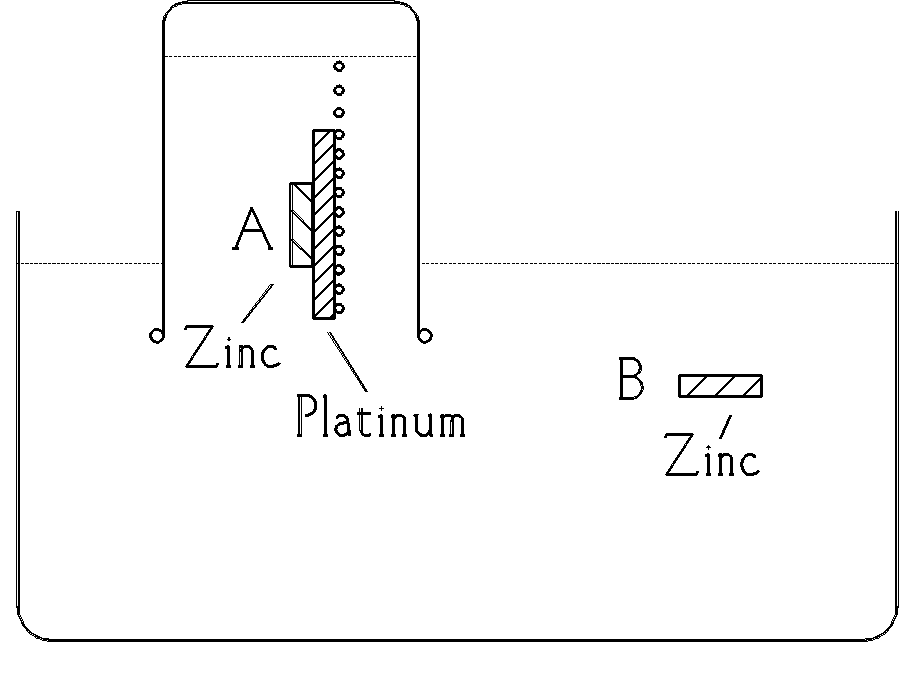
\includegraphics[width=2.68681in,height=2.00903in]{images/01_faraday/image001.png}
    \caption*{{[}A representation of Faraday's ap\-pa\-ra\-tus.{]}}
  \end{center}
\end{figure}

866. The hydrogen gas was next transferred to a water-trough and
measured; it amounted to 12.5 cubic inches, the temperature being $52^{\circ}$,
and the barometer 29.2 inches. This quantity, corrected for temperature,
pressure, and moisture, becomes 12.15453 cubic inches of dry hydrogen at
mean temperature and pressure;\footnote{{[}Faraday uses the gas laws to
  reduce the measured volume of hydrogen to the equivalent volume at $50^{\circ}$
  F. and 30 in Hg; these are ``mean'' conditions which he takes as
  standard. The measurement is first ``corrected for moisture'' by
  subtracting the known vapor pressure of water at $52^{\circ}$ F. from the
  measured barometric pressure.{]}} which, increased by one half for the
oxygen that must have gone to the \emph{anode}, i.e.\ to the zinc, gives
18.232 cubic inches as the quantity of oxygen and hydrogen evolved from
the water de\-com\-posed by the electric current.\footnote{{[}Since
  de\-com\-po\-si\-tion of water yields hydrogen and oxygen in a 2:1 ratio by
  volume, the total volume of both gases will be 1.5 times the volume of
  hydrogen alone.{]}} According to the estimate of the weight of the
mixed gas before adopted (791.),\footnote{{[}In an earlier paragraph
  791, Faraday had reported about .129 grains per cubic inch as the
  density of a mixture of 2 volumes hydrogen and 1 volume oxygen at
  ``mean'' temperature and pressure.{]}} this volume is equal to
2.3535544 grains, which therefore is the weight of water de\-com\-posed; and
this quantity is to 8.45 {[}grains{]}, the quantity of zinc oxidized, as
9 is to 32.31. Now taking 9 as the equivalent number of water, the
number 32.5 is given as the equivalent number of zinc;\footnote{{[}The
  equivalent weight of zinc currently accepted is 32.69, about .5\%
  higher than the figure 32.5 accepted by Faraday.{]}} a coincidence
sufficiently near to show, what indeed could not but happen, that for an
equivalent of zinc oxidized an equivalent of water must be
de\-com\-posed.\footnote{The experiment was repeated several times with the
  same results.}

867. But let us observe \emph{how} the water is de\-com\-posed. It is
electrolyzed, i.e.\ is de\-com\-posed voltaically, and not in the ordinary
manner (as to appearance) of chemical de\-com\-po\-si\-tions; for the oxygen
appears at the \emph{anode} and the hydrogen at the \emph{cathode} of
the body under de\-com\-po\-si\-tion, and these were in many parts of the
experiment above an inch asunder. Again, the ordinary chemical affinity
was not enough under the circumstances to effect the de\-com\-po\-si\-tion of
the water, as was abundantly proved by the inaction on plate B; the
voltaic current was essential. And to prevent any idea that the chemical
affinity was almost sufficient to decompose the water, and that a
smaller current of electricity might, under the circumstances, cause the
hydrogen to pass to the \emph{cathode}, I need only refer to the results
which I have given (807.\ 813.), to shew that the chemical action at the
electrodes has not the slightest influence over the \emph{quantities} of
water or other substances de\-com\-posed between them, but that they are
entirely dependent upon the quantity of electricity which passes.

868. What, then, follows as a necessary consequence of the whole
experiment? Why, this: that the chemical action upon 32.31 parts, or one
equivalent of zinc, in this simple voltaic circle, was able to evolve
such quantity of electricity in the form of a current as, passing
through water, should decompose 9 parts, or one equivalent of that
substance: and considering the definite relations of electricity as
developed in the preceding parts of the present paper, the results prove
that the quantity of electricity which, being naturally associated with
the particles of matter, gives them their combining power, is able, when
thrown into a current, to separate those particles from their state of
combination; or, in other words, that \emph{the electricity which
decomposes, and that which is evolved by the de\-com\-po\-si\-tion of, a certain
quantity of matter, are alike}.

869. The harmony which this theory of the definite evolution and the
equivalent definite action of electricity introduces into the associated
theories of definite pro\-por\-tions and electro-chemical affinity, is very
great. According to it, the equivalent weights of bodies are simply
those quantities of them which contain equal quantities of electricity,
or have naturally equal electric powers; it being the
\textsc{electricity} which \emph{determines} the equivalent number,
\emph{because} it determines the combining force. Or, if we adopt the
atomic theory or phraseology, then the atoms of bodies which are
equivalent to each other in their ordinary chemical action, have equal
quantities of electricity naturally associated with them. But I must
confess I am jealous\footnote{{[}``jealous:'' here,
  \emph{suspicious}.{]}} of the term \emph{atom}; for though it is very
easy to talk of atoms, it is very difficult to form a clear idea of
their nature, especially when compound bodies are under consideration.

870. I cannot refrain from recalling here the beautiful idea put forth,
I believe, by Berzelius (703.)\ in his development of his views of the
electro-chemical theory of affinity, that the heat and light evolved
during cases of powerful combination are the consequence of the electric
discharge which is at the moment taking place. The idea is in perfect
accordance with the view I have taken of the \emph{quantity} of
electricity associated with the particles of matter.

871. In this exposition of the law of the definite action of
electricity, and its cor\-re\-spond\-ing definite proportion in the particles
of bodies, I do not pretend to have brought, as yet, every case of
chemical or electro-chemical action under its dominion. There are
numerous considerations of a theoretical nature, especially respecting
the compound particles of matter and the resulting electrical forces
which they ought to possess, which I hope will gradually receive their
development; and there are numerous experimental cases, as, for
instance, those of compounds formed by weak affinities, the simultaneous
de\-com\-po\-si\-tion of water and salts, \&c., which still require
investigation. But whatever the results on these and numerous other
points may be, I do not believe that the facts which I have advanced, or
even the general laws deduced from them, will suffer any serious change;
and they are of sufficient importance to justify their publication,
though much may yet remain imperfect or undone. Indeed, it is the great
beauty of our science, \textsc{chemistry}, that advancement in it,
whether in a degree great or small, instead of exhausting the subjects
of research, opens the doors to further and more abundant knowledge,
overflowing with beauty and utility, to those who will be at the easy
personal pains of undertaking its experimental investigation.

872. The definite production of electricity (868.)\ in association with
its definite action proves, I think, that the current of electricity in
the voltaic pile is sustained by chemical de\-com\-po\-si\-tion, or rather by
chemical action, and not by contact only. But here, as elsewhere (857.),
I beg to reserve my opinion as to the real action of contact, not having
yet been able to make up my mind as to whether it is an exciting cause
of the current, or merely necessary to allow of the conduction of
electricity, otherwise generated, from one metal to the other.

873. But admitting that chemical action is the source of electricity,
what an infinitely small fraction of that which is active do we employ
in our voltaic batteries! Zinc and platina wires, one eighteenth of an
inch in diameter and about half an inch long, dipped into dilute
sulphuric acid, so weak that it is not sensibly sour to the tongue, or
scarcely to our most delicate test papers, will evolve more electricity
in one twentieth of a minute (860.)\ than any man would willingly allow
to pass through his body at once. The chemical action of a grain of
water upon four grains of zinc can evolve electricity equal in quantity
to that of a powerful thunder-storm (868.\ 861.). Nor is it merely true
that the quantity is active; it can be directed and made to perform its
full equivalent duty (867.\ \&c.). Is there not, then, great reason to
hope and believe that, by a closer \emph{experimental} investigation of
the principles which govern the development and action of this subtile
agent, we shall be able to increase the power of our batteries, or
invent new instruments which shall a thousandfold surpass in energy
those which we at present possess?

874. Here for a while I must leave the consideration of the
\emph{definite chemical action of electricity}. But before I dismiss
this series of experimental Researches, I would call to mind that, in a
former series, I showed the current of electricity was also
\emph{definite in its magnetic action} (216.\ 366.\ 367.\ 376.\ 377.); and,
though this result was not pursued to any extent, I have no doubt that
the success which has attended the development of the chemical effects
is not more than would accompany an investigation of the magnetic
phenomena.

\begin{quotation}
\emph{Royal Institution}

\emph{December} 31\emph{st}, 1833.
\end{quotation}

\section*{A Note on Chemical Equivalence}

Faraday confesses he is ``jealous,'' that is, suspicious, of the term
\emph{atom}. When he wrote in 1833, there was no agreement among natural
philosophers as to a formula for, say, water, which would specify the
atomic constituents of a single smallest particle (mol\-e\-cule) of water:
was it HO, or H$_2$O, or something else? What Faraday \emph{was} sure of
was that chemical substances reacted in definite pro\-por\-tions by weight
and, further, that the weights of various substances reacting with one
another formed a series of ``equivalent'' or ``combining'' weights. And
since oxygen combines with so many different substances, taking oxygen
as the standard of comparison allowed indirect extension of the series
to include \emph{all} elements.

For example, 8 parts by weight of oxygen will combine with 1 part by
weight of hydrogen (to form water). But 8 parts by weight of oxygen will
also combine with 32.69 parts by weight of zinc (to form zinc oxide).
Then the 32.69 of zinc, the 8 of oxygen, and the 1 of hydrogen are all
said to be ``equivalent'' weights---equivalent, that is to say, in
\emph{combining power---}because either any two of those quantities will
combine with one another or each will combine with the specified weight
of the remaining substance. Equivalent weights are relative only to one
another and may therefore be expressed in arbitrary units of weight. But
it is particularly convenient to express them in \emph{grams}, with
\emph{8 grams of oxygen} taken as the standard. The figures so obtained
are called, not merely equivalent weights, but \emph{gram-equivalent
weights}; thus 1 gram, 8 grams, and 32.69 grams are the
\emph{gram-equivalent weights} of hydrogen, oxygen, and zinc,
respectively.

If, like Faraday, one is skeptical of the atomic view, there cannot be
assumed any natural ``unit'' of chemical combining power. Thus it is for
him illuminating in the highest degree to be able to interpret the
chemically equivalent weights of various substances as amounts which
contain ``equal quantities of electricity'' (cf.\ his paragraph 869
above).

If the atomic view is accepted, there are consequences even more
far-reaching. The molecular formulas finally propounded by Cannizzaro
(\emph{A Course in Chemical Philosophy}, 1859) show that one atom of an
element may hold in combination one, two or more atoms of other elements
by establishing an integral number of \emph{atomic bonds}, where the
bond to a hydrogen atom is taken as unit.\footnote{The number of bonds
  an atom has formed is known as its \emph{valence}. Thus in H2O (water)
  and NH3 (ammonia), the oxygen atom is said to be \emph{bivalent} and
  the nitrogen atom \emph{tervalent}. Some elements combine under
  different conditions to form more than one compound, allowing a single
  element to exhibit multiple valences. For example, a carbon atom is
  bivalent in CO but quadrivalent in CO2.

  Since ``equivalent weights'' of elements are amounts which display the
  same combining power, then on the atomic view they must also be
  amounts that form the same total number of atomic bonds. But any
  number of bivalent atoms will form as many bonds as \emph{twice} that
  number of univalent atoms; and in general, equivalent weights of
  different elements must contain numbers of atoms inversely
  proportional to their respective valences. Therefore we may state that
  \emph{the relative weights of the atoms} of different elements are as
  \emph{the products of their equivalent weights times their valences},
  respectively; or:

  Atomic weight = Equivalent weight $\times$ Valence.} Since, on the atomic
view, an atom that forms a single atomic bond manifests \emph{a natural
unit of combining power,} then under Faraday's interpretation of chemical
powers as ultimately electrical, such a unitary combining power would
appear to be associated with and perhaps even explained by \emph{a
natural unit of electricity.}

Might there really be a natural unit of electricity, an ``atom of
charge''? The papers to follow by Thomson and Millikan will bear on this
question.

\section*{Experiment: Electrodeposition of Copper}

In order to simplify the relations between chemical and electrical power
in our ap\-pa\-ra\-tus, we use a cell in which no overall chemical reaction
occurs. This is achieved by using electrodes made of the same metal as
the metal in the electrolytic solution. Under the action of electric
current metal from the positive electrode (anode) dissolves into
solution, while at the negative electrode (cathode) metal leaves the
solution and is deposited there. The net result is transfer of material
from one electrode to the other. We normally use copper electrodes, with
a copper sulfate solution as electrolyte. If available, silver
electrodes with a silver nitrate solution can be employed for comparison
with another element.\footnote{The experiment can easily be done with
  silver, provided the silver nitrate solution is protected from light;
  however the supplies are much more expensive and harder to recover
  after use.}

You may choose to weigh either the cathode, which gains material, or the
anode, which loses it. It is theoretically advantageous to weigh the
\emph{cathode}, since the anode is subject to secondary reactions in the
presence of an acid solution, producing excessive weight loss. On the
other hand, material removed from the anode may fail to adhere to the
cathode, resulting in deficient measurement of the weight gain.
Whichever your choice, results will be greatly improved if you
\emph{start with clean electrodes} and \emph{avoid excessive currents}.

The electrolyte solution is cupric sulfate dissolved in distilled water,
with the ad\-di\-tion of a small quantity of sulfuric acid, which enhances
the conductivity of the solution.

Power is furnished by a standard supply. A rheostat of about 20 ohms is
used to help regulate the current. Typically 1-2 amperes is the current
used. Higher values will require constant readjustment of the rheostat
and may cause de\-com\-po\-si\-tion of the water, as well as other problems.

\begin{figure}
\begin{center}
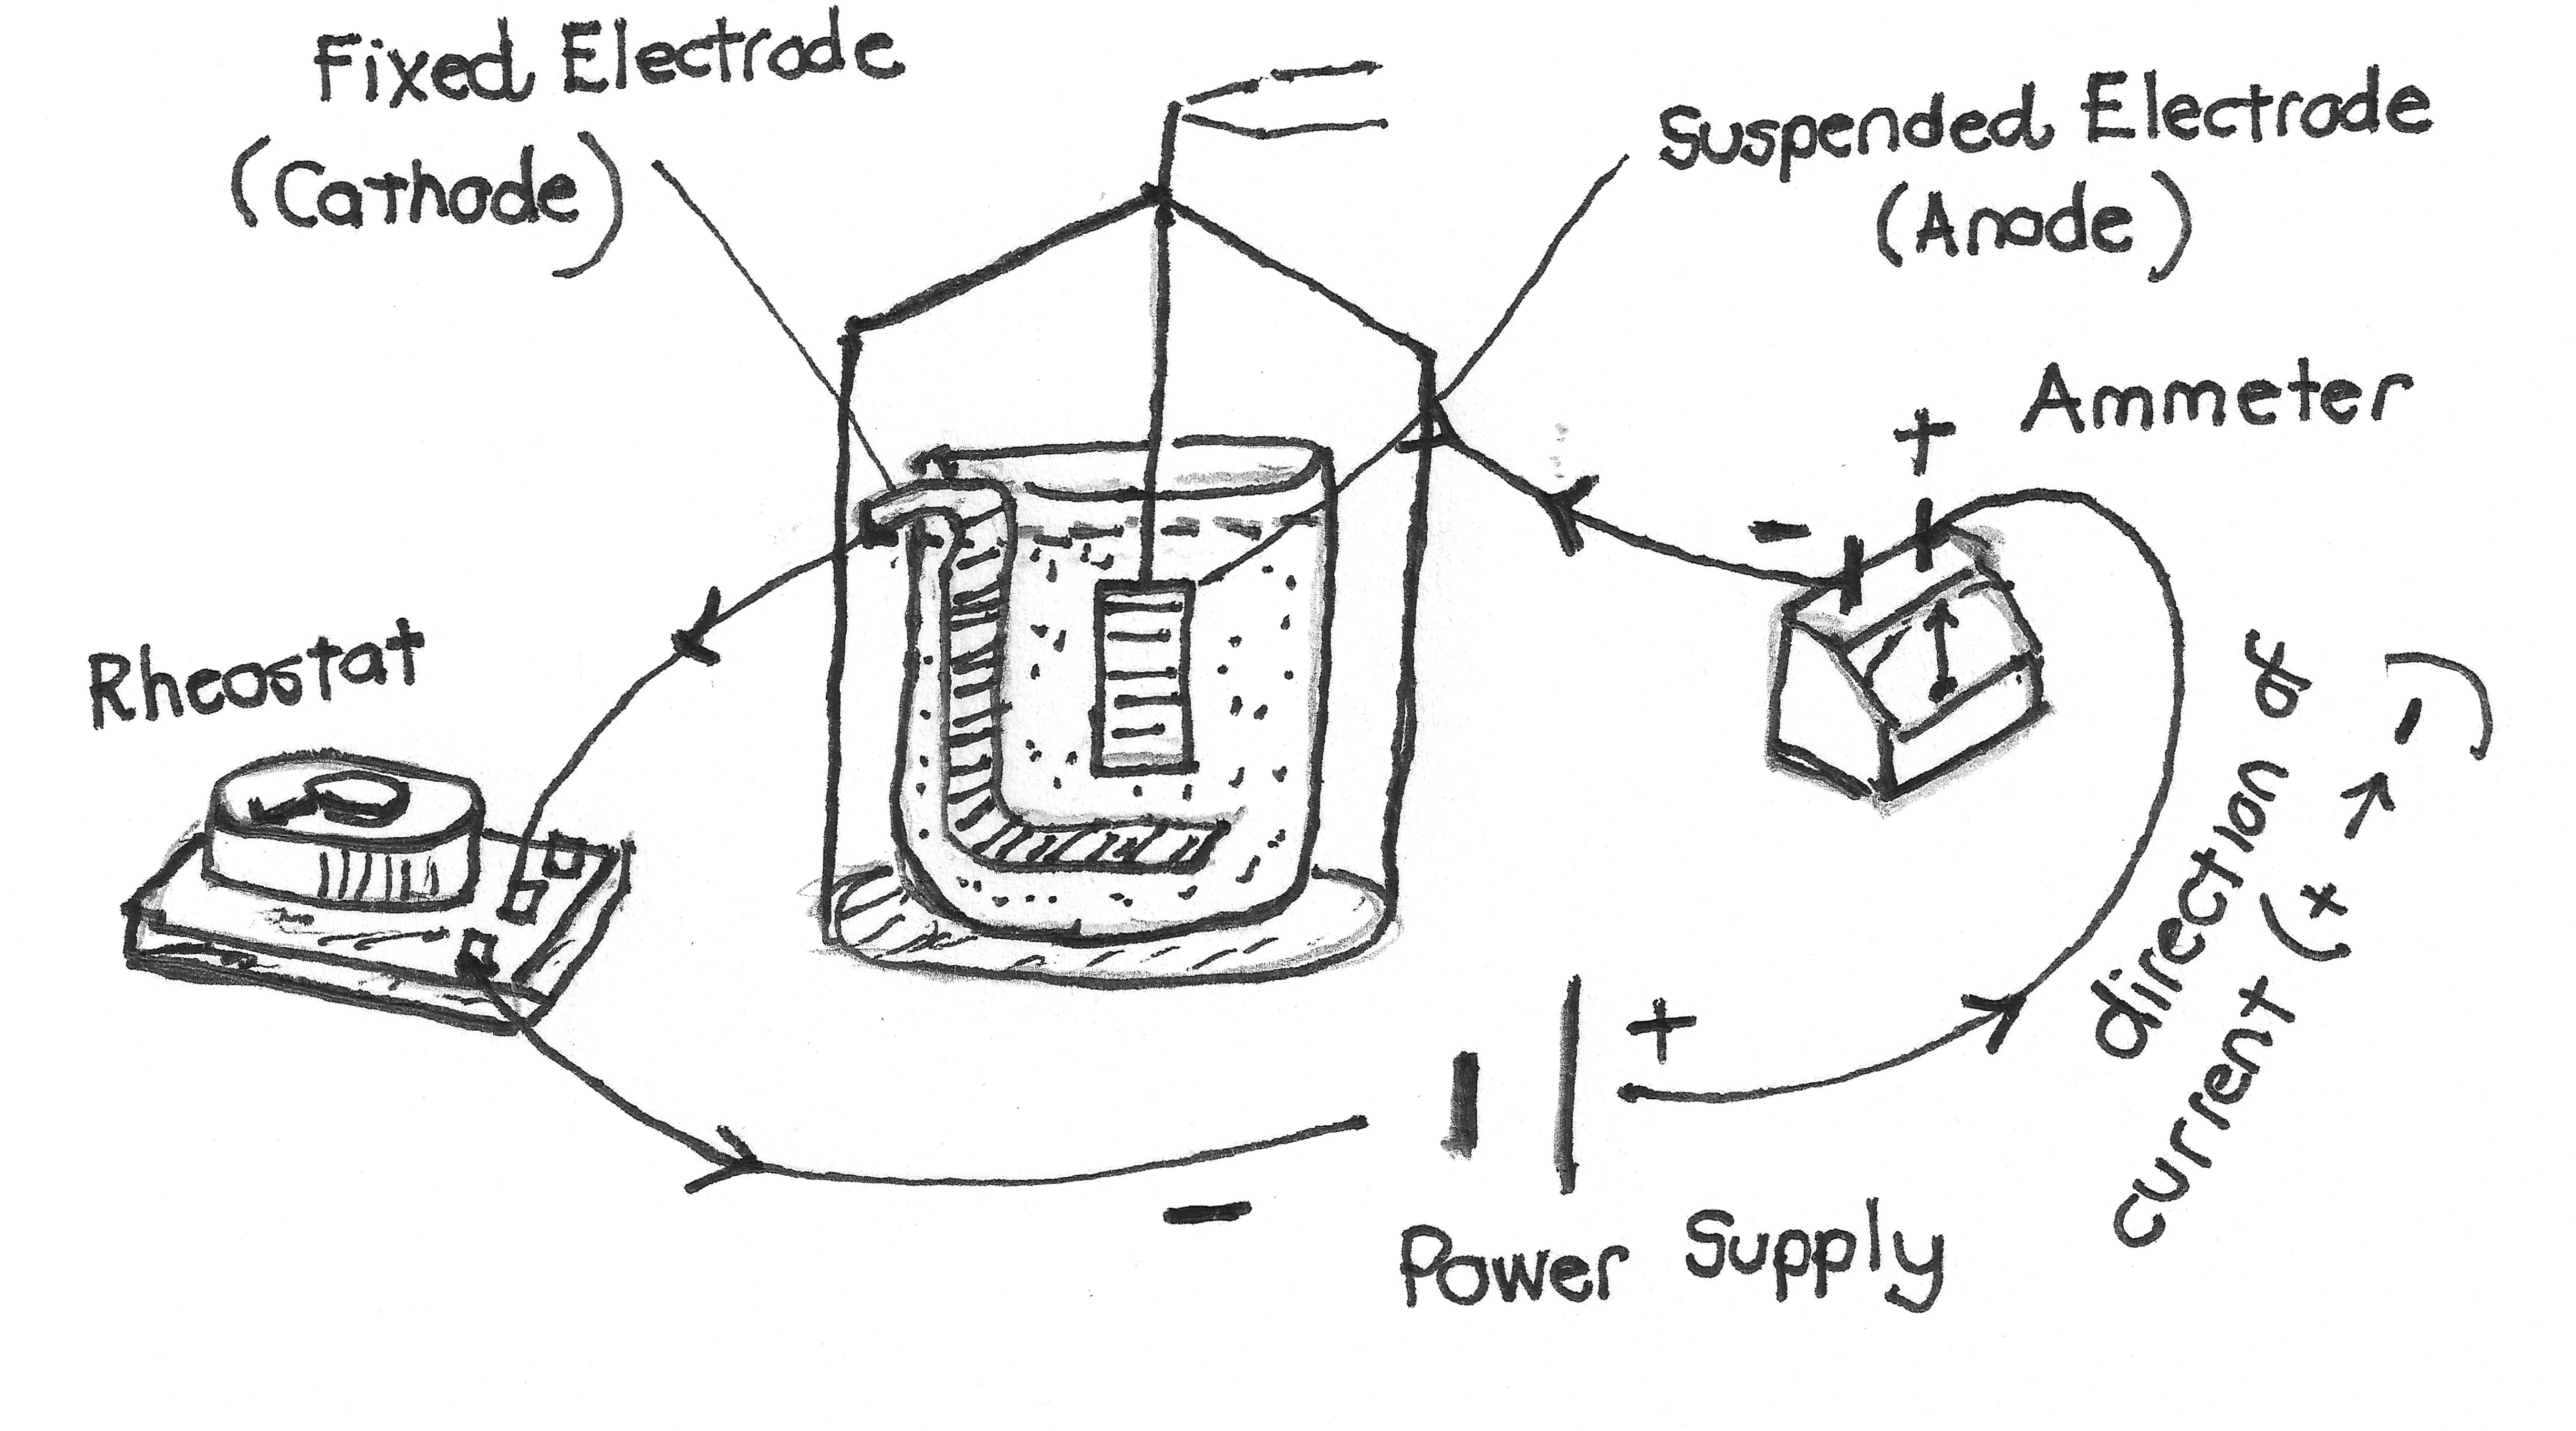
\includegraphics[width=4.88403in,height=2.20694in]{images/01_faraday/image003.png}
\caption*{\emph{With this wiring, the suspended copper electrode is an anode; the
fixed copper electrode a cathode. Copper is lost at the anode and gained at the cathode.
To reverse anode and cathode, run the current from the power
supply in the reverse directions, remembering that current in the
ammeter runs from positive (terminal) to negative.}}
\end{center}
\end{figure}

The plate to be weighed will be suspended directly from a metal stand.
The beaker, containing the electrolyte solution and the fixed electrode,
rests on the workbench. The fixed electrode is cut from a strip of pure
copper sheet and is about 1 inch wide; it must be long enough to run
along the bottom of the beaker.\footnote{This is to establish an
  electric field on both sides of the suspended plate; otherwise the
  action may be slow or erratic.} It should be bent to fit the edge of
the beaker and guided far enough away from the suspended plate to
prevent accidental contact.

Weigh both plates on the electronic balance. Then fit the fixed plate
into the beaker, and adjust the length of the suspension hook so that
the suspended plate can swing freely without touching the fixed plate.
You will have to make at least two plating trials.

Some groups will attach the spring clips---as suggested in the 
sketch---others will reverse them. Attach the fixed plate to the desired pole of
the power supply.

Next clip the remaining power supply lead to the fixed electrode. Start
a stopwatch as you turn on the power supply, and quickly bring the
current to some value between 1 and 2 amperes.\footnote{Don't waste time
  trying to target a "round number." In this age of pocket calculators,
  round numbers carry no advantage whatever. It is not important that
  the current have any particular value, but that it be \emph{steady}.}
During the run, continually adjust the rheostat to maintain a uniform
current through the solution.\footnote{Note that our rheostat
  illustrates the very technique Faraday mentioned in his note 3 
  above for using a fine (and hence high-resistance) wire as a current
  regulator!} In order to transfer an amount of material that will be
large compared with the sensitivity of the balance, it is best to plate
for at least 20 minutes if a 1-ampere current is used, at least 10
minutes if a 2-ampere current is used. Longer times give greater
precision of measurement, since the weights of material transferred are
then larger in relation to the uncertainty of the weight mea\-sure\-ments.

At the conclusion of the first timed run, turn off the power and remove
the beam clip and the electrical connection to the pan. Gently remove
the suspended electrode and dry it with a hair dryer before measuring
its change in weight.

Carry out a second run similar to the first. It is not necessary to keep
either the current or the plating time the same as before.

We are now in a position to investigate two relations which Faraday
observed to hold in electrolysis:

\subsection{Proportionality Between Weight and Charge for a Single Element}

According to Faraday, the quantity of charge that is supplied to an
electrochemical reaction during any time will be directly proportional
to the quantity of material de\-com\-posed (or transferred) in that time. We
first attempt to exhibit that proportionality.

Calculate the \emph{weight} of material transferred to or from the
weighing plate during the first run, and cumulatively over both runs.

Calculate the quantity of \emph{charge} passed during the first run, and
cumulatively over both runs:

\begin{equation*}
\text{Charge in coulombs = uniform current in amperes $\times$ time in seconds}
\end{equation*}

If the expected proportionality holds, the weight of material
transferred during the first run will be to the total weight transferred
as the charge calculated for the first plating is to the total charge
passed. Do the weights have to one another the same ratio as the
calculated charges?

\subsection{The Ratio of Charge to Weight for Multiple Elements}

We have, it is hoped, observed in electrolysis a constant relation
between charge and weight for a single element. But as Faraday also
described, the weights of two or more elements liberated or transferred
by the same quantity of charge are to one another in the same ratio as
their \emph{chemically equivalent weights}. Or, differently expressed,
\emph{the ratio between charge and equivalent weight is the same for all
elements.}

Faraday recognized this constant proportion, but he could not express it
in terms of a conventional unit of charge since at that time no such
standard had been defined.\footnote{Hence his recourse to such
  expressions as: ``sufficient to keep a platinum wire red hot,'' ``more
  than any man would willingly allow to pass through his body at once,''
  ``thirty turns of a very large and powerful plate machine.''} Using a
modern unit, it has subsequently been determined that a charge of about
96,500 coulombs\footnote{See the Appendix (p.~\pageref{ch:appendix})
for information about the various systems of measurement of electrical quantities.} 
is required to liberate one gram-equivalent weight of any element. That
quantity, 96,500 C, was named the \emph{faraday} in that
investigator's honor. The mea\-sure\-ments we have already taken in
electrodeposition of copper will permit us to calculate the faraday for
ourselves.

For we found in that experiment that a charge $Q$ was required to
transfer $\Delta W$ of copper. Now 1 faraday, $F$, is the charge
required to transfer one gram-equivalent weight of copper---31.78 g.
But the charges are to one another as the weights, as presumably we have
just confirmed; therefore

\begin{equation*}
Q : F :: \Delta W : 31.78\; \text{grams}.
\end{equation*}

Or, expressed algebraically,
\begin{equation*}
F = \frac{31.78\cdot Q}{\Delta W}.
\end{equation*}

Thus the faraday will equal the product of the charge passed in any run
of the electrodeposition experiment, times the gram-equivalent weight of
copper, divided by the weight of copper deposited in that run.

As we shall see, the actual size of the faraday---that is, the quantity
of charge found to be associated with one gram-equivalent weight of an
element in electrolysis---will become pivotal in some speculations which
J.\ J.\ Thomson allows himself in his paper that follows.

(It is, as Faraday himself keenly appreciated, extremely large: two
one-faraday charges placed one kilometer apart---if it were possible to do
this---would e\-lec\-tro\-stat\-ic\-al\-ly attract each other with a force of
\emph{trillions} of pounds.)

\chapter{Cathode Rays}

\chapterprecis{J.\ J.\ Thomson}

\makeoddhead{myheadings}{\emph{Thomson}}{}{\thepage}
\makeevenhead{myheadings}{\thepage}{}{\emph{Cathode Rays}}

\renewcommand{\theequation}{\arabic{equation}}

\section*{Remarks}

\begin{wrapfigure}[8]{r}{0.33\textwidth}
  \begin{center}
    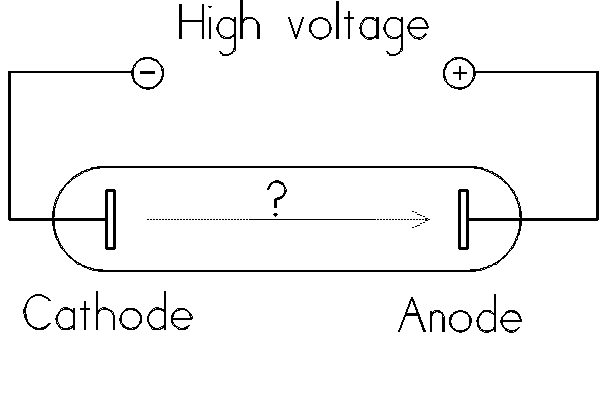
\includegraphics[width=2in,height=1.26042in]{images/02_thomson/image001.png}
  \end{center}
\end{wrapfigure}

\indent

We pursue
further the investigation of ``charge,'' particularly its relation to
matter. An avenue for investigation of this question was opened by the
discovery of the so-called ``cathode rays.'' If a glass tube into which
two electrodes had been sealed was evacuated, and if a high potential
difference was placed across the two electrodes, a mysterious emanation
issued from the cathode (negative electrode), evidenced, among other
manifestations, by its ability to cause phosphors and even certain types
of glass to \emph{glow}. These rays, like the ionic motions in
electrolysis, served to complete the circuit and thus in a sense to
``separate the current from the wire'' and make it available for
independent study. J.\ J.\ Thomson, making the initial hypothesis that the
rays consisted of a flow of electrified particles, showed that they did
indeed exhibit properties of both mass and charge, related in a definite
manner.
\begin{wrapfigure}[8]{l}{0.33\textwidth}
  \begin{center}
    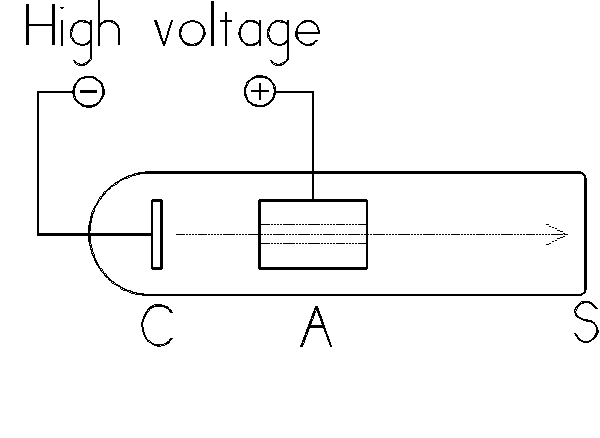
\includegraphics[width=2in,height=1.26042in]{images/02_thomson/image003.png}
  \end{center}
\end{wrapfigure}

Thomson's
1897 paper on cathode rays is reproduced in part below. He assumes the
reader to be familiar with the cathode ray phenomenon. We have sketched
two forms of the cathode-ray apparatus here. First depicted is the
simplest version: C is the cathode and A the anode of an evacuated tube.
The anode contains a small slit; and that a ray of some sort passes
through the slit is shown by a bright spot on the zinc sulfide screen S.
The spot (and hence the ``ray'') can be deflected by bringing a magnet
near the tube in the region between A and S.


\begin{wrapfigure}[8]{r}{0.33\textwidth}
  \begin{center}
    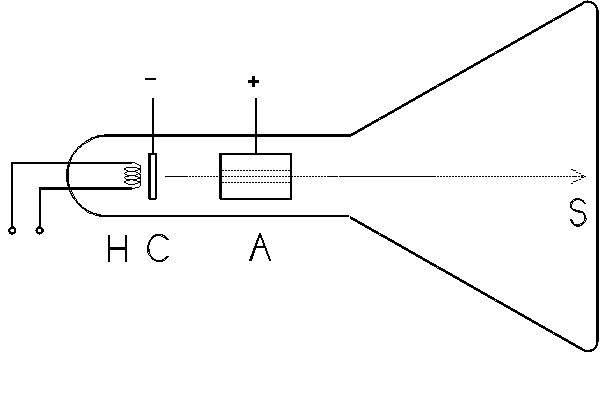
\includegraphics[width=2in,height=1.25in]{images/02_thomson/image005.png} 
  \end{center}
\end{wrapfigure}
The next sketch shows a modern form of cathode-ray tube, much like an
oscilloscope or television picture tube. Here H is an
electrically-heated wire mounted close to cathode C, for it is found
that production of rays is greatly increased if the cathode is heated.
One cylindrical anode A is drawn in the figure, but in practice
additional anodes are sometimes used to bring the beam to a sharp focus
on screen S. The beam may be deflected magnetically or, as Thomson
shows, electrostatically. It becomes then a delicate and versatile
pencil capable of drawing patterns on the screen which faithfully
reflect conditions in the circuits governing the electric or magnetic
deflection.


\section*{Cathode Rays\footnote{{[}\emph{Philosophical Magazine}, \textbf{44}
 (1897), 293--311.{]}}\\ {\large J.\ J.\ Thomson}}


The experiments discussed in this paper were undertaken in the hope of
gaining some information as to the nature of the Cathode Rays. The most
diverse opinions are held as to these rays; according to the almost
unanimous opinion of German physicists they are due to some process in
the æther to which---inasmuch as in a uniform magnetic field their
course is circular and not linear---no phenomenon hitherto observed is
analogous: another view of these rays is that, so far from being wholly
ætherial, they are in fact wholly material, and that they mark the paths
of particles of matter charged with negative electricity. It would seem
at first sight that it ought not to be difficult to discriminate between
views so different, yet experience shows that this is not the case, as
amongst physicists who have most deeply studied the subject can be found
sup\-port\=ers of either theory.

The electrified-particle theory has for purposes of research a great
advantage over the ætherial theory, since it is definite and its
consequences can be predicted; with the ætherial theory it is impossible
to predict what will happen under any given cir\-cum\-stan\-ces, as on this
theory we are dealing with hitherto unobserved phenomena in the æther,
of whose laws we are ignorant.

The following experiments were made to test some of the consequences of
the electrified-particle theory.

\subsection*{Charge Carried by the Cathode Rays}

If these rays are negatively electrified particles, then when they enter
an enclosure they ought to carry into it a charge of negative
electricity. This has been proved to be the case by Perrin, who placed
in front of a plane cathode two coaxial metal cylinders which were
insulated from each other: the outer of these cylinders was connected
with the earth, the inner with a gold-leaf electroscope. These cylinders
were closed except for two small holes, one in each cylinder, placed so
that the cathode rays could pass through them into the inside of the
inner cylinder. Perrin found that when the rays passed into the inner
cylinder the electroscope received a charge of negative electricity,
while no charge went to the electroscope when the rays were deflected by
a magnet so as no longer to pass through the hole.

This experiment proves that something charged with negative electricity
is shot off from the cathode, travelling at right angles to it, and that
this something is deflected by a magnet; it is open, however, to the
objection that it does not prove that the cause of the electrification
in the electroscope has anything to do with the cathode rays. Now the
supporters of the ætherial theory do not deny that electrified particles
are shot off from the cathode; they deny, however, that these charged
particles have any more to do with the cathode rays than a rifle-ball
has with the flash when a rifle is fired. I have therefore repeated
Perrin's experiment in a form which is not open to this objection. The
arrangement used was as follows:---

\begin{figure}
  \begin{center}
    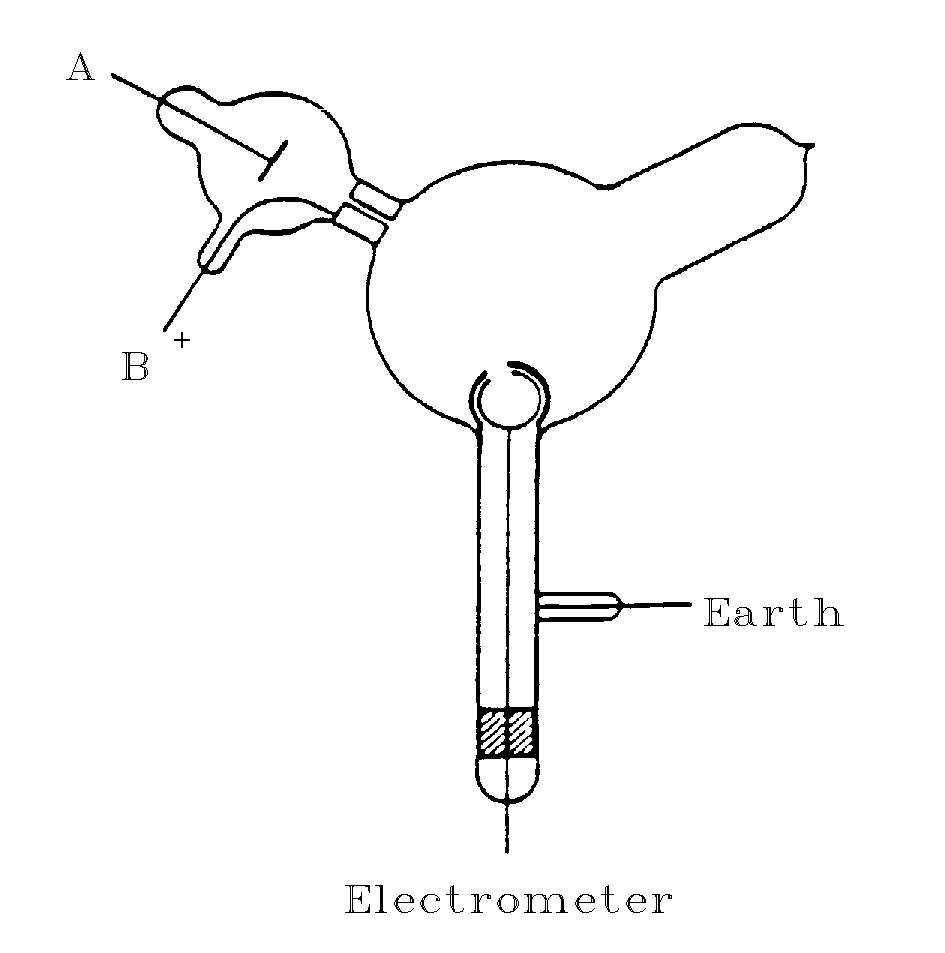
\includegraphics[width=3.17361in,height=3.2in]{images/02_thomson/image007.png}
  \end{center}
  \caption*{Figure 1}
\end{figure}
  

Two coaxial cylinders (Fig.~1) with slits in them are placed in a bulb
connected with the discharge-tube; the cathode rays from the cathode A
pass into the bulb through a slit in a metal plug fitted into the neck
of the tube; this plug is connected with the anode and is put to earth.
The cathode rays thus do not fall upon the cylinders unless they are
deflected by a magnet. The outer cylinder is connected with the earth,
the inner with the electrometer. When the cathode rays (whose path was
traced by the phosphorescence on the glass) did not fall on the slit,
the electrical charge sent to the electrometer when the induction-coil
producing the rays was set in action was small and irregular; when,
however, the rays were bent by a magnet so as to fall on the slit there
was a large charge of negative electricity sent to the electrometer. I
was surprised at the magnitude of the charge; on some occasions enough
negative electricity went through the narrow slit into the inner
cylinder in one second to alter the potential of a capacity of 1.5
microfarads by 20 volts. If the rays were so much bent by the magnet
that they overshot the slits in the cylinder, the charge passing into
the cylinder fell again to a very small fraction of its value when the
aim was true. Thus this experiment shows that however we twist and
deflect the cathode rays by magnetic forces, the negative
electrification is indissolubly connected with the cathode rays.

When the rays are turned by the magnet so as to pass through the slit
into the inner cylinder, the deflexion of the electrometer connected
with this cylinder increases up to a certain value, and then remains
stationary although the rays continue to pour into the cylinder. This is
due to the fact that the gas in the bulb becomes a conductor of
electricity when the cathode rays pass through it, and thus, though the
inner cylinder is perfectly insulated when the rays are not passing, yet
as soon as the rays pass through the bulb the air between the inner
cylinder and the outer one becomes a conductor, and the electricity
escapes from the inner cylinder to the earth. Thus the charge within the
inner cylinder does not go on continually increasing; the cylinder
settles down into a state of equilibrium in which the rate at which it
gains negative electricity from the rays is equal to the rate at which
it loses it by conduction through the air. If the inner cylinder has
initially a positive charge it rapidly loses that charge and acquires a
negative one; while if the initial charge is a negative one, the
cylinder will leak if the initial negative potential is numerically
greater than the equilibrium value.

\subsection*{Deflexion of the Cathode Rays by an Electrostatic Field}

An objection very generally urged against the view that the cathode rays
are negatively electrified particles, is that hitherto no deflexion of
the rays has been observed under a small electrostatic force, and though
the rays are deflected when they pass near electrodes connected with
sources of large differences of potential, such as induction-coils or
electrical machines, the deflexion in this case is regarded by the
supporters of the ætherial theory as primarily due to the discharge
passing between the electrodes, and not primarily to the electrostatic
field. Hertz made the rays travel between two parallel plates of metal
placed inside the discharge-tube, but found that they were not deflected
when the plates were connected with a battery of storage-cells; on
repeating this experiment I at first got the same result, but subsequent
experiments showed that the absence of deflexion is due to the
conductivity conferred on the rarefied gas by the cathode rays. On
measuring this conductivity it was found that it diminished very rapidly
as the exhaustion increased; it seemed then that on trying Hertz's
experiment at very high exhaustions there might be a chance of detecting
the deflexion of the cathode rays by an electrostatic force.

The apparatus used is represented in Figure 2.

\begin{figure}[h]
  \begin{center}
    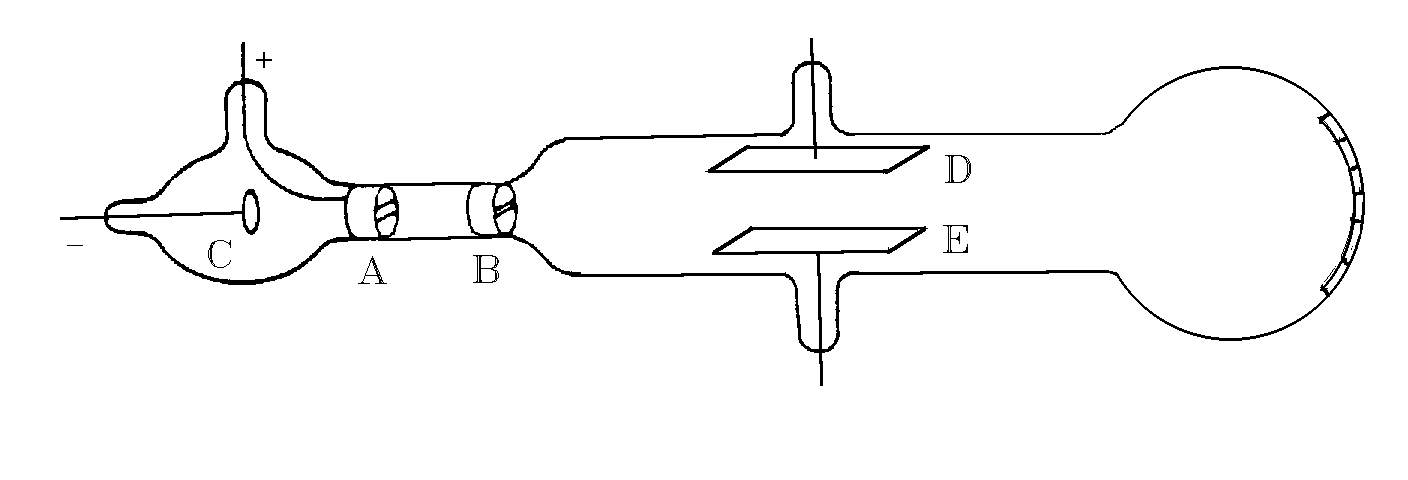
\includegraphics[width=4.69333in,height=1.6in]{images/02_thomson/image009.png}
  \end{center}
  \caption*{Figure 2}
\end{figure}

The rays from the cathode C pass through a slit in the anode A, which is
a metal plug fitting tightly into the tube and connected with the earth;
after passing through a second slit in another earth-connected metal
plug B, they travel between two parallel aluminium plates about 5 cm
long by 2 broad and at a distance of 1.5 cm apart; they then fall on the
end of the tube and produce a narrow well-defined phosphorescent patch.
A scale pasted on the outside of the tube serves to measure the
deflexion of this patch. At high exhaustions the rays were deflected
when the two aluminium plates were connected with the terminals of a
battery of small storage-cells; the rays were depressed when the upper
plate was connected with the negative pole of the battery, the lower
with the positive, and raised when the upper plate was connected with
the positive, the lower with the negative pole. The deflexion was
proportional to the difference of potential between the plates, and I
could detect the deflexion when the potential-difference was as small as
two volts. It was only when the vacuum was a good one that the deflexion
took place, but that the absence of deflexion is due to the conductivity
of the medium is shown by what takes place when the vacuum has just
arrived at the stage at which the deflexion begins. At this stage there
is a deflexion of the rays when the plates are first connected with the
terminals of the battery, but if this connexion is maintained the patch
of phosphorescence gradually creeps back to its undeflected position.
This is just what would happen if the space between the plates were a
conductor, though a very bad one, for then the positive and negative
ions between the plates would slowly diffuse, until the positive plate
became coated with negative ions, the negative plate with positive ones;
thus the electric intensity between the plates would vanish and the
cathode rays be free from electrostatic force.\\
\centerline{* * *}
%
\subsection*{Magnetic Deflexion of the Cathode Rays in Different Gases}
%
\centerline{* * *}

As the cathode rays carry a charge of negative electricity, are
deflected by an electrostatic force as if they were negatively
electrified, and are acted on by a magnetic force in just the way in
which this force would act on a negatively electrified body moving along
the path of these rays, I can see no escape from the conclusion that
they are charges of negative electricity carried by particles of matter.
The next question arises, What are these particles? are they atoms, or
molecules, or matter in a still finer state of subdivision? To throw
some light on this point, I have made a series of measurements of the
ratio of the mass of these particles to the charge carried by it. To
determine this quantity, I have used two independent methods.\footnote{{[}We
  shall consider only the second and more accurate of Thomson's two
  methods.{]}}\\
\centerline{* * *}

I shall describe another method of measuring\footnote{{[}In the
  following, $m$ and $e$ are the mass and charge,
  respectively, and $v$ is the velocity, of a cathode ray particle.
  All of the electric quantities here are expressed in the
  \emph{electromag-netic system of units} (e.m.u.). Thus $e$ is in
  \emph{abcoulombs,} and so on. See Appendix (p.~\pageref{ch:appendix}).{]}} the
quantities $m/e$ and $v$ of an entirely different kind from
the preceding; this method is based upon the deflexion of the cathode
rays in an electrostatic field. If we measure the deflexion experienced
by the rays when traversing a given length under a uniform electric
intensity, and the deflexion of the rays when they traverse a given
distance under a uniform magnetic field, we can find the values of
$m/e$ and $v$ in the following way:---

Let the space passed over by the rays under a uniform electric intensity
\emph{F} be \emph{l},\footnote{{[}Thus \emph{l} is the length of the
  parallel plates D and E in Figure 2.{]}} the time taken for the rays
to traverse this space is $l/v$, the {[}component of the final{]}
velocity in the direction of \emph{F} is therefore
%
\begin{equation*}
\frac{Fe}{m} \cdot \frac{l}{v} \footnote{{[}For this and the next expression see footnote 6, which
  follows.{]}}
\end{equation*}
%
so that $\theta$, the angle through which the rays are deflected when
they leave the electric field and enter a region free from electric
force, is given by the equation
%
\begin{equation*}
\theta = \frac{Fe}{m} \cdot \frac{l}{v^2}. \footnote{{[}The force on the particle is always vertical and of
  magnitude $Fe$. When applied for a time $l/v$ it will impart
  a final vertical velocity $v'$, given by $l/v$ times the
  vertical acceleration, which is $Fe/m$; thus
\begin{equation*}
v' = \frac{Fe}{m} \frac{l}{v}.
\end{equation*}
  Then the vector resultant of horizontal velocity $v$ and vertical
  velocity $v'$ will be directed at an angle $\theta$ such that
\begin{equation*}
\tan{\theta} = \frac{v'}{v} = \frac{Fe}{m} \cdot \frac{l}{v^2}
\end{equation*}
  Moreover for small angles, $\tan{\theta}$ is nearly equal to
  $\theta$ (measured in radians); hence the formula in the text.{]}}
\end{equation*}
%
If, instead of the electric intensity, the rays are acted on by a
magnetic force $H$ at right angles to the rays, and extending
across the distance $l$, then the {[}component of the final{]}
velocity at right angles to the original path of the rays is
%
\begin{equation*}
\frac{Hev}{m} \cdot \frac{l}{v} \footnote{{[}A charge $e$ (e.m.u.), moving with velocity $v$
  at right angles to the direction of a magnetic field $H$, will
  experience a force \emph{f}~=~\emph{Hev}, directed per\-pen\-dic\-u\-larly to
  both $v$ and $H$. (For a discussion see the Note at the end of this chapter.) Now since \emph{a}~=~\emph{f}/\emph{m} and
  \emph{t}~=~\emph{l}/$v$, the charge will attain a {[}component of
  the{]} final velocity $v' = at = \frac{f}{m} \frac{l}{v}$ in the direction per\-pen\-dic\-u\-lar to $v$ and
  $H$. Substitution yields the expression cited.{]}},
\end{equation*}
%
so that $\phi$, the angle through which the rays are deflected when
they leave the magnetic field, is given by the equation
%
\begin{equation*}
\phi = \frac{He}{m} \cdot \frac{l}{v}.\footnote{{[}Obtained by taking the ratio of vertical to horizontal
  components of velocity, just as was done previously for angle
  $\theta$.{]}}
\end{equation*}
%
From these equations we get
\begin{equation*}
v = \frac{\phi}{\theta} \frac{F}{H}
\end{equation*}
and
\begin{equation*}
\frac{m}{e} = \frac{H^{2}\theta l}{F\phi^2}.
\end{equation*}
In the actual experiments $H$ was adjusted so that $\phi =\theta$; in this case the equations become
\begin{align*}
v &= \frac{F}{H} \\ 
\frac{m}{e} &= \frac{H^{2}l}{F\theta}.
\end{align*}

The apparatus used to measure $v$ and $m/e$ by this means is
that represented in Figure 2. The electric field was produced by
connecting the two aluminium plates to the terminals of a battery of
storage-cells. The phosphorescent patch at the end of the tube was
deflected, and the deflexion measured by a scale pasted to the end of
the tube. As it was necessary to darken the room to see the
phosphorescent patch, a needle coated with luminous paint was placed so
that by a screw it could be moved up and down the scale; this needle
could be seen when the room was darkened, and it was moved until it
coincided with the phosphorescent patch. Thus, when light was admitted,
the deflexion of the phosphorescent patch could be measured.

The magnetic field was produced by placing outside the tube two coils
whose diameter was equal to the length of the plates[\ldots].\footnote{{[}We here 
  omit Thomson's description of his method of measuring the magnetic
  field.{]}}\\
\centerline{* * *}

A series of experiments was made to see if the electrostatic deflexion
was proportional to the electric intensity between the plates; this was
found to be the case. In the following experiments the current through
the coils was adjusted so that the electrostatic deflexion was the same
as the magnetic:---

\begin{center}
\begin{tabular}{l*{6}{c}}
\multicolumn{6}{c}{TABLE 1}\\
\hline
\emph{Gas.} & $\theta.$ & $H.$ & $F.$ & $l.$ & $m/e.$ & $v.$\\
Air           & 8/100   & 5.5 & $1.5\!\times\!{10^{10}}$ & 5 & $1.3\!\times\!{10^{-7}}$ & $2.8\!\times\!{10^9}$\\
Air           & 9.5/100 & 5.4 & $1.5\!\times\!{10^{10}}$ & 5 & $1.1\!\times\!{10^{-7}}$ & $2.8\!\times\!{10^9}$\\
Air           & 13/110  & 6.6 & $1.5\!\times\!{10^{10}}$ & 5 & $1.2\!\times\!{10^{-7}}$ & $2.3\!\times\!{10^9}$\\
Hydrogen      & 9/110   & 6.3 & $1.5\!\times\!{10^{10}}$ & 5 & $1.5\!\times\!{10^{-7}}$ & $2.5\!\times\!{10^9}$\\
Carbonic acid & 11/110  & 6.9 & $1.5\!\times\!{10^{10}}$ & 5 & $1.5\!\times\!{10^{-7}}$ & $2.2\!\times\!{10^9}$\\
Air           & 6/110   & 5   & $1.8\!\times\!{10^{10}}$ & 5 & $1.3\!\times\!{10^{-7}}$ & $3.6\!\times\!{10^9}$\\
Air           & 7/110   & 3.6 & $1\!\times\!{10^{10}}$   & 5 & $1.1\!\times\!{10^{-7}}$ & $2.8\!\times\!{10^9}$\\
\hline
\end{tabular}
\end{center}

The cathode in the first five experiments was aluminium, in the last two
experiments it was made of platinum; in the last experiment Sir William
Crookes's method of getting rid of the mercury vapour by inserting tubes
of pounded sulphur, sulphur iodide, and copper filings between the bulb
and the pump was adopted. In the calculation of $m/e$ and $v$
no allowance has been made for the magnetic force due to the coil in the
region outside the plates; in this region the magnetic force will be in
the opposite direction to that between the plates, and will tend to bend
the cathode rays in the opposite direction: thus the effective value of
H will be smaller than the value used in the equations, so that the
values of $m/e$ are larger and those of $v$ less than they
would be if this correction were applied\ldots.\footnote{{[}The value of
  \emph{m}/$e$ accepted today is $0.5685\!\times\!10^{-7}$ g/abC, less than
  half the average of the values given in Thomson's table above. Thomson
  acknowledges that he has neglected the magnetic field \emph{outside}
  the parallel plates. Although he does not appear to regard that as a
  serious omission, it may in fact account for much of the discrepancy
  between his results and subsequent determinations.{]}}

From these determinations we see that the value of \emph{m/e} is
independent of the nature of the gas, and that its value $10^{-7}$ is very
small compared with the value $10^{-4}$, which is the smallest value of this
quantity previously known, and which is the value for the hydrogen ion
in electrolysis.\footnote{{[}Thomson here alludes to the results of
  electrolysis experiments such as our electroplating exercise: that one
  gram-equivalent weight of any element is associated with a charge of
  96,500 coulombs (9,650 abcoulombs). Then since 1 gram is the
  gram-equivalent weight of hydrogen, the quotient \emph{m/e} for
  hydrogen will be 1/9,650 g/abC, or approximately $10^{‑4}$, as Thomson
  cites.{]}}

Thus for the carriers of the electricity in the cathode rays $m/e$
is very small compared with its value in electrolysis. The smallness of
$m/e$ may be due to the smallness of $m$ or the largeness of
$e$, or to a combination of these two. That the carriers of the
charges in the cathode rays are small compared with ordinary molecules
is shown, I think, by Lenard's results as to the rate at which the
brightness of the phosphorescence produced by these rays diminishes with
the length of path traveled by the ray. If we regard this
phosphorescence as due to the impact of the charged particles, the
distance through which the rays must travel before the phosphorescence
fades to a given fraction (say, $1/e$, where $e = 2.71$)
of its original intensity, will be some moderate multiple of the mean
free path.\footnote{{[}Here, $e$ is the
  base of the natural log system, approximately 2.71, and should not be
  confused with $e$, the charge carried by a cathode ray
  ``corpuscle.'' The \emph{mean free path} of a molecule in a gas is the
  average distance it can travel before colliding with another molecule.
  For air at atmospheric pressure this distance is of the order of one
  millionth of 1 cm.{]}} Now Lenard found that this distance depends
solely upon the density of the medium, and not upon its chemical nature
or physical state. In air at atmospheric pressure the distance was about
half a centimetre, and this must be comparable with the mean free path
of the carriers through air at atmospheric pressure. But the mean free
path of the molecules of air is a quantity of quite a different order.
The carrier, then, must be small compared with ordinary molecules.\\
\centerline{* * *}

The explanation which seems to me to account in the most simple and
straight\-for\-ward manner for the facts is founded on a view of the
constitution of the chemical elements which has been favourably
entertained by many chemists: this view is that the atoms of the
different chemical elements are different aggregations of atoms of the
same kind. In the form in which this hypothesis was enunciated by
Prout,\footnote{{[}William Prout (1785-1850), English chemist and
  physician, pointed out in an anonymous article in the \emph{Annals of
  Philosophy} in 1815 that the atomic weights of a number of elements
  are multiples of that of hydrogen. In a second article in the
  following year he suggested that hydrogen was the ``prime matter'' of
  the ancients.{]}} the atoms of the different elements were hydrogen
atoms; in this precise form the hypothesis is not tenable, but if we
substitute for hydrogen some unknown primordial substance X, there is
nothing known which is inconsistent with this hypothesis[\ldots].

If, in the very intense electric field in the neighborhood of the
cathode, the molecules of the gas are dissociated and are split up, not
into the ordinary chemical atoms, but into these primordial atoms, which
we shall for brevity call corpuscles; and if these corpuscles are
charged with electricity and projected from the cathode by the electric
field, they would behave exactly like the cathode rays. They would
evidently give a value of \emph{m/e} which is independent of the nature
of the gas and its pressure, for the carriers are the same whatever the
gas may be[\ldots].

Thus we have in the cathode rays matter in a new state, a state in which
the sub\-di\-vi\-sion of matter is carried very much further than in the
ordinary gaseous state: a state in which all matter---that is, matter
derived from different sources such as hydrogen, oxygen, \&c.---is of
one and the same kind; this matter being the substance from which all
the chemical elements are built up.\\
\centerline{* * *}
%
\section*{Experiment: The Ratio of Charge to Mass in Cathode Rays}

The cathode-ray tube de\-scribed here operates on the same principles as
does that de\-scribed by Thomson. However, the experiment is made somewhat
more elegant by causing the cathode-ray particles to orbit in a circular
path under the action of the magnetic field alone. This happens because
in a magnetic field $H$ the force on a charge $e$ moving with
velocity $v$ is always per\-pen\-dic\-u\-lar to both $H$ and $v$.
Thus if $v$ is initially per\-pen\-dic\-u\-lar to $H$ and if $H$
is uniform, the forces on $e$ will always deflect it in a single
plane per\-pen\-dic\-u\-lar to $H$, as diagrammed in the figure
below.\footnote{If in the figure the indicated direction for the force
  \emph{f} seems to be reversed, recall that the charge on the
  hypothetical cathode-ray particle is \emph{negative}.} Moreover, since
force \emph{f} is also normal to $v$, the charge $e$ will
never be accelerated in the direction of its motion, and $v$ will
therefore remain constant in magnitude and vary only in direction. But
these are exactly the conditions for circular motion with constant
speed; in such an orbit the force is always normal to the velocity and
is directed to a virtual center, O.

\begin{figure}[h]
  \begin{center}
    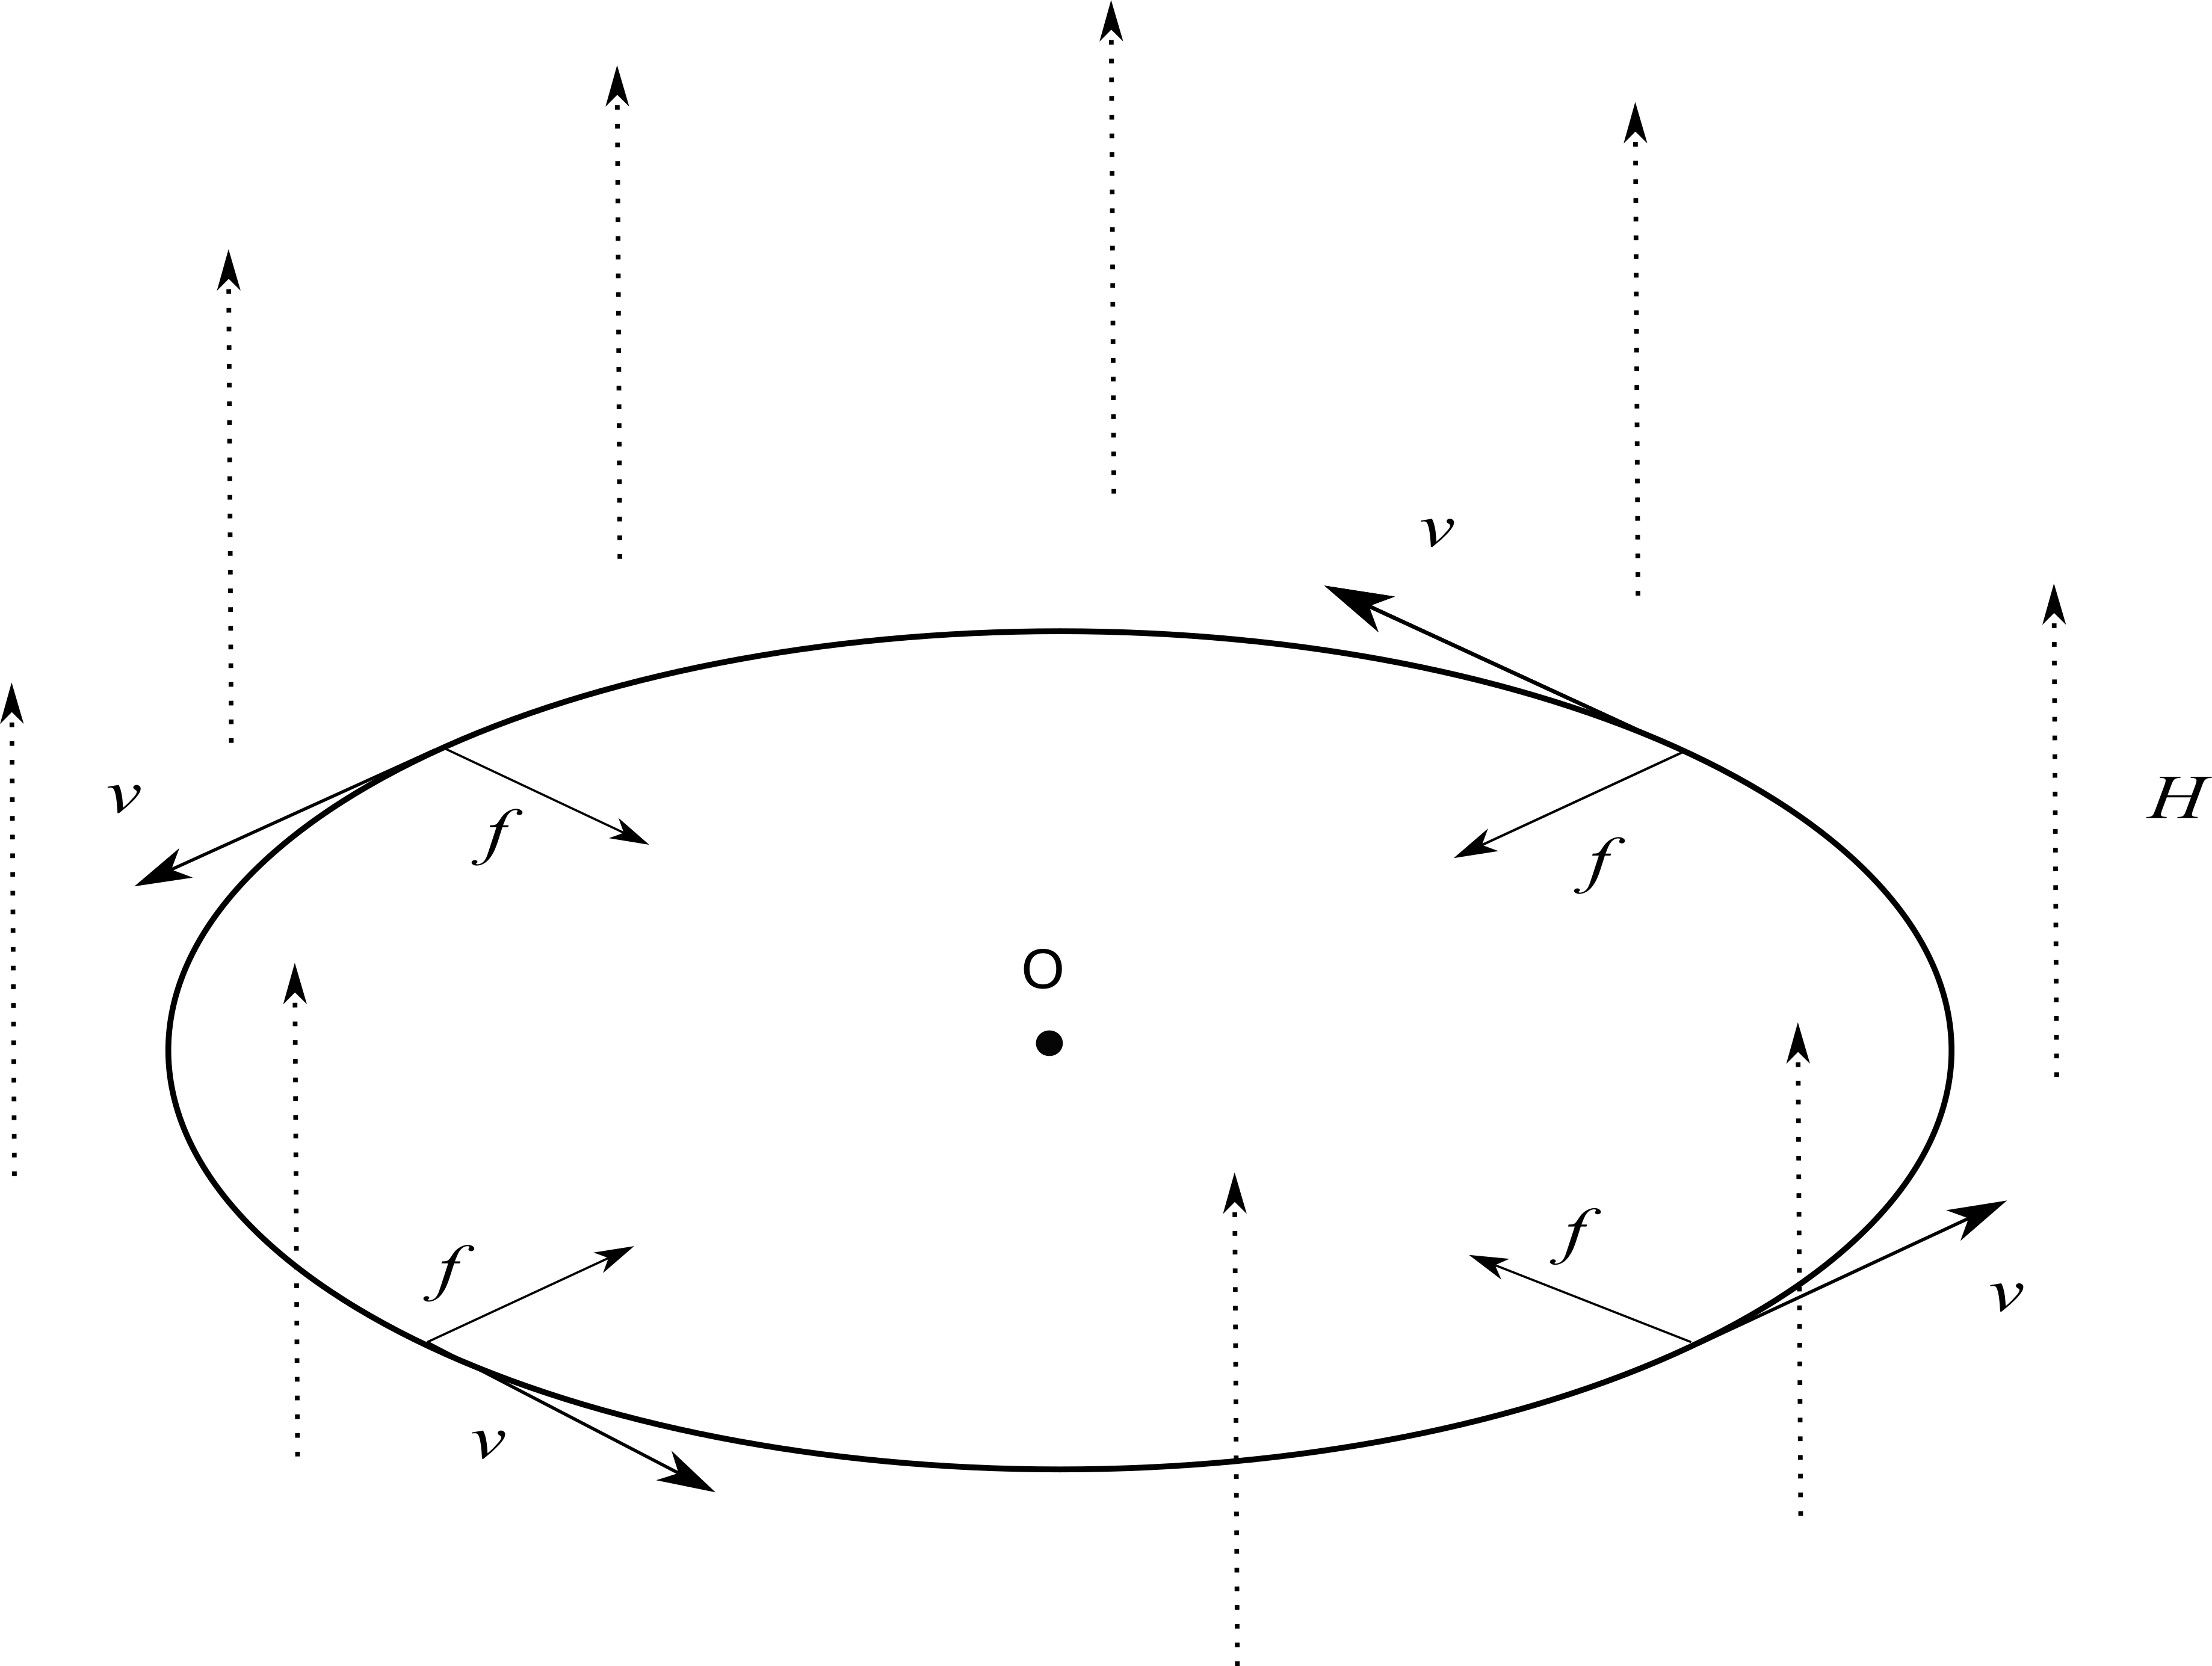
\includegraphics[width=0.75\textwidth]{images/02_thomson/image099.png}
  \end{center}
\end{figure}

Now the acceleration $a$ towards the center of circular motion is
$a = v^2/r$,\footnote{Cf. Newton, \emph{Principia},
  Prop.\ IV, Corollary 1.} so that the central force will be given by
%
\begin{equation}
f = ma = mv^2/r.\label{eq:f=ma_thomson}
\end{equation}
%
In the present case the force $f$ is supplied by the magnetic field
and is therefore\footnote{See the Note at the end of this chapter (p.~\pageref{n:thomson}).}
\begin{equation}
f = Hev\label{eq:f=Hev_thomson}
\end{equation}
(compare Thomson's equation for magnetic deflection). Combining
equations \eqref{eq:f=ma_thomson} and \eqref{eq:f=Hev_thomson}, we find
\begin{equation}
\frac{e}{m} = \frac{v}{rH};\label{eq:em=vrH_thomson}
\end{equation}
the ratio $e/m$ will thus be known if $r$, $H$, and
$v$ are known. We use a tube in which several radii $r$
are marked on a phosphor-coated scale running the length of the tube; 
the magnetic field $H$ is adjusted
until the ray orbit intersects the scale at a predetermined marking indicating 
the diameter (e.g., 10 cm), and thus $r$ is
known. It remains only to determine $H$ and $v$.

\begin{figure}[h]
  \begin{center}
    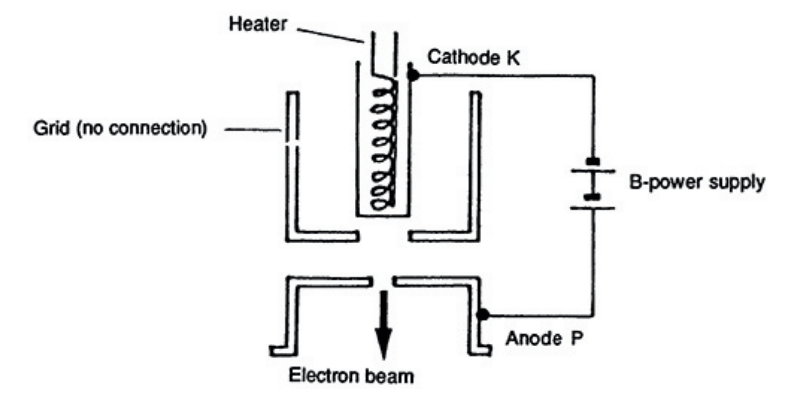
\includegraphics[width=2.63in,height=1.36667in]{images/02_thomson/gun.png}
  \end{center}
\end{figure}


The tube with its connections is diagrammed in the sketches. It contains
an anode and a heated cathode. A power supply maintains the anode at a positive
potential with respect to the cathode, so that negative particles emitted
by it are accelerated towards the anode and pass through the slit with
considerable velocity. Current is run through a pair of coils that surrounds the tube, arranged so that 
their magnetic fields combine to form a nearly uniform field in the region of the tube. The beam of 
particles is indicated by the glow of vapor in the tube; coil current is adjusted until 
the orbit of the particles lines up with one of the marks for measurement.

\begin{figure}[h]
  \begin{center}
    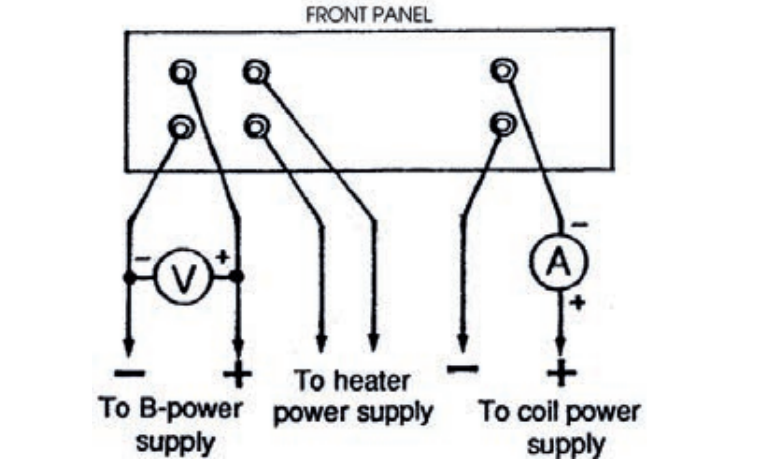
\includegraphics[width=2.59in,height=1.53667in]{images/02_thomson/power-supply.png}
  \end{center}
\end{figure}



Energy considerations determine the velocity $v$. Since particles
emitted from the cathode are accelerated to the anode, they gain kinetic
energy equal to the work done by the electric field on them. This work
equals the product of the potential difference and the charge on the
particle,\footnote{See Appendix (p.~\pageref{ch:appendix}).} so that in electromagnetic
units ($V$ in abvolts and $e$ in abcoulombs), we have
%
\begin{equation}
Ve = \frac{1}{2}mv^2 \quad\text{or}\quad v = \sqrt{\frac{2Ve}{m}}.\label{eq:Ve/v_thomson}
\end{equation}
%
If $V$ represents the measurement in \emph{volts} as per our
meters, a conversion factor must be introduced ($1$ volt = $10^8$ abvolts),
and the equation becomes
\begin{equation}\tag{5}
v = \sqrt{\frac{2V_{volt}e\cdot{10^8}}{m}}
\end{equation}
Substitution of this value in equation (3) yields for $e/m$:
\begin{equation}\tag{6}
\frac{e}{m} = \frac{2V_{volt}}{r^2H^2}\cdot 10^8 \:\text{abC/g.}
\end{equation}

\begin{wrapfigure}[11]{r}{2.75in}
  \begin{center}
    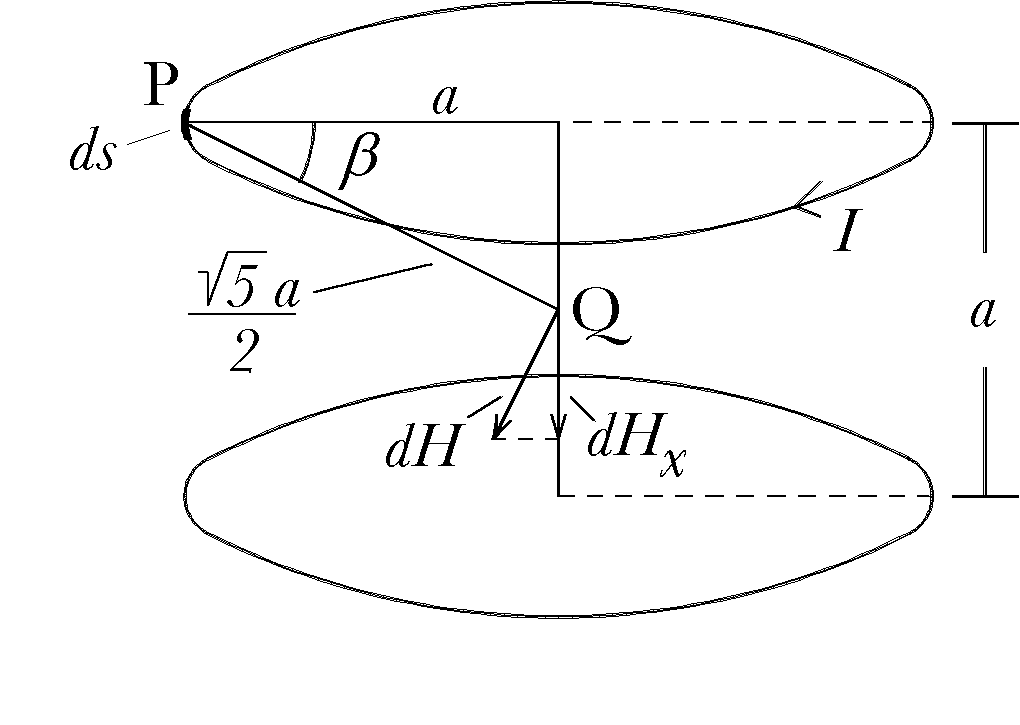
\includegraphics[width=2.72153in,height=1.93056in]{images/02_thomson/image039.png}
  \end{center}
\end{wrapfigure}

%\includegraphics[width=2.72153in,height=1.93056in]{media/image23.png}

Finally, the magnetic field $H$ must be found. The pair of coils we
use, known as Helmholtz coils, is so designed that the distance between
them is equal to the coil radius $a$. (This makes the magnetic field
between the coils relatively uniform.) The tube is placed at Q,
which is at a distance $a/2$ from the center of each coil. The
contribution $dH$ that a current element $I\,ds$ at P makes to
the field at Q will be
\begin{equation*}
dH = \frac{I\,ds}{PQ^2} = \frac{I\,ds}{(5/4)a^2} = \frac{4}{5}\frac{I\,ds}{a^2}
\end{equation*}
(using the Pythagorean Theorem to give us PQ$^2$). As
successive current elements are considered, components of \emph{dH}
per\-pen\-dic\-u\-lar to the axis cancel one another, so that only axial
components $dH_x$ are effective. But
\begin{equation*}
\cos{\beta} = a/PQ = 2/\sqrt{5},
\end{equation*}
whence
\begin{equation}\tag{7}
dH_x = dH \cos{\beta} = \frac{2}{\sqrt{5}}dH = \frac{8}{5\sqrt{5}}\frac{I\,ds}{a^2}.
\end{equation}
Integrating, we obtain
\begin{equation*}
H = \int_{0}^{2\pi{a}} \frac{8}{5\sqrt{5}}\frac{I}{a^2}\,ds = \frac{8}{5\sqrt{5}}\frac{2\pi aI}{a^2} = \frac{16\pi I}{5\sqrt{5}a}.
\end{equation*}
For \emph{two} coils of \emph{N} turns each, therefore,
\begin{equation*}
H = \frac{32\pi IN}{5\sqrt{5}a}.
\end{equation*}
If the current $I$ is stated in \emph{amperes} as per our meter
readings, the above equation becomes
\begin{equation}\tag{8}
H = \frac{3.2\pi NI_{amp}}{5\sqrt{5}a}.
\end{equation}
For our coils, $N$ = 130.

Thus we use equation (8) to determine the magnetic field $H$; then
we substitute this value into equation (6) to determine the
charge-to-mass ratio $e/m$.

\subsubsection*{Operation}

When the apparatus is wired, orient the coils so their axis is aligned
with magnetic north in the room (use a compass for
this purpose). Slowly raise $V$, the anode voltage, to some value between 200 and 300 volts. 
Record this voltage, and vary the coil current $I$ until the beam falls on one
of the markers. Half of this diameter will be your radius $r$ for equation (6). 
With known $I$ we calculate $H$ using equation
(7); then with known $H$ and $V$ and $r$ we calculate
$e/m$ using equation (5). It makes sense to determine $e/m$
several times using different radii and different voltages. Although by
our theory the values thus obtained ought to agree, in practice they may
differ. If so, look for any suggestive regularities in the differences;
for example, are measurements taken at higher voltages uniformly greater
or less than those taken at lower voltages? What might cause such an
effect?


\section*{Note: On Magnetic Fields and Moving Charged Bodies}\label{n:thomson}

A current-carrying wire, because of the magnetic field which it generates,
will exert a force on any magnet placed near it. By Newton's Third Law,
the magnet will necessarily exert \emph{an equal and opposite force back
on the wire}. Thus, magnetic fields exert force on current-carrying
wires. If a long straight wire carrying a current of 1 abampere is
placed in a perfectly uniform magnetic field of unit strength with the
field lines perpendicular to the wire, then it will experience \emph{a
force of one dyne for every centimeter of its length}. The force will be
perpendicular to both the wire and the field lines.

An analogous situation holds for \emph{moving charged bodies} in a
magnetic field. A body carrying 1 abcoulomb and moving at 1 centimeter
per second through a magnetic field of unit strength will experience a
force of \emph{1 dyne} perpendicular to both the field lines and the
direction of motion. We cannot argue rigorously for this here, but note
that in one second this charged body makes one abcoulomb ``flow'' a
distance of one centimeter---just as does a 1-cm-long wire carrying 1
abamp, which also would experience a force of one dyne. At any rate, in
general
\begin{equation*}
f = Hev ,
\end{equation*}
where $f$ is the force, $H$ is the magnetic field strength,
$e$ is the charge \emph{in abamperes} and $v$ is the velocity
in cm./sec.

For both the current-carrying wire and the moving charged particle, the
direction of the force is more or less conveniently given by the ``left
hand rule,'' also known as the ``\emph{fBI''} rule. Arrange the thumb,
forefinger and middle fingers on your left (your \emph{left}) hand so
that they are mutually perpendicular, like 3-dimensional coordinate
axes. Then your thumb will give the direction of \emph{f} the force if
your forefinger points in the direction of \emph{B} the magnetic field
and your middle finger in the direction of \emph{I} the current.
(Remember that for a cathode-ray current, \emph{I} is in the opposite
direction of the motion of the electrons, since they are negatively
charged.)

\chapter{The Electron}

\chapterprecis{R.\ A.\ Millikan}

\makeoddhead{myheadings}{\emph{Millikan}}{}{\thepage}
\makeevenhead{myheadings}{\thepage}{}{\emph{The Electron}}

\section*{Remarks}

\indent
We turn now to the examination of ``charge'' itself, in particular to
the question whether charge is discrete or continuous in its ultimate
composition. That question was ef\-fec\-tive\-ly answered with R.\ A.\ 
Millikan's discovery of a fundamental unit of charge---the so-called
``electron.''

The instrument Millikan employed for that delicate task of measurement
is a tiny droplet of oil bearing a minute electrical charge, alternately
hoisted up by an applied electric field, then allowed to fall back down
under its own weight with the field turned off. From observations of the
motion of such drops Millikan was able, first, to show that a
fundamental unit of charge \emph{exists}; second, to determine the
magnitude of that unit.

In the selection that follows, Millikan takes as granted the equations
governing the motion of the oil drop. Therefore the first phase in our
reasoning must be to work out in a general way the forces that act on
the drop and to derive the equation of its motion under those forces. It
will be assumed at this point that the size and mass of the drop are
known; actually their determination constitutes an important second
phase of the analysis.

\begin{figure}[h]
  \begin{center}
    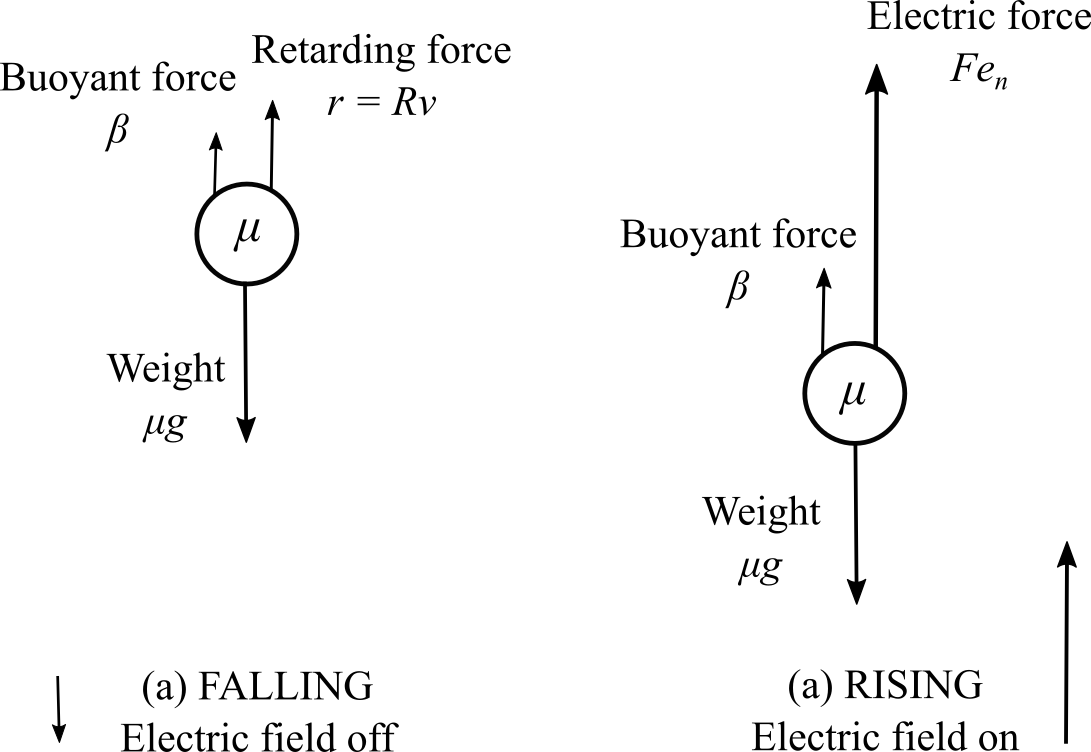
\includegraphics[width=3.63667in]{images/03_millikan/drops.png}
  \end{center}
\end{figure}

The forces which act on a falling drop in the absence of an electric
field are sketched on the left side of the diagram, marked (a). The mass 
of the drop is $\mu$ and the weight is therefore $\mu g$. The drop falls 
through the air, which we shall regard as a very thin homogeneous fluid that 
both buoys up a body and resists motion through itself. We also assume, with 
Millikan, that this resisting force is \emph{directly proportional to the 
velocity} of the moving drop. This proportionality characterizes the special 
type of friction called a ``viscous'' force, exerted by a ``viscous'' fluid 
on any body moving through it. The measure of a fluid's capacity for
applying such a force is called its ``viscosity.'' Millikan had good
reason to believe that air exhibited this viscosity quite strictly.

With some constant of proportionality, $R$, then, the viscous force
$r$ resisting the droplet's fall will be

\begin{equation*}\tag{3.1}
r = Rv
\end{equation*}
%
as shown in Fig. (a).

At the same time, the drop is buoyed up by a force equal to the weight
of air which it displaces.\footnote{Archimedes, \emph{On Floating
  Bodies}, I, Prop.\ 7.} Thus a droplet of volume $V$ will have mass
$\mu = V\sigma$, but it will displace a mass $V\rho$ of air,
where $\sigma$ is the density of the oil and $\rho$ is the density of
the air. Hence the three forces acting on the falling drop are:

\begin{align*}
\text{Weight}\quad W & = V\sigma g\\
\text{Buoyancy}\quad \beta & = V\rho g\\
\text{Retarding force}\quad r &= Rv\\
\end{align*}
%
for a total downward force $f$ of
%
\begin{align*}
f &= V\sigma g-V\rho g-Rv\\
 &= V(\sigma-\rho)g-Rv\\
\end{align*}

On analogy with $V\sigma$, the actual mass of the oil drop, Millikan
will call $V(\sigma-\rho)$ in the expression above the
``effective'' grav\-i\-ta\-tion\-al mass, $m$---as though the reduced
downward tendency of the drop in the buoyant medium were due to a
reduced grav\-i\-ta\-tion\-al mass $m = V(\sigma-\rho)$
rather than, as is actually the case, to the presence of an upward
buoyant force $\beta = V\rho g$. The expression for the net downward
force can then be written
\begin{equation*}\tag{3.2}
f = mg - Rv
\end{equation*}
where $m = V(\sigma-\rho)$. There will be a downward
acceleration---that is, a continuing increase in velocity $v$---so
long as the resistance $Rv$ of the medium is less than the
effective weight $mg$.

However, as the velocity of the drop increases, so will the resistance;
as $Rv$ increases it will approach $mg$ and the net force
$f$ will approach zero, as is clear from equation (3.2) above. The
acceleration will become very small, and the droplet will continuously 
approach the \emph{constant} velocity $v_1$,\footnote{In practice, the drop
almost immediatley accelerates to a velocity immeasurably close to its terminal 
velocity.} characterized as the velocity at which
\begin{equation*}
Rv = mg.
\end{equation*}
%
This gives
\begin{equation*}\tag{3.3}
v_1 = \frac{mg}{R}.
\end{equation*}

Suppose now that the droplet bears electric charge $e_n$. In the
absence of an electric field, that charge will not affect the drop's
motion. But when a field $F$ tending to raise the drop is applied,
an upward force $Fe_n$ will act on the drop; and if it is strong
enough to overbalance the effective weight of the drop, the drop will
stop falling and begin to rise. Then while the drop is rising both the
effective weight and the viscous force will be \emph{downwards}, and
there will act on the drop (see Fig. (b)) a net \emph{upward} force
equal to
\begin{equation*}
Fe_n - mg - Rv.
\end{equation*}
Then by an argument similar to that for the drop when falling, the
rising drop will shortly attain a constant upward velocity $v_2$,
where
\begin{equation*}\tag{3.4}
v_2=\frac{Fe_n - mg}{R}
\end{equation*}
It is a striking characteristic of motion in a viscous medium that a
body under the action of a constant force attains a \emph{constant
velocity proportional to that force}.

Equations (3.3) and (3.4) constitute all the theory that Millikan
requires to establish from his observations that the electron
\emph{exists}; although calculation of its \emph{quantity} involves, as
we shall see, considerably more reasoning. Actually Millikan uses the
\emph{quotient} of equation (3.3) by equation (3.4), which is
\begin{center}
\begin{align*}\tag{1}
\frac{v_1}{v_2} = \frac{mg}{Fe_n - mg} \quad\text{or}\quad & e_n = \frac{mg}{Fv_1}(v_1 + v_2)
\end{align*}
\end{center}
It will be called equation (9) in the selection that follows.

A final remark: unlike Thomson (who had to deal with both electric and
magnetic qualities in his calculations), Millikan, who deals with the
electron only in its e\-lec\-tro\-stat\-ic relations, accordingly uses the
\emph{e\-lec\-tro\-stat\-ic system of units} (e.s.u.) in what we are about to
read. Thus he will eventually state his fundamental unit of charge in
\emph{stat\-cou\-lombs.} In order to relate Millikan's and Thomson's
results, recall that the electromagnetic and the e\-lec\-tro\-stat\-ic systems
of units are related by the constant \emph{c} (the speed of light in 
centimeters per second), so that one abcoulomb
equals $3.00 \times 10^{10}$ stat\-cou\-lombs. (See Appendix below
for a fuller discussion of the relation between the ``e\-lec\-tro\-stat\-ic''
and ``electromagnetic'' system of units.)

\section*{The Electron\\ {\large R.\ A.\ Millikan}}

\subsection*{General Proof of the Atomic Nature of Electricity\footnote{[Chapter IV of \emph{The Electron}, University of
  Chicago Press (1924). Although we are reading his 1924 account,
  Millikan developed the methods here described from 1909 to 1913.]}}


Although the ``balanced droplet method'' just described\footnote{{[}Millikan
  here refers to an earlier technique, omitted here.{]}} had eliminated
the chief sour\-ces of uncertainty which inhered in preceding work on
\emph{e} and had made it possible to assert with much confidence that
the unit charge was a real physical entity and not merely a
``statistical mean,'' it was yet very far from an exact method of
studying the properties of gaseous ions. The sour\-ces of error or
uncertainty which still inhered in it arose from (1) the lack of
stagnancy in the air through which the drop moved; (2) the lack of
perfect uniformity of the electrical field used; (3) the gradual
evaporation of the drops, rendering it impossible to hold a given drop
under observation for more than a minute or to time a drop as it fell
under gravity alone through a period of more than five or six seconds;
and (4) the assumption of the validity of Stokes's Law.

The method which was devised to replace it was not only entirely free
from all of these limitations, but it constituted an entirely new way of
studying ionization and one which at once yielded important results in a
considerable number of directions. This chapter deals with some of these
by-products of the determination of \emph{e} which are of even more
fundamental interest and importance than the mere discovery of the exact
size of the electron.

\subsection*{I. Isolation of Individual Ions and Measurement of Their Relative Charges}

In order to compare the charges on different ions, the procedure adopted
was to blow with an ordinary commercial atomizer an oil spray into the
chamber C (Fig. 3). The air with which this spray was blown was first
rendered dust-free by passage through a tube containing glass wool. The
minute droplets of oil constituting the spray, most of them having a
radius of the order of a one-thousandth of a millimeter, slowly fell in
the chamber C, and occasionally one of them would find its way through
the minute pinhole \emph{p} in the middle of the circular brass plate M,
\begin{figure}[h]
  \begin{center}
    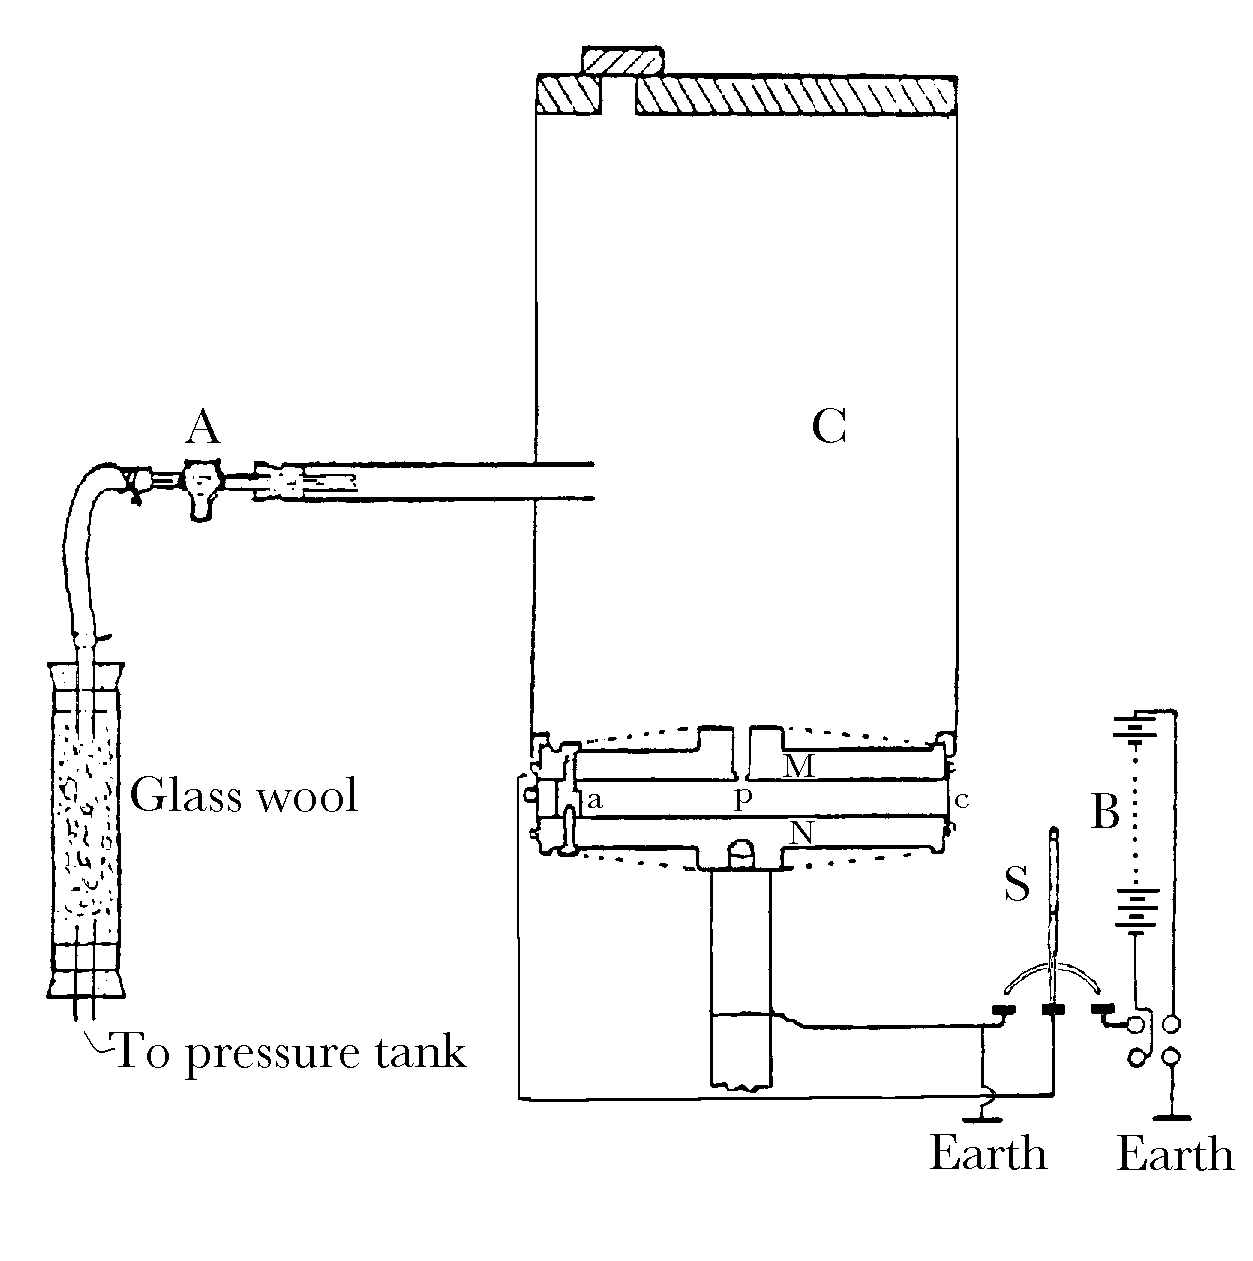
\includegraphics[width=0.6\textwidth]{images/03_millikan/image013.png}
  \end{center}
  \caption*{Figure 3}
\end{figure}
22 cm in diameter, which formed one of the plates of the air condenser.
The other plate, N, was held 16 mm. beneath it by three ebonite posts
\emph{a}. By means of the switch S these plates could be charged, the
one positively and the other negatively, by making them the terminals of
a 10,000-volt storage battery B, while throwing the switch the other way
(to the left) short-circuited them and reduced the field between them to
zero. The oil droplets which entered at \emph{p} were illuminated by a
powerful beam of light which passed through diametrically opposite
windows in the encircling ebonite strip \emph{c}. As viewed through a
third window in \emph{c} on the side toward the reader, it appeared as a
bright star on a black background. These droplets which entered \emph{p}
were found in general to have been strongly charged by the frictional
process involved in blowing the spray, so that when the field was thrown
on in the proper direction they would be pulled up toward M. Just before
the drop under observation could strike M the plates would be
short-circuited and the drop allowed to fall under gravity until it was
close to N, when the direction of motion would be again reversed by
throwing on the field. In this way the drop would be kept traveling back
and forth between the plates. The first time the experiment was tried an
ion\footnote{{[}``Ion'' was Faraday's term for the particles of matter
  which seemed, in electrolysis, to migrate from one region of the
  solution to another. Although Faraday himself distrusted the atomic
  view, researchers of a later generation collected much evidence that
  ``ions'' were actually \emph{electrically-charged atoms} (or groups of
  atoms), which were not only found in electrolytes but could also be
  produced in gases by various causes including x-rays and the presence
  of radioactive substances. In an earlier chapter of \emph{The
  Electron}, Millikan wrote: ``In a word, then, the act of ionization in
  gases appears to consist in the detachment from a neutral atom of one
  or more negatively charged particles, called by Thomson
  \emph{corpuscles}. The residuum of the atom is of course positively
  charged\ldots. The detached corpuscle must soon attach itself, in a
  gas at ordinary pressure, to a neutral atom.'' Thus some of the air
  molecules in Millikan's chamber carry either a positive or a negative
  charge, and it is these charged molecules---ions---that periodically
  collide with the oil drop and yield to it whatever charges they
  bear.{]}} was caught within
%
\begin{table}[htp]
\centering
%\begin{center}
\begin{tabular}{S c c c c S}
\multicolumn{6}{c}{\hspace{2em} TABLE IV}\\
$t_g$ & & & & $t_F$\\[2pt]
13.6 & & & & 12.5\\
13.8 & & & & 12.4&\\
13.4 & & & & 21.8&\\
13.4 & & & & 34.8&\\
13.6 & & & & 84.5&\\
13.6 & & & & 85.5&\\
13.7 & & & & 34.6&\\
13.5 & & & & 34.8&\\
13.5 & & & & 16.0&\\
13.8 & & & & 34.8&\\
13.7 & & & & 34.6&\\
13.8 & & & & 21.9&\\
13.6&\\
13.5&\\
13.4&\\
13.8&\\
13.4&\\[-8pt]
\underline{\phantom{013.1}}\\
\text{Mean} 13.595&\\
\end{tabular}
\end{table}
%\end{center}
%
a few minutes, and the fact of its capture was signaled to the observer
by the change in the speed with which {[}the oil drop{]} moved up when
the field was on. The significance of the experiment can best be
appreciated by examination of the complete record of one of the early
experiments when the timing was done merely with a stop watch.

The column headed $t_g$ gives the successive times which the droplet
required to fall [under the force of gravity, $g$] between two fixed cross-hairs in the observing
telescope whose distance apart corresponded in this case to an actual
distance of fall of .5222 cm. It will be seen that these numbers are all
the same within the limits of error of a stop-watch measurement. The
column marked $t_F$ gives the successive times which the droplet
required to rise under the influence of the electrical field [$F$] produced by
applying in this case 5,051 volts of potential difference to the plates
M and N. It will be seen that after the second trip up, the time changed
from 12.4 to 21.8, indicating, since in this case the drop was positive,
that a negative ion had been caught from the air. The next time recorded
under $t_F$, namely, 34.8, indicates that another negative ion had
been caught. The next time, 84.5, indicates the capture of still another
negative ion. This charge was held for two trips, when the speed changed
back again to 34.6, showing that a positive ion had now been caught
which carried precisely the same charge as the negative ion which before
caused the inverse change in time, i.e., that from 34.8 to 84.5.

In order to obtain some of the most important consequences of this and
other similar experiments we need make no assumption further than this,
that the velocity with which the drop moves is proportional to the force
acting upon it and is independent of the electrical charge which it
carries. Fortunately this assumption can be put to very delicate
experimental test, as will presently be shown, but introducing it for
the time being as a mere assumption, as Townsend, Thomson, and Wilson
had done before, we get
%
\begin{center}
\begin{align*}\tag{9}
\frac{v_1}{v_2} = \frac{mg}{Fe_n-mg} \quad\text{or}\quad & e_n = \frac{mg}{Fv_1}(v_1+v_2)
\end{align*}
\end{center}
%
The negative sign is used in the denominator because $v_2$ will for
convenience be taken as positive when the drop is going up in the
direction of \emph{F}, while $v_1$ will be taken as positive when it
is going down in the direction of \emph{g}. $e_n$ denotes the charge
on the drop, and must not be confused with the charge on an ion. If now
by the capture of an ion the drop changes its charge from $e_n$ to
$e_{n'}$, then the value of the captured charge $e_i$ is
\begin{equation*}\tag{10}
e_i = e_{n'}-e_n=\frac{mg}{Fv_1}(v_{2}'-v_2)
\end{equation*}
and since $mg/Fv_1$ is a constant for this drop, any charge which it
may capture will always be proportional to ($v_{2}'-v_2$),
that is, to the change produced in the velocity in the field \emph{F} by
the captured ion. The successive values of $v_2$ and of ($v_{2}'-v_2$) 
are shown in Table V.

\begin{table}[htp]
\centering
\begin{minipage}{\textwidth}
\centering
\begin{tabular}{ c c }
  \multicolumn{2}{c}{TABLE V\footnote{[The bracketed numbers are our corrections of typos
  in Millikan's original table.]}}\\
  $v_2$ & $ (v'_2 - v_2)$\\
  &\\
  $\frac{.5222}{12.45} = .04196$ & \multirow{3}{*}{$\biggr\} .01806 \div 2 = .00903$}\\
  &\\
  $\frac{.5222}{{[}21.85{]}} = .02390$ & \multirow{3}{*}{$\biggr\} .00885 \div 1 = .00885$}\\
  &\\
  $\frac{.5222}{34.7} = .01505$ &\multirow{3}{*}{$\biggr\} .00891 \div 1 = .00891$}\\
  &\\
  $\frac{.5222}{85.0} = .006144$ &\multirow{3}{*}{$\biggr\} .00891 \div 1 = .00891$}\\
  &\\
  $\frac{.5222}{34.7} = .01505$ &\multirow{3}{*}{$\biggr\} .01759 \div 2 = .00880$}\\
  &\\
  $\frac{.5222}{16.0} = .02364$ &\multirow{3}{*}{$\biggr\} .01759 \div 2 = .00880$}\\
  &\\
  $\frac{.5222}{34.7} = .01505$ &\multirow{3}{*}{$\biggr\} [.00885 \div 1 = .00885]$}\\
  &\\
  $\frac{.5222}{21.85} = .02390$ &\\
\end{tabular}
\end{minipage}
\end{table}

It will be seen from the last column that within the limits of error of
a stop-watch measurement, all the charges captured have exactly the same
value save in three cases. In all of these three the captured charges
were just twice as large as those appearing in the other changes.
Relationships of exactly this sort have been found to hold absolutely
without exception, no matter in what gas the drops have been suspended
or what sort of droplets were used upon which to catch the ions. In many
cases a given drop has been held under observation for five or six hours
at a time and has been seen to catch not eight or ten ions, as in the
above experiment, but hundreds of them. Indeed, I have observed, all
told, the capture of many thousands of ions in this way, and in no case
have I ever found one the charge of which, when tested as above, did not
have either exactly the value of the smallest charge ever captured or
else a very small multiple of that value. \emph{Here, then, is direct,
unimpeachable proof that the electron is not a ``statistical mean,'' but
that rather the electrical charges found on ions all have either exactly
the same value or else small exact multiples of that value.}

\subsection*{II. Proof That All Static Charges Both on Conductors and Insulators Are
Built Up of Electrons}

The foregoing experiment leads, however, to results of much more
fundamental im\-por\-tance than that mentioned in the preceding section. The
charge which the droplet had when it first came under observation had
been acquired, not by the capture of ions from the air, but by the
ordinary frictional process involved in blowing the spray. If then
ordinary static charges are built up of electrons, this charge should be
found to be an exact multiple of the ionic charge which had been found
from the most reliable measurement shown in Table V to be proportional
to the velocity .00891. This initial charge $e_n$ on the drop is
seen from equations (9) and (10) to bear the same relation to ($v_1$
+ $v_2$) which the ionic charge $e_{n'} - e_n$ bears to
($v_{2}' - v_2$). Now, $v_1 = .5222\div13.595 = .03842$, hence
$v_1 + v_2 = .03842 + .04196 = .08038$. Dividing this by 9 we
obtain .008931, which is within about one-fifth of 1 per cent of the
value found in the last column of Table V as the smallest charge carried
by an ion. \emph{Our experiment has then given us for the first time a
means of comparing a frictional charge with the ionic charge, and the
frictional charge has in this instance been found to contain exactly 9
electrons.} A more exact means of making this comparison will be given
presently, but suffice it to say here that experiments like the
foregoing have now been tried on thousands of drops in different media,
some of the drops being made of non-conductors like oil, some of
semi-conductors like glycerin, some of excellent metallic conductors
like mercury. In every case, without a single exception, the initial
charge placed upon the drop by the frictional process, and all of the
dozen or more charges which have resulted from the capture by the drop
of a larger or smaller number of ions, have been found to be exact
multiples of the smallest charge caught from the air. Some of these
drops have started with no charge at all, and one, two, three, four,
five, and six elementary charges or electrons have been picked up.
Others have started with seven or eight units, others with twenty,
others with fifty, others with a hundred, others with a hundred and
fifty elementary units, and have picked up in each case a dozen or two
of elementary charges on either side of the starting point, so that in
all, drops containing every possible number of electrons between one and
one hundred and fifty have been observed and the number of electrons
which each drop carried has been accurately counted by the method
described. When the number is less than fifty there is not a whit more
uncertainty about this count than there is in counting one's own fingers
and toes. It is not found possible to determine with certainty the
number of electrons in a charge containing more than one hundred or two
hundred of them, for the simple reason that the method of measurement
used fails to detect the difference between 200 and 201, that is, we
cannot measure $v_{2}' - v_2$ with an accuracy greater than
one-half of 1 per cent. But it is quite inconceivable that large charges
such as are dealt with in commercial applications of electricity can be
built up in an es\-sen\-tially different way from that in which the small
charges whose electrons we can count are found to be. Furthermore, since
it has definitely been proved that an electrical current is nothing but
the motion of an electrical charge over or through a conductor, it is
evident that the experiments under consideration furnish not only the
most direct and convincing of evidence that all electrical charges are
built up out of these very units which we have been dealing with as
individuals in these experiments, but that all electrical currents
consist merely in the transport of these electrons through the
conducting bodies.

In order to show the beauty and precision with which these multiple
relationships stand out in all experiments of this kind, a table
corresponding to much more precise measurements than those given
heretofore is here introduced (Table VI). The times of fall and rise
shown in the first and second columns were taken with a Hipp chronoscope
reading to one-thousandths of a second. The third column gives the
reciprocals of these times. These are used in place of the velocities
$v_2$ in the field, since distance of fall and rise is always the
same. The fourth column gives the successive changes in speed due to the
capture of ions. These also are expressed merely as time reciprocals.

\begin{figure}[h]
  \begin{center}
    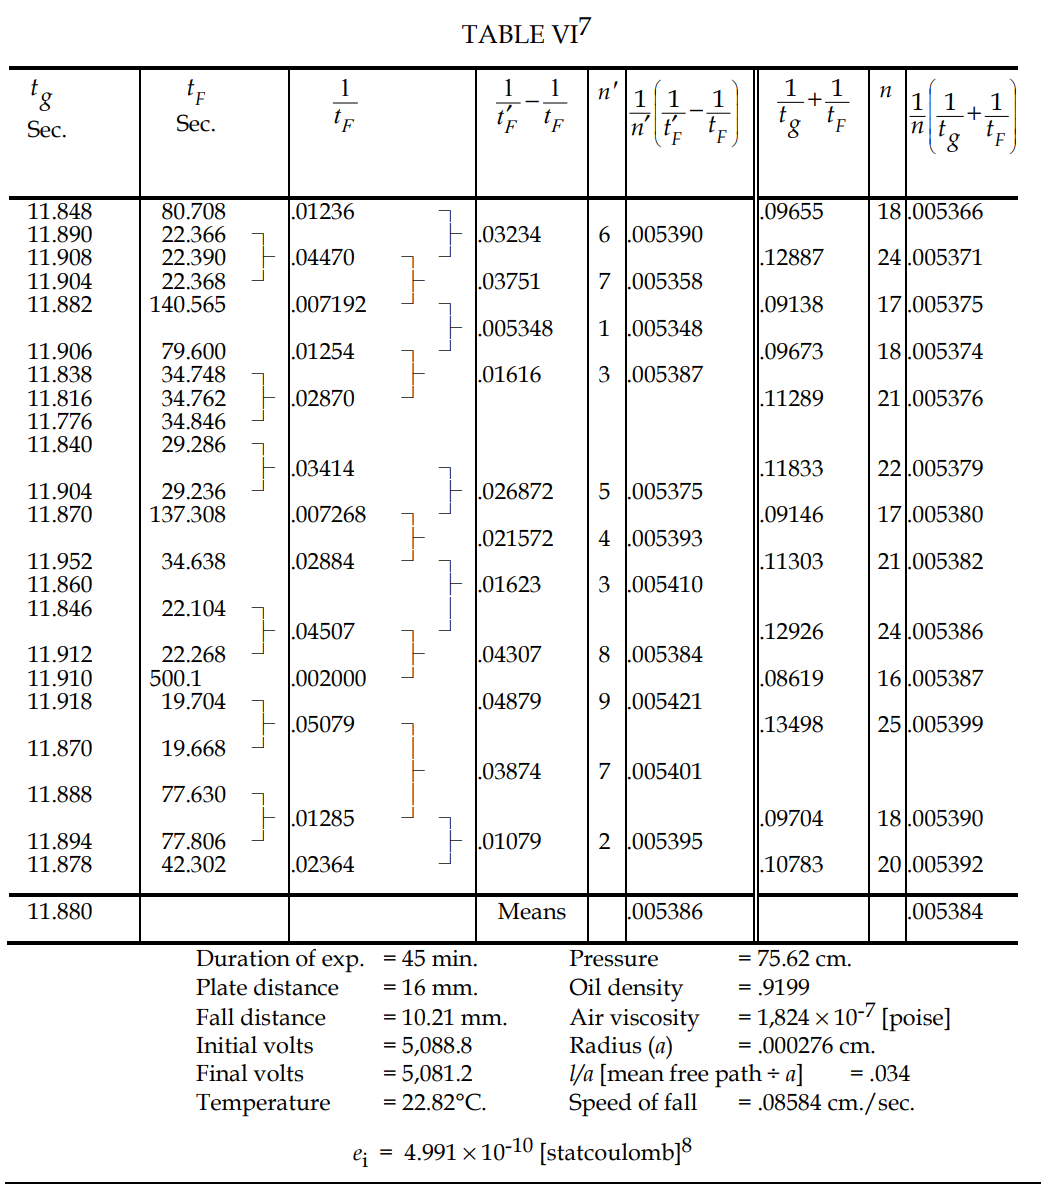
\includegraphics[width=.9\textwidth]{images/03_millikan/table-vi.png}
  \end{center}
\end{figure}
% This is embarrassingly ad hoc: an image of a table I could not figure
% out how to typeset in LaTeX, which included set footnotes. This solution
% is brittle and will not survive if footnotes are added or removed.

\setcounter{footnote}{7}
\footnotetext{[The table entries are given as published; but two
  values are erroneous. In the fourth column, .03874 should be .03794.
  On the same line in the sixth column, .005401 should be .005420. These
  errors do not significantly affect the results.]}

\setcounter{footnote}{8}
\footnotetext{[The value
  presently accepted is $4.802\!\times\!10^-{10}$ statcoulomb.]}

For reasons which will be explained in the next section, each one of
these changes may correspond to the capture of not merely one but of
several distinct ions. The numbers in the fifth column represent simply
the small integer by which it is found that the numbers in the fourth
column must be divided in order to obtain the numbers in the sixth
column. These {[}numbers in the sixth column{]} will be seen to be
exactly alike within the limits of error of the experiment. The mean
value at the bottom of the sixth column represents, then, the smallest
charge ever caught from the air, that is, it is the elementary
\emph{ionic} charge. The seventh column gives the successive values of
$v_1 + v_2$ expressed as reciprocal times. These numbers,
then, represent the successive values of the \emph{total} charge carried
by the droplet. The eighth column gives the integers by which the
numbers in the seventh column must be divided to obtain the numbers in
the last column. These {[}numbers in the last column{]} also will be
seen to be invariable. The mean at the bottom of the last column
represents, then, \emph{the electrical unit out of which the frictional
charge on the droplet was built up, and it is seen to be identical with
the ionic charge represented by the number at the bottom of the sixth
column.}

It may be of interest to introduce one further table (Table VII)
arranged in a slightly different way to show how infallibly the atomic
structure of electricity follows from experiments like those under
consideration.

\begin{center}
\begin{tabular}{c|c|c|c|c|c}
\hline
\multicolumn{6}{c}{TABLE VII}\\
\hline
$n$ & $4.917\!\times\!{n}$ & Observed Charge & $n$ & $4.917\!\times\!{n}$ & Observed Charge\\
\hline
1 & 4.917 & \ldots & 10 & 49.17 & 49.41\\
2 & 9.834 & \ldots & 11 & 54.09 & 53.91\\
3 & 14.75 & \ldots & 12 & 59.00 & 59.12\\
4 & 19.66 & 19.66  & 13 & 63.92 & 63.68\\
5 & 24.59 & 24.60  & 14 & 68.84 & 68.65\\
6 & 29.50 & 29.62  & 15 & 73.75 & \ldots\\
7 & 34.42 & 34.47  & 16 & 78.67 & 78.34\\
8 & 39.34 & 39.38  & 17 & 83.59 & 83.22\\
9 & 44.25 & 44.42  & 18 & 88.51 & \ldots\\
\hline
\end{tabular}
\end{center}

In this table 4.917 is merely a number obtained precisely as above from
the change in speed due to the capture of ions and one which is
proportional in this experiment to the ionic charge. The column headed
4.917 $\times$ \emph{n} contains simply the whole series of exact multiples of
this number from 1 to 18. The column headed ``Observed Charge'' gives
the successive observed values of ($v_1 + v_2$). It will be
seen that during the time of observation, about four hours, this drop
carried all possible multiples of the elementary charge from 4 to 18,
save only 15. \emph{No more exact or more consistent multiple
relationship is found in the data which chemists have amassed on the
combining powers of the elements and on which the atomic theory of
matter rests than is found in the foregoing numbers.}

Such tables as these---and scores of them could be given---place beyond all
question the view that an electrical charge wherever it is found,
whether on an insulator or a conductor, whether in electrolytes or in
metals, has a definite granular structure, that it consists of an exact
number of specks of electricity (electrons) all exactly alike, which in
static phenomena are scattered over the surface of the charged body and
in current phenomena are drifting along the conductor. Instead of giving
up, as Maxwell thought we should some day do, the ``provisional
hypothesis of molecular charges,'' we find ourselves obliged to make all
our interpretations of electrical phenomena, \emph{metallic as well as
electrolytic}, in terms of it.

\subsection*{III. Mechanism of Change of Charge of a Drop}

All of the changes of charge shown in Table IV were spontaneous changes,
and it has been assumed that all of these changes were produced by the
capture of ions from the air. When a negative drop suddenly increases
its speed in the field, that is, takes on a larger charge of its own
kind than it has been carrying, there seems to be no other conceivable
way in which the change can be produced. But when the charge suddenly
\emph{decreases} there is no a priori reason for thinking that the
change may not be due as well to the direct loss of a portion of the
charge as to the neutralization of this same amount of electricity by
the capture of a charge of opposite sign. That, however, the changes do
actually occur, when no X-rays or radioactive rays are passing between
the plates,\footnote{{[}As he elsewhere explains, Millikan repeatedly
  directed x-rays through the chamber or brought radioactive material
  into proximity with it. These measures would greatly accelerate the
  formation of ions in the air and so increase the chances of capturing
  one. But since they might also, by the same token, directly affect the
  charge carried by a droplet, Millikan considers only those changes
  that occur in the absence of such external influences.{]}} only by the
capture of ions from the air, was rendered probable by the fact that
drops not too heavily charged showed the same tendency on the whole to
increase as to decrease in charge. This should not have been the case if
there were two causes tending to decrease the charge, namely, direct
loss and the capture of opposite ions, as against one tending to
increase it, namely, capture of like ions. The matter was very
convincingly settled, however, by making observations when the gas
pressures were as low as 2 or 3 mm. of mercury. Since the number of ions
present in a gas is in general proportional to the pressure,\footnote{{[}That
  the number of \emph{molecules} present in a gas is strictly
  proportional to the pressure, is an element in Avogadro's hypothesis.
  A relatively constant \emph{fraction} of these molecules will become
  ionized under given conditions independent of pressure; hence the
  proportionality cited.{]}} spontaneous changes in charge should almost
never occur at these low pressures; in fact, it was found that drops
could be held for hours at a time without changing. The frequency with
which the changes occur decreases regularly with the pressure, as it
should if the changes are due to the capture of ions. For the number of
ions formed by a given ionizing agent must vary directly as the
pressure.

Again, the changes do not, in general, occur when the electrical field
is on, for then the ions are driven instantly to the plates as soon as
formed, at a speed of, say, 10,000 cm per second, and so do not have
any opportunity to accumulate in the space between them. When the field
is off, however, they do so accumulate until, in ordinary air, they
reach the number of, say, 20,000 per cubic centimeter. These ions, being
endowed with the kinetic energy of agitation characteristic of the
temperature, wander rapidly through the gas and become a part of the
drop as soon as they impinge upon it. It was thus that all the changes
recorded in Table IV took place.\\
\centerline{* * *}
%
\section*{Comment \\
  {\large``Weighing'' the Oil Drop}}

As Millikan shows in his Table V, the two equations
%
\begin{center}
\begin{align*}\tag{9}
\frac{v_1}{v_2} = \frac{mg}{Fe_n-mg} & \: & \text{or} & \: & e_n = \frac{mg}{Fv_1}(v_1+v_2)
\end{align*}
\end{center}
%
and
%
\begin{equation}\tag{10}
e_i = e_{n'}-e_n=\frac{mg}{Fv_1}(v_{2}'-v_2)
\end{equation}
%
suffice to determine \emph{relative} values for $e_n$ (total charge
on an oil drop) and $e_i$ (charge of a captured ion), using nothing
more than stopwatch measurements on the motion of the drop. The
equations will determine \emph{exact} values for those charges as well;
but only if he can evaluate \emph{mg}, the ``effective'' weight of the
drop in a buoyant medium, which we have already expressed above as
%
\begin{equation*}
mg = V(\sigma\!-\!\rho)g
\end{equation*}
%
or, assuming the drop to be a sphere of radius \emph{a},
%
\begin{equation*}\tag{3.6}
mg = \frac{4\pi{a}^3}{3}(\sigma\!-\!\rho)g.
\end{equation*}
%
Millikan has no way to measure this quantity directly; but reasoning
from the viscous (resistive) properties of the medium, air, he is able
to devise an indirect measurement.

We have already derived in equation (3.3) an expression for the limiting 
velocity attained by a body that falls through a viscous medium:
%
\begin{equation*}\tag{3.3}
v_1 = \frac{mg}{R}
\end{equation*}
%
where $R$ is a so far unspecified proportionality constant. This
constant is different for every different-sized oil drop. However,
Millikan was able to relate it to a general, measurable quantity. The
\emph{viscosity} of a fluid is its resistance to being passed through,
as we mentioned, or to flowing past something. This property can be more
precisely defined and measured by various procedures.\footnote{The
  details are beyond our scope.} Accurate tables of the viscosity of air
were available to Millikan. In addition, \emph{Stokes's Law} (derived by
George Stokes in 1845) applies this property to the case of a smooth
sphere moving through a fluid. Millikan assumed that his oil drops were
spheres; with air viscosity $\eta$ and drop radius $a$, Stokes's
Law gives $R = 6\pi \eta a$.\footnote{Again, we cannot follow the
  details.} Substituting into Eq. 3.3) gave Millikan
%
\begin{equation*}\tag{3.7}
v_1 = \frac{mg}{6\pi\eta a}.
\end{equation*}
%
He then eliminated \emph{a} between equations (3.6) and (3.7) to obtain
%
\begin{equation*}
m = \frac{4\pi}{3}(\sigma\!-\!\rho)\left(\frac{mg}{6\pi\eta v_1}\right)^3,
\end{equation*}
%
from which
%
\begin{equation*}
\left(\frac{mg}{v_1}\right)^2 = \frac{3\cdot6^3\pi^2\eta^3{v}_1}{4g(\sigma\!-\!\rho)}.
\end{equation*}
%
Hence for the coefficient $mg/Fv_1$ in Millikan's equations (9) and (10) we have
%
\begin{equation*}\tag{3.8}
\frac{mg}{Fv_1} = \left(\frac{9\pi}{F}\sqrt{\frac{2\eta^3}{g(\sigma\!-\!\rho)}}\right)\cdot\sqrt{v_1}
\end{equation*}
%
which is sufficient to evaluate $e_n$ and $e_i$.

\section*{Experiment: Measurement of the ``Atom of Charge''}

We use the Pasco oil-drop apparatus, which is similar to Millikan's,
only far smaller. In addition, the viewing telescope and associated
illumination are integrally mounted. Make sure that the apparatus is
level, the telescope illumination \emph{on}, and the high voltage
\emph{off}. If the following preliminary adjustments have not already
been made by the laboratory assistant, perform them now:

\emph{Focus the telescope:} Remove the chamber housing, lid, and droplet
hole mask, as illustrated in the drawing. Unscrew the focusing wire from
its storage position and carefully insert it into the droplet hole in
the center of the upper plate. Adjust the Reticle Focusing Ring on the
telescope to bring the viewing reticle into focus. Adjust the Droplet
Focusing Ring to bring the wire image into sharp focus. When the
telescope is focused, each minor reticle division corresponds to a
droplet fall distance of .01 cm; each major division to .05 cm.

\emph{Focus the lamp:} Turn the lamp's Horizontal Adjustment to bring
the right edge of the wire into highest contrast compared to the center
of the wire. Turn the Vertical Adjustment to direct the brightest light
onto the part of the wire that is within the reticle. Remove and return
the focusing wire to its storage position and reassemble the chamber.

\begin{wrapfigure}[18]{r}{2.45in} % this can appear anywhere in this subsection
										  % move if necessary
  \begin{center}
    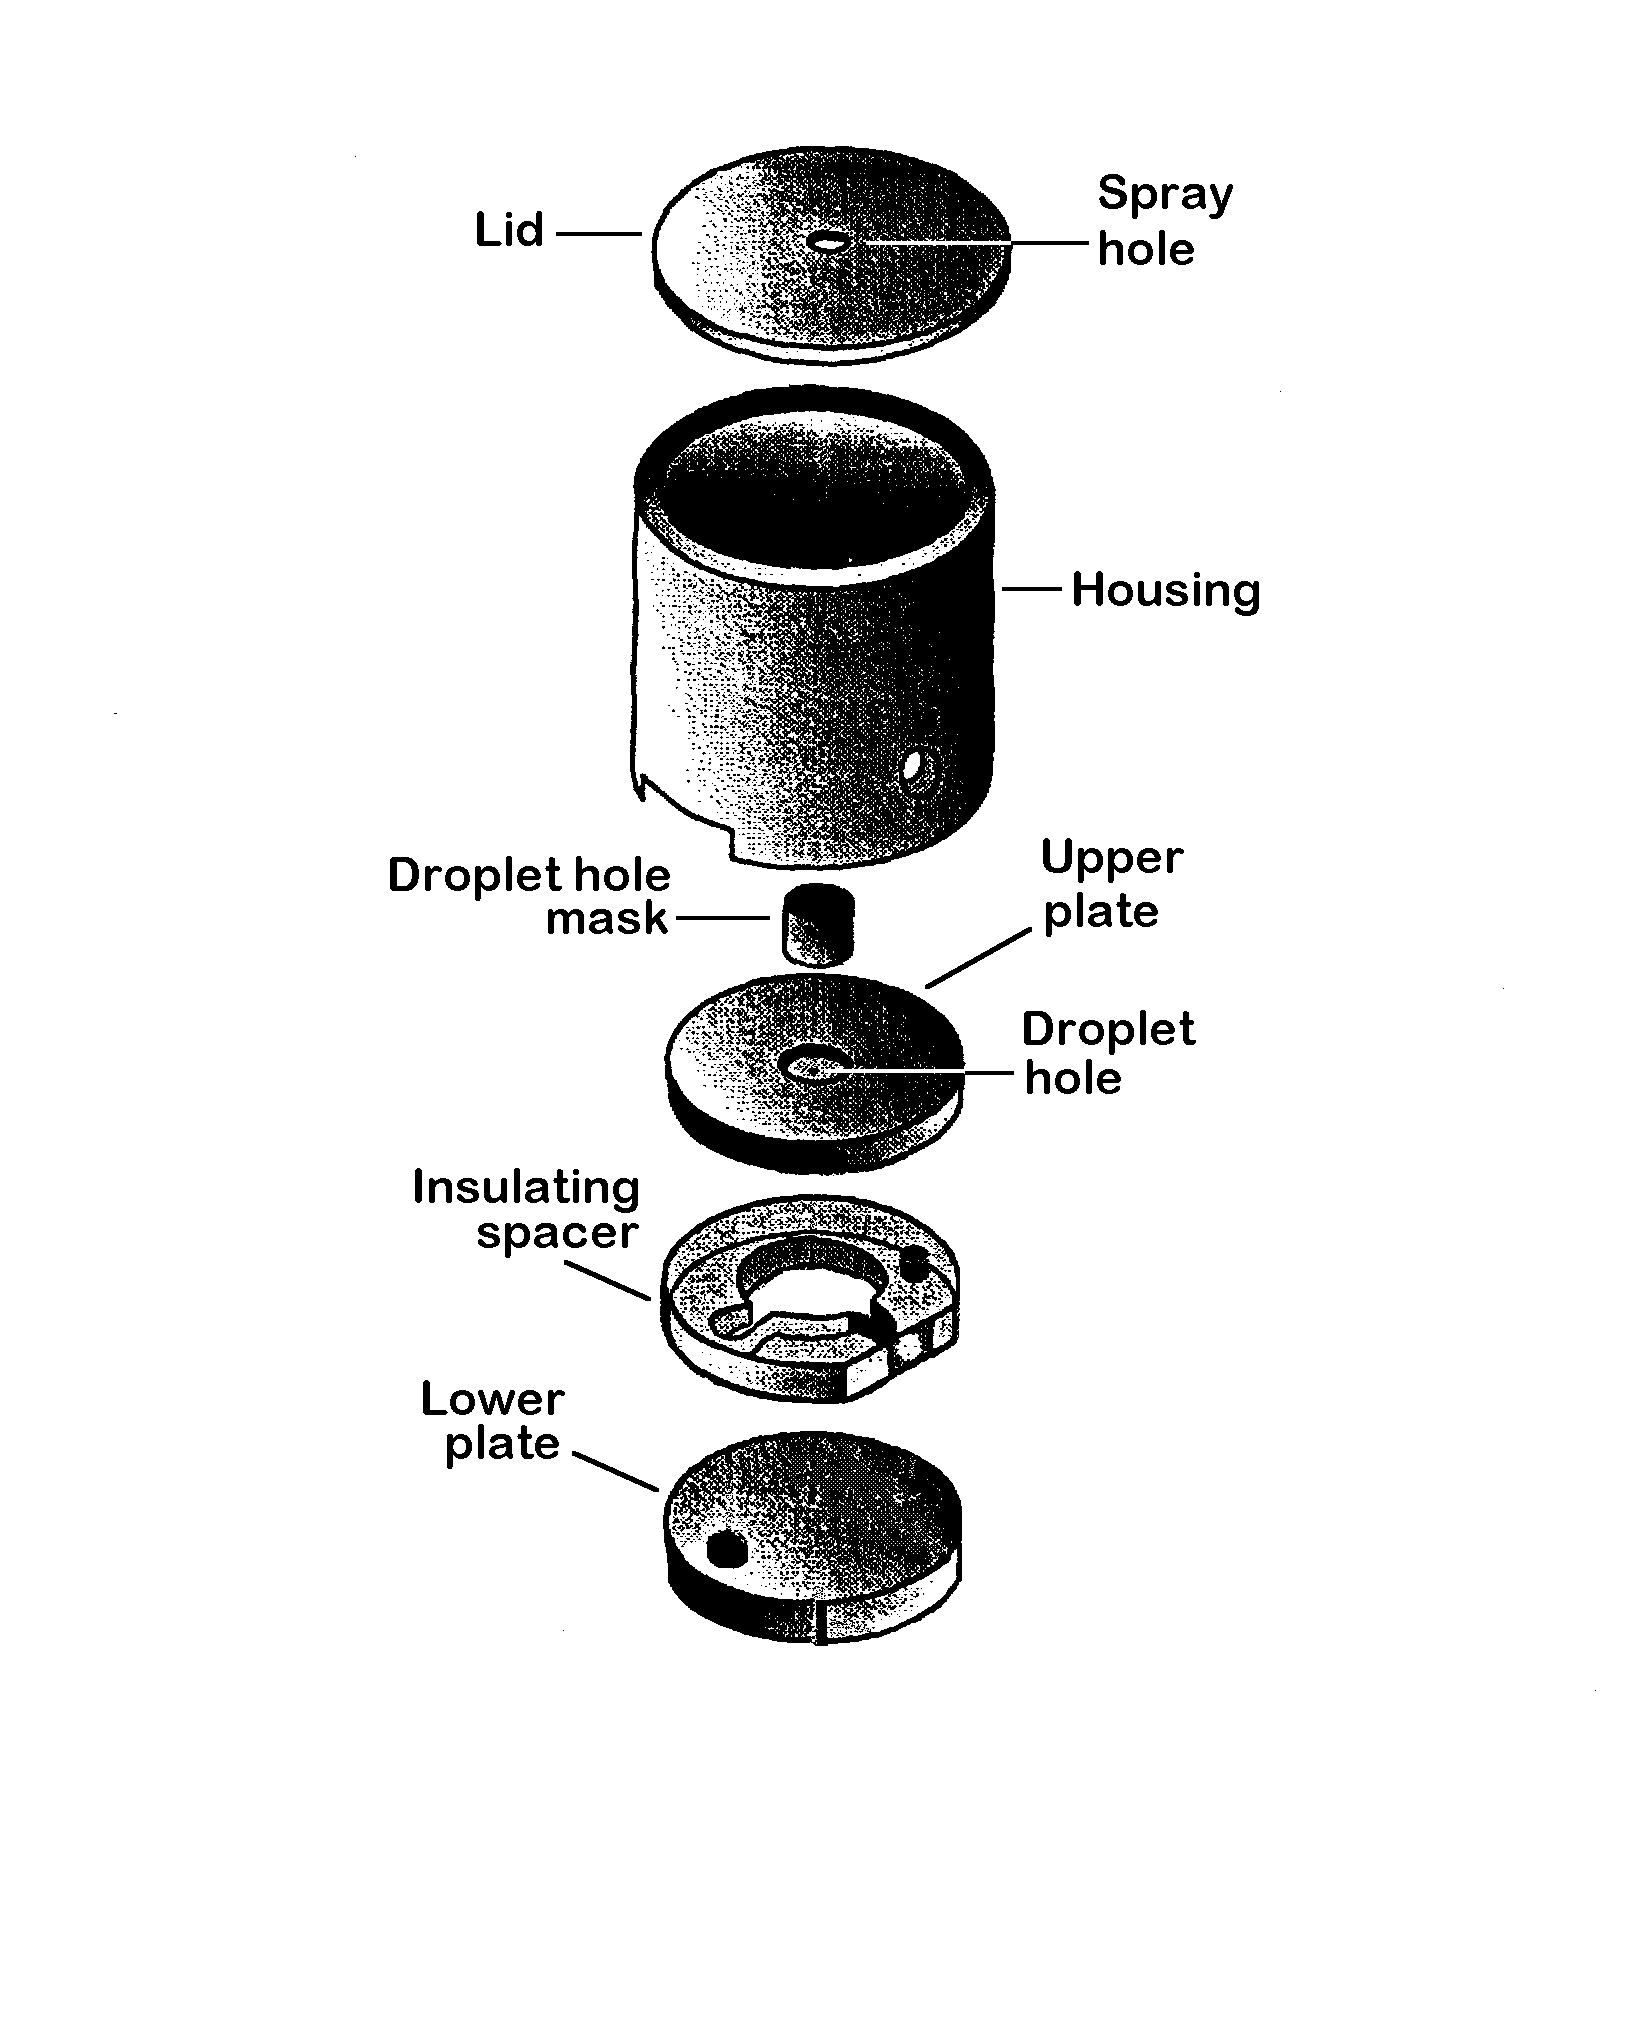
\includegraphics[width=2.33056in,height=3.38264in]{images/03_millikan/image067.png}
  \end{center}
\end{wrapfigure}

\emph{Adjust the plate voltage:} Connect the high-voltage supply. Turn
the cable-mounted plate switch to the GROUNDED position. Adjust the
supply to deliver between 400 and 500 volts, and record the voltage. The
apparatus is now ready for use.

Begin by introducing oil droplets into the chamber. Move the vent lever
to the Spray Droplets position; this will permit air to escape from the
chamber as the oil spray enters. The atomizer nozzle should be turned
vertically downward. After one or two test squeezes to make sure oil
sprays correctly, point the nozzle into the spray hole in the lid of the
chamber.

While looking through the telescope, give the atomizer \emph{one quick
squeeze}, followed im\-me\-di\-ate\-ly by \emph{one slow squeeze} to create a
vertical downdraft. When you see a shower of drops through the
telescope, move the vent lever to the OFF po\-si\-tion.\footnote{Avoid
  immoderate use of the atomizer. The object is to introduce a small
  number of drops, from which a single drop can be chosen. If a large,
  bright cloud appears in the viewing area, spraying has been excessive.
  You can try waiting a few minutes to see if the drops settle out of
  view, but most likely the chamber will have to be disassembled and
  cleaned.}

With a number of drops in view, observe that different drops fall with
noticeably different speeds. This illustrates the relation expressed in
equation (3.3)---heavier drops fall proportionately faster than lighter
ones. Pay attention to those droplets that fall \emph{slowly}---about
10--25 seconds to travel the distance between major reticle lines (.05
cm).

Energizing the plates will reveal which drops bear a charge, and whether
the applied voltage is in the right direction to \emph{reverse} a drop's
falling motion (which is desired) or not. Repeatedly move the
cable-mounted plate switch to its + or -- positions. When a droplet is
found that can be driven back towards the upper plate by applying the
voltage, try to keep it in capture by alternately applying and removing
that voltage.

\subsubsection*{Measurements on a single drop}

Execution of the experiment will require two people, one to observe the
drop and operate the stopwatch, the other to read the watch and record
the timed intervals. It is usually best to time successive rising and
falling transits of the droplet over any \emph{major} (.05 cm) division
on the telescope's viewing reticle---ten to twenty measurements in each
direction are desirable. Do not raise or lower the plate voltage
adjustment once you begin timing a drop. Record the fall times and rise
times in separate columns. A series of measurements of these times,
\emph{all performed on the same drop}, will enable you to construct a
table like Millikan's Table VI. Here is an example (figures are from
1997):

\begin{center}
\small
\begin{tabular}{|l|c||c|c|c|c|c|c|c|c|}
\hline
 & $d$ = 0.5cm & & $d$ = 0.5cm & \makecell{Charge\\on ion} & & & \makecell{Frictional\\charge} & & \\
\hline
$t_g$ & \makecell{$v_1(=d/t_g)$\\(cm/sec)} & $t_F$ & \makecell{$v_2(=d/t_F)$\\(cm/sec)} & $(v_{2}'\!-\!v_2)$ & $n'$ & $\frac{v_{2}'-v_2}{n'}$ & $v_1+v_2$ & $n$ & $\frac{v_1+v_2}{n}$\\
\hline
18.2    & .00286 & 3.8 & 0.01316 & & & & 0.01602 & 3 & .00534\\
18.6    & \emph{avr}  & & & .00470 & 1 & .00470 & & & \\
19.2    & & 2.8 & .01786 & & & & & & \\
18.0    & & & & .01561 & 3 & .00520 & & & \\
17.2    & & 22.2 & .00225 & & & & & & \\
15.4    & & & & .00544 & 1 & .00544 & & & \\
16.7    & & 6.5 & .00769 & & & & & & \\
18.0    & & & & .00541 & 1 & .00541 & & & \\
15.4    & & 21.9 & .00228 & & & & & & \\
17.3    & & & & .01123 & 2 & .00562 & & & \\
\underline{18.4}    & & 3.7 & .01351 & & & \underline{\hspace{2em}} & & & \underline{\hspace{2em}} \\
17.5 & & & & & & .00527 & & & .00534 \\
\emph{avr} & & & & & & \emph{avr} & & &\\
\hline
\end{tabular}
\end{center}

\subsubsection*{Measurements on Multiple Drops}

Although it would be convenient to make all measurements on a single
droplet, it is seldom possible to do so; for it proves extremely
difficult to hold any one drop in play for long periods of time. But
droplets of the same material differ from one another only in mass.
Therefore---see Equation 3.8 above---if the electric field intensity
\emph{F} is not changed, the coefficient in Millikan's equations (9) and
(10) will vary, from drop to drop, only in proportion to $\sqrt{v_1}$. You may
therefore combine data from different drops by tabulating and comparing
\begin{center}
\begin{tabular}{ c c c }
$\sqrt{v_1}(v_1+v_2)$ & and & $\sqrt{v_1}(v_{2}'-v_2)$\\
\end{tabular}
\end{center}
instead of (\emph{v}\textsubscript{1} + \emph{v}\textsubscript{2}) and
(\emph{v}'\textsubscript{2} -- \emph{v}\textsubscript{2}) directly. Here
is an example of such a table (the figures are from 1983):

\begin{center}
\small
\begin{tabular}{l l l l l l}
\hline
Obsvd. $t_g$ & $v_1$ (i.e., $1/t_g$) & Obsvd. $t_F$ & $v_2$ (i.e., $1/t_F$) & $(v'_2-v_2)$ & $\sqrt{v_1}(v'_2-v_2)$\\
\hline
7.2 sec & .1389 & 2.1 sec & .4762 & .1984 & .0739\\
 & & 3.6 & .2778 & .1978 & .0737\\
 & & 12.5 & 0.0800 & &\\
5.8 sec & .1724 & 1.9 & .5263 & .3792 & .1575\\
 & & 6.8 & .1471 & .8529 & .3541\\
 & & 1.0 & 1.000 & .7059 & .2931\\
 & & 3.4 & .2941 & &\\
\end{tabular}
\end{center}

The table entries reflect measurements on two different droplets. In the
sixth column the observed changes in rise speed are multiplied by
$\sqrt{v_1}$ as explained above. The resulting quantities
are very nearly integral multiples of about .076. This trial, therefore,
would indicate the existence of a fundamental ionic charge, with a
relative value of about .076.

\subsubsection*{Enhancing Ionization}

It is hoped that the droplet will acquire an ion during one of its
falls, as is indeed illustrated in the foregoing
chart. Capture of an ion does not change the drop's falling velocity,
but it will change the drop's rising velocity when the plate voltage is
next applied. However, should you find that your droplet has not caught
an ion after 10--20 successive rises, move the vent lever to the
IONIZATION ON position for a few seconds during the next fall period.
That will expose the air in the chamber to a low-level radioactive
thorium source, thus increasing the number of ionized particles in the
air and multiplying the chances for the falling drop to encounter an
ion. Repeat the exposure if again the drop fails to capture an ion after
10-20 measurements, and continue for as long as the droplet can be held
in play. It is desirable to measure as many different charges on a
single drop as possible.

\subsubsection*{Frictional Charge and Ionic Charge}

As Millikan explains, the \emph{initial} charge on a droplet, prior to
the capture of an ion, must have been acquired by friction during the
spraying process. In the foregoing chart it is assumed that the first
measurement made on the drop reflects this initial frictional charge.
While that may be a reasonable assumption provided the first measurement
was made \emph{soon} after spraying, and the observed frequency of ion
capture by a drop is not high, remember that it is \emph{only} an
assumption---the drop may have already picked up an ion by the time we
first measure it. That is especially to be suspected when, as in this
example, the apparent number $n$ of unit charges on the drop is
only \emph{3}---a number so small it could as easily reflect ion capture
as frictional electrification.

If it is desired to measure \emph{frictional charges specifically}, do
not use the ionization source---we want to minimize the chances of
capturing an ion. As soon after spraying as possible, try to select a
drop whose rising velocity is noticeably \emph{faster} than others.
Rapid rising indicates a high charge, which is more likely to have been
frictionally acquired. As before, time the drop for 10--20 transits, or
until it appears to have en\-coun\-tered an ion. Let the drop escape; spray
again, and repeat the measurements on another drop.

\subsubsection*{Calculation of the Fundamental Charge}

The stopwatch measurements illustrated in the previous chart suffice to
determine values of and which, as Millikan's equations (9) and (10) make
clear, are proportional to the \emph{initial frictional charge on a
drop} and the \emph{charge on a captured ion}, respectively. But in
order to calculate exact values of these charges, not just relative
ones, we must evaluate the coefficient that appears in those equations.
By our equation 3.8 above, the coefficient can be calculated
from the following quantities:

\begin{quote}
(a) the velocity $v_1$ of the falling drop. This you have already
measured; just remember to cite the correct value for each different
drop. (Remember to average and to take the square root.)

(b) the electric field intensity $F$ between the plates. To compare our 
results numerically with Millikan's we will calculate this in e.s.u., 
so we must express the potential difference between the
plates in e.s.u., i.e.\ in \emph{statvolts}. Our meters give volts and 1
volt = 1/300 statvolts, so \emph{the voltmeter reading must be divided
by 300}. The plate separation is 0.76 cm, unless a different value is
labeled on the side of your apparatus. Then the voltage in statvolts
divided by the plate separation in cm will give electric field intensity
in e.s.u.\footnote{See Appendix for an explanation of the units and for the
  relation between $F$ and the potential difference.}

(c) the density of the oil, $\sigma$. We use Squibb \#5597 non-volatile
mineral oil, for which $\sigma = .886\ \text{g/cm}^3$.

(d) the density of the air, $\rho$, obtained from the graph below. You
will have to note the temperature of the air in the chamber and the 
barometric pressure in the room. Typical values for
$\rho$ are about $.0012\ \text{g/cm}^3$.

(e) the viscosity of the air, $\eta$, obtained from the graph below.
Typical values for $\eta$ are around $1825\ \times\ 10^{-7}\ \text{poise (gm/cm-sec)}.$

(f) the acceleration of gravity, $g = 980\ \text{cm/sec}^2$.
\end{quote}


\begin{figure}[h]
  \begin{center}
    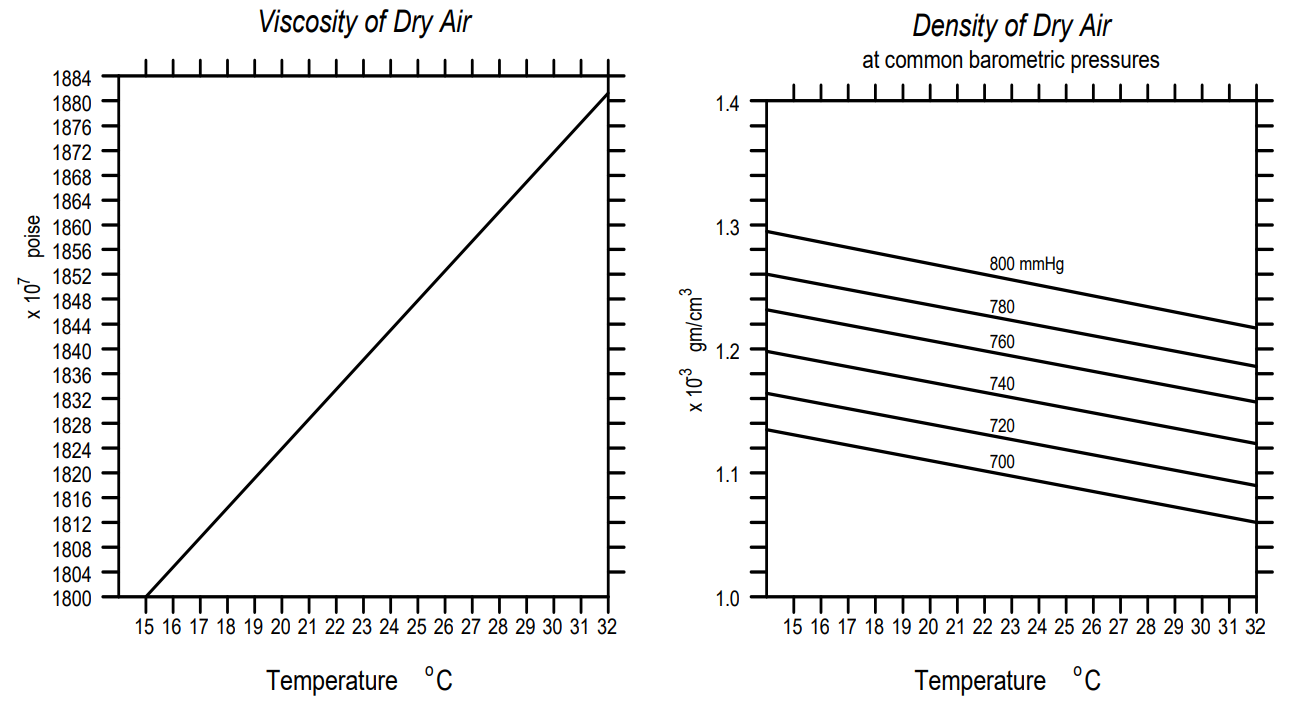
\includegraphics[width=0.9\textwidth]{images/03_millikan/image100.png}
  \end{center}
\end{figure}


%\includegraphics[width=5.53889in,height=3.07847in]{media/image47.wmf}

\subsubsection*{Remarks on Avogadro's Number}

As Millikan himself pointed out, mere \emph{measurement} of the
fundamental charge is not necessarily, in itself, the most important
fruit of this experiment. Of far greater con\-se\-quence, perhaps, is the
demonstration that the same ``electron'' lies at the root of both
\emph{static electricity} (the frictional charge on the drop) and
\emph{chemical activity} (the ionic charge). This is strong, even
conclusive evidence, for the interpretation of chemical power as being
fundamentally electrical, for Millikan's results indicate that the
\emph{fundamental unit of charge} corresponds also to the
\emph{fundamental unit of chemical combining power}. If the electron has
indeed this dual significance, then Millikan's measurement of the
electron charge will at last permit accurate calculation of that
theoretically pivotal but ex\-per\-i\-men\-tal\-ly elusive quantity,
\emph{Avogadro's number}---the number of atoms in a gram-atomic weight
of any element.\footnote{There had been earlier efforts to estimate
  Avogadro's number, predating Millikan's oil-drop measurements;
  Einstein cites one of his own in his paper that appears in Chapter VI
  below. But the most reliable determinations of Avogadro's number and
  many other constants all depend on accurate knowledge of the electron
  charge (cf.\ \emph{The Electron}, Chapter X).}

Recall that the ``equivalent weight'' of an element is that much of it,
measured on the scale of atomic weights with Hydrogen = 1, which
exercises \emph{one unit} of chemical combining power. But the combining
power of one hydrogen atom is taken as the unit for chemical combining
power generally; thus for hydrogen and all atoms equal to hydrogen in
their combining power, the atomic weight and the equivalent weight are
the same.\footnote{Chemical combining power is commonly expressed in
  units of ``valence''; hydrogen and all atoms equivalent to it are said
  to be \emph{univalent} atoms.}

Now if one unit of chemical combining power actually means \emph{one
electron of electric charge}, then one gram-atomic weight of hydrogen
will exercise the cumulative charge of Avogadro's number of electrons,
which is
%
\begin{equation*}
N_0\!\times\!e,
\end{equation*}
%
where $N_0$ denotes Avogadro's number and \emph{e} is the electron
charge. Now the above is also the total charge associated with a
gram-equivalent weight of hydrogen, since for it the gram-atomic weight
is equal to the gram-equivalent weight. But we found in electrolysis
that the total charge associated with liberation or transfer of one
gram-equivalent weight of \emph{any} element is 96,500 coulombs, which
equals $2.895 \times 10^{14}$ stat\-cou\-lombs; hence we may write
%
\begin{equation*}
2.895 \times 10^{14} \text{ statC} = N_0\!\times\!e
\end{equation*}
%
While Millikan has shown that (modern value):
\begin{equation*}
e = 4.802\!\times\!10^{-10} \text{ statC}
\end{equation*}
Thus we have
\begin{equation*}
N_0 = \text{Avogrado's number} = \frac{2.895\!\times\!10^{14}}{4.802\!\times\!10^{-10}} = 6.028\!\times\!10^{23}.
\end{equation*}
(Other, more recent, determinations yield $6.023\!\times\!10^{23}$.)

\subsubsection*{Weighing and Sizing Elementary Particles}

Determination of Avogadro's number puts us in a position to ``weigh all
the atoms''; for if there are $N_0$ atoms in a gram-atomic weight of
an element, then each atom must weigh $1/N_0$ of the gram-atomic
weight. For example, a gram-atomic weight of hydrogen weighs 1.008
grams. Then a single hydrogen atom, for example, must weigh
\begin{equation*}
1.008 \div (6.023\!\times\!10^{23}) = 1.674\!\times\!10^{-24} \text{ g}
\end{equation*}
and similarly for all the other atoms.

In Chapter II of \emph{The Electron} Millikan pointed out that the term
``electron'' had been first introduced in 1891 as a name for the
supposed ``natural unit of electricity,'' namely, that quantity of
electricity exhibited by a hydrogen ion or any other univalent ion. Thus
it denoted simply a \emph{definite quantity of electricity} without
reference to any mass or inertia which might be associated with it. It
is clear that Millikan's oil-drop experiment has proved the existence of
``electron'' in this original sense.

But measurements by Thomson and others of the charge-to-mass ratio of
ions in both gases and liquids strongly implicated Thomson's
\emph{cathode-ray corpuscle} as the es\-sen\-tial constituent whereby atoms
acquire either an excess or deficiency of negative charge to become
ions.\footnote{See note 5 above; Millikan devotes the whole of
  his Chapter II to this very interesting story.} This implies that
\emph{the charge borne by each cathode ray corpuscle must be the very
quantity of charge that had been termed ``electron.''} As a result,
Millikan explains, the word ``electron'' gradually changed its meaning
to become synonymous with the cathode-ray corpuscle: a particle having
definite mass as well as charge, a constituent not only of cathode rays
but of atoms themselves.\footnote{Millikan views this alteration of
  usage with real distress: ``It is unfortunate that modern writers have
  not been more careful to retain the original significance of
  {[}`electron'{]}, for it is obvious that a word is needed which
  denotes merely the elementary unit of electricity and has no
  implication as to where that unit is found, to what it is attached,
  with what inertia it is associated, or whether it is positive or
  negative in sign.''} Since the electron (in the new sense of
\emph{particle}) has the charge-to-mass ratio that was determined for
cathode-rays, and has, on the other hand, the quantity of charge that is
disclosed in Millikan's experiment, we are able to calculate its mass,
to ``weigh'' the electron itself.

We have, from the cathode rays,
\begin{equation*}
m/e = .5685 \times 10^{-7} \text{g/abC} = 1.895 \times 10^{-18} \text{ g/statC}.
\end{equation*}
Then, since the electron charge is
\begin{equation*}
e = 4.802 \times 10^{-10} \text{ statC},
\end{equation*}
we may calculate
\begin{equation*}
m = 1.895 \times 10^{-18} \times 4.802 \times 10^{-10} = .9099 \times 10^{-27} \text{ g}.
\end{equation*}
Hence the electron will be almost 1840 times lighter than the hydrogen
atom. That an electron weighs such a slight fraction of even the
lightest atom will prove important in formulating a conception of the
atom's structure, as discussed in Rutherford's paper which follows.

\subsubsection*{``Sizing'' an Atom}

Another magnitude interesting in itself and also important in
Rutherford's paper is the approximate \emph{size} of an atom. Using
Avogadro's Number this is easy to calculate for elemental solids.

Take gold, which is what Rutherford will be dealing with. The density of
gold is 19.3 g/cm\textsuperscript{3}, while its gram-atomic weight is
197. Therefore there are .098 gram equivalents in a cubic centimeter of
gold. But since there are $N_0$ atoms in a gram-atomic weight of an
element, we can now say that there are $.098 \times (6.023 \times 10^{23})$, or $5.90 \times
10^{22}$, atoms in a cubic centimeter of gold. Each atom
thus occupies a volume of $1/(5.90 \times 10^{22}) = 1.69 \times
10^{-23}$ cubic centimeters. The cube root of this, $2.57 \times
10^{-8}$ cm, will give the side of a cube of this volume.
Let us assume that gold atoms are spherical and that in solid gold they
fit together in a more or less cubical pattern. Then half of $2.57 \times
10^{-8}$ cm, i.e.\ 
\begin{equation*}
1.285 \times 10^{-8} \text{ cm},
\end{equation*}
is a reasonable rough estimate for the radius of a gold atom. Rutherford
implicitly adopts this size estimate as he analyses how particles that
are \emph{much smaller} than this interact with gold atoms.

\chapter{The Scattering of $\alpha$ and $\beta$ Particles by Matter and the Structure of the Atom}

\chapterprecis{Ernest Rutherford}

\makeoddhead{myheadings}{\emph{Rutherford}}{}{\thepage}
\makeevenhead{myheadings}{\thepage}{}{\emph{The Scattering of $\alpha$ and $\beta$ Particles}}

\section*{Remarks}

We have seen how the ``electron'' may be understood as a charged
particle, bearing the fundamental quantity of negative charge, with a
fixed mass that is far smaller than the lightest of atoms. The chemical
or atomic analysis of matter is thus extended to disclose the prospect
of subatomic constituents having both mass and charge.

Accordingly, physics is challenged to interpret the chemical elements as
more or less complex systems of the primordial constituents. How then,
in the atom, are these constituents distributed with respect to one
another? In 1902 Lord Kelvin proposed a model of an electrically neutral
atom containing both positive and negative charge. The positive charge,
and most of the atom's mass, were in this view distributed continuously
throughout the spherical volume of the atom; while the electrons, which
carry negative charge, were embedded in the sphere of positive charge.
Thomson proceeded to investigate this arrangement both mathematically
and experimentally, and it was eventually named after him. The strongest
argument in favor of the Thomson model was that it seemed to explain the
permanence and stability of atoms: Because the electrons were everywhere
surrounded by equal quantities of positive charge the atom would be
electrically neutral in all its parts. A great deal of energy would then
be required to disturb its equilibrium.

Rutherford initially accepted the essential correctness of Thomson's
scheme and set out to verify it experimentally. He and his associates
Geiger and Marsden proposed to bombard individual gold atoms (in fine
gold foils only about 2000 atoms in thickness) with streams of a
radioactive by-product called \emph{alpha particles}. Two kinds of
particles, distinguished as \emph{alpha} and \emph{beta}, are emitted
spontaneously at very high speeds by radium and other radioactive
materials; beta particles were subsequently identified as high-speed
electrons, while the alpha particles proved to be doubly-charged Helium
ions.\footnote{That is, Helium atoms bearing a charge of +2$e$. A
  Helium \emph{ion} is very anomalous from the viewpoint of chemistry,
  for on the electro-chemical interpretation an ion is a
  \emph{chemically active atom}. But Helium is never chemically active!
  The process that produces alpha-particles, then, must involve aspects
  of the atomic structure that chemistry never touches. Furthermore,
  from measurements of their mean free path it
  looked as though $\alpha$-particles were \emph{far smaller} than
  neutral Helium atoms. It takes Rutherford's theory itself to give an
  explanation for this.} Because of their speed and mass alpha-particles
made suitable ``probes'' with which to explore the interior structure of
atoms. By studying the deflections such particles suffered in passing
through gold atoms, Rutherford expected to obtain a more detailed
picture consistent with the Thomson model.

The experiments yielded results that were wholly unexpected. Since the
highest concentrations of mass in the Thomson model are the
\emph{electrons}; and since these are far lighter than alpha particles
and moreover relatively free to move, it was not to be imagined that a
gold atom should be capable of disturbing the path of an alpha particle
by more than a fraction of a degree. But in fact, prodigious deviations
were observed, some greater than $90^\circ$. And these deflections occurred,
moreover, with a frequency some 104596 times greater than the
probability as calculated according to Thomson's arrangement.
Rutherford, later in life, expressed his astonishment as follows:

\begin{quote}
It was quite the most incredible event that ever happened to me in my
whole life. It was as incredible as if you fired a 15-inch shell at a
piece of tissue paper and it came back and hit you. On consideration I
realized that the scattering backwards must be the result of a single
collision, and when I made the calculation I saw that it was impossible
to get anything of that order of magnitude unless you took a system in
which the greater part of the mass of the atom was concentrated in a
single nucleus. It was then that I had the idea of an atom with a minute
massive center carrying a charge.
\end{quote}

\subsection*{A Note on Probability\footnote{Note by Michael Comenetz}}

A reader of Ernest Rutherford's famous paper \emph{The Scattering of $\alpha$
and $\beta$ Particles by Matter and the Structure of the Atom}, which reports
the discovery of the atomic nucleus, may be perplexed by a couple of
expressions at the beginning of §3. An explanation follows.

\begin{figure}[h]
  \begin{center}
    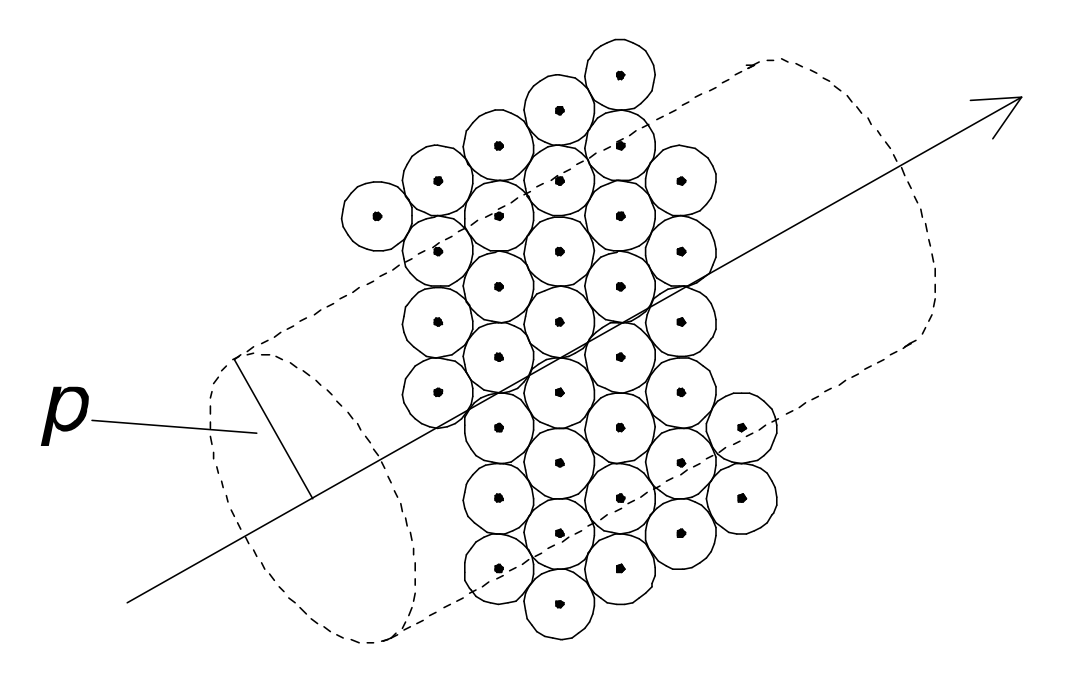
\includegraphics[width=2.1875in,height=1.57292in]{images/04_rutherford/collisions.png}
  \end{center}
    \caption*{\emph{An alpha particle and its presumptive path
      through a section of gold foil. You should imagine the atomic centers 
      as being more randomly arrayed.}}
\end{figure}

We are playing a game of shooting tiny particles at a thin screen of
large spherical atoms, in the direction normal (perpendicular) to its
surface. With very few exceptions, the particles pass straight through
the screen; for our present purpose we assume that all do. Having chosen
a distance $d$, we say that a particle \emph{hits} an atom if it
comes within that distance of the center of the atom. For a given shot,
our \emph{score} is the number of atoms hit by the particle. Each shot
is taken in the same way, and the shots are independent of one
another---the score for one shot has no influence on the score for
another.

When we take a number of shots, our \emph{average score} means the
result of dividing the total of our scores by the number of shots. For
example, if we score successively 2, 0, 5, 2, 0, 2, 3, our total score
is 14 and the number of shots is 7, so our average score~is 2. If we
score successively 1, 0, 0, 0, 1, 0, 1, 0, our total score is 3 and the
number of shots is 8, so our average score~is 0.375.

Since the shots are alike and independent, it is reasonable to suppose
that as we take more and more of them, our average score will approach
some definite value as a limit. The limiting value can be called our
\emph{expected score}, or \emph{expectation}, because when we play the
game, we expect our scores to cluster around that value, and our average
score to tend towards it. The expectation, which we call $e$, will
be well approximated by the average score we get when we take a large
number of shots.

In order to estimate the expectation, let us call the thickness of the
screen $t$, and the density of atoms within it $N$. The latter
quantity means the average number of atoms per unit volume; that is the
same as the average number of centers of atoms per unit volume.

The question, ``On average, how many atoms does a particle hit?'' is
equivalent to the question, ``On average, how many atom-centers lie
within distance $d$ of the path of the particle?'' and therefore
also to the question, ``On average, how many atom-centers lie within the
right circular cylinder of radius $d$ whose axis is the path of the
particle through the screen, and whose height is the thickness $t$
of the screen?''

The volume of such a cylinder---that is, the number of unit volumes it
contains---is the area of its base, which is
$\pi d^2$, times its height $t$, or
$\pi d^{2}t$. It follows that the average
number of atom-centers in such a cylinder is
$n \times \pi d^{2}t = \pi d^{2}nt$. This is then our
expectation: $E = \pi d^{2}nt$

We now apply this result to two special cases.

\textbf{Case 1.}~ Let $d$ be the radius $R$ of an atom. In
this case, \emph{hitting} an atom has the ordinary sense of coming into
contact with it. The expectation $e$ is
$\pi R^{2}nt$. This is what
Rutherford means by saying that ``the number of collisions of the
particle with the atom of radius $R$ is
$\pi R^{2}nt$.'' The value of
$e$ is of the order of the number of atoms spanning the thickness
$t$---a few thousand, for a gold-foil screen.

\textbf{Case 2.}~ Let $d$ be a distance $p$ much smaller than
$R$, a thousand or ten thousand times smaller. In this case it is
very difficult to \emph{hit} an atom---so difficult, that we may assume
that no particle hits more than one. Then for each shot our score is 0
or 1, and the expectation $E = \pi p^{2}nt$ has a value between 0
and 1.

Since in this case there are only two possibilities for each shot,
either it hits or it doesn't, we can speak of the \emph{probability}
$p$ that a given shot will hit an atom, understanding by this the
proportion of hits, or average score, obtained when a great many shots
are taken (more precisely, its limiting value as the number of shots
increases)---that is, the expectation: $p$ = $e$. If we
assert, for example, that $p$ = 0.20, or 20\%, we expect that out
of, say, 1000 shots, there will be about 200 hits---that the average
score for those 1000 shots will be about 200/1000 = 0.20, that about
20\% of them will be hits. Hence Rutherford writes, ``The probability
\ldots{} of entering an atom within distance $p$ of its centre is
given by \ldots{} $\pi p^{2}nt.$''\footnote{See page~\pageref{eq_s:rutherford}.}

\subsection*{Final Thoughts}

1. The assumption in the first paragraph of the explanation is
justified as follows. A particle deviates appreciably from a straight
path only if it hits an atom for very small $d$, as in Case 2. Even
if so deflected, it is very unlikely to hit another atom, because
$d$ is much less than $R$ and $t$ is very small. Thus
only the possibility of a first encounter along a straight path need be
admitted.

2. One may wonder why probability enters the picture only with Case 2.
Shouldn't the general case somehow involve probability? It does. Let
$N$ be the greatest number of atoms the particle can possibly hit.
Let $p_0$ be the probability that it hits no atoms,
$p_1$ the probability that it hits exactly one,
$p_2$ the probability that it hits exactly two,
\ldots{}, \emph{P\textsubscript{N}} the probability that it hits exactly
$N$. Then $p_0$ + $p_1$ +
$p_2$ + $\cdot \cdot \cdot$ + $P_N$ = 1 and
$p_0$ $\cdot$ 0 + $p_1$$\cdot$1 +
$p_2$$\cdot$2 + $\cdot \cdot \cdot$
+~\emph{P\textsubscript{N}}$\cdot$$N$ = $e$. In Case 2, the only
non-zero probabilities are $p_0$ and
$p_1$, hence $p_1$ = $e$.

3. The intuitive understanding of expectation as the limit of the
average score rests on the assumption stated in the third paragraph,
that the limit exists. In the mathematical theory of probability a
different approach is taken, and the limit assertion becomes a theorem,
or rather a class of theorems (\emph{laws of large numbers}).


\section*{The Scattering of $\alpha$ and $\beta$ Particles by Matter\\
  and the Structure of the Atom\footnote{{[}\emph{Philosophical Magazine}
  \textbf{211} (1911), 669--688.{]}}\\
  {\large Ernest Rutherford}}



\S1.\ It is well known that the $\alpha$ and $\beta$ particles suffer
deflexions from their rectilinear paths by encounters with atoms of
matter. This scattering is far more marked for the $\beta$~than for the
$\alpha$~particle on account of the much smaller momentum and energy of
the former particle. There seems to be no doubt that such swiftly moving
particles pass through the atoms in their path, and that the deflexions
observed are due to the strong electric field traversed within the
atomic system. It has generally been supposed that the scattering of a
pencil of $\alpha$~or $\beta$~rays in passing through a thin plate of
matter is the result of a multitude of small scatterings by the atoms of
matter traversed. The observations, however, of Geiger and Marsden on
the scattering of $\alpha$~rays indicate that some of the $\alpha$
particles must suffer a deflexion of more than a right angle in a single
encounter. They found, for example, that a small fraction of the
incident $\alpha$~particles, about 1 in 20,000, were turned through an
average angle of 90$^\circ$ in passing through a layer of gold-foil about
.00004 cm. thick, which was equivalent in stopping-power of the
$\alpha$~particle to 1.6 millimetres of air. Geiger showed later that
the most probable angle of deflexion for a pencil of $\alpha$ particles
traversing a gold-foil of this thickness was about 0$^\circ$.87.\footnote{{[}That
  is, particles passing through the foil were deflected within, say, .1$^\circ$
  of 0.87$^\circ$ more often than within .1$^\circ$ of any other angle.{]}} A simple
calculation based on the theory of probabilities shows that the chance
of an $\alpha$~particle being deflected through 90$^\circ$ {[}as the cumulative
result of multiple encounters{]} is vanishingly small.\footnote{{[}If
  $\theta_0$ is the most probable angle of deflection resulting from many
  atomic encounters, a general theorem holds that the probability of
  obtaining a deflection angle of any other value $\theta$~or greater is
  $e^{-(\theta/\theta_0)^2}$. Since Geiger has shown that $\theta_0 = .87^{\circ}$, the probability of
  obtaining $\theta = 90^\circ$ will be or about $10^-{4600}$.{]}} In addition, it
will be seen later that the distribution of the $\alpha$ particles for
various angles of large deflexion does not follow the probability law to
be expected if such large deflexions are made up of a large number of
small deviations. It seems reasonable to suppose that the deflexion
through a large angle is due to a single atomic encounter, for the
chance of a second encounter of a kind to produce a large deflexion must
in most cases be exceedingly small. A simple calculation shows that the
atom must be the seat of an intense electric field in order to produce
such a large deflexion at a single encounter.

Recently Sir J.\ J.\ Thomson has put forward a theory to explain the
scattering of electrified particles in passing through small thicknesses
of matter. The atom is supposed to consist of a number $N$ of
negatively charged corpuscles, accompanied by an equal quantity of
positive electricity uniformly distributed throughout a sphere. The
deflexion of a negatively electrified particle in passing through the
atom is ascribed to two causes---(1) the repulsion of the corpuscles
distributed through the atom, and (2) the attraction of the positive
electricity in the atom. The deflexion of the particle in passing
through the atom is supposed to be small, while the average deflexion
after a large number $m$ of encounters was taken as
$\sqrt{m} \cdot \theta$, where $\theta$ is the average deflexion due to a
single atom. It was shown that the number $N$ of the electrons
within the atom could be deduced from observations of the scattering of
electrified particles. The accuracy of this theory of compound
scattering was examined experimentally by Crowther in a later paper. His
results apparently confirmed the main conclusions of the theory, and he
deduced, on the assumption that the positive electricity was continuous,
that the number of electrons in an atom was about three times its atomic
weight.

The theory of Sir J.~J. Thomson is based on the assumption that the
scattering due to a single atomic encounter is small, and the particular
structure assumed for the atom does not admit of a very large deflexion
of an $\alpha$ particle in traversing a single atom, unless it be
supposed that the diameter of the sphere of positive electricity is
minute compared with the diameter of the sphere of influence of the
atom.

Since the $\alpha$ and $\beta$ particles traverse the atom, it should
be possible from a close study of the nature of the deflexion to form
some idea of the constitution of the atom to produce the effects
observed. In fact, the scattering of high-speed charged particles by the
atoms of matter is one of the most promising methods of attack of this
problem. The development of the scintillation method\footnote{{[}The
  \emph{scintillation method}: an alpha-particle is made to strike a
  zinc sulphide screen, which then gives off a tiny flash of light. The
  flash is observed with a microscope, and the number of particles
  incident on any given area in a given time interval are thus
  counted.{]}} of counting single $\alpha$ particles affords unusual
advantages of investigation, and the researches of H. Geiger by this
method have already added much to our knowledge of the scattering of
$\alpha$ rays by matter.

\smallskip

\S2.\ We shall first examine theoretically single encounters\footnote{The
  deviation of a particle through a considerable angle from an encounter
  with a single atom will in this paper be called ``single'' scattering.
  The deviation of a particle resulting from a multitude of small
  deviations will be termed ``compound'' scattering.} with an atom of
simple structure, which is able to produce large deflexions of an
$\alpha$~particle, and then compare the deductions from the theory with
the experimental data available.

Consider an atom which contains a charge $\pm Ne$ at its centre
surrounded by a sphere of electrification containing a charge $\mp Ne$
supposed uniformly distributed throughout a sphere of radius $R$.
$e$ is the fundamental unit of charge, which in this paper is taken
as $4.65 \times  10^{-10}$ \textsc{e.s.} unit. We shall suppose that for distances
{[}greater{]}\footnote{{[}We here correct a typographical error in the
  original.{]}} than $10^{-12}$ cm. the central charge and also the charge on
the~$\alpha$ particle may be supposed to be concentrated at a point. It
will be shown that the main deductions from the theory are independent
of whether the central charge is supposed to be positive or negative.
For convenience, the sign will be assumed to be positive. The question
of the stability of the atom proposed need not be considered at this
stage, for this will obviously depend upon the minute structure of the
atom, and on the motion of the constituent charged parts.

In order to form some idea of the forces required to deflect an
$\alpha$~particle through a large angle, consider an atom containing a
positive charge $Ne$ at its centre, and surrounded by a
distribution of negative electricity $Ne$ uniformly distributed
within a sphere of radius $R$. The electric {[}field{]} \emph{X}
and the potential $V$ at a distance $R$ from the centre of an
atom, for a point inside the atom, are given by\footnote{{[}Rutherford's
  actual expression is ``electric force $X$.'' But what he is
  actually calculating is the \emph{intensity} of the force---the force
  per unit charge---and thus $X$ really represents \emph{electric
  field strength}. See Appendix, page~\pageref{ch_sec:appendix}.
  
  [The atom is assumed to contain $N$ negative electrons evenly
  distributed throughout its volume and $N$ positive charges
  concentrated in the nucleus. Thus the electric field within the atom
  at a distance $r$ from the nucleus has two sources: (a) the
  nucleus, and (b) those electrons that are contained \emph{within}
  radius $r$. (Electrons lying \emph{beyond} radius $r$ make
  no contribution to the field at $r$, for the electric field
  within any closed, charged surface is \emph{zero}; compare the
  analogous case for gravitation, Newton's \emph{Principia}, Book I,
  Prop.\ 70.)
  
  [Now (a) the electric field intensity due to the positive nucleus is
  $Ne/r^2$. And the negative charge contained within radius
  $r$ is to $Ne$ as the volume of the sphere of radius
  $r$ is to the whole atom; hence that charge is
  $-Ne(r^3/R^3)$. It acts as though it were
  concentrated at the center (see \emph{Principia}, Book I, Prop.\ 71);
  therefore (b) its contribution to the electric field intensity is
  $-Ne(r^3/R^3)/r^2$ or $-Ne(r/R^3)$. The total electric field intensity
  $X$ is the sum of (a) and (b), as in Rutherford's expression.{]}}
\begin{align*}
X &= Ne\left(\frac{1}{r^2} - \frac{r}{R^3}\right)\quad \text{[and]\footnotemark}\\
V &= Ne\left(\frac{1}{r} - \frac{3}{2R} + \frac{r^2}{2R^3}\right).
\end{align*}
\footnotetext{[To determine the electric potential we
  \emph{integrate} the field strength $X$ \emph{over distance} (again see
  Appendix, p.~\pageref{ch_sec:appendix}, for a discussion of this), from $s = r$ 
  to $s = R$ (it is not necessary to consider radii
  greater than $R$ because, the atom as a whole being electrically
  neutral, there is no field beyond $R$). Thus Rutherford's
  expression for $V$ is the result of having evaluated the integral
  $\int_{r}^{R} \! Ne(1/s^2 - s/R^3)\,ds$.]}%
Suppose an $\alpha$~particle of mass $m$ and velocity $u$\label{uRuth} and
charge $e$ shot directly towards the centre of the atom. It will be
brought to rest at a distance $b$ from the centre given
by\footnote{{[}The work required to bring a positive charge $e$
  from infinity to a distance $r$ from the center of the atom is
  given by the product $VE$ of the charge and the electric
  potential at the distance $r$---again see Appendix. If this
  work is done at the expense of the incident particle's kinetic energy,
  the particle will be brought to rest (at distance $b$ from the
  center) when the initial kinetic energy of the particle equals
  \emph{VE}, that is, when
  \begin{equation*}
  \frac{1}{2}mu^2 = VE = NeE\left(\frac{1}{b}-\frac{3}{2R}+\frac{b^2}{2R^3}\right).]
  \end{equation*}}

\begin{equation*}
\frac{1}{2}mu^2 = NeE\left(\frac{1}{b} - \frac{3}{2R} + \frac{b^2}{2R^3}\right).
\end{equation*}
It will be seen that $b$ is an important quantity in later
calculations. Assuming that the central charge is 100$e$, it can be
calculated that the value of $b$ for an $\alpha$~particle of
velocity $2.09 \times 10^9$ cm. per second is about $3.4 \times 10^{-12}$ cm. In this
calculation $b$ is supposed to be very small compared with
$R$. Since $R$ is supposed to be of the order of the radius of
the atom, viz.\ $10^{-8}$ cm., it is obvious that the $\alpha$~particle before
being turned back penetrates so close to the central charge, that the
field due to the uniform distribution of negative electricity may be
neglected. In general, a simple calculation shows that for all
deflexions greater than a degree, we may without sensible error suppose
the deflexion due to the field of the central charge alone.\footnote{{[}Since
  Rutherford has concluded that $b$ ($\approx 10^{-12}$ cm.)
  is very small in comparison with $R$ ($\approx 10^{-8}$
  cm.), he ignores the last two terms in parentheses in the equation
  above; thus
  \begin{equation*}
  b = 2NeE/mu^2
  \end{equation*}
  This is equivalent to assuming that the electric potential $V$ at
  $b$ was equal to $Ne/b$ and thus that it was due to the
  field of the central charge alone. Rutherford will make use of this
  expression for $b$ below.]} Possible single deviations 
  due to the negative electricity, if distributed in the form
of corpuscles, are not taken into account at this stage of the theory.
It will be shown later that its effect is in general small compared with
that due to the central field.
%
\begin{figure}[htp]
\centering
  %\begin{center}
    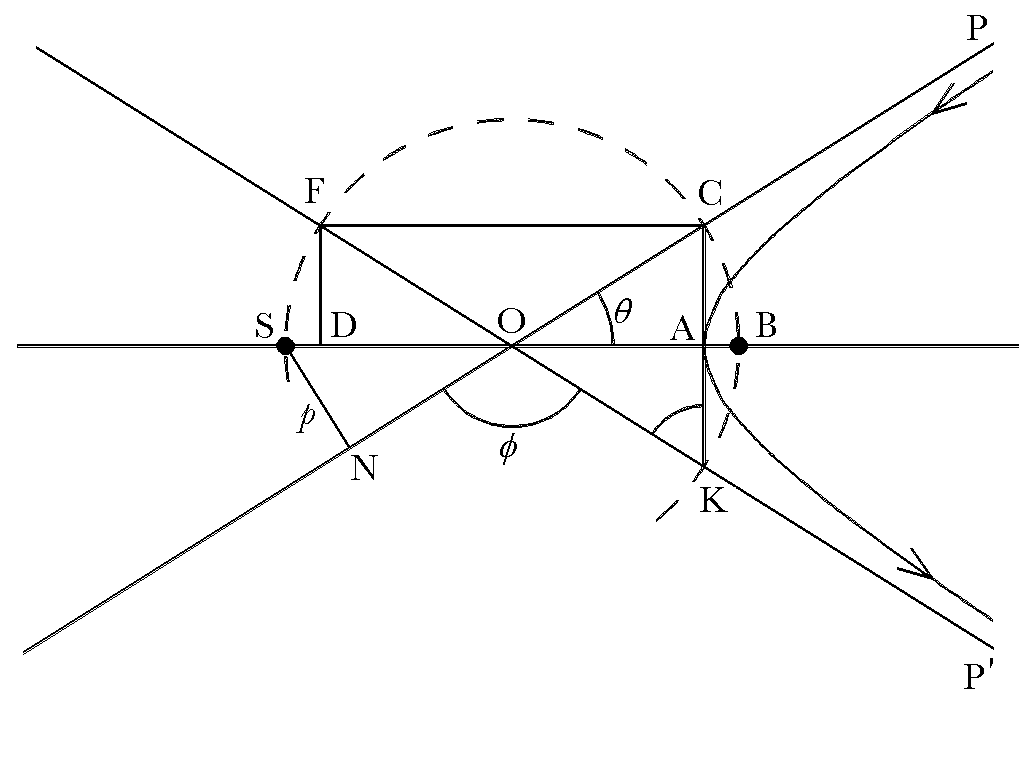
\includegraphics[width=4.65625in,height=3.5in]{images/04_rutherford/image005.png}
  %\end{center}
    \vspace*{-15mm}\caption*{Figure 1}
\end{figure}
%

Consider the passage of a positive electrified particle close to the
centre of an atom. Supposing that the velocity of the particle is not
appreciably changed by its passage through the atom, the path of the
particle under the influence of a repulsive force varying inversely as
the square of the distance will be an hyperbola\footnote{{[}Newton,
  \emph{Principia}, Bk.~I, Cor.~I, Prop.~13. Note also that the force being
  repulsive (``centrifugal''), Newton's Scholium after Prop.\ 10 applies
  to determine the conic as a hyperbola.{]}} with the centre of the atom
S as the external focus. Suppose the particle to enter the atom in the
direction PO {[}Fig.1{]},\footnote{{[}In Figure 1 we have added
  auxiliary elements in order to apply propositions from Apollonius'
  \emph{Conics}. Rutherford himself argues trigonometrically.\\
  We show that B, C, and S lie on the circumference of a circle as follows: 
  By Apollonius III.45 and II.1,
  rect. DB,BA and sq. AC are each equal to 1/4 ``the figure'' and
  therefore are equal to each other. But DB = OB + OA and BA = OB - OA;
  hence\\
	\begin{equation*}
   (\text{AC})^2 = \text{DB} \cdot \text{BA} = (\text{OB} + \text{OA})(\text{OB} - \text{OA}) = (\text{OB})^2 - (\text{OA})^2 .
	\end{equation*}
  But in rt. triangle OAC,
  \begin{equation*}
  (\text{AC})^2 = (\text{OC})^2 - (\text{OA})^2 .
  \end{equation*}
  Then (OC)$^2$ = (OB)$^2$ and OC = OB. Similarly OC = OS also. Thus OC = OB =
  OS , so that a circle about O will pass through the points K, B, C, F,
  S as shown in the drawing. Q.E.D.{]}} and that the direction of motion
on escaping the atom is OP'. OP and OP' make equal angles with the line
SA, where A is the apse {[}vertex{]} of the hyperbola. $p$ = SN =
perpendicular distance from centre on direction of initial motion of
particle.

Let angle POA = $\theta$.

Let $u$ = velocity of particle on entering the atom,\footnote{{[}Rutherford
  actually writes $V$ at this point, not $u$, to represent the
  initial velocity of the alpha particle! But since he used $u$ to
  denote that velocity on p.~\pageref{uRuth} above, and $V$ to represent the
  \emph{electric potential}, we will retain his original meanings for
  $u$ and $V$ throughout.{]}} $v$ its velocity at A, then
from consideration of angular momentum

\begin{equation*}
pu = \text{SA} \cdot v .\footnote{{[}Newton, \emph{Principia}, Bk.\ I, Cor.\
  I, Prop.\ I states that if a body is acted on by a central force, its
  velocity at different points along its path varies inversely as the
  perpendiculars dropped from the center of force to the tangents to the
  body's path at those points. Here SA is the perpendicular dropped from
  S to the tangent at A; SN ($= p$) is the perpendicular dropped
  from S to the asymptote, which is nearly the same as the tangent at
  some extremely distant point. Thus
  \begin{tabular}{c c c}
  $u : v :: \text{SA} : \text{SN}$ &  or & $u: v :: \text{SA} : p$\\
  \end{tabular}
  Rutherford's equation follows by equating the products of means and
  extremes. These products are said to express the \emph{angular
  momentum} of the body at the points in question.{]}}
\end{equation*}

From conservation of energy\footnote{{[}The alpha-particle, starting its
  trajectory far from the atomic center, is considered to have initial
  potential energy \emph{zero}. When it reaches vertex A it will have
  potential energy \emph{NeE}/SA, equal to its loss of kinetic energy,
  $(1/2)mu^2 = (1/2)mv^2${]}}
\begin{equation*}
\frac{1}{2}mu^2 = \frac{1}{2}mv^2 + \frac{NeE}{SA}.
\end{equation*}
{[}Now, since $NeE = (1/2)mu^2b$,{]}\footnote{{[}In
  note 13 above we found
  \begin{equation*}
  b = 2NeE/mu^2; \quad\text{that is,}\quad NeE = bmu^2.
  \end{equation*}
  Hence, substituting into the previous equation,
  \begin{equation*}
  (1/2)mu^2 - (1/2)mv^2 = bmu^2/2\cdot \text{SA}, \quad\text{or}\quad v^2 = u^2(1-b/\text{SA}).
  \end{equation*}{]}}
  \begin{equation*}
  v^2 = u^2 \left( 1-\frac{b}{\text{SA}} \right) .
  \end{equation*}\\
\centerline{* * *}
%
{[}Therefore also{]}
\begin{equation*}
p^2 = \text{SA} \cdot (\text{SA} - b) .\footnote{[In $pu = \text{SA} \cdot v$ from above, square both sides to obtain
  \begin{equation*}
  p^2u^2 = (\text{SA})^2v^2.
  \end{equation*}
  But
  \begin{equation*}
  v^2 = u^2(1-b/\text{SA}),
  \end{equation*}
  as was just derived. Therefore,
  \begin{equation*}
  p^2u^2 = (\text{SA})^2 \cdot u^2(1-b/\text{SA})
  \end{equation*}
  or
  \begin{equation*}
  p^2 = \text{SA} \cdot (\text{SA} - b).
  \end{equation*}]}
\end{equation*}\\
\centerline{* * *}
%
The angle of deviation $\phi$~of the particle is $\pi - 2\theta$ and
\begin{equation*}\tag{1}
\cot{\phi/2} = 2p/b.\footnote{[In Figure 1, $\triangle$ OAC $\cong$ $\triangle$ ONS;
  therefore SN = AC. But AC is a mean proportional between segments
  SA,AB since it is perpendicular to the circle diameter SB. Hence SN,
  that is $p$, is likewise a mean proportional between the same two
  segments, or
  \begin{equation*}
  p^2 = \text{SA} \cdot \text{AB}.
  \end{equation*}
  But we just saw, above,
  \begin{equation*}
  p^2 = \text{SA} \cdot (\text{SA} - b)
  \end{equation*}
  so it must be the case that
  \begin{equation*}
  \text{AB} = \text{SA} - b,
  \end{equation*}
  that is,
  \begin{equation*}
  b = \text{SA} - \text{AB} = \text{SA} - \text{SD} = \text{DA}.
  \end{equation*}
  Now since $p = \text{AC}$ and $b = \text{DA}$,
  \begin{equation*}
  2p/b = 2 \cdot \text{AC/DA} = \text{KC/CF} = \tan \angle \text{CFK} = \cot \angle \text{CKF} = \cot \phi/2.{]}
  \end{equation*}}\footnote{A simple consideration shows that the deflexion is
  unaltered if the forces are attractive instead of repulsive.
  {[}Compare Newton, \emph{Principia}, Book I, Prop.\ 12, ``The Same
  Otherwise'': ``And the same way it may be demonstrated, that the body
  having its centripetal changed into a centrifugal force, will move in
  the opposite branch of the hyperbola.''{]}}
  \end{equation*}

This gives the angle of deviation of the particle in terms of $b$,
and the perpendicular distance of the direction of projection from the
centre of the atom.

For illustration, the angles of deviation $\phi$~for different values
of $p/b$ are shown in the following table:---
\begin{center}
\begin{tabular}{c c c c c c c c}
$p/b$ & 10 & 5  & 2 & 1 & .5 & .25 & .125\\
$\phi$ & $5^{\circ}.7$ & $11^{\circ}.4$ & $28^{\circ}$ & $53^{\circ}$ & $90^{\circ}$ & $127^{\circ}$ & $152^{\circ}$\\
\end{tabular}
\end{center}

\subsection*{\S3.\ Probability of Single Deflection Through Any Angle}

Suppose a pencil of electrified particles to fall normally on a thin
screen of matter of thickness $t$. With the exception of the few
particles which are scattered through a large angle, the particles are
supposed to pass nearly normally through the plate with only a small
change of velocity. Let $n$ = number of atoms in unit volume of
material. Then the number of collisions of the particle with the atom of
radius $R$ is $\pi R^{2}nt$ in the thickness $t$.

The probability $m$ of entering an atom within distance $p$ of
its centre is given by\label{eq_s:rutherford}
\begin{equation*}
m = \pi p^{2}nt.\footnote{{[}This was our ``note on
  probability'' that preceded Rutherford's paper. As was there implied,
  Rutherford here assumes that $m$ is much less than 1.{]}}
\end{equation*}

Chance $dm$ of {[}an alpha-particle's{]} striking within radii
$p$ and $p+dp$ {[}and, correlatively, of its emerging from the
gold foil at an angle of deviation between $\phi$ and
$\phi +d\phi${]} is given by
\begin{equation}\tag{2}
  dm = 2\pi p \cdot n \cdot t\,dp = \frac{\pi}{4}ntb^2 \cot \left(\frac{\phi}{2}\right)\csc^2 
  \left(\frac{\phi}{2}\right)\,d\phi.\footnote{{[}Beginning with the prior equation, Rutherford lets
  $p$ vary by the small amount $dp$; $m$ then varies by
  $dm$. As a result, $dm \approx 2\pi ptn\,dp$ may be said to represent
  the probability that a particle will strike between distances $p$
  and $p+dp$ of an atomic center. Now since
  $\cot{\phi/2} = 2p/b$, 
  \begin{equation*}
  p = \frac{b}{2}\cot{\phi/2}.
  \end{equation*}
  Hence, differentiating $p$ with respect to $\phi$,
  \begin{equation*}
  dp = d\left(\frac{b}{2}\cot(\phi/2)\right) = \frac{b}{2}d\left(\frac{\cos(\phi/2)}{\sin(\phi/2)}\right),
  \end{equation*}
  and first by the quotient rule and then by the trigonometric
  identity, $\sin^2\phi + \cos^2\phi = 1$,
  \begin{equation*}
  dp = \frac{b}{2}\left(\frac{-(1/2)\sin^2(\phi/2)-(1/2)\cos^2(\phi/2)}{\sin^2 \phi/2}\right)d\phi = -\frac{b}{4}\csc^2(\phi/2)\,d\phi.
  \end{equation*}
  If we substitute the equations for both $p$ and $dp$ into
  the equation found above for $dm$ (i.e, $dm \approx 2\pi ptn dp$),
  then
  \begin{equation*}
  dm \approx 2\pi nt\left(\frac{b}{2}\cot(\phi/2)\right)\left(-\frac{b}{4}\csc^2(\phi/2)\,d\phi\right)
  \end{equation*}
  \begin{equation*}
  dm \approx -\frac{\pi ntb^2}{4}\cot(\phi/2)\csc^2(\phi/2)\,d\phi.
  \end{equation*}
  Rutherford ignores the minus sign since $\phi$~may be considered either positive or negative.{]}}
\end{equation}\\
\centerline{* * *}
%
It is convenient to express the equation (2) in another form for
comparison with experiment. In the case of the $\alpha$ rays, the number
of scintillation{[}s{]} appearing on a \emph{constant} area of a zinc
sulphide screen are counted for different angles with the direction of
incidence of the particles. Let $r$ = distance from point of
incidence of $\alpha$ rays on scattering material, then if $Q$ be
the total number of $\alpha$ particles falling on the scattering
material, then number $y$ of $\alpha$ particles falling on a unit
area which are deflected through an angle $\phi$ is given by
\begin{equation}\tag{5}
y = \frac{Q \cdot dm}{2\pi r^2\sin(\phi)\,d\phi} = \frac{ntb^2 \cdot Q \cdot\csc^4(\phi/2)}{16r^2} \;
\footnote{[Rutherford's detector is a tiny zinc sulphide screen
  which emits a microscopic flash of light when struck by an alpha
  particle. It can ``view'' only a small portion of each ring-shaped
  zone which its diameter defines. Plainly, then, the particles that
  strike it do not indicate the total number that fall upon each zone,
  but rather the number that fall \emph{per unit area}. This quantity is
  obtained by dividing $Q\,dm$ by the area of each zone. The area is
  approximately equal to the zone's circumference times its width. The
  latter is $r\,d\phi$ (when $\phi$ is expressed in radians) and the
  former is $2\pi R$, that is, $2\pi r \sin{\phi}$.

  \begin{center}
    \protect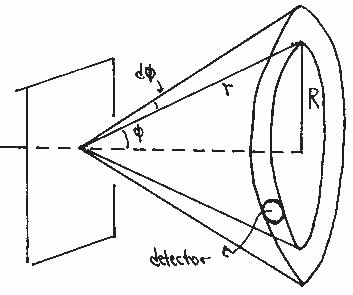
\includegraphics[width=2.375in,height=1.95833in]{images/04_rutherford/image020.jpg}
  \end{center}
  
  Therefore, by substituting for $dm$ the equation found above,
  \begin{equation*}
  y = \frac{Q \cdot dm}{2\pi r^2\sin(\phi)\,d\phi} = \frac{Q\pi ntb^2\cot(\phi/2)\csc^2(\phi/2)\,d\phi}{8\pi r^2\sin(\phi)\,d\phi}
  \end{equation*}
  Apply the trigonometric identity $\sin 2a = 2 \sin a \cos a$, where
  $\phi/2 = a$ (\emph{n.b.}: the identity is a simpler form of the identity,
  $\sin (a+b) = \sin a \cos b + \cos a \sin b$), and it follows that,
  \begin{equation*}
  y = \frac{Qntb^2\cot(\phi/2)\csc^2(\phi/2)}{16r^2\sin(\phi/2)\cos(\phi/2)} = \frac{Qntb^2\cos(\phi/2)\csc^2(\phi/2)}{16r^2\sin^2(\phi/2)\cos(\phi/2)}
  \end{equation*}
  which reduces to Rutherford's formula (5).]}
\end{equation}


Since
\begin{equation*}
b = 2NeE / mu^2 , \footnote{{[}Derived in note 13
  above.{]}}
\end{equation*}
we see from this equation that a number of $\alpha$~particles
(scintillations) per unit area of zinc sulphide screen at a given
distance $r$ from the point of incidence of the rays is
proportional to

\begin{quote}
(1) cosec\textsuperscript{4}($\phi$/2) or
1/$\phi$\textsuperscript{4} if $\phi$ be small;

(2) thickness of scattering material $t$ provided this is small

(3) magnitude of central charge $Ne$ {[}squared{]}

(4) and is inversely proportional to $(mu^2)^2$, or to the fourth
power of the velocity if $m$ be constant.
\end{quote}

In these calculations, it is assumed that the $\alpha$ particles
scattered through a large angle suffer only one large deflexion. For
this to hold, it is essential that the thickness of the scattering
material should be so small that the chance of a second encounter
involving another large deflection is very small. If, for example, the
probability of a single deflexion $\phi$ in passing through a
thickness $t$ is 1/1000, the probability of two successive
deflexions each of value $\phi$ is $1/10^6$, and is negligibly small.

The angular distribution of the $\alpha$~particles scattered from a thin
metal sheet affords one of the simplest methods of testing the general
correctness of this theory of single scattering. This has been done
recently for $\alpha$ rays by Dr. Geiger, who found that the
distribution for particles deflected between 30$^\circ$ and 150$^\circ$ from a thin
gold-foil was in substantial agreement with the theory. A more detailed
account of these and other experiments to test the validity of the
theory will be published later.\\
\centerline{* * *}
%
\subsection*{\S6.\ Comparison of Theory with Experiments}
\centerline{* * *}
Geiger{[}'s experiments{]} showed that the most probable angle of
deflection for an atom was nearly proportional to its atomic weight. It
consequently follows that the value of $N$ for different atoms
should be nearly proportional to their atomic weights, at any rate for
atomic weights between gold and aluminum.

Since the atomic weight of platinum is nearly equal to that of gold, it
follows from these considerations that the magnitude of the diffuse
deflexion of $\alpha$ particles through more than $90^\circ$ from gold and the
magnitude of the average small angle scattering of a pencil of rays in
passing through gold-foil are both explained on the hypothesis of single
scattering by supposing the atom of gold has a central charge of about
$100e$.\\[5pt]
\centerline{* * *}
%
\subsection*{\S7.\ General Considerations}

In comparing the theory outlined in this paper with the experimental
results, it has been supposed that the atom consists of a central charge
supposed concentrated at a point, and that the large single deflexions
of the $\alpha$~and $\beta$~particles are mainly due to their passage
through the strong central field. The effect of the equal and opposite
compensating charge supposed distributed uniformly throughout a sphere
has been neglected. Some evidence in support of these assumptions will
now be briefly considered. For concreteness, consider the passage of a
high speed $\alpha$ particle through an atom having a positive central
charge $Ne$, and surrounded by a compensating charge of $N$
electrons. Remembering that the mass, momentum, and kinetic energy of
the $\alpha$~particle are very large compared to the corresponding
values for an electron in rapid motion, it does not seem possible from
dynamic considerations that an $\alpha$ particle can be deflected
through a large angle by a close approach to an electron, even if the
latter be in rapid motion and constrained by strong electrical forces.
It seems reasonable to suppose that the chance of single deflexions
through a large angle due to this cause, if not zero, must be
exceedingly small compared with that due to the central charge.

It is of interest to examine how far the experimental evidence throws
light on the question of the extent of the distribution of the central
charge. Suppose, for example, the central charge to be composed of
$N$ unit charges distributed over such a volume that the large
single deflexions are mainly due to the constituent charges and not to
the external field produced by the distribution. It has been shown that
the fraction of the $\alpha$ particles scattered through a large angle
is proportional to $(NeE)^2$, where $Ne$ is the central charge
concentrated at a point and $E$ the charge on the deflected
particle. If, however, this charge is distributed in single units, the
fraction of the $\alpha$ particles scattered through a given angle is
proportional to $Ne^2$ instead of $N^2e^2$.\footnote{{[}Proportionality
  to $Ne^2$ had been derived by Thomson for his atom-model.{]}} In
this calculation, the influence of mass of the constituent particle has
been neglected, and account has only been taken of its electric field.
Since it has been shown that the value of the central point charge for
gold must be about 100, the value of the distributed charge required to
produce the same proportion of single deflexions through a large angle
should be at least 10,000. Under these conditions the mass of the
constituent particle would be small compared with that of the
$\alpha$~particle, and the difficulty arises of the production of large
single deflections at all. In addition, with such a large distributed
charge, the effect of compound scattering is relatively more important
than that of single scattering. For example, the probable small angle of
deflexion of a pencil of $\alpha$~particles passing through a thin
gold-foil would be much greater than that experimentally observed by
Geiger. The large and small angle scattering could not then be explained
by the assumption of a central charge of the same value. Considering the
evidence as a whole, it seems simplest to suppose that the atom contains
a central charge distributed through a very small volume, and that the
large single deflexions are due to the central charge as a whole, and
not to its constituents. At the same time, the experimental evidence is
not precise enough to negative the possibility that a small fraction of
the positive charge may be carried by satellites extending some distance
from the centre. Evidence on this point could be obtained by examining
whether the same central charge is required to explain the large single
deflexions of $\alpha$ and $\beta$~particles; for the $\alpha$~particle
must approach much closer to the centre of the atom than the $\beta$
particle of average speed to suffer the same large deflexion.

The general data available indicate that the value of this central
charge for different atoms is approximately proportional to their atomic
weights, at any rate for atoms heavier than aluminum. It will be of
great interest to examine experimentally whether such a simple relation
holds also for the lighter atoms. In cases where the mass of the
deflecting atom (for example, hydrogen, helium, lithium) is not very
different from that of the $\alpha$ particle, the general theory of
single scattering will require modification, for it is necessary to take
into account the movements of the atom itself\footnote{{[}Compare
  Newton, \emph{Principia}, Book I, Props. 57-60, in which corrections
  are made for the motion of the central body.{]}}...

The deductions from the theory so far considered are independent of the
sign of the central charge, and it has not so far been found possible to
obtain definite evidence to determine whether it be positive or
negative. It may be possible to settle the question of sign by
consideration of the difference of the laws of absorption of the
$\beta$ particle to be expected on the two hypotheses, for the effect
of radiation in reducing the velocity of the $\beta$ particle should be
far more marked with a positive than with a negative centre. If the
central charge be positive, it is easily seen that a positively charged
mass, if released from the centre of a heavy atom, would acquire a great
velocity in moving through the electric field. It may be possible to
account in this way for the high velocity of $\alpha$~particles without
supposing that they are initially in rapid motion within the
atom.\footnote{{[}The conjecture of a positive central charge was
  confirmed in later work, lending credence to the hypothesis that the
  alpha particles ejected by radium and other radioactive materials
  originate in the atomic \emph{nuclei} of those materials. The
  $\alpha$-particle itself could now be understood to be the
  \emph{``bare'' nucleus, without the surrounding electrons}, of a
  helium atom. This accounted both for its +2 charge and for its
  extremely small size.{]}}

Further consideration of the application of this theory to these and
other questions will be reserved for a later paper, when the main
deductions of the theory have been tested experimentally. Experiments in
this direction are already in progress by Geiger and Marsden.

\section*{Geiger and Marsden's Experiments}

The most decisive experimental work corroborating the theory Rutherford 
developed was reported by Geiger and Marsden in 1913. We
quote from the introduction to their report in \emph{Philosophical
Magazine} \textbf{25} (1913), 604--623; reprinted in \emph{The World of The
Atom}, vol.\ I, 722--733:

\begin{quote}
At the suggestion of Prof. Rutherford, we have carried out experiments
to test the main conclusions of the above theory. The following points
were investigated:---


(1) Variation with angle.

(2) Variation with thickness of scattering material.

(3) Variation with atomic weight of scattering material.

(4) Variation with velocity of incident $\alpha$ particles.

(5) The fraction of particles scattered through a definite angle.

The main difficulty of the experiments has arisen from the necessity of
using a very intense and narrow source of $\alpha$ particles owing to
the smallness of the scattering effect. All the measurements have been
carried out by observing the scintillations due to the scattered
$\alpha$~particles on a zinc-sulphide screen, and during the course of
the experiments over 100,000 scintillations have been counted. It may be
mentioned in anticipation that all the results of our investigation are
in good agreement with the theoretical deductions of Prof. Rutherford,
and afford strong evidence of the correctness of the underlying
assumption that an atom contains a strong charge at the centre, of
dimensions small compared with the diameter of the atom.
\end{quote}

\section*{Experiment: Rutherford Scattering of $\alpha$ particles}

The College has built a scattering apparatus which can provide a rough
test of the hypothesis of the concentration of positive charge in the atom. 
Our apparatus includes an alpha
particle source that is directed toward a piece of gold foil; on the far
side of the foil is placed a detector. Our object is to measure how
frequently alpha particles are deflected at high angles, from 30 to 70
degrees. In our apparatus, however, rather than moving the detector, the
alpha particle source and the foil sit on an arm that swivels, and we
jointly move the particle source and foil in order to adjust the angle
between the far surface of the foil and the detector (which remains
fixed). The College's apparatus is not as precise as Geiger and
Marsden's, primarily because our alpha particle source is weak compared
to theirs.\footnote{Theirs was ``hot enough to cook a chicken,''
  according to a knowledgeable commentator.} In addition, the beam of
alpha particles is relatively wide, about thirty degrees (in
measurements taken without the gold foil in place, the detector records
about 200 counts per second at the center of the beam, and 100 counts
per second up to six or seven degrees to each side of the center).
Nevertheless, the apparatus is sufficiently precise to test Rutherford's
statement that, at a given angle $\phi$, the number of alpha particles
detected per unit area and per unit time will be proportional to
cosec\textsuperscript{4}($\phi$ /2).

Although long angle deflections are more probable than Thomson's model
of the atom would suggest, they are still relatively rare, so that
measurements need to be taken over a long period of time. In the late
afternoon lab assistants will set the angle of the detector and reset
the counter to zero, and then read the counter the following morning.
Readings will be taken between 30 and 70 degrees at intervals of 10
degrees.

During class, one may take readings at short angles, between 0 and 30
degrees, for short periods of time (between 20 and 200 seconds, using
longer periods for longer angles). These readings cannot be used to
confirm Rutherford's mathematical prediction of the probability of
deflections, but they can be compared to readings previously taken
\emph{without the gold foil in place} in order to observe, in general
terms, the effect of the foil on the alpha particle beam.

%\includegraphics[width=5.5283in,height=3.24858in]{media/image22.png}

\chapter{The Quantum Hypothesis}

\chapterprecis{Max Planck\footnotemark}

\footnotetext{Indented sections of this chapter describing Planck's 
research are drawn from Robert Resnick, \emph{Basic Concepts in 
Relativity and Early Quantum Theory} (New York: John Wiley and Sons, 
Inc., 1972), 113--116 and 119--123.}

\makeoddhead{myheadings}{\emph{Planck}}{}{\thepage}
\makeevenhead{myheadings}{\thepage}{}{\emph{The Quantum Hypothesis}}

\renewcommand{\theequation}{\arabic{equation}}

The mathematical analysis in Einstein's paper in Chapter VI is connected
to something called ``Planck's quantum hypothesis,'' and Einstein
emphasizes the strength the connection lends to his own argument.
Planck's quantum hypothesis states that microscopic light-emitting
bodies only absorb and emit energy in indivisible units or ``quanta.''
As we shall see in his paper, Einstein adopts this hypothesis and indeed
argues for a radical extension of it. Unfortunately, the work leading up
to this hypothesis involves a great deal of probability theory which we
cannot go into here. But at least the phenomena and the ways of thinking
about them that led to the quantum hypothesis can be sketched.

\section*{A. Black Body Radiation: The Phenomena, First Attempts to
Understand Them, and Planck's \emph{Empirical} Determination of a
Formula to Fit Them.}

Being hot enough will make any solid body glow visibly. The filament in
an incandescent light bulb is not undergoing any chemical reaction: it
is glowing because it is hot. Furthermore, such a glowing body will glow
in a characteristic color and will change color, up or down the spectrum
in order, if it gets hotter or cooler.

For instance, what happens when an iron bar is heated? If its
temperature gets high enough, it starts to glow. Some of the energy
absorbed as heat is given off as light. This emitted light first becomes
visible when it is red-hot. (In fact at lower temperatures a body
``glows'' in the infra-red range, that is, at frequencies too low for
human eyes to see. This is what makes infrared photography possible.) As
the temperature rises the bar changes to other colors, up through the
spectrum, and eventually becomes blue-hot.

Why does it have distinct colors along the way? If the frequencies at
which it can emit light were all equally entitled to an equal share of
the energy, like the piano strings or the air molecules, we'd expect
that the blend of colors given off by the bar would always be the same
and that only the intensity of its glow would increase with increasing
temperature. But, instead, as we heat the bar, it goes through a phase
of intense red, a later phase of intense yellow, etc. For some reason,
at a certain range of temperatures, the bulk of the light-energy is
emitted at the red frequency, but at a higher temperature range yellow
is preferred.

Well before 1900, it was known that electromagnetic waves were absorbed
and emitted by bodies. These waves could be in the form of infrared
radiation (also known as thermal radiation or heat), visible light,
ultraviolet light, or x-rays. Anything that is at a temperature above
absolute zero will emit some kind of light in the infrared.

Nothing can emit for very long unless it is also absorbing light at some
frequency. In general, the more the body absorbs, the more it will emit.
Once a body absorbs light, assuming the body is dense enough, the energy
of the light will come to some kind of equilibrium within the body and
the emitted light will be in a range of frequencies, with a peak at some
frequency that depends on the temperature and, to some extent, on the
make-up of the body. The dependence on the make-up of the body gets less
and less as the body becomes more uniformly dense (so that equilibrium
of frequencies is achieved and conduction and convection do not carry
off some of the heat) and blacker (so that more and more light is
absorbed in order to be emitted).

\begin{quotation}
The radiation emitted by a body as a result of its temperature is called
\emph{thermal radiation}. All bodies emit such radiation to their
surroundings and absorb such radiation from it. If a body is at first
hotter than the surroundings it will cool off because its rate of
emitting energy exceeds its rate of absorbing energy. When \emph{thermal
equilibrium} is reached, the rates of emission and absorption are equal.

Matter in a condensed state (i.e., solid or liquid) emits a continuous
spectrum of radiation. The details of the spectrum depend strongly on
the temperature. At ordinary temperatures most bodies are visible to us
not by their emitted light but by the light they reflect. If no light
shines on them we cannot see them. At very high temperatures, however,
bodies are self-luminous. We can see them glow in a darkened room (hot
coals, e.g.). But even at temperatures as high as several thousand
degrees Kelvin, well over 90\% of the emitted thermal radiation is
invisible to us, being in the infrared part of the electromagnetic
spectrum. Self-luminous bodies are quite hot, therefore.

If we were to steadily raise the temperature of a hot body, we would
observe two principal effects: (1) the higher the temperature, the more
the thermal radiation emitted---at first the body appears dim, then it
glows intensely; and (2) the higher the temperature, the higher the
frequency of that part of the spectrum radiating most intensely-\/-the
predominant color of the hot body shifts from ``red heat'' to ``white
heat'' to ``blue heat.'' Since the quality of its spectrum depends on
the temperature, we can estimate the temperature of a hot body, such as
a star or a glowing chunk of steel, by analyzing the radiation it emits.
There is a continuous spectrum of radiation emitted, the eye seeing
chiefly the color corresponding to the most intense emission in the
visible region.

The detailed form of the spectrum of the thermal radiation emitted by a
hot body at a given temperature depends somewhat upon the composition of
the body. There is one class of hot bodies, however, called \emph{black
bodies}, which emit thermal radiation with the same spectrum at a given
temperature, regardless of the details of their composition. Such bodies
have surfaces that absorb all the thermal radiation incident upon them
and, because they do not reflect light, appear black. An object coated
with a diffuse layer of black pigment, such as lamp black or bismuth
black, is (nearly) a black body. A cavity in a body, open to the outside
by a small hole, is also a black body, as we shall soon explain. A
theoretical understanding of black body, or cavity, radiation was a
major goal of physicists before the turn of the {[}twentieth{]} century.

Consider first the experimental observations. The spectral distribution
of black-body radiation is described by a quantity
$\Re_T(\nu)$ called the \emph{spectral radiancy}, which
is defined so that the quantity $\Re_T(\nu)\,d\nu$ is the
{[}time{]} rate at which energy is radiated per unit area of a surface
at absolute temperature \emph{T} for frequencies in the interval
$\nu$ to $\nu\! +\! d\nu$. In Fig. 1, we show the experimentally
observed dependence
%
\begin{figure}[h]
  \begin{center}
  \captionsetup{width=.8\linewidth}
  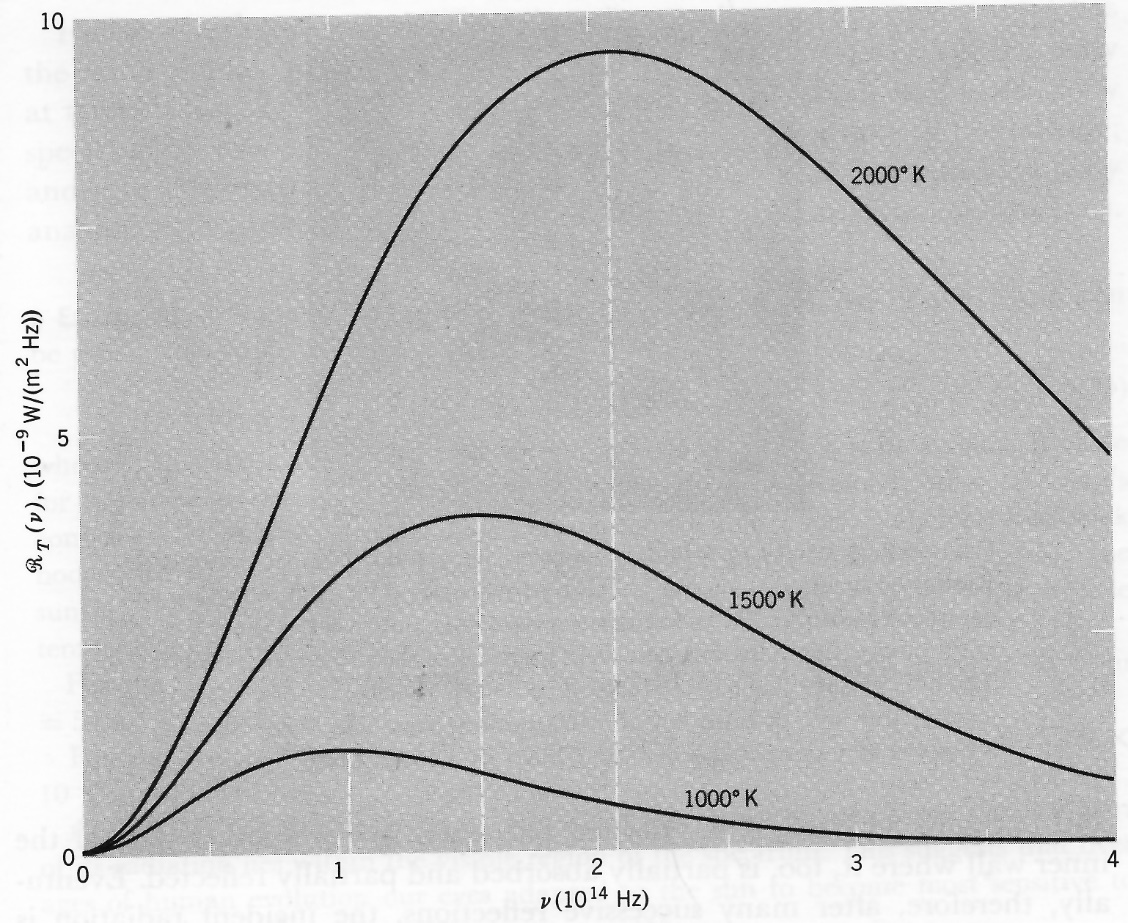
\includegraphics[width=5.125in,height=4.19792in]{images/05_planck/image001.jpg}
  \caption*{\textbf{Figure 1}. \emph{The observed spectral radiancy of a black body
  $\Re_T$, as a function of frequency $\nu$ of
  radiation, shown for black body temperatures of 1000$^\circ$, 1500$^\circ$, and 2000$^\circ$
  Kelvin. The total energy emitted per unit time per unit area (radiancy
  \emph{R\textsubscript{T}}, or area under the curve) increases rapidly
  with temperature. Note that the frequency of maximum spectral radiancy
  (dashed line) increases linearly with temperature (Wien's displacement
  law). The visible region of the spectrum is off scale to the right,
  yellow being at about 5 x 10\textsuperscript{14} Hz. Most of the
  radiation is in the infrared at these temperatures.}}
  \end{center}
\end{figure}
%
of $\Re_T(\nu)$ on $\nu$ and \emph{T}. For a given
value of the frequency $\nu$, we see that the spectral radiancy
$\Re_T(\nu)$ increases with increasing temperature
\emph{T}. If we integrate the quantity $\Re_T(\nu)$ over
all frequencies $\nu$ we obtain the total energy emitted per unit
time per unit area from a black body at temperature \emph{T}. This
quantity
%
\begin{equation}
R_T = \int_{0}^{\infty}\! \Re_T(\nu)\, d\nu
\end{equation}
%
is called the \emph{radiancy}, appropriate units for it being
watts/m$^2$. It can be interpreted as the area under a
curve in Fig. 1, from which we see that it increases rapidly as the
temperature increases. The exact dependence of radiancy on temperature
is given by \emph{Stefan's law},
%
\begin{equation}
R_T = \sigma T^{4},
\end{equation}
%
in which $\sigma = 5.67 \times 10^{-8}$ watt/(m\textsuperscript{2} $^\circ$K\textsuperscript{4}) is a universal
constant called the Stefan-Boltzman constant. We also see from Fig. 1
that as the temperature \emph{T} increases, the spectral distribution of
frequencies shifts to higher values. If the frequency $\nu$ at which
$\Re_T(\nu)$ reaches its maximum value is called
$\nu_{max}$, then as \emph{T} increases
$\nu_{max}$ is displaced toward higher frequencies. This
relation,
%
\begin{equation}\tag{3a}
\nu_{max} \propto T
\end{equation}
%
is called \emph{Wien's displacement law} {[}discovered in 1894{]}. These
experimental results are consistent with the observations we discussed
earlier, namely that the quantity of thermal radiation increases rapidly
with temperature (a hot body radiates much more heat energy at higher
temperatures) and that the principal frequency of the radiation becomes
higher with increasing temperature (the color of a hot body changes from
red to white to blue).

Most black bodies used in laboratory experiments are cavities (ovens)
having a very small opening. Let's explain why such a cavity, shown
schematically in Fig.\ 2, is a black body. Radiation outside the cavity
can enter it through the hole. It then strikes the inner wall, where it
is partially absorbed and partially reflected. The reflected part then
strikes another part of the inner wall where it, too, is partially
absorbed and partially reflected. Eventually, therefore, after many
successive reflections, the incident radiation is totally absorbed by
the wall. Because the area cut out by the hole is such a very small part
of the total area of the cavity wall, we can safely neglect the (very
small) amount of the incoming radiation that can be
%
\begin{figure}[h]
  \begin{center}
  \captionsetup{width=.75\textwidth}
  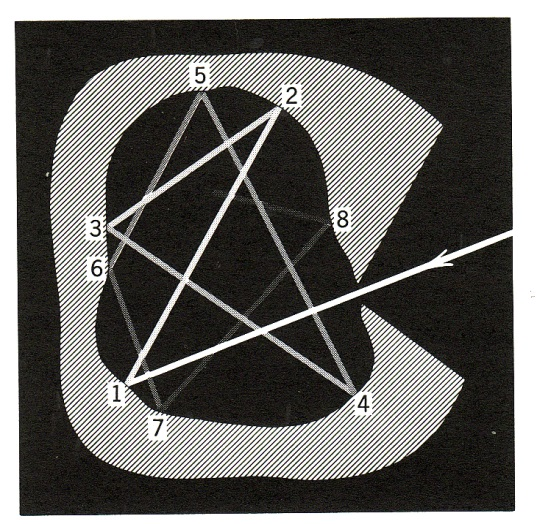
\includegraphics[width=2.4375in,height=2.38542in]{images/05_planck/image007.jpg}
  \caption*{\textbf{Figure 2}. \emph{A cavity in a body connected by a small hole to the
    outside. Radiation incident upon the hole is partly absorbed on each
    reflection and completely absorbed after many successive reflections on
    the inner surface of the cavity. (Note the diminution in intensity of
    the successive reflections.) The hole absorbs like a black body. . . .
    The hole emits like a black body.}}
  \end{center}
\end{figure}
%
reflected back out through the hole. For practical purposes we can say
that all the radiation incident on the hole from the outside is absorbed
by it. Therefore, the hole behaves just as the surface of a black body
behaves, i.e., it absorbs all the radiation incident on it. Indeed, at
low temperatures the hole appears black. If we raise the temperature by
heating the cavity walls uniformly, the hole will become self-luminous.
The inner walls emit thermal radiation into the cavity and some very
small part of this radiation will emerge from the interior through the
hole. Since the hole acts like a black surface, the spectrum of
radiation emitted by it will be characteristic of a black body.

Of course, the thermal radiation emitted by the hole is just a specimen
of the radiation filling the cavity. Therefore, the radiation inside the
cavity also has a spectrum characteristic of a black body. Since the
hole acts as a black surface, the spectrum emitted by the hole in the
cavity whose walls are at a temperature \emph{T} can be described, as
before, by the spectral radiancy $\Re_T(\nu)$. But the
spectrum of radiation \emph{inside} the cavity, called \emph{cavity
radiation}, is more conveniently described by the \emph{energy density}
$\rho_T(\nu)$, which gives the energy in the frequency
interval $\nu$ to $\nu\! +\! d\nu$ per unit volume of the cavity
at temperature \emph{T}. These quantities are proportional to one
another; that is,
%
\setcounter{equation}{3}
\begin{equation}
\rho_T(\nu) = (8\pi/c) \Re_T(\nu) \text{[equation modified]}
\end{equation}
%
. . . Suppose that we uniformly heat to a temperature \emph{T} a piece
of metal containing a cavity. The electrons in the metallic walls are
thermally agitated and emit electromagnetic radiation into the cavity.
Thermal equilibrium is established and maintained in the cavity by the
absorption and re-radiation of energy by the walls.
\end{quotation}

One attempt to understand the phenomenon of black body radiation was
that of Lord Rayleigh and Sir James Jeans. By 1905 their combined
efforts had led to the derivation of a formula for
$\rho_T(\nu)$.

\begin{quotation}
Rayleigh and Jeans showed that the radiation inside such a cavity of
volume \emph{V} consists of standing waves with nodes at the walls. They
computed the number of standing waves in the frequency interval $\nu$
to $\nu + d\nu$ to be
%
\begin{equation}
N(\nu)\, d\nu = \frac{8\pi V}{c^3}\nu^{2}\, d\nu % eqn (5)
\end{equation}
%
in which \emph{c} is the velocity of electromagnetic waves. Now, each
such standing wave contains energy. The average energy per wave, when
the system is in thermal equilibrium, can be determined from the
\textbf{classical} \emph{law of equipartition of energy}.... This states
that the average energy {[}per wave{]} is the same for each standing
wave in the cavity, independent of its frequency, i.e., the energy is
partitioned equally over all frequencies; the value of the average
energy $\bar{\varepsilon}$ depends only on the temperature \emph{T} and is given by
%
\begin{equation}
\bar{\varepsilon}(\nu, T) = \bar{\varepsilon}(T) = kT % eqn (6)
\end{equation}
%
where \emph{k} (= $1.37 \times 10^{-23}$ joule/$^\circ$K) is the
Boltzman constant. To get the average energy content per unit volume of
cavity in the frequency interval $\nu$ to $\nu\! +\! d\nu$, we
simply multiply the number of standing waves in the frequency interval
by the average energy of a wave and divide by the volume of the cavity.
In this way {[}based on the classical law of equipartition{]}, Rayleigh
and Jeans found the energy density $\rho_T(\nu) d\nu$ to be
%
\begin{equation}
\rho_T(\nu) d\nu = \frac{8\pi \nu^2}{c^3}kT\, d\nu, % eqn (7)
\end{equation}
%
which is called \emph{the Rayleigh-Jeans formula for black-body
radiation}.\footnote{Rayleigh realized in 1900 that Equation 7
  contradicted Wien's displacement law (Eq. 3a). In 1911 Paul Ehrenfest
  pointed out that it also implied what was called ``the ultra-violet
  catastrophe.''}

We compare the Rayleigh-Jeans formula, in Fig. 4, with the
experimental result for a cavity radiator at 1500$^\circ$K. As the frequency is
reduced to zero, the spectrum predicted by the Rayleigh-Jeans classical
formula does come closer and closer to the experimentally observed
spectrum. However, as the frequency is increased to large values
(ultraviolet region of the spectrum), the classical theoretical
result diverges enormously from experiment. Indeed, the classical
formula predicts an infinite energy density whereas experiment shows
that the energy density goes to zero at very high frequencies. This
completely erroneous prediction of classical physics was regarded as
such a serious shortcoming that it came to be called ``the ultraviolet
catastrophe.''

%\includegraphics[width=3.67708in,height=2.39583in]{media/image9.jpeg}
%
\begin{figure}[h]
  \begin{center}
  \captionsetup{width=3.67708in}
  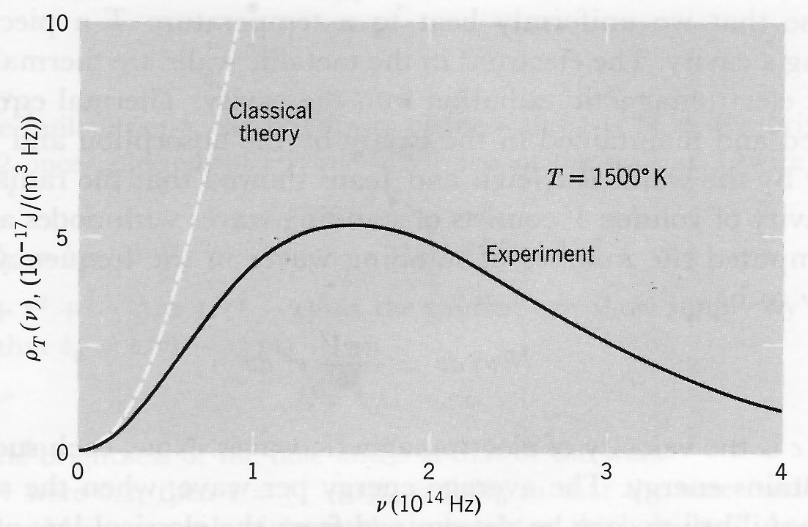
\includegraphics[width=3.67708in,height=2.39583in]{images/05_planck/image017.jpg}
  \caption*{\textbf{Figure 4}. \emph{The Rayleigh-Jeans prediction (dashed line) compared
    with the experimental result (solid line) for the energy density of a
    black body, showing the ultraviolet catastrophe.}}
  \end{center}
\end{figure}
%
\end{quotation}

In 1900 Max Planck made an independent attempt to understand black body
radiation. He began by letting $\bar{\varepsilon}(\nu, T)$ stand for the average
energy of an electromagnetic wave of frequency $\nu$ at temperature
\emph{T}, and then was able to demonstrate theoretically that when the
walls and the radiation within the cavity are in equilibrium, the energy
density, $\rho_T(\nu)$, is related to the average
energy per wave at $\nu$ and \emph{T}, $\bar{\varepsilon}(\nu, T)$, as follows:
%
\setcounter{equation}{9}
\begin{equation}
\rho_T(\nu)\, d\nu = \frac{8\pi \nu^2}{c^3}\bar{\varepsilon}(\nu, T)\, d\nu. % eqn (10)
\end{equation}
%
In an effort to arrive at an expression for $\rho_T(\nu)$
which would not predict an ultraviolet catastrophe, Planck sought to
determine a formula for $\bar{\varepsilon}$ by trying to fit the graphs of experimental
results. He arrived at the following empirical formula:
\begin{equation}
\bar{\varepsilon}(\nu) = \frac{h\nu}{e^{h\nu/kT}-1} \; , % eqn (11)
\end{equation}
where $h$ is a constant. In particular, it turned out that the
value of this constant $h$ that would give the best fit between his
formula and the experimental data was: $h = 6.63\! \times\!
10^{-34}$ joule-sec $= 4.14\! \times\! 10^{-15}$
eV-sec, which is very nearly the same as the modern value for what has
come to be known as \emph{Planck's constant.}

In Figure 5 we compare Equation 11 with Equation 6, the classical law of
equipartition:
%
\begin{equation*}\tag{6}
\bar{\varepsilon}(\nu, T) = \bar{\varepsilon}(T) = kT % eqn (6 redux)
\end{equation*}
%
%
\begin{figure}[h]
  \begin{center}
  \captionsetup{width=4.15625in}
  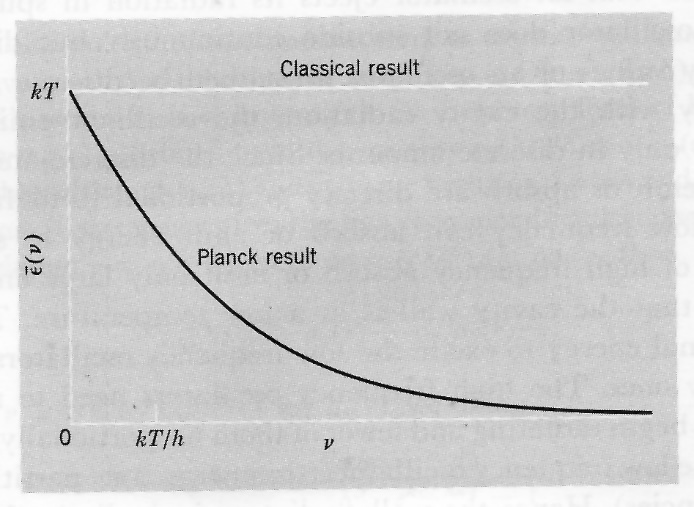
\includegraphics[width=3.15625in,height=2.30208in]{images/05_planck/image028.jpg}
  \caption*{\textbf{Figure 5}. \emph{Planck's formula for the average value of the energy,
    as a function of frequency, compared with the classical result.}}
  \end{center}
\end{figure}
%
\begin{quotation}
{[}N{]}ote that $\nu$ drops from \emph{kT} to zero in a continuous
way with increasing frequency, at first rapidly and then slowly.

When Planck used his result (Eq. 11) for $\bar{\varepsilon}$ rather than the classical value
$\bar{\varepsilon} = kT$ (Eq. 6) in the calculation of the energy density in the
cavity radiation spectrum, he found
\begin{equation}
\rho_T(\nu)\, d\nu = \frac{8\pi\nu^2}{c^3} \frac{h\nu}{e^{h\nu/kT}-1} d\nu \; . % eqn (12)
\end{equation}
This is \emph{the Planck formula for black body radiation}. Figure 6
shows a comparison of this result of Planck's {[}calculations{]} with
experiment for a temperature \emph{T} = 1595$^\circ$K. The experimental results
are in complete agreement with Planck's formula at all temperatures.

%\includegraphics[width=3.6875in,height=2.92708in]{media/image22.jpeg}
%
\begin{figure}[h]
  \begin{center}
  \captionsetup{width=4.6875in}
  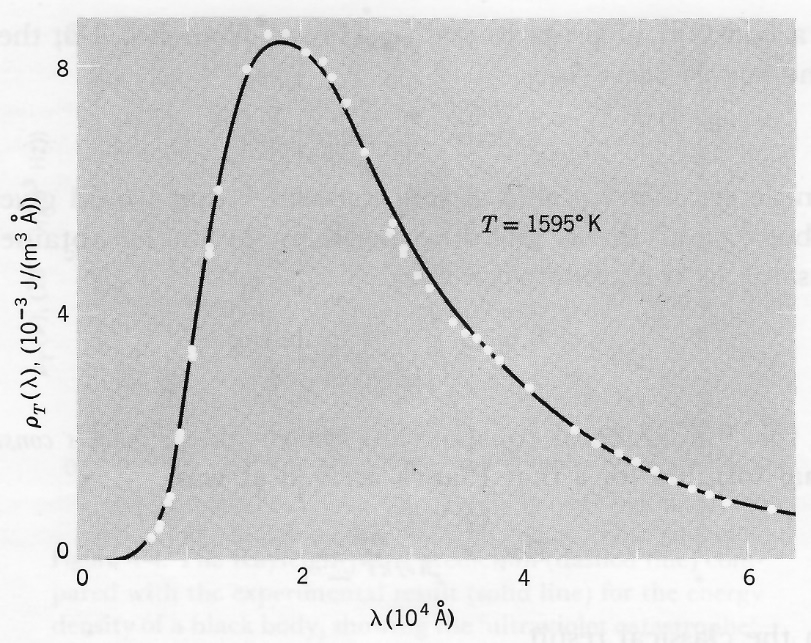
\includegraphics[width=3.6875in,height=2.92708in]{images/05_planck/image037.jpg}
  \caption*{\textbf{Figure 6}. \emph{Planck's energy density prediction (solid line)
    compared to the experimental results (circles) of the energy density of
    a black body. The data were reported by Coblentz in 1916 and apply to a
    temperature of 1595$^\circ$K. The author remarked in his paper that after
    drawing the spectral energy curves resulting from his measurements,
    ``owing to eye fatigue, it was impossible for months thereafter to give
    attention to the reduction of the data.'' The data, when finally
    reduced, led to a value of Planck's constant of 6.57 x
    10\textsuperscript{-34} J-sec.}}
  \end{center}
\end{figure}
\end{quotation}

\vspace{5pt}

\section*{B. Black Body Radiation: Planck's \emph{Theoretical}
Determination of the Formula That Fit the Experimental Results.}

Up to this point Equation 12 is merely an \emph{ad hoc} formula based on
Equation 11, which had been constructed to fit the experimental results.
Planck was convinced that it was right. Yet, theorist that he was, he
wanted more: he wanted a \emph{theoretical} derivation of Equation 11
that would explain why it was so, giving it physical meaning. We shall
ignore most of the details and, instead, focus on Planck's fundamental
modification of the classical view.

In thinking about the black-body problem, Planck had been guided by
Hertz's discovery (which may have been demonstrated in Junior
Laboratory) that oscillating charged particles---parts of tiny elastic
systems of some sort---presumably parts of atoms---emit electromagnetic
waves, which meant that cavity radiation must originate in
submicroscopic electric oscillators in the cavity walls. He reasoned
that heating a material body ought to set microscopic systems of charged
particles vibrating, for according to Maxwell they should be made to
resonate harmonically by incoming light of the proper frequencies, and
they would also be jostled by the vibratory heat motions of their
neighbors. In turn a vibrating electric charge should generate light of
the same frequency as its own vibration, again in accordance with
Maxwell's theory.

Furthermore, since the character of cavity radiation had been shown to
be independent of the material of the cavity walls, Planck had felt free
to make possibly artificial assumptions about the character of the
oscillators: He had supposed them all to be \emph{simple harmonic
oscillators}. In this analogy, Planck imagined that the cavity walls
consisted of tiny `springs' of force constants $\beta$, on the ends of
which were charged particles of masses \emph{m}. As we saw in Junior
Laboratory, this meant that each such oscillator would have a natural
frequency given by
\begin{equation}
\nu = \frac{1}{2\pi}\sqrt{\frac{\beta}{m}} \; . % eqn (13)
\end{equation}
That is, each of them had its own fixed frequency, determined by the
force binding the charge to its equilibrium position, and by the mass of
the charge.

Since the range of frequencies in cavity radiation is assumed to be
continuous, the assumption must be that the cavity walls contain large
numbers of oscillators of all frequencies represented in the radiation.
When any oscillator is vibrating at its fixed frequency, it is radiating
electromagnetic waves of the same frequency; and it is losing energy.
The temperature of the cavity walls will drop unless the lost energy is
replaced. It can be replaced by absorption of radiant energy; each
oscillator will absorb energy only of its natural frequency. But the
energy can also be replaced by heat supplied to the cavity walls: The
cavity is kept in a constant-temperature oven. The available energy will
be constantly re-distributed among the various oscillators, because of
their constant absorption and radiation of energy.

Considering the temperature \emph{T} to be fixed, Planck set out to
determine how, on the average, the total amount of energy in the cavity
at temperature \emph{T} would distribute itself on the average among the
various oscillators of different natural frequencies, $\nu$, of
vibration. That is, Planck tried to \emph{derive} the formula for
$\bar{\varepsilon}(\nu)$ (Eq. 11), which he had already arrived at by matching the
experimental results. This \emph{equilibrium distribution} of energy
among the oscillators will, in turn, determine how the energy density,
$\rho_T(\nu)$, of the cavity radiation varies with
frequency.

So, Planck had to answer the question: If, of the portions of energy
given to all the oscillators at a given moment, we consider the subset
consisting of those amounts of energy allotted to the oscillators of
natural frequency $\nu$, how do those amounts of energy distribute
themselves among the latter? Planck's first insight was that his
question was analogous to a question that had already been answered by
Ludwig Boltzmann, namely: How does the energy allotted to a set of gas
molecules in a closed container at a constant temperature \emph{T}
distribute itself among the individual molecules? These molecules have
an average kinetic energy, which is the analogue to Planck's $\bar{\varepsilon}(\nu)$.
Stated as a proportion the analogy is roughly:

\begin{quote}
(all gas molecules in the container) : (all oscillators of natural
frequency $\nu$ in the cavity walls) :: (all gas molecules in the
container having energy $\varepsilon$) : (all oscillators of natural
frequency $\nu$ having energy $\varepsilon$ in the cavity walls).
\end{quote}

Because of the large numbers of molecules and because of the fact that
they are constantly colliding, Boltzmann assumed that the energy
eventually became distributed among the molecules in a stable way. Using
probability theory as well as mechanics, Boltzmann imagined that, at any
given time, each of the $N$ molecules in a given volume of a gas would
have one of, say, $n$ different energy states. His problem was to
find the probability of the various possible distributions of particles
among these $n$ energy states. By calculating the total number of
ways in which each such distribution could be achieved, Boltzmann was
able to determine the most probable distribution of particles among the
available energy states. That is, for each of the available energy
states, $\varepsilon$, he determined the fraction,
$\Delta N_{\varepsilon}/N$, of the total number of molecules,
\emph{N,} that had energy $\varepsilon$, in the most probable distribution:
%
\begin{equation}
\frac{\Delta N_{\varepsilon}}{N} \propto e^{-{\varepsilon}/kT} % eqn (14)
\end{equation}
%
where \emph{e} is the base of natural logarithms, \emph{T} is the
absolute temperature, and \emph{k} is Boltzmann's constant, given by the
gas constant \emph{R} divided by Avogadro's number. The proportionality
(14) implies that the fraction $\Delta N_{\varepsilon}/N$
decreases as $\varepsilon$, the energy state considered, increases.

In order to find the way energy would distribute itself among his
hypothetical oscillators, Planck made use of the Boltzmann distribution
(14). He proceeded in somewhat the following way.

Consider an oscillator of mass $m$ and force constant $\beta$; let
its displacement be $x$ and its momentum $p$ =
$m(dx/dt)$. Its potential energy will be
$(1/2)\beta x^2$ and its kinetic energy $(1/2)m(dx/dt)^{2} = p^{2}/2m$.
Therefore, its total energy is\footnote{You may want to review the
  second semester junior lab manual treatment of the pendulum for what
  follows. Potential energy should equal the work done against the
  restoring force in moving the mass $m$ from zero to displacement
  $x$. The restoring force is $F = - \beta x$. Therefore the
  potential energy is this force integrated from 0 to $x$. One must
  integrate over $x$ rather than write $Fx$ because the force
  varies with $x$.}

\begin{equation}
\varepsilon = \frac{p^2}{2m} + \frac{\beta x^2}{2} % eqn (15)
\end{equation}

Its frequency, which should be regarded as fixed in what follows, is
given by Equation 13.

Equation 15 can be viewed as the equation of an ellipse in the
(\emph{p,x}) plane (this plane is called the \emph{state domain} by
Planck), where $\sqrt{2m\varepsilon}$ and $\sqrt{2\varepsilon/\beta}$ are the semi-minor and
semi-major axes\footnote{According to the Sophomore Mathematics manual,
  \emph{A Cartesian Survey of the Conic Sections}, when the equation for
  an ellipse centered at the origin is put into standard form:\\
  \(\frac{x^{2}}{a^{2}} + \frac{y^{2}}{b^{2}} - 1 = 0\), according as
  $a$ is greater or less than $b$, the major axis is of
  length $2a$, along the $x$-axis, or of length $2b$,
  along the $y$-axis.} of the inmost ellipse in Figure 7, labeled
  $\varepsilon = h\nu$. The area of the inmost ellipse will be\footnote{Given
  the equation of the ellipse in the previous note, one-fourth of the
  ellipse would correspond to $y = b[1 - (x/a)^2]^{1/2}, x \geq 0$.

  Then the area contained by the ellipse would be given by:

  \({A = \ 4\int_{0}^{a}{b(1 - \frac{x^{2}}{a^{2}}})}^{1/2}dx = \ \frac{4b}{a}\int_{0}^{a}{({a^{2} - \ x^{2})}^{\frac{1}{2}\ }}dx = \ \frac{4b}{a}\lbrack\frac{x}{2}({a^{2} - \ x^{2})}^{\frac{1}{2}\ } + \ \frac{a^{2}}{2}\sin^{- 1}({\frac{x}{a})}\rbrack_{0\ }^{a} = \ \pi ab\),

  where the indefinite integral is found from a table of integrals.}
%
\begin{equation}
A_1 = \pi p_{max}x_{max} = \pi\sqrt{2m\varepsilon}\sqrt{2\frac{\varepsilon}{\beta}} = 2\pi\varepsilon\sqrt{m/\beta} = \frac{\varepsilon}{\nu}. % eqn (16)
\end{equation}
%\includegraphics[width=4.13542in,height=2.38542in]{media/image29.png}
%
\begin{figure}[h]
  \begin{center}
  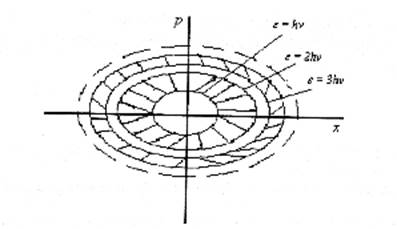
\includegraphics[width=4.13542in,height=2.38542in]{images/05_planck/image050.jpg}
  \caption*{\textbf{Figure 7}. \emph{Ellipses in the state domain.}}
  \end{center}
\end{figure}
%
Let us define a constant $h$, such that $h = A_1 = \varepsilon/\nu$. Previously Planck had showed that the area integral,
$\int\! dp\, dx$, does not vary over time. One way to think of this is to
notice that if each of the points $(p,x)$ inside the inmost ellipse
is given an additional energy of $h\nu$ (for example, by pushing a
pendulum or a spring with an additional force), then each of these
points will be displaced to the annular region between the ellipses
labeled $\varepsilon = h\nu$ and $\varepsilon = 2h\nu$, respectively (the inmost
cross-hatched annulus in the diagram). Thus, this annular region, equal
to the area of the second ellipse, $A_2$, minus that
of the first, $A_2 - A_1$,
also has area $h$, as does every annular region between two
consecutive ellipses. The entire state domain (the
${[}\emph{p,x}{]}$-plane) is thus naturally divided into non-overlapping
areas of size $h$, each of which corresponds to an amount of energy
= $h\nu$. It remains to associate a probability with each annular
region and then to take the limit of the sum of these probabilities as
the areas of the annular regions shrink to zero. But this is given to us
by the Boltzmann distribution, Equation 14.

Identifying $\varepsilon$ in Equation 14 with $h\nu$ gives us the result
that the probability of an oscillator of frequency $\nu$ having
energy $\varepsilon = h\nu$, that is, $P(\nu, h\nu)$, or, equivalently, the
fraction of the total number of oscillators of frequency $\nu$ that
have energy $\varepsilon = h\nu$, $\Delta N_\varepsilon/N$,
is
%
\begin{equation*}
P(\nu, h\nu) = Ce^{-h\nu/kT}.
\end{equation*}
%
(\emph{C} is the constant of proportionality, to be determined.)
Analogously, for any whole number \emph{n}, we obtain that the
probability of an oscillator of frequency $\nu$ having energy
$n\varepsilon = nh\nu$ is

\begin{equation}
P(\nu, nh\nu) = Ce^{-nh\nu/kT}. % eqn (17)
\end{equation}

This is the probability associated with the annular region between the
ellipses $\varepsilon = (n-1)h\nu$ and $\varepsilon = nh\nu$.

The constant \emph{C} is determined by adding up all the probabilities, 
which must equal 1;\footnote{The last step to the equation relies on an
  identity that is part of the "toolkit" of physicists and
  mathematicians, derivable using Taylor's theorem:

  \emph{(1 - x)\textsuperscript{-1} = 1 + x + x\textsuperscript{2} +
  x\textsuperscript{3} + \ldots{}}

  We let $x = e^{-h\nu/kT}$, and writing out
  some of the summation, we find that the identity is applicable.}
%
\begin{equation}
\sum_{n=0}^{\infty} P(\nu, nh\nu) = \sum_{n=0}^{\infty} Ce^{-nh\nu/kT} = C(1 - e^{-h\nu/kT})^{-1} = 1, % eqn (18)
\end{equation}
%
from which it follows that
\begin{equation}
C = 1 - e^{-h\nu/kT}. % eqn (19)
\end{equation}
If we want to find the average energy, $\bar{\varepsilon}(\nu, T)$, of \emph{all} the
oscillators having the frequency $\nu$ at temperature \emph{T}, we
multiply each of the energies, $h\nu$, $2h\nu$, $3h\nu$, \ldots
, by the probability of an oscillator's having that energy, and add up
all the terms:
%
\begin{equation}
\bar{\varepsilon}(\nu, T) \approx Ch\nu\left(e^{-h\nu/KT}+2e^{-2h\nu/kT}+\cdots\right) = Ch\nu e^{-h\nu/kT}\left(1-e^{-h\nu/kT}\right)^{-2}. % eqn (20)
\end{equation}
%
where, be it noted, we have had to include the possibility that an
oscillator have zero energy.\footnote{We have again made use of an
  identity, derivable from Taylor's Theorem,

  \emph{(1 -- x)\textsuperscript{-2} = 1 + 2x + 3x\textsuperscript{2} +
  4x\textsuperscript{3} + \ldots{} }

  And we again let $x = e^{-h\nu/kT}$ and
  factor that out, then use this identity to get the last expression in
  Equation 20.} Substituting our value for \emph{C}, (19), into Equation
20, we obtain for the average energy of the oscillators of frequency
$\nu$ at temperature \emph{T:}\footnote{The equation gets its
  right-hand form by multiplication of both numerator and denominator by
  $e^{h\nu/kT}$.}
%
\begin{equation}
\bar{\varepsilon}(\nu, T) \approx \frac{h\nu e^{-h\nu/kT}}{1-e^{-h\nu/kT}} = \frac{h\nu}{e^{h\nu/kT}-1}, % eqn (21)
\end{equation}
%
which would be identical with Equation 11 if the ``$\approx$'' were replaced
by ``=.``

We observe that, so far, Planck has been considering finite increments
in energy, of amount $h\nu$. Equation 21 is thus, according to the
notions of all earlier physics, only approximate; to obtain the exact
expression, it would normally be necessary to take the limit of Equation
21 as \emph{h} goes to zero. If this is done, however, we find
that\footnote{We let $a = h\nu/kT$, and we also recall that from
  junior math, $e^a$ is expressible in the form
\begin{equation*}
e^a = 1 + a + \frac{a^2}{2!} + \frac{a^3}{3!} + \cdots + \frac{a^n}{n!} + \cdots
\end{equation*}
  If we now write
\begin{equation*}
\bar{\varepsilon}(\nu, T) = \frac{kTa}{e^a - 1}
\end{equation*}
  and expand \emph{e\textsuperscript{a}}, the denominator will go to
  \emph{a} as \emph{h} and \emph{a} go to zero, which cancels with the
  \emph{a} in the numerator, leaving \emph{kT}.}
%
\begin{equation*}
\bar{\varepsilon}(\nu, T) \rightarrow kT\quad \text{as}\quad h \rightarrow 0.
\end{equation*}
%
Substituting this expression---$\bar{\varepsilon}(\nu, T) = kT$ {[}Eq.
6{]}---for the average energy into Equation 10, gives for the energy
density the Rayleigh-Jeans formula, Equation 7, which, as we have seen,
is in disagreement with experiment and is theoretically unacceptable in
that it implies the ``ultraviolet catastrophe.''

Now, in the classical calculation of the average energy of a large
number of things of the same kind in thermal equilibrium with each other
at temperature \emph{T} (a calculation that leads to the Equipartition
Law, Eq.\ 6), it was assumed that the energy $\varepsilon$ was a continuous
variable. However, as we have seen, Equation 21, \emph{without taking
the limit}, implies an equation for the energy density, Equation 12,
that accords with experiment (Fig.\ 6). Thus, in order to derive the
equation which fits the experimental results, Planck was forced to say
that the correct expression for $\bar{\varepsilon}(\nu, T)$ must be, not the
approximate Equation 21, or the exact equation resulting from allowing
the annular regions to shrink, but rather Equation 11. In other words,
he had to deny the assumption that the energy $\varepsilon$ varies
continuously. He could not allow \emph{h} to approach zero but, instead,
had to assume that the amount of energy assigned to an oscillator of
frequency $\nu$ must be an integral number of units $\Delta\varepsilon = h\nu$ of
energy---``energy \emph{quanta},'' as Planck called them---where
\emph{h} was the non-zero constant whose value he had determined by
fitting his Equation 11 to the empirical data. We have then, for nonzero
\emph{h}, a theoretical formula which describes the empirical results.
What does it mean? How is the meaning of \emph{h} different now as
compared with its meaning when it was first encountered above where it
was defined as $\varepsilon/\nu$?

\begin{quote}
One can understand the results of Planck's assumption physically in this
way. The electromagnetic waves in the cavity originate from radiation
given off by electrons that are thermally agitated and oscillate in the
walls of the cavity. The electronic oscillators in the cavity wall are
pictured classically as radiating their energy smoothly as their motion
gradually subsides. Planck assumed instead that an oscillator ejects its
radiation in spurts. Thus the energy of an oscillator does not subside
continuously but discretely. The allowed energy values of an oscillator
must then be discrete and, as it exchanges energy with the cavity
radiation, the oscillator emits or absorbs radiant energy only in
discrete amounts. Since the discrete energies that an oscillator can
emit or absorb [$\Delta\varepsilon = h\nu$] are directly proportional to its
frequency, the oscillators of low frequency can absorb or emit energy in
small packets whereas those of high frequency absorb or emit only large
energy packets. Now imagine that the cavity wall is at a low
temperature. Then there is sufficient thermal energy to excite the low
frequency oscillators, but not the high frequency ones. The high
frequency oscillators need to receive much more energy to begin
radiating and fewer of them proportionally are activated compared to the
low frequency oscillators (the energy is not partitioned equally over
all frequencies). Hence the walls radiate principally in the long
wavelength region and hardly at all in the ultraviolet. As the
temperature of the wall is raised there is sufficient thermal energy to
activate a larger number of high frequency oscillators and the resulting
radiation shifts its character toward higher frequencies, i.e., toward
the ultraviolet. Hence the Planck assumptions quite naturally lead to
the experimental observations discussed earlier and avoid the
ultraviolet catastrophe of the classical analysis.
\end{quote}

Physicists acknowledged the remarkable predictive power of Planck's
model. Still, the fact that it relied on the quantum hypothesis was
disturbing. It seemed extremely unlikely that actual microscopic
oscillators should only absorb and emit energy in units. Certainly
macroscopic oscillators do not seen to act this way: We can (we believe)
get a pendulum to absorb energy in any continuously varying amount, just
by nudging it right; and an oscillating pendulum seems to give up its
energy to its surroundings continuously. Quantization seemed just as
unlikely to happen in any plausible microscopic picture of the
interactions between atoms and electromagnetic waves in a continuous
medium. Thus, as long as the necessity for the quantum hypothesis was
not overcome, black-body radiation seemed to stand as a question mark to
Maxwell's theory itself.

\chapter{The Photoelectric Effect}\label{ch:einstein}
\chapterprecis{Albert Einstein}

\makeoddhead{myheadings}{\emph{Einstein}}{}{\thepage}
\makeevenhead{myheadings}{\thepage}{}{\emph{The Photoelectric Effect}}

\renewcommand{\theequation}{\arabic{equation}}

\section*{Remarks}

The \emph{photoelectric effect} was discovered by Heinrich Hertz in
1887. He found that a spark passed more readily across a narrow gap in
an electric circuit if the ends of the wires were being illuminated by
ultraviolet light---when the wires were not so illuminated, the gap
between them had to be reduced in order for the spark to pass. Shortly
afterwards Wilhelm Hallwachs found that if a freshly polished zinc plate
was insulated and connected to an electroscope, it would lose an initial
\emph{negative} charge while illuminated by ultraviolet light, but that
there was no effect if the initial charge was \emph{positive}. He
concluded that negatively charged particles were being emitted under the
action of the light.

In 1900 Philipp Lenard was able to show that the negatively charged
particles emitted from metals under the action of light were identical
with the ``corpuscles'' of Thomson's cathode rays---and therefore, as we
will now say, identical with \emph{electrons}. He also showed that when
a photosensitive metal was made the cathode in a cathode ray tube and
then illuminated, a measurable \emph{photoelectric current}, carried by
these emitted electrons, passed from cathode to anode. His measurements
disclosed that this current increased steadily with the intensity of the
light falling on the cathode.

Furthermore, by opposing this photoelectric current with an
oppositely-directed electric field, Lenard was able to determine the
potential difference at which the photoelectric current was reduced to
zero---that is, the potential difference at which even the most
energetic electrons emitted from the cathode were turned back just
before they reached the anode, called the \emph{stopping potential
difference,} $\Pi$. This potential difference was a measure of the
kinetic energy with which these electrons were ejected from the
cathode.\footnote{As an emitted electron moves toward the anode against
  the electric field, its energy increases, and the work done on it by
  the field is given by the product $\Delta$\emph{Ve}, the difference in its
  potential times the charge. Since this work is done at the expense of
  the particle's kinetic energy, the particle will be brought to rest
  when its initial kinetic energy equals this product. (Compare the
  similar situation in Rutherford, Chap.~\ref{ch:rutherford}, p.~\pageref{fn:rutherford_KE}, fn.~\ref{fn:rutherford_KE}.) If this happens
  \emph{just} before it hits the anode, then its final potential
  difference with respect to the cathode is practically identical to the
  \emph{measured} potential difference between the anode and cathode.
  Assuming that all the electrons carry the same charge \emph{e}, this
  measured $\Delta$\emph{V} is directly proportional to the initial kinetic
  energy of those emitted electrons.} In this way he discovered that
this maximum kinetic energy was \emph{not} dependent on the intensity of
the illuminating light but, instead, rose with the light
\emph{frequency}.

In two major respects the photoelectric effect contradicted classical
electromagnetic wave theory:

(1) The \emph{intensity} of any wave is defined as the energy delivered
by the wave to each unit area of a surface per second.\footnote{Thus,
  for example, if all the energy in light is converted to heat upon its
  striking a perfectly non-reflecting surface, then doubling the
  intensity of the light will deliver twice as much heat per second to
  each square centimeter of the surface.} Maxwell had argued that light
is an electromagnetic wave; and he had proven mathematically that if so
then the intensity of light must be directly proportional to the square
of the \emph{amplitude}\footnote{The \emph{amplitude} of an oscillating
  quantity is the peak value which that quantity attains in each cycle,
  without regard to sign.} of the oscillating electric field which
constitutes the electric component of the wave. But the force which an
electromagnetic wave applies to an electron in its path will be
\emph{eF}, where \emph{e} is the charge on the electron and \emph{F} is
the strength of the electric field (at the location of the electron) at
any instant. If then the amplitude of the electric field increases, the
force applied to the electron at each instant likewise increases. It
would seem, then, that a more intense light beam should impart greater
kinetic energy to the electrons in its path than a light beam of lesser
intensity would. \emph{But it does not.} Increasing the light intensity
has no discernible effect on the kinetic energy of the ejected
electrons; rather it increases the \emph{number} of electrons emitted
per second from the cathode.

(2) In Maxwell's theory, the \emph{frequency} of the incident light may
play an indirect role in determining the energy imparted to
electrons---for example, the light frequency might agree or disagree
with some resonances that characterize the forces binding individual
electrons to the solid. Nevertheless such a connection must be highly
variable, and it would seem that any relation between the electron
energy and light frequency would be correspondingly complicated.
\emph{But it is not.} The relation observed between electron energy and
light frequency showed no such complexity.

Not surprisingly, in the five years between Planck's work (1900) and the
Einstein paper (1905) physicists had tried to come up with another model
that did not depend on quantization, with results ranging from partial
success to catastrophic failure (see Niels Bohr's comments in 
Chapter \ref{ch:bohr}).
Nobody was inclined to take the quantum hypothesis seriously until
Einstein adopted it.

He did more than adopt it, however. He gave a very radical answer to the
question of \emph{why} microscopic bodies could only absorb and emit
light energy in units. Planck had proposed only that the hypothetical
electrons oscillating in the radiating body emit their energy not
continuously, as Maxwell's theory would require, but rather in discrete
bursts of light, each burst containing an amount of energy, \emph{hv},
proportional to the frequency of the individual oscillating electron and
thus of the emitted light as well. He did not assume that that energy,
once emitted, would continue to travel in a discontinuous distribution,
because it would have contradicted the electromagnetic wave theory of
light, a theory that had served remarkably well. Einstein's account in
the present paper, while it harmonizes with the experimental
observations on the photoelectric effect, does contradict the
electromagnetic theory:
\begin{quote}
According to the presently proposed assumption, the energy in a beam of
light \ldots\ consists of a finite number of energy quanta, localized at
points of space, which move without subdividing and which are absorbed
and emitted only as units.
\end{quote}

Note Einstein does not call his account a \emph{theory} but rather a
``heuristic'' point of view (from ``\emph{heurisko},'' I discover)---one
intended to serve as an aid to learning or discovery.


\section*{Concerning a Heuristic Point of View about the
Creation and Transformation of Light\footnote{{[}\emph{Annalen der
  Physik}, \textbf{17} (1905), 132--148. Translated by the Editors of
  \emph{Annalen der Physik}.{]}}\\
  {\large Albert Einstein}}

There is a profound formal difference between the theoretical
representations of gases and other ponderable bodies which physicists
have constructed and Maxwell's theory of electromagnetic processes in
so-called empty space. Whereas we may consider the state of a body as
being completely determined by the positions and velocities of, to be
sure, a very large but finite number of atoms and electrons, we must use
continuous spatial functions to specify the electromagnetic state of a
region, so that a finite number of parameters cannot be considered as
sufficient to describe completely the electromagnetic state of a region
of space. According to Maxwell's theory, in all cases of pure
electromagnetic phenomena, hence in the case of light, the energy must
be considered as a continuous spatial function; whereas the energy of a
ponderable body, according to the current concepts of physicists, can be
represented by a sum taken over the atoms and electrons. The energy of a
ponderable body cannot break up into arbitrarily many, arbitrarily small
parts; whereas the energy of a ray of light emitted by a point source of
light distributes itself continuously throughout an ever-increasing
volume of space according to Maxwell's theory (or, more generally,
according to any wave theory).

The wave theory, operating with continuous spatial functions, has proved
to be correct in representing purely optical phenomena and will probably
not be replaced by any other theory. One must, however, keep in mind
that the optical observations are concerned with temporal mean values
and not with instantaneous values; and it is possible, in spite of the
complete experimental verification of the theory of diffraction,
reflection, refraction, dispersion, and so on, that the theory of light
that operates with continuous spatial functions may lead to
contradictions with observations if we apply it to the phenomena of the
generation and transformation of light.

It appears to me, in fact, that the observations of ``black-body
radiation,'' photoluminescence, the generating of cathode rays {[}by{]}
ultraviolet radiation, and other groups of phenomena related to the
generation and transformation of light can be understood better on the
assumption that the energy in light is distributed discontinuously in
space. According to the presently proposed assumption, the energy in a
beam of light emanating from a point source is not distributed
continuously over larger and larger volumes of space but consists of a
finite number of energy quanta, localized at points of space, which move
without subdividing and which are absorbed and emitted only as units.

In what follows, I want to present the thinking and indicate the facts
that have led me along the present path in the hope that the point of
view associated with these ideas may prove useful to some researchers in
their investigations.\footnote{{[}What follows is section 8 of
  Einstein's paper, sections 1--7 and 9 being here omitted. The omitted
  sections treat, among other topics, black-body radiation and Planck's
  derivation of elementary energy quanta.{]}}\\
\centerline{* * *}
%
\subsection*{VIII. On the Production of Cathode Rays by Irradiating Solid Bodies}

The traditional view that the energy of light is distributed
continuously through the region illuminated runs into great difficulty
in trying to explain photoelectric phenomena, as was outlined in a
trail-blazing paper by Lenard.\footnote{{[}\emph{Annalen der Physik}, \textbf{8}
  (1902), 169--170. We gave a brief summary of Lenard's findings above.{]}}

According to the concept that the exciting radiation consists of energy
quanta with energy content $h\nu$,\footnote{\label{fn:einstein_h}{[}Here $\nu$ is the
  light frequency and $h$ is Planck's constant. Einstein actually
  writes here not $h$ but rather a quotient of three other
  constants, introduced in omitted sections of this paper. Since there
  he shows his own expression to be equal to Planck's we take the
  liberty of substituting $h$ throughout this section. However, it
  is worth noting that his more complicated expression contains
  \emph{Avogadro's number} in the denominator. In 1905 its size was very
  conjectural.{]}} the production of cathode rays by light can be
understood as follows: Quanta of energy penetrate into the surface layer
of the body; and their energy, at least in part, is transformed into
kinetic energy of electrons. The simplest explanation is that a quantum
transfers all its energy to a single electron; we shall assume that this
occurs. However, it ought not to be excluded that electrons take up only
part of the energy of light quanta. An interior electron with kinetic
energy will have lost some of this kinetic energy by the time it reaches
the surface. Besides this we must assume that each electron will have to
do some work (an amount characteristic of the body) when it leaves the
body.\footnote{{[}The necessity for an electron to do work specifically
  to leave the surface of a body can be compared to the phenomenon of
  surface tension in a fluid. The work required is called the ``work
  function''; Einstein denotes it by \emph{P} in the expression that
  follows.{]}} The electrons lying right at the surface of the body will
leave the body with the greatest velocity normal {[}i.e.\
perpendicular{]} to the surface. The kinetic energy of such electrons is

\begin{equation*}
h\nu - P.
\end{equation*}
%
If the body is charged to the positive potential $\Pi$\footnote{{[}Thus
  there is a potential \emph{difference} $\Pi$ between the body and
  the surrounding grounded conductors, which opposes the current. This
  is exactly equivalent to what Lenard did.{]}} [\,\ldots] and if $\Pi$
is {[}just{]}\footnote{{[}We here correct an omission in the
  translation.{]}} large enough to prevent a discharge of the body, then
we must have\footnote{{[}That is, $\Pi e$,
  potential difference times charge, must equal the initial kinetic
  energy of the most energetic emitted electrons which are just stopped
  by this $\Pi$ .{]}}
%
\begin{equation*}
\Pi e = h\nu - P,
\end{equation*}
%
where \emph{e} is the electric charge of the electron, or
%
\begin{equation*}
\Pi E = Nh\nu - P'
\end{equation*}
%
where $E \: \text{[}\!= Ne\text{]}$ is the charge of a gram equivalent of a
single charged ion {[}i.e., one \emph{faraday}{]} and $P'$ is the
potential of this amount of negative charge relative to the
body.\footnote{{[}The equation $\Pi e = Nh\nu - P'$ is the
  previous equation multiplied through by Avogadro's number $N$.
  Einstein does this because in 1905 physicists had much better
  measurements for the faraday $E$ than for $e$ and Einstein
  was more confident about the size of $Nh$ than about either
  $N$ or $h$ separately. He is not worried about $P'$
  since he is about to set it to zero. {]}}

If we place $E = 9.6\times 10^3$, then $\Pi\times 10^{-8}$ is the potential
in volts that the body acquires on being irradiated in a
vacuum.\footnote{{[}The \emph{faraday} equals 96,500 cou or about 9650
  abcou. With $E$ expressed in abcoulombs and $h$ in
  erg-seconds, $\Pi$ will be given in erg/abcou or \emph{abvolts}.
  Hence $\Pi\times 10^{-8}$ will express the potential in volts. See
  Appendix.{]}}

In order to see at first if the derived relationship is of the right
order of magnitude as obtained empirically we place $P' = 0$,
$\nu = 1.03\times 10^{15}$ (corresponding to the ultraviolet limit of the
solar spectrum\footnote{{[}Sunlight comprises wavelengths as small as
  $2902\times 10^{-8}$ cm, corresponding to frequencies as great as $1.03\times 10^{15}$
  cycles/sec.{]}}) and {[}$Nh = 4.01\times 10^{-3}${]}.\footnote{{[}Einstein
  actually expresses \emph{Nh} here in terms of two other constants. His
  expression does \emph{not} contain Avogadro's number, since
  multiplying through by \emph{N} removed it from the denominator of the
  three-constant expression for $h$ mentioned in fn.\ \ref{fn:einstein_h}. 
  Note that in the cgs system of 
  measurement, Planck’s constant, $h$, has the value $6.6\times 10^{-27}\ \text{erg-sec}$.{]}} We
obtain {[}$\Pi = 4.3\times 10^8$ abvolts, so that $\Pi\times 10^{-8} =
4.3${]} volts, which agrees in order of magnitude with the results of
Lenard.\footnote{{[}In the experiments mentioned above, Lenard
  had found that when the cathode is illuminated by direct sunlight,
  electrons are emitted until the cathode acquires a potential on the
  order of a few volts.{]}}

If the derived formula is correct, then {[}$\Pi${]} must be a linear
function of the frequency whose slope {[}is independent of{]} the nature
of the material being studied.\footnote{{[}That is, the energy acquired
  by the electrons will be proportional to the frequency of the exciting
  light.{]}}

Our point of view, as far as I can see, does not contradict Lenard's
observed properties of the photoelectric phenomena. If each quantum of
energy of the exciting light gives up its energy to an electron
independently of all the other quanta, then the velocity distribution of
the electrons, that is, the characteristic of the produced cathode ray,
is independent of the intensity of the exciting radiation; on the other
hand the number of electrons leaving the body, all other conditions
being the same, will depend on the intensity of the exciting 
radiation.\\
\centerline{* * *}

\section*{Experiment: The Photoelectric Effect}

\subsection{Current is directly proportional to illumination intensity.}

If light consists of a stream of discrete quanta of energy, and if each
quantum gives up all its energy to a single electron, then the number of
electrons released per second from an illuminated photocell cathode
should equal the number of energy quanta absorbed per second by the
cathode. But the number of electrons released per second is proportional
to the \emph{cathode current}, since each electron carries a determinate
charge. And the number of energy quanta absorbed per second is
proportional to the \emph{illumination intensity}; since the very
definition of that quantity is the amount of energy absorbed, per unit
time, by unit area of the illuminated surface. Thus the current produced
by the photocell should be proportional to the illumination supplied, as
Einstein states.

To investigate this effect, a photocell is connected directly to a
sensitive picoammeter as indicated in the sketch below; set the meter to
the 2 microampere ($\mu\text{A}$) range. An ordinary
illuminating lamp makes a satisfactory light source. For a rough test of
the relation between light intensity and current, observe how the
photocurrent rises and falls when the light source is moved toward and
away from the cell.

\begin{figure}[h]
  \begin{center}
  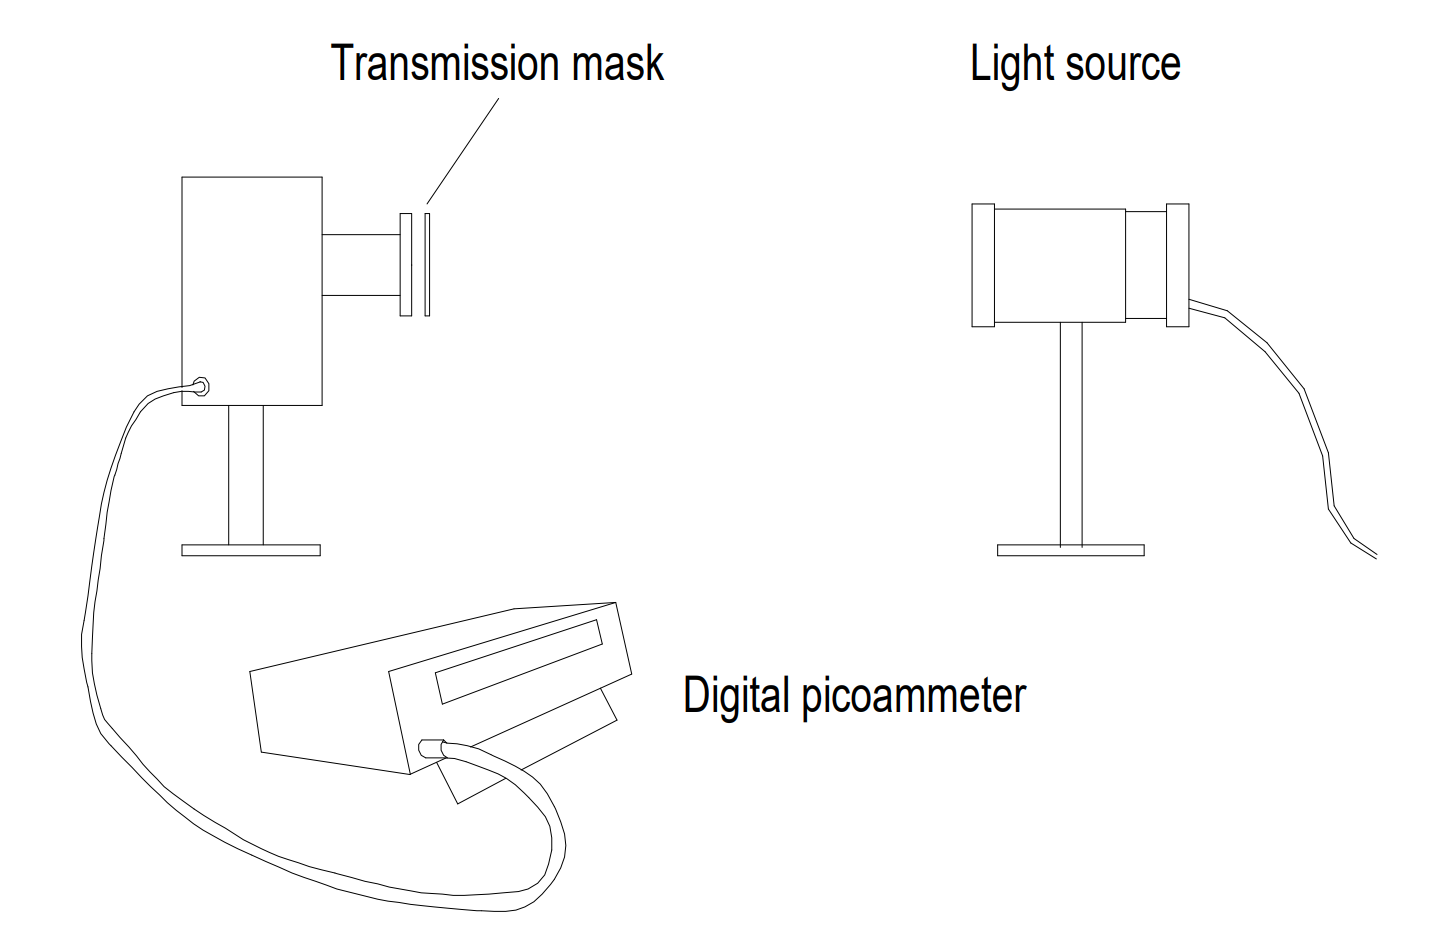
\includegraphics[width=4.08333in,height=2.77083in]{images/06_einstein/001.png}
  \end{center}
\end{figure}

Examine the \emph{variable transmission mask}. This is a strip of
transparent material on which computer-generated patterns of dots and
lines have been printed so as to block selected percentages of the
transparent area and thereby vary the intensity of the transmitted
light. The five sections transmit, respectively, 100\%, 80\%, 60\%,
40\%, and 20\% of the incident light. With the lamp aimed to illuminate
the photocell aperture, hold the transmission mask so that light passes
through the section labeled ``100\%,'' and record the current generated.
Repeat the measurement for the remaining sections and compare the
currents to the corresponding transmission percentages.

\subsection{Electron energy is directly proportional to light frequency.}

It follows from Einstein's equation $\Pi e = h\nu - P$
above that the most energetic electrons among those released from the
illuminated cathode will have kinetic energy \emph{per unit charge} of
amount
\begin{equation*}
\Pi = h\nu/e - P/e
\end{equation*}
where $\nu$~is the frequency of the incident light, \emph{e} is the
charge on the electron, and \emph{P} is a constant characteristic of the
material of the cathode. If \emph{e} is given in abcoulombs and $h$
in erg-seconds, then $\Pi$ will express this energy per unit charge
(the potential) in abvolts. As Einstein states, a
graph of $\Pi$ vs.\ $\nu$ should yield a straight line;
furthermore, it should have a slope equal to \emph{h/e}, having a value
of $4.14\times 10^{-7}$ abvolt/Hz or $4.14\times 10^{-15}$ volt/Hz.\footnote{The
  quotient of presently accepted values $h = 6.625\times 10^{-27}$ erg/Hz
  and $e = 1.6\times 10^{-20}$ abcou is $4.14\times 10^{‑7}$ abvolt/Hz.}

When illuminated, the photocell cathode will lose electrons and thus
acquire a positive potential which continues to increase so long as
electrons continue to flow from it. But, when the cathode potential
rises to a value $\Pi$~that equals the energy per unit charge of the
most energetic electron, no additional electrons will be able to reach
the anode, the photoelectric current will drop to zero, and the
potential will stop rising. An incident light beam will therefore charge
the cathode to the potential $\Pi$; and we can
investigate $\Pi$ as a function of $\nu$ by causing light of
various frequencies to charge the cathode to the corresponding
potentials.

For a source of illumination, we shall use a spectrometer diffraction
grating to separate out individual \emph{spectral lines}\footnote{Glowing
  \emph{gases}, unlike glowing solid bodies, give off light in pure,
  isolated, sharply-demarcated colors, which gives a pattern of isolated
  monochromatic lines separated by wide dark areas when passed through a
  diffraction grating. \emph{Why} this should be is a question which
  Neils Bohr addresses in our next reading: it proves to have a profound
  bearing on atomic structure.} from an intense mercury vapor lamp. The
principal lines are given in the following table:


\begin{minipage}{0.95\textwidth}
\centering
\begin{tabular}{ l l l }
 & $\lambda$ & $\nu$\\
Yellow\footnote{There are really two yellow lines in the mercury
  spectrum, at 5770 and 5882 Å, respectively; but these are not
  separable by the grating and so the line of higher frequency will
  predominate, according to Einstein's treatment.}
  & $5780$ {\small Å}\footnote{One Angstrom (Å) equals $10^{-8}$ cm.}
  & $5.19\times 10^{14}$ Hz\\

Green & $5461$ & $5.49$\\

Blue & $4358$ & $6.88$\\

Violet & $4047$ &$7.41$\\

Ultraviolet & $3655$ & $8.20$\\

\end{tabular}
\end{minipage}

\medskip

Our light source is rich in ultraviolet content and is capable of
damaging the eyes. Suitable protective shielding is provided and you
should not remove it or attempt to defeat its purpose. Needless to say,
\emph{you should avoid looking directly at the beam of light or any
reflections}. Note that the mercury vapor lamp requires a warm-up period
of about five minutes before measurements are made. Also, frequent
on-off operation will reduce the lamp life; once turned on, it is best
to leave it burning until all work for that session is completed.

The apparatus for this part of the experiment is diagrammed here.
\begin{figure}[h]
  \begin{center}
  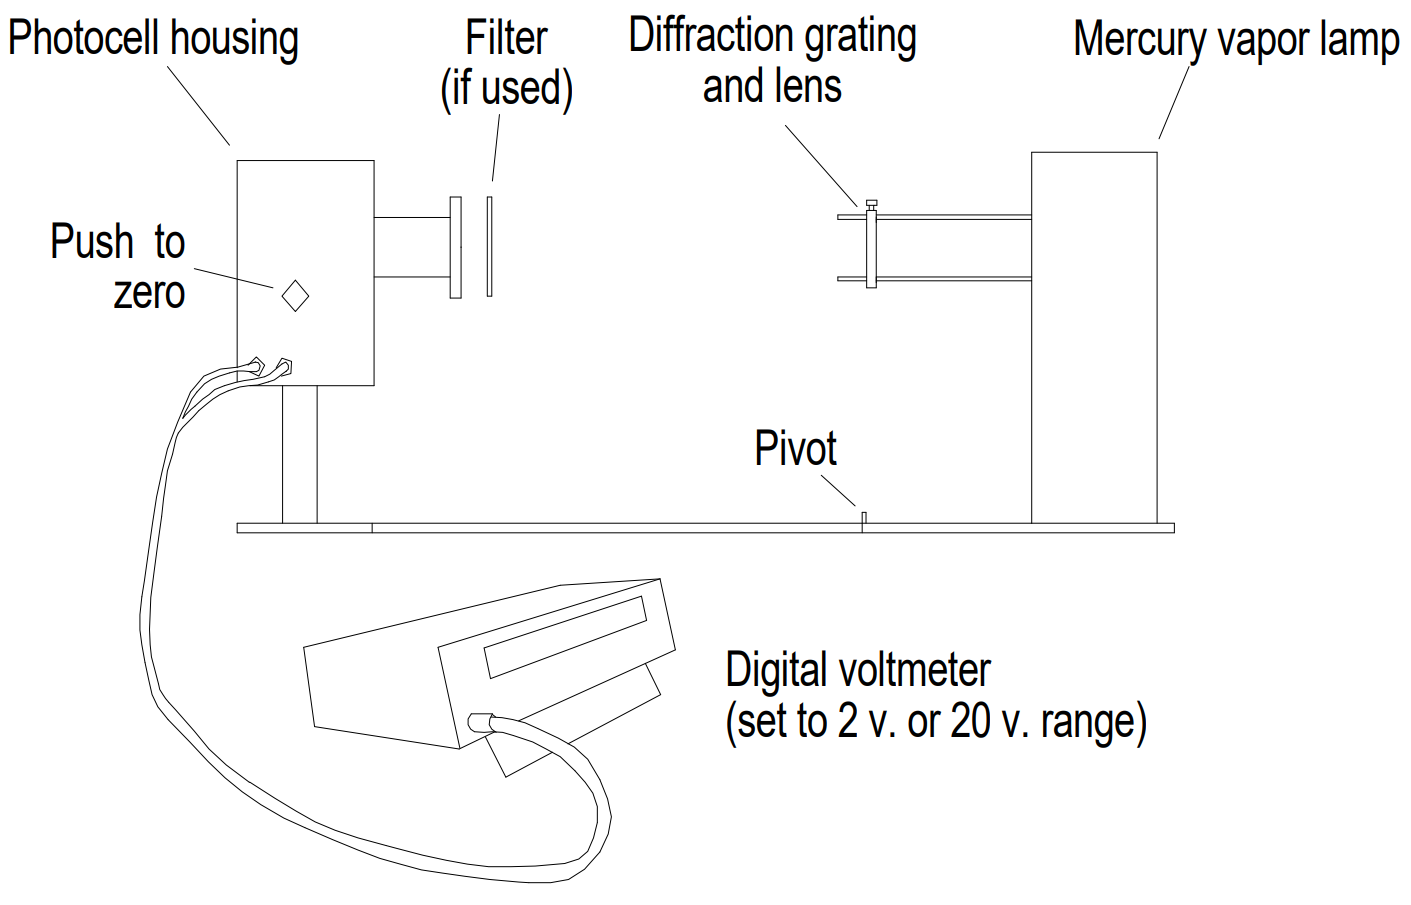
\includegraphics[width=4.08333in,height=2.77083in]{images/06_einstein/003.png}
  \end{center}
\end{figure}


Light exits through a narrow slit at the front of the lamp and is focused on
the photocell aperture by means of an adjustable lens.\footnote{The
  laboratory assistants will have already performed an internal
  alignment to insure that light falling on the aperture fully enters
  the photocell. If you wish to check this adjustment, the procedure is
  described in the final section of this chapter.} A diffraction grating is mounted adjacent to
the lens and forms a spectrum of lines on either side of the beam axis.
The spectrum is significantly brighter on one side than on the other;
make your measurements on the brighter spectrum.

The sketch below shows a top view of the apparatus. Each line of the
Mercury spectrum can be separately introduced to the photocell by moving
the cell to the appropriate position. The spectral lines will be clearly
reflected on the white mask surrounding the photocell aperture. This
mask has been made slightly fluorescent in order to reveal the location
of the otherwise invisible ultraviolet band; it will emit a blue glow
where it is illuminated by ultraviolet light.

\begin{figure}[h]
  \begin{center}
  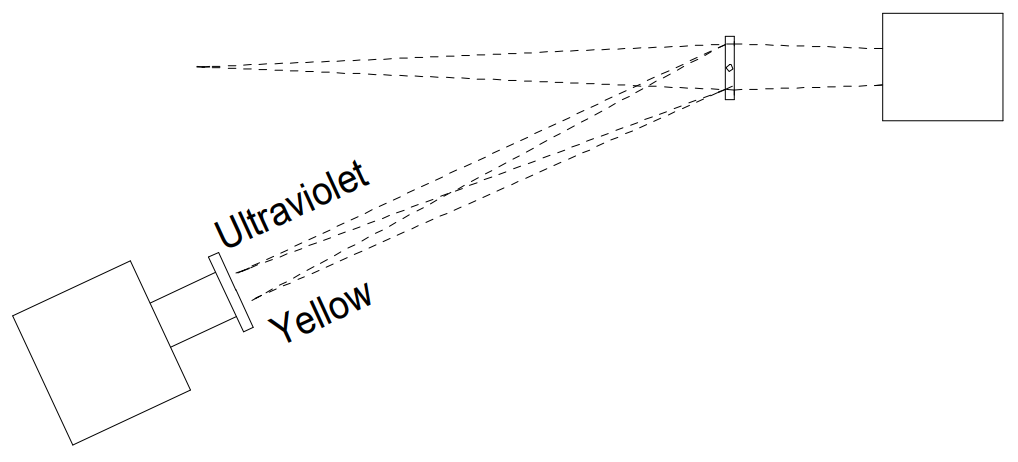
\includegraphics[width=2.91667in,height=1.33333in]{images/06_einstein/005.png}
  \end{center}
\end{figure}


A voltmeter measures the potential difference between the photocell
cathode and anode. But ordinary measuring instruments cannot be
connected to the photocell directly, since they lack sufficient
sensitivity and would actually discharge the photocell in the very
process of measuring its potential. For this part of the experiment,
therefore, the photocell unit is equipped with a battery-powered
amplifier circuit that in effect \emph{reproduces} the cell's potential
difference at a pair of auxiliary terminals. The voltmeter connected to
these terminals will indicate a potential difference equal to that
developed between cathode and anode. Turn the battery switch on at the
beginning of each session, and please remember to turn it off again when
you conclude your work.\footnote{The battery voltage can be tested at
  the two terminals marked ``test.'' Six volts is the minimum acceptable
  reading between each test terminal and the chassis.}

For each measurement, swing the photocell unit until the desired
spectral line falls on the aperture in the cell housing. Take care to
permit only one line at a time to illuminate the aperture. Also, it is
best to confine your measurements to the \emph{first order} of lines
produced by the diffraction grating. Even though the grating will
furnish two or even three orders of spectral lines, the second- and
third-order patterns overlap one another, making some lines unusable.

When measuring the green or yellow spectral lines, be sure to mount the
corresponding green or yellow filter over the face of the cell aperture.
Otherwise ambient light in the room, or even stray reflections from
other spectral lines, might enter the cell housing and cause erroneous
readings. The filters attach easily with magnetic strips. Please treat
the filters with care, as they are easily scratched.

Notice the switch labeled ``push to zero'' on the rear of the photocell
unit. You should operate this switch prior to each reading in order to
discharge any previously accumulated potential difference.

When the photocell is illuminated, and the ``zero'' switch pressed and
released, the voltmeter will gradually rise to a stable value which
represents the maximum potential $\Pi$, corresponding to the
frequency $\nu$ of the light presently being admitted to the
cell.\footnote{In some devices, the voltmeter will temporarily read
  \emph{high} and gradually \emph{decrease} to a stable value. This
  reflects a variation in the manufacturer's amplifier circuit; but the
  stable reading nevertheless indicates the actual potential difference
  in the photocell.}

Our digital voltmeters perform poorly when their batteries run down;
\emph{please} turn off the voltmeters at the end of each session. If the
readings obtained for bright spectral lines appear to be erratic, try
another voltmeter, or replace the battery. But note that when the
photocell is \emph{not} illuminated, it is normal for the voltmeter
readings to drift randomly.

\subsubsection*{INTERNAL ALIGNMENT --- Adjust only if necessary}

\begin{tight_enumerate}
\item Swing the photocell to the side having the brighter diffraction
pattern until the green line, say, falls on the white mask surrounding
the photocell aperture.

\item Roll the cylindrical light shield out of the way to reveal a second
white mask with a smaller aperture. Loosen the thumbscrew on the
photocell housing support rod and rotate the photocell unit until the
green line is centered both on the aperture of the external mask
\emph{and} the aperture of the internal mask, simultaneously. Tighten
the support rod thumbscrew securely.

\item Loosen the thumbscrew on the diffraction grating/lens assembly and
slide it back and forth on the support rods to focus the light onto the
internal white mask. Roll the cylindrical light shield back into
position; tighten the grating/lens thumbscrew to hold the assembly in
place.

\item For additional alignment accuracy, repeat steps 2 and 3 again.
\end{tight_enumerate}
	
\chapter{On the Spectrum of Hydrogen}\label{ch:bohr}
\chapterprecis{Niels Bohr}

\makeoddhead{myheadings}{\emph{Bohr}}{}{\thepage}
\makeevenhead{myheadings}{\thepage}{}{\emph{On the Spectrum of Hydrogen}}

\renewcommand{\theequation}{\arabic{equation}}

\section*{On the Spectrum of Hydrogen\footnote{{[}Address delivered before the
  Physical Society in Copenhagen, Dec. 20, 1913. Essay I from \emph{The
  Theory of Spectra and Atomic Constitution}, Cambridge, 1922.{]}}}

\emph{Empirical Spectral Laws}. Hydrogen possesses not only the smallest
atomic weight of all the elements, but it also occupies a peculiar
position both with regard to its physical and its chemical properties.
One of the points where this becomes particularly apparent is the
hydrogen line spectrum.

The spectrum of hydrogen observed in an ordinary Geissler tube consists
of a series of lines,\footnote{{[}You saw similar sharp lines in the
  last practicum.{]}} the strongest of which lies at the red end of the
spectrum, while the others extend out into the ultra violet, the
distance between the various lines, as well as their intensities,
constantly decreasing. In the ultra violet the series converges to a
limit.

Balmer, as we know, discovered (1885) that it was possible to represent
the wave lengths of these lines very accurately by the simple law
%
\begin{equation}\label{eq:bohr_1}
\frac{1}{\lambda_n} = R\left(\frac{1}{4} - \frac{1}{n^2}\right),
\end{equation}
%
where $R$ is a constant and $n$ is a whole number. The wave
lengths of the five strongest hydrogen lines, corresponding to $n
= 3, 4, 5, 6, 7$, measured in air at ordinary pressure and temperature,
and the values of these wave lengths multiplied by
%
\begin{equation*}
\left(\frac{1}{4} - \frac{1}{n^2}\right)
\end{equation*}
%
are given in the following table:\footnote{{[}Recall that an Ångstrom
  unit equals $10^{-8}$ cm. Thus, for example, 6563.04 in the second column
  actually equals $6.563 \times\  10^{-5}\ \text{cm}$. The third column,
  by Eq.\ \eqref{eq:bohr_1}, gives $1/R \times 10^{10}$.{]}}

\begin{center}
\begin{tabular}{c @{\hspace{4em}}c@{\hspace{4em}} c}
$n$ & $\lambda \cdot 10^8 \text{[Å]}$ & $\lambda \cdot \left(\frac{1}{4} - \frac{1}{n^2}\right)\cdot 10^{10}$\\
 & & \\
3 & 6563.04 & 91153.3\\

4 & 4861.49 & 91152.9\\

5 & 4340.66 & 91153.9\\

6 & 4101.85 & 91152.2\\

7 & 3970.25 & 91153.7\\
\end{tabular}
\end{center}

The table shows that the product is nearly constant, while the
deviations are not greater than might be ascribed to experimental
errors.

As you already know, Balmer's discovery of the law relating to the
hydrogen spectrum led to the discovery of laws applying to the spectra
of other elements. The most important work in this connection was done
by Rydberg (1890) and Ritz (1908). Rydberg pointed out that the spectra
of many elements contain series of lines whose wave lengths are given
approximately by the formula
\begin{equation*}
\frac{1}{\lambda_n} = A - \frac{R}{(n + \alpha)^2}
\end{equation*}
where $A$ and $\alpha$ are constants having different values for
the various series, while \emph{R} is a universal constant equal to the
constant in the spectrum of hydrogen. If the wave lengths are measured
in vacuo Rydberg calculated the value of R to be 109675.\footnote{{[}One
  over this $\times 10^{10}$ is 91178.5 (this is for a vacuum,
  not air as in the previous table).{]}} In the spectra of many
elements, as opposed to the simple spectrum of hydrogen, there are
several series of lines whose wave lengths are to a close approximation
given by Rydberg's formula if different values are assigned to the
constants $A$ and $\alpha$. Rydberg showed, however, in his
earliest work, that certain relations existed between the constants in
the various series of the spectrum of one and the same element. These
relations were later very successfully generalized by Ritz through
establishment of the ``combination principle.'' According to this
principle, the wave lengths of the various lines in the spectrum of an
element may be expressed by the formula
%
\begin{equation}
\frac{1}{\lambda} = F_r(n_1) - F_s(n_2) .
\end{equation}
%
In this formula $n_1$ and $n_2$ are whole numbers, and
$F_1(n), F_2(n), \ldots{}$ is a series of
functions of $n$, which may be written approximately
%
\begin{equation*}
F_r(n) = \frac{R}{(n +\alpha_r)^2}
\end{equation*}
%
where \emph{R} is Rydberg's universal constant and $\alpha_r$ is a
constant which is different for the different functions. A particular
spectral line will, according to this principle, correspond to each
combination of $n_1$ and $n_2$, as well as to the functions
$F_1, F_2, \ldots{}$. The establishment of this principle led
therefore to the prediction of a great number of lines which were not
included in the spectral formulae previously considered, and in a large
number of cases the calculations were found to be in close agreement
with the experimental observations. In the case of hydrogen Ritz assumed
that formula (1) was a special case\footnote{{[}``special case'':
  Formula (1) is that special case of equation (3) in which $n_1^2$
  has the value 4. Equation (3) is in turn that special case of equation
  (2) in which $F_r(n)$ and $F_s(n)$ each have
  the form $R/n^2$.]} of the general formula
%
\begin{equation}
\frac{1}{\lambda} = R\left(\frac{1}{n_1^2} - \frac{1}{n_2^2}\right) ,
\end{equation}
%
and therefore predicted among other things a series of lines in the
infra red given by the formula
%
\begin{equation*}
\frac{1}{\lambda} = R\left(\frac{1}{9} - \frac{1}{n_2^2}\right) ,
\end{equation*}
%
In 1909 Paschen succeeded in observing the first two lines of this
series corresponding to $n$ = 4 and $n$ = 5.\\
\centerline{* * *}
%
The discovery of these beautiful and simple laws concerning the line
spectra of the elements has naturally resulted in many attempts at a
theoretical explanation. Such attempts are very alluring because the
simplicity of the spectral laws and the exceptional accuracy with which
they apply appear to promise that the correct explanation will be very
simple and will give valuable information about the properties of
matter. I should like to consider some of these theories somewhat more
closely, several of which are extremely interesting and have been
developed with the greatest keenness and ingenuity, but unfortunately
space does not permit me to do so here. I shall have to limit myself to
the statement that not one of the theories so far proposed appears to
offer a satisfactory or even a plausible way of explaining the laws of
the line spectra. Considering our deficient knowledge of the laws which
determine the processes inside atoms it is scarcely possible to give an
explanation of the kind attempted in these theories. The inadequacy of
our ordinary theoretical conceptions has become especially apparent from
the important results which have been obtained in recent years from the
theoretical and experimental study of the laws of temperature
radiation.\footnote{{[}By ``temperature radiation'' Bohr refers to what
  was called ``black-body radiation'' by Planck and Einstein. In the
  following section of this paper Bohr offers his own account.{]}} You
will therefore understand that I shall not attempt to propose an
explanation of the spectral laws; on the contrary I shall try to
indicate a way in which it appears possible to bring the spectral laws
into close connection with other properties of the elements, which
appear to be equally inexplicable on the basis of the present state of
the science. In these considerations I shall employ the results obtained
from the study of temperature radiation as well as the view of atomic
structure which has been reached by the study of the radioactive
elements.

\emph{Laws of temperature radiation}. I shall commence by mentioning the
conclusions which have been drawn from experimental and theoretical work
on temperature radiation.

Let us consider an enclosure surrounded by bodies which are in
temperature equilibrium. In this space there will be a certain amount of
energy contained in the rays emitted by the surrounding substances and
crossing each other in every direction. By making the assumption that
the temperature equilibrium will not be disturbed by the mutual
radiation of the various bodies Kirchoff (1860) showed that the amount
of energy per unit volume as well as the distribution of this energy
among the various wave lengths is independent of the form and size of
the space and of the nature of the surrounding bodies and depends only
on the temperature. Kirchoff's result has been confirmed by experiment,
and the amount of energy and its distribution among the various wave
lengths and the manner in which it depends on the temperature are now
fairly well known from a great amount of experimental work; or, as it is
usually expressed, we have a fairly accurate experimental knowledge of
the ``laws of temperature radiation.''

Kirchoff's considerations were only capable of predicting the existence
of a law of temperature radiation, and many physicists have subsequently
attempted to find a more thorough explanation of the experimental
results. You will perceive that the electromagnetic theory of light
together with the electron theory suggests a method of solving this
problem. According to the electron theory of matter\footnote{{[}``One
  has been led to the conception of \emph{electrons}, i.e.\ extremely
  small particles, charged with electricity, which are present in
  immense numbers in all ponderable bodies, and by whose distribution
  and motions we endeavor to explain all electric and optical pheno-mena
  that are not confined to free ether'' (H.\ A.\ Lorentz, \emph{The Theory
  of Electrons}, 1905).{]}} a body consists of a system of electrons. By
making certain definite assumptions concerning the forces acting on the
electrons it is possible to calculate their motion and consequently the
energy radiated from the body per second in the form of electromagnetic
oscillations of various wave lengths. In a similar manner the absorption of 
rays of a given wave length by a substance can be determined by calculating 
the effect of electromagnetic oscillations upon the motion of the 
electrons[\ldots]. As is well known this has been done by Lorentz (1903). 
He calculated the emissive as well as the absorptive power of a metal for 
long wave lengths[\ldots]. Lorentz really obtained an expression for the law 
of temperature radiation which for long wave lengths agrees remarkably well
with experimental facts. In spite of this beautiful and promising
result, it has nevertheless become apparent that the electromagnetic
theory is incapable of explaining the law of temperature radiation. For,
it is possible to show, that, if the investigation is not confined to
oscillations of long wave lengths, as in Lorentz's work, but is also
extended to oscillations corresponding to small wave lengths, results
are obtained which are contrary to experiment. This is especially evident 
from Jeans’ investigations (1905) in which he employed a very interesting 
statistical method first proposed by Lord Rayleigh.

We are therefore compelled to assume, that the classical electrodynamics
does not agree with reality, or expressed more carefully, that it cannot
be employed in calculating the absorption and emission of radiation by
atoms. Fortunately the law of temperature radiation has also
successfully indicated the direction in which the necessary changes are
to be sought. Even before the appearance of the papers by Lorentz and
Jeans, Planck (1900) had derived theoretically a formula for the black
body radiation which was in good agreement with the results of
experiment. Planck did not limit himself exclusively to the classical
electrodynamics, but introduced the further assumption that a system of
oscillating electrical particles (elementary resonators) will neither
radiate nor absorb energy continuously, as required by the ordinary
electrodynamics, but on the contrary will radiate and absorb
discontinuously. The energy contained within the system at any moment 
is always equal to a whole multiple of the so-called quantum of energy 
the magnitude of which is equal to
$h\nu$, where $h$ is Planck's constant and $\nu$ is the
frequency of oscillation of the system per second. In formal respects 
Planck's theory leaves much to be desired; in certain calculations the ordinary
electrodynamics is used, while in others assumptions distinctly at
variance with it are introduced without any attempt being made to show
that it is possible to give a consistent explanation of the procedure
used. Planck's theory would hardly have acquired general recognition
merely on the ground of its agreement with experiments on black body
radiation, but, as you know, the theory has also contributed quite
remarkably to the elucidation of many different physical phenomena, such
as specific heats, photoelectric effect, X-rays and the absorption of
heat rays by gases. These explanations involve more than the qualitative
assumption of a discontinuous transformation of energy, for with the aid
of Planck's constant $h$ it seems possible, at least approximately,
to account for a great number of phenomena about which nothing could be
said previously. It is therefore hardly too early to express the opinion
that, whatever the final explanation will be, the discovery of ``energy
quanta'' must be considered as one of the most important results arrived
at in physics, and must be taken into consideration in investigations of
the properties of atoms and particularly in connection with any
explanation of the spectral laws in which such phenomena as the emission
and absorption of electro-magnetic radiation are concerned.

\emph{The nuclear theory of the atom}. We shall now consider the second
part of the foundation on which we shall build, namely the conclusions
arrived at from experiments with the rays emitted by radioactive
substances. I have previously here in the Physical Society had the
opportunity of speaking of the scattering of $\alpha$ rays in passing
through thin plates, and to mention how Rutherford (1911) has proposed a
theory for the structure of the atom in order to explain the remarkable
and unexpected results of these experiments. I shall, therefore, only
remind you that the characteristic feature of Rutherford's theory is the
assumption of the existence of a positively charged nucleus inside the
atom. A number of electrons are supposed to revolve in closed orbits
around the nucleus, the number of these electrons being sufficient to
neutralize the positive charge of the nucleus. The dimensions of the
nucleus are supposed to be very small in comparison with the dimensions
of the orbits of the electrons, and almost the entire mass of the atom
is supposed to be concentrated in the nucleus.

According to Rutherford's calculations the positive charge of the
nucleus {[}for a given element{]} corresponds to a number of electrons
equal to about half the atomic weight {[}of that element{]}. This number
coincides approximately with the number of the particular element in the
periodic system and it is therefore natural to assume that the number of
electrons in the atom is exactly equal to that number. This hypothesis,
which was first stated by van den Broek (1912), opens the possibility of
obtaining a simple explanation of the periodic system.\footnote{{[}Recall
  that Mendeleev (1871) had noticed that some elements appeared to
  belong at places in his periodic system that would be out of order
  with their accepted atomic weights. He went so far as to presume to
  ``correct'' the atomic weight of tellurium in order to rectify this
  apparent violation. The hypothesis referred to by Bohr has proved to
  be a sounder approach: the atoms perfectly display their periodic
  properties when ordered not by \emph{weight} but by \emph{number of
  electrons} (or, what is the same, \emph{number of positive charges in
  the nucleus}).{]}} This assumption is strongly confirmed by
experiments on the elements of small atomic weight. In the first place,
it is evident that according to Rutherford's theory the $\alpha$
particle is the same as the nucleus of a helium atom. Since the $\alpha$
particle has a double positive charge it follows immediately that a
neutral helium atom contains two electrons. Further the concordant
results obtained from calculations based on experiments as different as
the diffuse scattering of X-rays and the decrease in velocity of
$\alpha$ rays in passing through matter render the conclusion extremely
likely that a hydrogen atom contains only a single electron. This agrees
most beautifully with the fact that J. J. Thomson in his well-known
experiments on rays of positive electricity has never observed a
hydrogen atom with more than a single positive charge, while all other
elements investigated may have several charges.

Let us now assume that a hydrogen atom simply consists of an electron
revolving around a nucleus of equal and opposite charge, and of a mass
which is very large in comparison with that of the electron. It is
evident that this assumption may explain the peculiar position already
referred to which hydrogen occupies among the elements, but it appears
at the outset completely hopeless to attempt to explain anything at all
of the special properties of hydrogen, still less its line spectrum, on
the basis of considerations relating to such a simple system.

Let us assume for the sake of brevity that the mass of the nucleus is
infinitely large in proportion to that of the electron, and that the
velocity of the electron is very small in comparison with that of
light.\footnote{{[}With this simplifying assumption Bohr avoids having
  to apply Einstein's relativity theory.{]}} If we now temporarily
disregard the energy radiation, which, according to the ordinary
electrodynamics, will accompany the accelerated motion of the electron,
the latter in accordance with Kepler's first law will describe an
ellipse with the nucleus in one of the foci. Denoting the frequency of
revolution by $\omega$, and the major axis of the ellipse by 2$a$
we find that
%
\begin{equation}
\omega^2 = \frac{2W^3}{\pi^2e^4m} ,\quad\quad 2a = \frac{e^2}{W}
\end{equation}
%
where $e$ is the charge of the electron and $m$ its mass,
while $W$ is the work which must be added to the system in order to
remove the electron to an infinite distance from the nucleus.\footnote{{[}$W$
  therefore is the \emph{ionization energy}, the work required to remove
  the electron completely and thereby form a hydrogen \emph{ion}. Let us
  derive equations (4) for the case of a circular orbit.

  (a) By Coulomb's Law, the electrostatic force exerted on the orbiting
  electron is $f = -e^2/r^2$ (negative because attractive, that
  is, opposite to the direction of increasing \emph{r}). Integrate this
  to obtain the potential energy at radius $a$:
  \begin{equation*}
  \text{p.e.}  = \int_{\infty}^{a} \left(-e^2/r^2\right)\,dr = - e^2/a .
  \end{equation*}
  Now the centripetal force associated with a circular orbit of radius
  $a$ is $mv^2/a$ (\emph{Principia} Book I, Prop.\ 4,
  Cor. 1). Setting this equal to the electrostatic attractive force,
  \begin{equation*}\tag{i}
  mv^2/a = e^2/a^2 ; \quad\text{or}\quad mv^2 = e^2/a .
  \end{equation*}
  This gives the kinetic energy $\text{k.e.} = mv^2/2 = e^2/2a$
  and the total energy $e$ will be the sum of p.e. and k.e., so
  that $E = -e^2/2a$ .

  Now to ``remove'' the electron is to make radius $a$ increase
  without limit, and hence to change the energy $e$ from its
  present negative value to \emph{zero}. To do so we must \emph{add}
  energy in the amount $e^2/2a$, and hence
  \begin{equation*}\tag{ii}
  W = e^2/2a ,
  \end{equation*}
  which is the righthand member of Bohr's equations (4). Note that in
  general, if energy must be \emph{added} to the un-ionized atom in
  order to bring it to an energy level of \emph{zero}, then
  $e + W = 0$, and therefore $e\! =\! -W$. Bohr will
  make this relation explicit later on; see note 17 below.

  (b) If the electron has tangential velocity $v$ and the
  circumference of its orbit is $2\pi a$, then the number of
  revolutions it accomplishes per second will be $\omega = v/2\pi a$, from which
  \begin{tabular}{ l l }
   & $\omega^2 = v^2/4\pi^2a^2 $.\\
  But from (i) above, & $v^2 = e^2/ma$ ,\\
  while from (ii), & $a = e^2/2W$ .\\
  \end{tabular}\\  
  Substituting for $v^2$ and $a$ then yields
  \begin{equation*}
  \omega^2 = e^2/4\pi^2ma^3 = 2W^3/\pi^2me^4 ,
  \end{equation*}
  the lefthand member of equations (4). Note that Bohr uses the symbol
  $\omega$ to denote \emph{simple frequency} (revolutions per second)
  and not \emph{angular velocity} (radians per second).

  One may prove that equations (4) hold also for an \emph{elliptical}
  orbit of the same diameter 2$a$; use the Corollary to Prop.\ 15
  and Corollary IV to Prop.\ 16 of Newton's \emph{Principia}, Book I.{]}}

These expressions are extremely simple and they show that the magnitude
of the frequency of revolution as well as the length of the major axis
depend only on $W$, and are independent of the eccentricity of the
orbit. By varying $W$ we may obtain all possible values for
$\omega$ and 2$a$. This condition shows, however, that it is not
possible to employ the above formulae directly in calculating the orbit
of the electron in a hydrogen atom. For this it will be necessary to
assume that the orbit of the electron can not take on all values, and in
any event, the line spectrum clearly indicates that the oscillations of
the electron cannot vary continuously between wide limits.\footnote{{[}Otherwise
  we should expect the spectroscopy pattern to show not sharp
  monochromatic lines but broad blurs covering the range of frequencies
  in question.{]}} The impossibility of making any progress with a
simple system like the one considered here might have been foretold from
a consideration of the dimensions involved; for with the aid of $e$
and $m$ alone it is impossible to obtain a quantity which can be
interpreted as a diameter of an atom or as a frequency.\footnote{{[}For
  example, the electrostatic unit of charge is expressed in
  $gm^{1/2}-cm^{3/2}-sec^{-1}$, while the unit of mass is
  \emph{gm}. No combination of these units alone can yield either
  \emph{cm} (``the diameter of an atom'') or $sec^{-1}$ (``a
  frequency'') exclusively.{]}}

If we attempt to account for the radiation of energy in the manner
required by the ordinary electrodynamics it will only make matters
worse. As a result of the radiation of energy, W would continually
increase, and the above expressions (4) show that at the same time the
frequency of revolution of the system would increase, and the dimensions
of the orbit decrease.\footnote{{[}The electron, like any satellite
  which lost energy, would fall toward the center and thus, by Kepler's
  law of periods or by Newton IV, 6, would revolve with a decreased
  period or increased frequency. If $W$ is the work required to
  \emph{remove} the electron, then clearly $W$ increases as the
  electron loses energy.{]}} This process would not stop until the
particles had approached so closely to one another that they no longer
attracted each other.\footnote{{[}That is, until the particles had
  reached the limit, if there is one, of their approach to one
  another.{]}} The quantity of energy which would be radiated away
before this happened would be very great. If we were to treat these
particles as geometrical points this energy would be infinitely great,
and with the dimensions of the electrons as calculated from their mass
(about $10^{-13}$ cm), and of the nucleus as calculated by Rutherford (about
$10^{-12}$ cm), this energy would be many times greater than the energy
changes with which we are familiar in ordinary atomic processes.

It can be seen that it is impossible to employ Rutherford's atomic model
so long as we confine ourselves exclusively to the ordinary
electrodynamics. But this is nothing more than might have been expected.
As I have mentioned we may consider it to be an established fact that it
is impossible to obtain a satisfactory explanation of the experiments on
temperature radiation with the aid of electrodynamics, no matter what
atomic model be employed. The fact that the deficiencies of the atomic
model we are considering stand out so plainly is therefore perhaps no
serious drawback; even though the defects of other atomic models are
much better concealed they must nevertheless be present and will be just
as serious.

\emph{Quantum theory of spectra}. Let us now try to overcome these
difficulties by applying Planck's theory to the problem.

It is readily seen that there can be no question of a direct application
of Planck's theory. This theory is concerned with the emission and
absorption of energy in a system of electrical particles, which
oscillate with a given frequency per second, dependent only on the
nature of the system and independent of the amount of energy contained
in the system. In a system consisting of an electron and a nucleus the
period of oscillation corresponds to the period of revolution of the
electron. But the formula (4) for $\omega$ shows that the frequency of
revolution depends upon $W$, i.e. on the energy of the system.
Still the fact that we can not immediately apply Planck's theory to our
problem is not as serious as it might seem to be, for in assuming
Planck's theory we have manifestly acknowledged the inadequacy of the
ordinary electrodynamics and have definitely parted with the coherent
group of ideas on which the latter theory is based. In fact in taking
such a step we cannot expect that all cases of disagreement between the
theoretical conceptions hitherto employed and experiment will be removed
by the use of Planck's assumption regarding the quantum of the energy
momentarily present in an oscillating system. We stand here almost
entirely on virgin ground, and upon introducing new assumptions we need
only take care not to get into contradiction with experiment. Time will
have to show to what extent this can be avoided; but the safest way is,
of course, to make as few assumptions as possible.

With this in mind let us first examine the experiments on temperature
radiation. The subject of direct observation is the distribution of
radiant energy over oscillations of the various wave lengths. Even
though we may assume that this energy comes from systems of oscillating
particles, we know little or nothing about these systems. No one has
ever seen a Planck's resonator, nor indeed even measured its frequency
of oscillation; we can observe only the period of oscillation of the
radiation which is emitted. It is therefore very convenient that it is
possible to show that to obtain the laws of temperature radiation it is
not necessary to make any assumptions about the systems which emit the
radiation except that the amount of energy emitted each time shall be
equal to $h\nu$, where $h$ is Planck's constant and $\nu$ is
the frequency of the radiation. Indeed, it is possible to derive
Planck's law of radiation from this assumption alone, as shown by Debye,
who employed a method which is a combination of that of Planck and
Jeans. Before considering any further the nature of the oscillating
systems let us see whether it is possible to bring this assumption about
the emission of radiation into agreement with the spectral laws.

If the spectrum of some element contains a spectral line corresponding
to the frequency $\nu$~~it will be assumed that one of the atoms of
the element (or some other elementary system) can emit an amount of
energy $h\nu$. Denoting the energy of the atom before and after the
emission of the radiation by $E_1$ and $E_2$ we have\footnote{{[}The
  subscripts $_1$ and $_2$ here mean simply \emph{before} and \emph{after}
  emission. It will be helpful to think of equation (5) as if it were
  written
  \begin{equation*}
  \nu = E_{bef}/h - E_{aft}/h.
  \end{equation*} 
Note that since $\nu$ must be positive, $E_{bef}$ must exceed $E_{aft}$ .{]}}
%
\begin{equation}
h\nu = E_1 - E_2 \qquad \text{or} \qquad \nu = \frac{E_1}{h} - \frac{E_2}{h} .
\end{equation}
%

During the emission of the radiation the system may be regarded as
passing from one state to another; in order to introduce a name for
these states, we shall call them ``stationary'' states, simply
indicating thereby that they form some kind of waiting places between
which occurs the emission of the energy corresponding to the various
spectral lines. As previously mentioned the spectrum of an element
consists of a series of lines whose wave lengths may be expressed by the
formula (2). By comparing this expression with the relation given above
it is seen that---since $\nu = c/\lambda$, where \emph{c} is the
velocity of light---each of the spectral lines may be regarded as being
emitted by the transition of a system between two stationary states in
which the energy apart from an arbitrary additive constant is given by
$-chF_r(n_1)$ and $-chF_s(n_2)$
respectively.\footnote{{[}We saw earlier that the most general form of
  the empirical spectral laws is Eq. (2):
  \begin{equation*}
  1/\lambda = F_r(n_1) - F_s(n_2) ;
  \end{equation*}
  therefore since $1/\lambda$ is also equal to $\nu/c$, we can write
  \begin{equation*}
  \nu = cF_r(n_1) - cF_s(n_2) .
  \end{equation*}
  But from equation (5) we also have
  \begin{equation*}
  \nu = E_{bef}/h - E_{aft}/h
  \end{equation*}
  (cf. our previous note). When the two expressions for $\nu$ are
  equated, it is attractive to try to associate them term by term.
  \emph{One way} of doing so (there are others) is to set
  \begin{equation*}
  E_{bef} = - chF_s(n_2) \quad\quad \text{and} \quad\quad E_{aft} = -chF_r(n_1) .
  \end{equation*}
  To some extent, it is the aim of the rest of Bohr's paper to give us
  reasons for adopting these equalities as a theoretical hypothesis.

  Note also that since integers $n_1$ and $n_2$ appear in the
  denominators for functions $F_r$ and $F_s$ (note 5
  above), then must $n_2 > n_1$ since $E_{bef} > E_{aft}$. But \emph{any} 
  stationary state can be
  regarded either as a ``before'' or an ``after'' state. Hence all
  stationary states of the atom, without exception, are expressible in
  either of the forms
  \begin{equation*}
  E_n = -chF_r(n) \quad\quad \text{or} \quad\quad E_n = -chF_s(n) ,
  \end{equation*}
  where the greater energy (that is, less negative) corresponds in each
  case to the larger value of $n$. For hydrogen,
  $F_r(n)$ and $F_s(n)$ prove to be identical
  functions, each equal to $R/n^2$ as indicated in equation (3).
  So Bohr will express the stationary states for hydrogen
  in the general form $E_n = -Rhc/n^2$ .{]}} Using this
interpretation the combination principle asserts that a series of
stationary states exists for the given system, and that it can pass from
one to any other of these states with the emission of a monochromatic
radiation. We see, therefore, that with a simple extension of our first
assumption it is possible to give a formal explanation of the most
general law of line spectra.

\emph{Hydrogen spectrum}. This result encourages us to make an attempt
to obtain a clear conception of the stationary states which have so far
only been regarded as formal. With this end in view, we naturally turn
to the spectrum of hydrogen. The formula applying to this spectrum is
given by the expression {[}from equation (3) above{]}
%
\begin{equation*}
\frac{1}{\lambda} = \frac{R}{n_1^2} - \frac{R}{n_2^2} .
\end{equation*}
%
According to our assumption this spectrum is produced by transitions
between a series of stationary states of a system, concerning which we
can for the present only say that the energy of the system in the
$n$th state, apart from an additive constant, is given by
$-Rhc/n^2$ .\footnote{{[}See the last paragraph of the previous
  note.{]}} Let us now try to find a connection between this and the
model of the hydrogen atom. We assume that in the calculation of the
frequency of revolution of the electron in the stationary states of the
atom it will be possible to employ the above formula for $\omega$. It is
quite natural to make this assumption; since, in trying to form a
reasonable conception of the stationary states, there is, for the
present at least, no other means available besides the ordinary
mechanics.

Corresponding to the $n$th stationary state in formula (4) for
$\omega$, let us by way of experiment put $W = Rhc/n^2$ .\footnote{{[}We saw in 
  note 10 above that $W$ is
  numerically equal to the energy of the system but opposite in sign.
  Since now the energy of any stationary state has been taken to be
  $-Rhc/n^2 , W$ must be $Rhc/n^2$ .{]}} This gives us
%
\begin{equation}
\omega_n^2 = \frac{2}{\pi^2}\frac{R^3h^3c^3}{e^4mn^6}.
\end{equation}
%
The radiation of light corresponding to a particular spectral line is
according to our assumption emitted by a transition between two
stationary states, corresponding to two different frequencies of
revolution, and we are not justified in expecting any simple relation
between these frequencies of revolution of the electron and the
frequency of the emitted radiation.\footnote{{[}By sharp contrast, under
  Maxwell's theory a charged body orbiting with any frequency $\omega$
  must generate electromagnetic waves having the \emph{same} frequency
  $\omega$.{]}} You understand, of course, that I am by no means trying
to give what might ordinarily be described as an explanation; nothing
has been said here about how or why the radiation is emitted. On one
point, however, we may expect a connection with the ordinary
conceptions; namely that it will be possible to calculate the emission
of slow electromagnetic oscillations on the basis of the classical
electrodynamics. This assumption is very strongly supported by the
result of Lorentz's calculations which have already been described. From
the formula for $\omega$ it is seen that the frequency of revolution
decreases as $n$ increases, and that the expression
$\omega_n/\omega_{n+1}$ approaches the value 1.\footnote{{[}From equation
  (6) it follows algebraically that $\omega_n/\omega_{n+1} =
  (n+1)^3/n^3$ ; and the latter approaches 1 as
  $n \rightarrow \infty$.{]}}

According to what has been said above, the frequency of the radiation
corresponding to the transition between the ($n$ + 1)th and the
$n$th stationary state is given by

\begin{equation*}
\nu = Rc\left(\frac{1}{n^2} - \frac{1}{(n+1)^2}\right) .
\end{equation*}

If $n$ is very large this expression is approximately equal to

\begin{equation*}
\nu = 2Rc/n^3 .\footnote{[For, 
  \begin{equation*}
  \frac{1}{n^2} - \frac{1}{(n+1)^2} = \frac{(n+1)^2 - n^2}{n^2(n+1)^2} = \frac{2n+1}{n^2(n+1)^2} .
  \end{equation*}
  In the rightmost expression, as $n$ grows large 1 becomes
  negligible in comparison to it and the expression $2n/n^4 = 2/n^3$ 
  becomes a better and better approximation for it. (Put
  more strictly, as the \emph{ratio} between the two expressions goes to
  1:1, as you may be able to establish by dividing one by the other.)] }
\end{equation*}

In order to obtain a connection with the ordinary electrodynamics let us
now place this frequency equal to the frequency of revolution, that is

\begin{equation*}
\omega_n = 2Rc/n^3 .
\end{equation*}

Introducing this value of $\omega_n$ in (6) we see that $n$
disappears from the equation, and further that the equation will be
satisfied only if

\begin{equation}
R = \frac{2\pi^2e^4m}{ch^3}
\end{equation}

The constant $R$ is very accurately known, and is, as I have said
before, equal to 109675. By introducing the most recent values of
$e$, $m$ and $h$ the expression on the right-hand side of
the equation becomes equal to $1.09\!\times\!10^5$. The agreement is as good as
could be expected, considering the uncertainty in experimental
determination of the constants $e$, $m$ and $h$. The
agreement between our calculations and the classical electrodynamics is,
therefore, fully as good as we are justified in expecting.\\
\centerline{* * *}
%
Let us continue with the elucidation of the calculations, and in the
expression for 2$a$ introduce the value of $W$ which
corresponds to the $n$th stationary state. This gives us

\begin{equation}
2a = n^2 \cdot \frac{e^2}{chR} = n^2 \cdot \frac{h^2}{2\pi^2me^2} = n^2 \cdot 1.1\!\times\!10^{-8} .
\end{equation}

It is seen that for small values of $n$, we obtain values for the
major axis of the orbit of the electron which are of the same order of
magnitude as the values of the diameters of the atoms calculated from
the kinetic theory of gases. For large values of $n$, 2$a$
becomes very large in proportion to the calculated dimensions of the
atoms. This, however, does not necessarily disagree with experiment.
Under ordinary circumstances a hydrogen atom will probably exist only in
the state corresponding to $n$ = 1. For this state $W$ will
have its greatest value and, consequently, the atom will have emitted
the largest amount of energy possible; this will therefore represent the
most stable state of the atom from which the system can not be
transferred except by adding energy to it from without. The large values
for 2$a$ corresponding to large $n$ need not, therefore, be
contrary to experiment; indeed, we may in these large values seek an
explanation of the fact, that in the laboratory it has hitherto not been
possible to observe the hydrogen lines corresponding to large values of
$n$ in Balmer's formula, while they have been observed in the
spectra of certain stars. In order that the large orbits of the
electrons may not be disturbed by electrical forces from the neighboring
atoms the pressure will have to be very low, so low, indeed, that it is
impossible to obtain sufficient light from a Geissler tube of ordinary
dimensions. In the stars, however, we may assume that we have to do with
hydrogen which is exceedingly attenuated and distributed throughout an
enormously large region of space.\\
\centerline{* * *}
%
\emph{Other spectra}. For the spectra of other elements the problem
becomes more complicated, since the atoms contain a larger number of
electrons. It has not yet been possible on the basis of this theory to
explain any other spectra besides those which I have already
mentioned.\footnote{{[}Namely, hydrogen and helium, the latter having
  been discussed in a section here omitted.{]}} On the other hand it
ought to be mentioned that the general laws applying to the spectra are
very simply interpreted on the basis of our assumptions[\ldots].

I shall not tire you any further with more details; I hope to return to
these questions here in the Physical Society, and to show how, on the
basis of the underlying ideas, it is possible to develop a theory for
the structure of atoms and molecules. Before closing I only wish to say
that I hope I have expressed myself sufficiently clearly so that you
have appreciated the extent to which these considerations conflict with
the admirably coherent group of conceptions which have been rightly
termed the classical theory of electrodynamics. On the other hand, by
emphasizing this conflict, I have tried to convey to you the impression
that it may also be possible in the course of time to discover a certain
coherence in the new ideas.\\
\centerline{* * *}
%
\section*{Experiment: The Balmer Series for Hydrogen}

Using a spectrometer and diffraction grating, we will measure the
wavelengths of light that make up the visible spectrum of hydrogen gas,
comparing these wavelengths to the series formulated by Balmer.

The spectrometer is in effect a high-precision optical protractor. Light
from the hydrogen source is ``collimated'' to produce a parallel beam
that falls squarely on the diffraction grating. A telescope focused to
parallel rays (to ``infinity'') gathers the diffracted light into an
image for the eye.

Recall from the Junior Laboratory the spectrometer relation
%
\begin{equation*}
k\lambda = d \sin \theta
\end{equation*}
%
where $d$ is the line spacing of the grating, $\theta$ is the angle
of diffraction of a given image, and $k$ is the order number of
that image ($k$ = 1, 2, 3,...); it will enable measurement of
$\lambda$.

Unless they are permanently aligned by the builder (ours are not),
spectrometers need to be adjusted according to a rather elaborate
routine before each use. In most cases the assistants will have done
this work beforehand; but if you wish, or are requested, to perform your
own alignment, a separate set of instructions is available.

The light source for this experiment is a sealed glass tube containing
hydrogen gas and two electrodes. High voltage applied to the electrodes
excites the hydrogen atoms, which then emit light as excited electrons
lose energy again. Most of our sources contain, in addition to hydrogen,
certain impurities which suppress the emission of light frequencies that
are due to diatomic combinations of the hydrogen atoms, for Bohr's
treatment is of a single atom, not a diatomic molecule. Tubes are
available which emit the natural diatomic spectrum if desired for
comparison.

Determine, for the wavelengths cited by Bohr in his first table, which
ones fall in the visible spectrum and what their expected colors would
be. Then use the spectrometer to identify as many of these lines as
possible; calculate the wavelengths of these observed lines carefully,
using the relation $k\lambda = d \sin \theta$ cited above. (Given the way 
the spacing of our equipment is arranged, we will only see first-order images,
so $k$ will always be equal to 1.)  Finally, use these measured wavelengths 
to determine an average value for $R$ according to the Balmer series (Bohr's equation 1):

\begin{equation*}\tag{1}
\frac{1}{\lambda_n} = R\left(\frac{1}{4} - \frac{1}{n^2}\right) ,\footnote{We leave it to you to solve for $R$.}
\end{equation*}


Compare this spectroscopically-determined constant $R$ to the
theoretically-de\-ter\-mined value of $R$ according to Bohr's equation
(7):
%
\begin{equation*}\tag{7}
R = \frac{2\pi^2e^4m}{ch^3} .
\end{equation*}
%
In the calculation, use presently-accepted values for the various
quantities:
\begin{align*}
e &= 4.802 \cdot 10^{-10} \text{ esu}\\
m &= 0.910 \cdot 10^{-27} \text {gm}\\
c &= 2.999 \cdot 10^{10} \text{ cm/sec}\\
h &= 6.625 \cdot 10^{-27} \text{ erg-sec}\\
\end{align*}

\subsubsection*{Additional Exercises}

Here are some exercises that may be helpful for visualizing Bohr's model
of the hydrogen atom more clearly. They have no direct connection with
our experiments.

\begin{quote}
1. Calculate the electron energies of the first seven stationary states
($n$ = 1 to $n$ = 7) according to Bohr's hypothesis (see
note 16 to Bohr's text above) that the energies are given by
\begin{equation*}
E_n = - Rhc/n^2
\end{equation*}
or
\begin{equation*}\tag{8}
E_n = - \frac{2\pi^2me^4}{h^2n^2} ,
\end{equation*}
substituting for $R$ from Equation 7.

2. Show that the quantum energy $h\nu$ or $hc/\lambda$ \emph{for each
spectral line} equals the difference between two stationary states. For
example: between what two states must the electron fall in order to emit
a quantum of light corresponding to the \emph{red} Balmer line? to the
\emph{blue-green} line? (Note: do not confuse the number $n$ in the
Balmer series with $n$ the number of a stationary state. The
$n$th stationary state does not radiate; but the Balmer line
$\lambda_\nu$ \emph{is} a radiation of light. Therefore the two \emph{n'}s cannot
mean the same thing.)

3. Using Bohr's equation (4), calculate the radii of the first seven
stationary states; then construct a scale drawing of the Bohr atom,
assuming that the orbits are circular.

4. Try calculating the \emph{angular momentum} $L_n$ of the electron orbit
  for a given value of $n$. Hints:

  \begin{enumerate}
  \item[a.]
    Assume, for simplicity, that the orbits are circles of radius
    $a$ rather than ellipses with semi-major axis
    $a_n$.
  \item[b.]
    The angular momentum of a body of mass $m$ moving with velocity
    $v$ in a circle of radius $a_n$ is $L_n = mva_n .$

\item[c.]
  As shown in footnote 10, the kinetic energy of an electron in
  a circular orbit of radius $a_n$ is $mv^2/2 = e^2/2a_n$. Show from this
  that $m^2v^2a_n^2 = ma_ne^2$ .
\item[d.]
  According to Bohr's equation (8), each allowable elliptical orbit has
  a semi-major axis $a_n$ given by $2a_n = n^2h^2/2\pi^2me^2$.
  This formula applies also to circular orbits of radius
  $a_n$. Show from this that $ma_ne^2 = n^2h^2/4\pi^2$ .
\end{enumerate}

Answer: You should be able to prove that $L_n = nh/2\pi .$
In fact, Bohr himself derived this result in
another paper he published in 1913. What might be the significance of
the fact that, on Bohr's theory, the allowable electron orbits in the
hydrogen atom are, apparently, just those in which the electron's
angular momentum is an integral multiple $n$ of the common unit
$h/2\pi$?
 
\end{quote}
\chapter{Matter Waves}\label{ChDeB}
\chapterprecis{Louis de Broglie}

\makeoddhead{myheadings}{\emph{de Broglie}}{}{\thepage}
\makeevenhead{myheadings}{\thepage}{}{\emph{Matter Waves}}

\renewcommand{\theequation}{\arabic{equation}}

\section*{A. Phase Waves Guiding Particles}

In order to elucidate spectral phenomena, Bohr found himself forced to
relinquish, on the atomic scale, at least, a classical law of
electromagnetism: that a revolving, and hence continuously accelerating,
charge must radiate energy continuously. But Newton's laws still
functioned within Bohr's system, just as they had in Rutherford's
nuclear model of the atom. Nevertheless, a failure of electrodynamics in
the atomic microcosm laid open the question how far other macrocosmic
principles could be trusted to apply at scales of magnitude beneath the
reach of our senses. Moreover, Bohr's theory ran into ever greater
difficulties in describing the atoms of elements other than
hydrogen---atoms which must contain several electrons to remain
electrically neutral.

In contrast to mechanics, the science of optics was early forced to
acknowledge the importance of size in determining the validity of its
laws. Under ordinary conditions light travels in straight lines, or
rays, just as do particles in free space; but when it is confined to
narrow openings light spreads out into the peculiar pattern of
diffraction that indicates the presence of waves. Such waves which had
been predicted for light by Huygens and Young, were predicted also for
\emph{matter} by Louis de Broglie\footnote{The pronunciation ``de Broy''
  was attested to by Br.\ Robert Smith, who knew one of de Broglie's
  students.} in 1923. He reasoned that there could not be one physics
for light and another physics for matter; and that in order for the two
domains to be brought into relation with one another there had to be a
wave-particle duality for matter such as was by then already
acknowledged in the case of light. Here is de Broglie's account of the
point of departure for his hypothesis:


\section*{The Undulatory Aspects of the Electron\footnote{{[}Nobel Prize Address,
  Stockholm, 1929, from \emph{The World of the Atom}, Vol.\ II (New York:
  Basic Books, 1966). For the sake of consistency throughout this and
  the following chapters, the letters used by de Broglie in his
  equations have occasionally been changed.{]}}}
\begin{center}
\textbf{Prince Louis V. de Broglie}
\end{center}

\begin{quotation}
When, in 1920, I resumed my investigations in theoretical Physics after
a long interruption through circumstances out of my own control, I was
far from imagining that this research would within a few years be
rewarded by the lofty and coveted distinction given each year by the
Swedish Academy of Sciences: the Nobel Prize in Physics. At that time
what drew me towards theoretical Physics was not the hope that so high a
distinction would ever crown my labors: what attracted me was the
mystery which was coming to envelop more and more deeply the structure
of Matter and of radiation in proportion as the strange concept of the
quantum, introduced by Planck about 1900 during his researches on black
body radiation, came to extend over the entire field of Physics.

But to explain the way in which my research came to develop I must first
outline the critical period through which Physics had for the last
twenty years been passing.

Physicists had for long been wondering whether Light did not consist of
minute corpuscles in rapid motion, an idea going back to the
philosophers of antiquity, and sustained in the eighteenth century by
Newton. After interference phenomena had been discovered by Thomas
Young, however, and Augustin Fresnel had completed his important
investigation, the assumption that Light had a granular structure was
entirely disregarded, and the Wave Theory was unanimously adopted. In
this way physicists of last century came to abandon completely the idea
that Light had an atomic structure. But the Atomic Theory, being thus
banished from optics, began to achieve great success, not only in
Chemistry, where it provided a simple explanation of the laws of
definite proportions, but also in pure Physics, where it enabled a fair
number of the properties of solids, liquids and gases to be interpreted.
Among other things it allowed the great kinetic theory of gases to be
formulated, which, in the generalized form of statistical Mechanics, has
enabled clear significance to be given to the abstract concepts of
thermodynamics. We have seen how decisive evidence in favor of the
atomic structure of electricity was also provided by experiments. Thanks
to Sir J.\ J.\ Thomson, the notion of the corpuscle of electricity was
introduced; and the way in which H.\ A.\ Lorentz has exploited this idea
in his electron Theory is well known.

Some thirty years ago, then, Physics was divided into two camps. On the
one hand there was the Physics of Matter, based on the concepts of
corpuscles and atoms which were assumed to obey the classical laws of
Newtonian Mechanics; on the other hand there was the Physics of
radiation, based on the idea of wave propagation in a hypothetical
continuous medium: the ether of Light and of electromagnetism. But these
two systems of Physics could not remain alien to each other: an
amalgamation had to be effected; and this was done by means of a theory
of the exchange of energy between Matter and radiation. It was at this
point, however, that the difficulties began; for in the attempt to
render the two systems of Physics compatible with each other, incorrect
and even impossible conclusions were reached with regard to the energy
equilibrium between Matter and radiation in an enclosed and thermally
isolated region: some investigators even going so far as to say that
Matter would transfer all its energy to radiation, and hence tend
towards the temperature of absolute zero. This absurd conclusion had to
be avoided at all costs; and by a brilliant piece of intuition Planck
succeeded in doing so. Instead of assuming, as did the classical Wave
Theory, that a light-source emits its radiation continuously, he assumed
that it emits it in equal and finite quantities---in quanta. The energy
of each quantum, still further, was supposed to be proportional to the
frequency of the radiation, $\nu$, and to be equal to $h\nu$,
where $h$ is the universal constant since known as Planck's
Constant.

The success of Planck's ideas brought with it some serious consequences.
For if Light is emitted in quanta, then surely, once radiated, it ought
to have a granular structure. Consequently the existence of quanta of
radiation brings us back to the corpuscular conception of Light. On the
other hand, it can be shown---as has in fact been done by Jeans and H.\ 
Poincaré---that if the motion of the material particles in a
light-source obeyed the laws of classical Mechanics, we could never
obtain the correct Law of black body radiation---Planck's Law. It must
therefore be admitted that the older dynamics, even as modified by
Einstein's Theory of Relativity, cannot explain motion on a very minute
scale.

The existence of a corpuscular structure of Light and of other types of
radiation has been confirmed by the discovery of the photo-electric
effect which, as I have already observed, is easily explained by the
assumption that the radiation consists of quanta---$h\nu$---capable
of transferring their entire energy to an electron in the irradiated
substance; and in this way we are brought to the theory of light-quanta
which, as we have seen, was advanced in 1905 by Einstein---a theory
which amounts to a return to Newton's corpuscular hypothesis,
supplemented by the proportionality subsisting between the energy of the
corpuscles and the frequency. A number of arguments were adduced by
Einstein in support of his view, which was confirmed by Compton's
discovery in 1922 of the scattering of X-rays, a phenomenon named after
him.\footnote{{[}In 1922, Arthur Compton had demonstrated experimentally
  that, with de Broglie's assumptions, the interaction of x-rays with
  electrons can be understood as \emph{particle-like collisions} between
  electrons and photons, in which the x-ray photon transfers some of its
  energy to the electron and thus changes its own wavelength and
  momentum. His measurements showed that then both energy and momentum
  were conserved in these interactions.{]}} At the same time it still
remained necessary to retain the Wave Theory to explain the phenomena of
diffraction and interference, and no means was apparent to reconcile
this Theory with the existence of light-corpuscles.

I have pointed out that in the course of investigation some doubt had
been thrown on the validity of small-scale Mechanics. Let us imagine a
material point describing a small closed orbit---an orbit returning on
itself; then according to classical dynamics there is an infinity of
possible movements of this type in accordance with the initial
conditions, and the possible values of the energy of the moving material
point form a continuous series. Planck, on the other hand, was compelled
to assume that only certain privileged movements---quantized
motion---are possible, or at any rate stable, so that the available
values of the energy form a discontinuous series. At first this seemed a
very strange idea; soon, however, its truth had to be admitted, because
it was by its means that Planck arrived at the correct Law of black body
radiation and because its usefulness has since been proved in many other
spheres. Finally, Bohr founded his famous atomic Theory on this idea of
the quantization of atomic motion---a theory so familiar to scientists
that I will refrain from summing it up here.

Thus we see once again it had become necessary to assume two
contradictory theories of Light, in terms of waves, and of corpuscles,
respectively; while it was impossible to understand why, among the
infinite number of paths which an electron ought to be able to follow in
the atom according to classical ideas, there was only a restricted
number which it could pursue in fact. Such were the problems facing
physicists at the time when I returned to my studies. When I began to
consider these difficulties I was chiefly struck by two facts. On the
one hand the Quantum Theory of Light cannot be considered satisfactory,
since it defines the energy of a light-corpuscle by the equation
$E = h\nu$, containing the frequency $\nu$. Now a purely
corpuscular theory contains nothing that enables us to define a
frequency; for this reason alone, therefore, we are compelled, in the
case of Light, to introduce the idea of a corpuscle and that of
periodicity simultaneously. On the other hand, determination of the
stable motion of electrons in the atom introduces integers; and up to
this point the only phenomena involving integers in Physics were those
of interference and of normal modes of vibration. This fact suggested to
me the idea that electrons too could not be regarded simply as
corpuscles, but that periodicity must be assigned to them also. In this
way, then, I obtained the following general idea, in accordance with
which I pursued my investigations:---that it is necessary in the case of
Matter, as well as of radiation generally and of Light in particular, to
introduce the idea of the corpuscle and of the wave simultaneously: or
in other words, in the one case as well as in the other, we must assume
the existence of corpuscles accompanied by waves. But corpuscles and
waves cannot be independent of each other [\,\ldots]. It must consequently be
possible to establish a certain parallelism between the motion of a
corpuscle and the propagation of its associated wave. The first object
at which to aim, therefore, was to establish the existence of this
parallelism.

\end{quotation}

\begin{center}
* * *
\end{center}

De Broglie went on to ``establish the existence of this parallelism'' by
outlining an idea of ``matter waves'' complementary to Planck's light
quanta. If the quantum treatment of light gives to the classical light
wave an accompanying \emph{particle} (the photon), so also de Broglie
will give the classical Newtonian particle of matter an accompanying
matter \emph{wave}. Since the Planck-Einstein hypothesis makes the
photon's energy proportional to the frequency of its associated light
wave, so too will de Broglie ascribe a frequency $\nu$~ to the wave
that accompanies a material particle---a frequency related to the
particle's total energy $E$ according to the very same equation as
Planck's, $E = h\nu$. Thus to every material body endowed with
total energy $E$ de Broglie associates a corresponding wave and
ascribes to that wave a frequency given by:
\begin{equation*}
\nu\,\text{(of matter wave)} = \frac{E\,\text{(of material body)}}{h}.
\end{equation*}
For the wavelength of the proposed matter wave, de Broglie similarly
carries over a relation previously established for light. Maxwell had
demonstrated that a light wave conveys momentum to the surface that
absorbs it, in the amount
\begin{equation*}
p = \frac{E}{c}
\end{equation*}
where $p$ is the momentum and $E$ is the energy delivered,
over any period of time, to the absorbing surface. By Planck's
hypothesis, each quantum of light energy $E$ may be expressed as
$E = h\nu$ , so that, substituting,
\begin{equation*}
p = \frac{h\nu}{c} = \frac{h}{\lambda}.
\end{equation*}
This implies that \emph{a light quantum possesses} \emph{momentum
inversely proportional to its wavelength}. De Broglie extends this same
relation to the proposed matter wave; thus, if the material body has
momentum $p$, de Broglie ascribes to the corresponding wave a
\emph{wavelength} given by:
\begin{equation*}\label{SchDeB2}
\lambda\,\text{(of matter wave)} = \frac{h}{p\,\text{(of material body)}}.
\end{equation*}

Finally, de Broglie assumes that the postulated matter wave obeys the
usual relation $u = \nu\lambda$ between frequency, wavelength, and
wave velocity, so that the matter wave corresponding to a body endowed
with energy $E$ and momentum $p$ will propagate with a
\emph{velocity} given by:
\begin{equation*}
u\,\text{(of matter wave)}=\nu\lambda=\frac{E}{h}\cdot\frac{h}{p}=
\frac{E\,\text{(of material body)}}{p\,\text{(of material body)}}.
\end{equation*}

At first sight, this result would not appear to tell us anything
plausible about the wave speed, since for a body moving with speed
$w$ and so having kinetic energy in the amount $\frac{1}{2}mw^2$ and
momentum equal to $mw$, $u$ is equal to $\frac{1}{2}w$: the wave
travels with half the speed of the particle! But de Broglie points out
that the energy $E$ in the above expressions is the \emph{total}
energy of the body---and according to relativity theory, a body's
kinetic energy represents only a tiny part of its total energy, unless
that body moves with speeds comparable to that of light! We will derive
this astonishing result in the second-semester senior mathematics
tutorial. De Broglie accepts it as given, and on that basis
assumes---remember, he \emph{only} assumes---that the wave velocity
$u$ is inversely proportional to the particle speed $w$:
$wu = c^2$, where $c$ is the speed of light in empty
space.\footnote{Here are the grounds for the assumption. The
  relativistic \emph{mass-energy equivalence theorem} holds that a
  body's mass $m$ represents a contribution, called the body's
  \emph{rest energy}, of $E_{\text{rest}} = mc^2$ to its total energy
  ($c$ being the speed of light); thus, since $c$ is very
  large, it is clear that for any realistic speeds, a body's total
  energy will scarcely exceed this rest energy. Then, in the earlier
  expression for the velocity of the matter wave, we have $u =
  E_{\text{total}}/p \approx mc^2/mw$ or $uw \approx c^2$.

  Note that henceforth we shall continue to use $w$, instead of
  $v$, to refer to the speed of a particle. This is done in order
  that the reader not mistake the speed for the frequency $\nu$.}

De Broglie's new, postulated, wave is not a wave in the electromagnetic
field and does not itself carry energy; nevertheless it is conceived as
governing the motion of the particle. At this stage of trying to
conceive of ways in which the matter waves and the material particle
might be related, de Broglie proposes the metaphor of guiding; the waves
might ``guide'' the particle. If a body's motion corresponds to this
\emph{guiding wave} in the same way that a ray of light is determined by
the self-coherent interference pattern of light waves spreading
throughout all space, then---de Broglie argues---there is a possibility
of explaining why the electron in the hydrogen atom is able to move only
in those discrete orbits, discontinuous from one another, that Bohr
discovered.

But how \emph{could} such a wave guide a particle? In a later article,
in which he reflects on his papers of 1923 and his dissertation of 1924,
de Broglie writes:

\begin{quotation}
I was seeking to picture to myself a real physical wave carrying a very
small localized object in space through the passage of time. Two ways of
doing so then presented themselves to my mind. The first, [\,\ldots] which I
now consider to be much more profound, was [\,\ldots] developed in the first
chapter of my dissertation. It consisted in beginning with the
difference in the relativistic transformations of the frequency of a
wave and of the frequency of a clock. Admitting that the particle
possesses an internal vibration which permits its being likened to a
little clock, I supposed that this clock displaced itself in its wave in
such a way that its internal vibration remains constantly in phase with
that of the wave: this is the postulate of ``the agreement of phases.''
These hypotheses appeared to me to be made necessary by the fact that
the relation $E = h\nu$, applied to the particle, implies the
existence of a frequency $\nu$ internal to the particle, whereas,
since the works of Planck and Einstein, it is known that $\nu$ is
\emph{also} the frequency of the wave that carries the particle. The
particle appears then as incorporated into the wave in which it
constitutes a very small region where the amplitude is very large. From
this one can deduce the [\,\ldots] formula $p =h/\lambda$.\footnote{{[}``Sur 
  les véritables idées de base de la
  mécanique ondulatoire'' in \emph{Recherches d'un demi-siècle} (Paris:
  Albin Michel, 1976), 64.

  \label{fn:deb_approx} De Broglie went on to develop the second way: ``In the second chapter
  of my dissertation, I then had shown that, \emph{in the case where the
  wave propagation takes place approximately as in geometrical optics},
  we are led to identify Fermat's principle {[}of least time in
  optics{]} with Maupertuis's principle of least action {[}in
  mechanics{]}'' (italics added). His reasons for preferring the first
  way were that, of the two, only it is ``essentially relativistic'' in
  the sense of special relativity and holds even for wave propagations
  that are \emph{not} approximately the same as those in geometrical
  optics. In Section C we shall return to the approximate character of
  geometrical optics in de Broglie's view.

  In spite of the possible advantages of the first way, it was by
  pursuing the second way that Schrödinger was able to determine the
  differential equation for the matter waves. For a discussion of the
  principles of Fermat and Maupertuis, see the section on least time and least action
  in ``Remarks" after Schrödinger's paper in Chapter \ref{chap:sch} (p.~\pageref{sec:sch_least}).{]}}
\end{quotation}

If every portion of matter is thought of as containing some sort of
internal vibration or oscillation,\footnote{Whereas here the frequency
  of oscillation varies as the energy of the particle, in Planck's
  analogy the frequency of each oscillator was fixed and determined the
  size of the packets of energy that an oscillator could hold, absorb,
  or radiate.} then the particle and its associated wave may be brought
into connection through their common property of frequency. This, he
states, implies a criterion by which the associated wave can
\emph{distinguish one path from another}, and so play a guiding role for
the particle. ``Agreement of phases'' seems to mean that, when the
``hand'' on the body's internal clock has swept out some part of a
complete revolution, it will be at that instant at a point in space at
which its guiding wave is in exactly the same phase of its cycle. This
leads de Broglie to call the wave associated with the particle its
\emph{phase wave}. The particle carries energy, but the wave
``carries'' the particle, \emph{guiding it} \emph{through the only
trajectory that keeps the two in phase}. Thus agreement of phases
between particle and associated wave is the sought-for criterion that
distinguishes the particle's actual path from other, hypothetical,
paths.

A second consequence of de Broglie's assumptions is to secure formal
agreement between optical laws governing motion of light rays and
dynamical laws that determine the motion of particles---and ultimately,
the ``synthesis'' of waves and particles:

\begin{quotation}
{[}I.{]} We propose to base the dynamics of material particles on the
following postulate: In each point of its trajectory, a freely moving
particle follows with a uniform motion the \emph{ray} of its phase wave,
that is, (in an isotropic medium) the normal to the surfaces of equal
phase [\,\ldots].

This new principle on which dynamics is to be based would explain the
diffraction of light quanta, \emph{however small their number}.
Moreover, \emph{any} moving particle would be subject to diffraction
given the appropriate circumstances. A flow of electrons, for example,
passing through a sufficiently small slit, would be expected to show
diffraction phenomena. It is from this direction that experimental
confirmation of our ideas will perhaps have to be sought.\footnote{{[}Diffraction
  of electrons was observed experimentally only four years after de
  Broglie's proposal.{]}}

Hence we conceive the phase wave as guiding the displacements of energy,
and this is what enables the synthesis of waves and quanta. The wave
theory went too far when it denied the discontinuous structure of
radiant energy and not far enough when it refused to intervene in
dynamics. \emph{The new dynamics of the free material particle is to
the old dynamics [\,\ldots] what wave optics is to geometrical
optics.}\footnote{{[}Or, to recall Junior Laboratory, what Young's optics
  is to Newton's optics.{]}} In reflecting on it
one will see that the proposed synthesis of waves and quanta is the
logical coronation of the comparative development of dynamics and optics
since the 17th century.

{[}II.{]} Let us come now to the explanation of interference bands. Let
us suppose that a material atom has a probability of absorbing or
emitting an atom of light that is determined by {[}the square of the
amplitude{]} of one of the phase waves that cross each other in passing
over it. Of course, emission is possible only if the {[}material{]} atom
is excited, while absorption is possible only if a light atom is present
nearby. The preceding hypothesis is completely analogous to that of the
electromagnetic theory when that theory connects the \emph{detectable}
intensity of light [\,\ldots] with the intensity of the electric field
vector.\footnote{\label{noteDeBroglie}[At the end of Junior Laboratory, Maxwell's argument
  that light is an electromagnetic wave was studied. Earlier the energy
  density (energy per unit volume) in an electromagnetic field had been
  shown to be proportional to the square of the field strength, here
  represented by $F$, where $E/V \propto F^2$. The
  \emph{intensity} of a wave ($I$) is defined as the amount of
  energy ($E$) that flows per second ($t$) across unit area
  perpendicular to the direction of travel ($A$). Hence, if
  $s$ represents distance in the direction of travel, then
  \begin{equation*}
  I \equiv \frac{E}{tA} = \frac{Es}{tAs} = \frac{E}{As}\frac{s}{t} =
    \frac{E}{V}c \propto F^2 ,
  \end{equation*}
  where $c$ is the speed of light. Or since both $I$ and
  $F$ are different at different places and times:
  $I(x,y,z,t) \propto F(x,y,z,t)^2$. Thus, the
  intensity of light is proportional to the square of the amplitude of
  the electric field vector.

  On the other hand, the Einstein reading in Chapter \ref{ch:einstein} showed that the
  intensity of light is proportional to the number of photons ($N$)
  passing per second through a unit area perpendicular to the direction
  of travel. If the time interval is small enough, then $N$ will be
  less than one. Since a photon is not divisible, we could regard
  $N$ as a measure of the probability ($P$) that a photon will
  pass through $A$ as was done with alpha particles in the
  introduction to the Rutherford reading in Chapter \ref{ch:rutherford}.
  Thus, $P(x,y,z,t) \propto N \propto I \propto
  F(x,y,z,t)^2$. Hence, the probability that an
  electric field will manifest itself as a particle, a photon, in a
  given area is also proportional to the square of the amplitude of the
  electric field vector. De Broglie refers to this in the second
  sentence of the paragraph.]}

When any cause whatever has triggered the emission of a light quantum in
a ``point'' source, its phase wave, in traversing the neighboring atoms,
will trigger other emissions of light quanta, the internal vibration of
which we shall suppose in phase with the wave itself.\footnote{{[}De
  Broglie has thus interpreted Maxwell's electromagnetic waves as being
  guiding waves, which guide light quanta in the same way as de
  Broglie's matter waves guide material particles.{]}} Therefore, all
the emitted light quanta will have the same phase wave as the first
quantum. We shall say that they are `phase-coupled'. Thus, a single
phase wave {[}of light{]} carries along with itself a throng
{[}\emph{une foule}{]} of little bits of energy [\,\ldots].

Let us consider then Young's double-slit experiment.\footnote{{[}See Young,
``On the Nature of Light and Colors,'' in the Junior Lab manual.{]}} Some 
light quanta pass through the slits; and they will be
diffracted because {[}according to our theory{]} they must follow the
\emph{ray} of the phase wave in their vicinity. In the spaces beyond the
double slit, their capacity to act photoelectrically {[}i.e., to be
absorbed by an electron{]} will vary at each point, according to the
state of interference of the phase waves which have been diffracted by
the two slits. Hence, \emph{however weak the intensity of the incident
light may be}, there will be bright and dark bands such as had been
predicted by the wave theories.

This mode of explanation, which borrows its essential points from wave
theory in the very act of introducing quanta, is to be generalized so as
to deal with all interference and diffraction phenomena.\footnote{{[}``Quanta
  de Lumière, Diffraction et Interférences,'' \emph{Comptes rendus} 177
  (1923), 548, in \emph{Recherches d'un demi-siècle} (Paris: Albin
  Michel, 1976).{]}}
\end{quotation}

\emph{Light Waves and Einstein's Photons.} As we have seen, de
Broglie's discussion of light above supplements Einstein's quantum
hypothesis by interpreting the Maxwellian wave as guiding photons
analogously to the way in which matter waves guide electrons.

Consider monochromatic diffracted light falling on a screen. De Broglie
postulates that at any point on the screen the probability of a photon
interacting with an atom (or an electron) there is directly proportional
to the square of the amplitude of the Maxwellian wave there. This
implies that \emph{the number of such interactions per second} at
different regions on the screen is proportional to the squared amplitude
of the waves hitting those points. And each interaction delivers one
quantum of energy, so that the measurable intensities, that is, the
energy delivered per second per unit area, are naturally proportional to
the same thing.

Furthermore, consider \emph{one photon} going through a slit. The
relative probability that it will eventually interact with an atom at
one point on the screen compared with another is in this hypothesis
proportional to the squared amplitude of the Maxwellian wave at those
points.

\section*{B. Refraction of Matter Waves: Application to the Orbiting
Electron }

De Broglie applied the mode of explanation outlined in the previous
quotation to the phenomenon of refraction that would have to be involved
in the case of the orbital electron of the hydrogen atom.

\begin{quote}
The most interesting application is the study of the atom of hydrogen as
conceived by Bohr. We now regard the atom of hydrogen as a refracting
sphere, which, for the waves accompanying the motion of an electron of
charge, $e$, possesses a refractive index\footnote{\label{fn:deb_ref}{[}Huygens had
  shown that his wave theory of light implied that the ratio of the sine
  of the angle of incidence to the sine of the angle of refraction was
  the same as the ratio of the speeds of the waves in the two media
  (\emph{Treatise on Light}, Ch.~III, Junior Lab manual), or,
  written in terms of fractions: $\sin\theta_i/\sin\theta_r = c_i/c_r$, where
  $c_i$ and $c_r$ refer to the
  speeds of light in the incident and refracting media, respectively.
  The number $n = \sin\theta_i/\sin\theta_r = c_i/c_r$ is the \emph{index
  of refraction} of medium $r$ with respect to medium $i$, and this equation
  is known as \emph{Snell's Law}. The index of refraction of a vacuum,
  where the speed of light is $c$, is taken to be 1. If the vacuum
  is taken as a standard, an index of refraction,
  $n_{\,\textrm{med}}$, can be assigned to any medium:
  $n_{\,\textrm{med}} = c/c_{\,\textrm{med}}$.{]}}
which varies {[}from point to point\ldots]. The rays which return into
themselves coincide with the possible trajectories of the electron, and
some of them possess the very remarkable property of being in resonance
with the wave: it is just these rays which are the ``stable''
trajectories of Bohr.\footnote{{[}L.\ de Broglie, ``On the Parallelism
  between the Dynamics of a Material Particle and Geometrical Optics,''
  14 in \emph{Selected Papers on Wave Mechanics} (London: Blackie \&
  Sons, 1928), originally published in \emph{Journal de Physique} 7
  (1926).{]}}
\end{quote}

In two different ways the refraction involved here is more complicated
than that discussed in the Junior Laboratory manual. First, whereas
Huygens studied refraction at the boundary of two surfaces of noticeably
different indices of refraction, the refraction of the matter waves
around the hydrogen orbits would be analogous to light waves' being bent
in a \emph{gradual curve} due to the medium's being made of
non-uniform glass such that the glass's index of refraction
\emph{varied continuously} from point to point. Then the index of
refraction $n$ would depend on the location within the glass:
$n = n(x,y,z)$. For the case of a spherical orbit, de
Broglie considers ``a medium with spherical symmetry in which the
refractive index varies {[}inversely{]} with the distance $r$ from
the centre,''\footnote{\emph{Ibid.}, 13--14.} so that $n \propto 1/r$.

\begin{wrapfigure}[18]{R}{0.4\textwidth} % Figure 1
  \begin{center}
    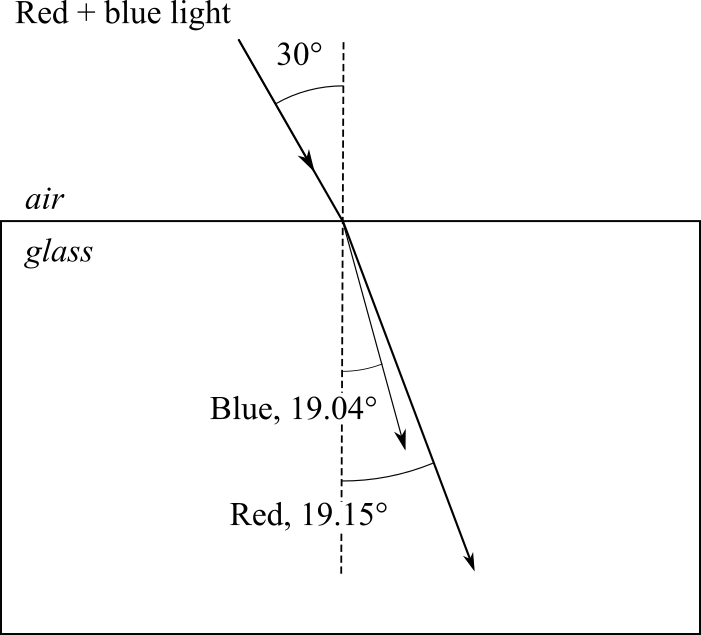
\includegraphics[width=2.338in,height=2.117in]{images/08_debroglie/refraction.png}
    \caption*{\emph{Figure 1: Light beams of different wave-lengths refract at different
    angles in a dispersive medium. (The angular difference is exaggerated in
    this drawing.)}}
  \end{center}
\end{wrapfigure}


Second, Newton had shown that the ``Analogy between colors and
refrangibility is very precise and strict, the Rays always either exactly agreeing
in both or proportionally disagreeing in both.''\footnote{See Newton,
``The New Theory about Light and Colors,'' Prop.\ 2, in the Junior Lab manual.} 
In the wave theory of light, the property of the wave that is
constant when the wave passes from one medium to another is its
frequency, while its speed and wavelength both change. Thus, light of
different frequencies is refracted in different amounts in the same
medium, that is, the index of refraction of light depends on its
frequency.



Whenever the separate colors in white light spread out into a spectrum
upon passing through a prism, it is because waves of different
frequencies are being propagated at different speeds, causing their rays
to bend along different paths. For example, when red light of wavelength
6563 Å shines on the flat surface of a piece of crown glass at an angle
of incidence of 30$^{\circ}$, it will be refracted within the glass at an angle
of 19.15$^{\circ}$ (Fig.\ 1). By Snell's law, the sines of these angles will be in
the same ratio as the speeds of the light in the air and in the glass,
respectively. The frequency remains the same, so the wavelength must
diminish in the glass, in the same ratio in which the speed is reduced.
Thus,
\begin{equation*}
n^{\textrm{red}} = c^{\,\textrm{red}}_{\,\textrm{air}}/c^{\,\textrm{red}}_{\,\textrm{glass}}=\sin 30^{\circ}/\sin 19.15^{\circ}
= \lambda^{\,\textrm{red}}_{\,\textrm{air}}/\lambda^{\,\textrm{red}}_{\,\textrm{glass}}.
\end{equation*}

The speed of light in air, virtually the same as in vacuum, is about
186,000 miles/sec or $3\!\times\!10^{8}$ m/sec---denoted by the letter $c$.
Then, knowing the wavelength of this red light in air, we may calculate
its speed and wavelength in the glass. Similarly, blue light of
wavelength 4861 Å entering the same glass at the same angle will refract
at 19.04$^{\circ}$. At what speed then does this blue light travel in the glass
and what is its index of refraction?

In describing ``the manner how colors are produced by the Prism,''
Newton wrote that ``the Rays [\,\ldots] by their unequal refractions must be
severed and \emph{dispersed} into an oblong form in an orderly
succession from the least refracted Scarlet to the most refracted
Violet.''\footnote{Newton, ``New Theory,'' Prop.\ 9, Junior Lab manual; italics added.} The prism is said to
be a \emph{dispersive medium}, and the phenomenon of spreading-out is
called \emph{dispersion}.

So, in dispersive media for matter waves, the index of refraction would
have to depend on the frequency of the waves, in addition to the
location: $n = n(x,y,z,\nu)$. In the particular case of
spherical symmetry: $n \propto f(\nu)/r$, where
$f$ is some function of $\nu$.

De Broglie first proved the general theorem enunciated below and then
applied it to an electron orbiting the hydrogen nucleus, understood as
analogous to light waves moving in a spherically symmetrical, dispersive
medium:

\begin{quotation}
Now let us suppose that at time $t = 0$ the moving particle
coincides in space with a wave of frequency $\nu$, which propagates
with speed $u = c^2/w$ in the same direction as the
particle. This wave of speed greater than $c$ cannot correspond to
a propagation of energy;\footnote{{[}The product of wave and particle
  speeds has been supposed equal to the speed of light squared.
  Therefore, since the particle speed is certainly less than the speed
  of light, the wave speed must be supposed \emph{greater} than the
  speed of light. But it is a tenet in relativity theory that no actual
  process can transmit energy with a speed greater than that of light;
  so the associated wave ``cannot correspond to a propagation of
  energy.'' Hence de Broglie calls it ``fictional'' above.{]}} we
consider it only as a fictional wave associated with the motion of the
moving particle.

I say that, if at time $t$ = 0 there is agreement of phase between
the {[}guiding{]} wave and the internal {[}vibrational{]} phenomenon of
the moving particle this agreement of phase will continue [\,\ldots].

Let us now pass to the case of an electron describing a closed
trajectory at a uniform speed considerably less than $c$. At time
$t$ = 0 the moving particle is at a point P. The associated fictive
wave, departing then from P and describing the complete closed
trajectory at {[}a constant speed much greater than that of the
electron{]}, catches up with the electron at time $\tau$ and at point
P'.\footnote{{[}``Ondes et Quanta,'' \emph{Comptes rendus} 177
  (1923), 507, in \emph{Recherches d'un demi-siècle} (Paris: Albin
  Michel, 1976). We shall not attempt to follow de Broglie's proof.{]}}
\end{quotation}

After calculating the period of revolution of the electron around its
orbit and the internal phase of the electron upon reaching point P', de
Broglie concluded:

\begin{quote}
It is \emph{almost necessary} to suppose that the trajectory of the
electron is stable \emph{only} if the fictive wave passing at P' finds
the {[}internal vibration of the{]} electron in phase with it. The wave
must be in resonance {[}with the electron's internal vibration{]} over
the length of the trajectory {[}actually followed by any orbiting
electron{]}.\footnote{{[}``Ondes et Quanta,'' \emph{Comptes
  rendus} 177 (1923), 507--508, in \emph{Recherches d'un demi-siècle}
  (Paris: Éds, Albin Michel, 1976). De Broglie's symbols have been
  changed.{]}}
\end{quote}

De Broglie then demonstrated that an equation equivalent to Bohr's
equation \eqref{eq:bohr_8} in Chapter \ref{ch:bohr} above (p.~\pageref{eq:bohr_8})
followed from this ``condition of
stability.'' The general idea is that the requirement of staying in
resonance with the electron's internal vibration around the orbit
restricts the fictive matter waves to a particular set of wavelengths
and also to particular distances from the nucleus, which turn out to be
the same as the radii of Bohr's orbits. By virtue of the de Broglie
relation, $\lambda = h/p$, these allowable wavelengths then
determine the electron's momentum and hence the kinetic energy,
$KE = p^2/2m$, of the system,
leading to the discrete energy values (the potential energy being
inversely proportional to the distance) that Bohr had been forced to
postulate.

For since the electron is circling around the orbit, the ray of the
fictive waves and the fictive waves themselves are also circling upon
themselves around that orbit. Hence, since, by de Broglie's condition of
stability, the internal periodic phenomenon of the electron must remain
in phase with its guiding waves; therefore, those waves, as they
continually superimpose each of their circuits on its previous ones,
\emph{must remain in phase with themselves}. This condition will be met,
however, only if the circumference of the orbit is \emph{equal to} the
de Broglie wavelength, or twice, or three times, or \emph{any}
\emph{integral multiple of the wavelength}.

But this is exactly what happens in the second, or third, or any Bohr
orbit; in general, for the $n$th Bohr orbit, the circumference
$2\pi a_n$ will equal $n\lambda_n$.\footnote{This general result is easy to show
  by adding subscripts to Eq.~(i) of fn.~\ref{fn:bohr_ke} (p.~\pageref{fn:bohr_ke}) and
  Eq.~\eqref{eq:bohr_8} in the main text of Chapter \ref{ch:bohr} (p.~\pageref{eq:bohr_8}). 
  Between equations 
  $mw_n^2 = e^2/a_n$ and $2a_n = n^2h^2/2\pi^2me^2$,  eliminate $e$ to obtain
  $4\pi^2a_n^2 = n^2h^2/m^2w_n^2$. Taking
  square roots then yields $2\pi a_n = nh/mw_n$;
  but since $h/mw_n = \lambda_n$, we see
  that the orbital circumference $2\pi a_n$ is always
  an integral multiple $n$ of the electron's associated wavelength
  for that orbit.

  Thus it was for a time accepted that in-phase overlapping of the
  wavelengths is what determines the eligible orbits of a particle.
  However, this neat result proved to be valid only for hydrogen, and to
  some extent helium. Success with the heavier elements required other
  methods, such as Schrödinger's in Chapter \ref{chap:sch}.} For instance, consider an
electron in the first Bohr orbit of a hydrogen atom. The diameter
$2a_n$ of the $n$th orbit in the hydrogen atom
was shown by Bohr to be\footnote{See Bohr's equation \eqref{eq:bohr_8} in Chapter
\ref{ch:bohr} above (p.~\pageref{eq:bohr_8}).}
%
\begin{equation*}
2a_n = n^2 \cdot \frac{h^2}{2\pi^2me^2}\, \text{cm.}
\end{equation*}
%
Using modern values for electron mass $m = .910\times 10^{-27}$ gm,
electron charge $e = 4.802\times 10^{-10}$ esu, and Planck's constant
$h = 6.625\times 10^{-27}$ erg-sec, we find the radius of the first orbit
($n$ = 1) to be $a_1 = .530\times 10^{-8}$ cm and the
circumference to be $2\pi a_1 = 3.33\times 10^{-8}$ cm. On the
other hand the electron's speed was given by\footnote{See Bohr's
  equation \eqref{eq:bohr_4} and the related footnote (fn.~\ref{fn:bohr_ke})
   in Chapter \ref{ch:bohr} above
  (p.~\pageref{eq:bohr_4}).}
%
\begin{equation*}
mw^2 = \frac{e^2}{a} ,
%
\end{equation*}
which, using the values previously obtained, yields a value for the
electron's orbital speed in the orbit of radius
$a_1, w_1 = 2.186\times 10^8$ cm/sec.

According to de Broglie's relation between particle momentum and
associated wavelength, then, the electron in the first hydrogen orbit
will be associated with a wave of wavelength
\begin{equation*}
\lambda_1 = \frac{h}{mw_1} = \frac{6.625\times 10^{-27}}{.910\times 10^{-27}\cdot2.186\times 10^8}
 = 3.330\times 10^{-8} \text{cm},
\end{equation*}
which is exactly the same length as the circumference of the first Bohr orbit!


On this hypothesis there can be no orbit of the electron between Bohr
orbits \emph{because} its phase wave cannot combine coherently with
itself there. Those intermediate spaces are analogous to the dark bands
in an interference pattern, where the phase waves interfere
destructively. The sketch below is a symbolic representation of the wave
dispositions for the first three orbits of hydrogen, drawn first on
straight paths and then bent around into orbital circumferences. Note
that the depicted shapes of the waves do not accurately represent either
the actual motion of the fictive waves or their associated rays.

\begin{figure}[h] % Figure 2
  \begin{center}
    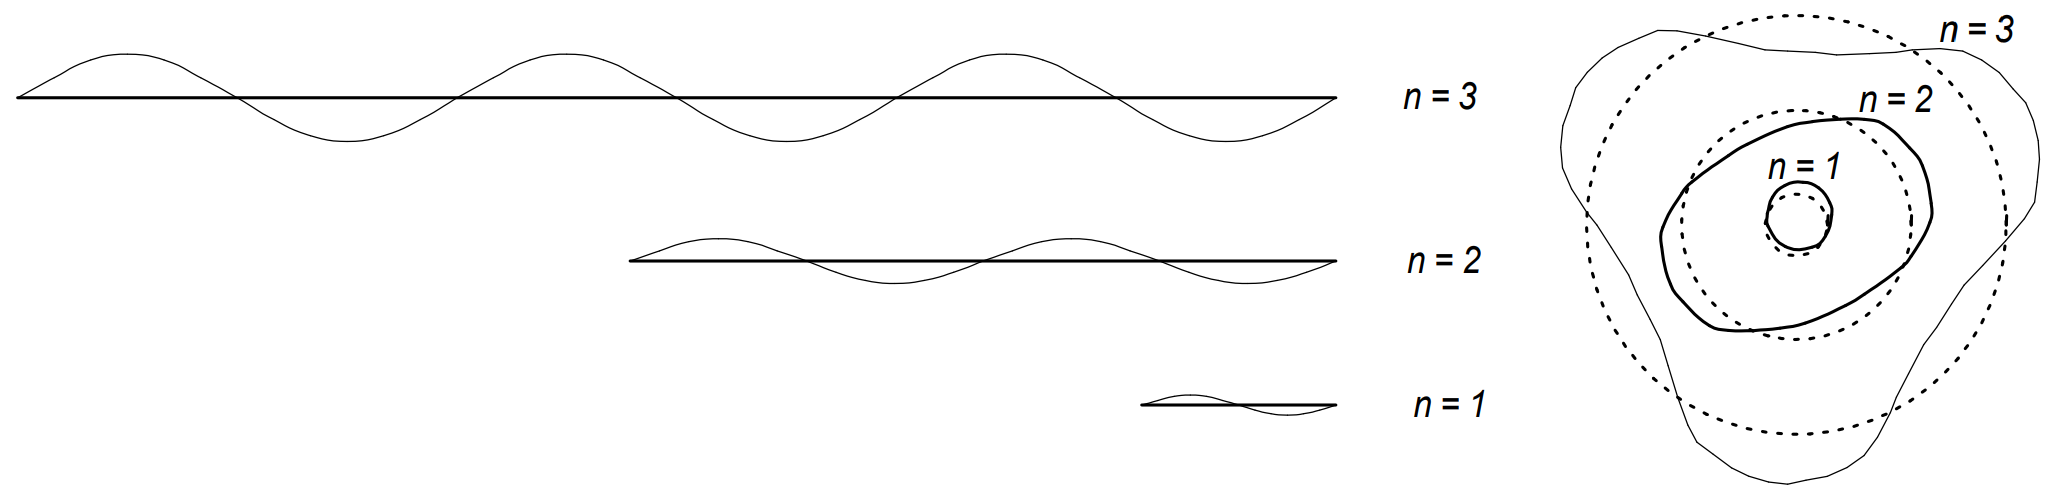
\includegraphics[width=\textwidth]{images/08_debroglie/standing-waves.png}
  \end{center}
  \caption*{\emph{Figure 2: de Broglie wavelengths for the first three Bohr orbits of
     hydrogen. In general the wavelength for the orbit of radius $a_n$ is
     $\lambda_n = 2\pi a_n/n$. (The diagram is not drawn to scale.)}}
\end{figure}



\section*{C. Packets of Matter Waves: Application to the Free Particle }\label{SecC}

In a late work of his, reporting on his point of departure for
developing the idea of matter waves, de Broglie stresses the merely
approximate character of geometrical, or ray, optics\footnote{See fn.~\ref{fn:deb_approx} in
  in Section A above (p.~\pageref{fn:deb_approx}).} and, hence, of the old, Newtonian mechanics:

\begin{quotation}
As early as 1923 I had formulated the fundamental idea that traditional
Mechanics (in both its relativistic and classically Newtonian form) was
only an approximation with the same range of validity as geometrical
Optics. From that moment I was led to realize the necessity of
constructing a new Mechanics, an undulatory Mechanics [\,\ldots].

In every case where Geometrical Optics is sufficient to describe the
propagation of the $\Psi$ wave {[}as the matter wave came to be
designated{]} [\,\ldots] the trajectories, determined by the Classical
Dynamics of a point mass [\,\ldots] will be simply the rays of propagation of
the $\Psi$ wave [\,\ldots].

And thus we arrive at one of the main ideas of the new Mechanics.
Whereas the older Mechanics attributed a rigorous character to {[}the
equations of these trajectories{]} and considered them valid everywhere,
the new Mechanics gives the leading role to the wave. It considers the
equations of the older Mechanics as approximations valid only when the
approximation of Geometrical Optics is sufficient to describe the
propagation of the wave.

Classical Dynamics thus appears to be only an approximation. It is
applicable only when the index {[}of refraction{]} $n$ relative to
the $\Psi$ wave varies only slightly in comparison with a wave-length
or, what is essentially the same thing, when the potential
$V$\footnote{{[}In the case of the orbiting electron, this would be
  the electrical potential of the electric field due to the positively
  charged hydrogen nucleus. That is what causes the trajectory of the
  electron to curve analogously to the way in which an index of
  refraction $n \propto 1/r$ would cause a light ray to curve in a
  circle. We shall see below how it is ``essentially the same
  thing.''{]}} varies slowly over the distance of a wave-length.
However, if the wave-length of the $\Psi$ wave were infinitesimally
small, the older Dynamics would be rigorously valid.\footnote{{[}L. de
  Broglie, \emph{Non-linear Wave Mechanics: A Causal Interpretation}
  (Amsterdam: Elsevier, 1960), 7, 19--20.{]}}
\end{quotation}

Thus far we have not seen how the motion of material particles as
determined by geometrical optics, that is, as being the trajectories, or
rays, determined by the matter waves, is only approximate. For, as
explained in Section B, the Bohr orbits of the electron in the hydrogen
atom appeared to be exact, not approximate. In Section B, however, it
was only claimed that the electron is localized in certain orbits;
nothing was said about its motion around an orbit. The examples
discussed in the 1923 articles did not manifest that approximate
character. Now in order to make clear that the motion of a particle is
not \emph{exactly} the motion determined by geometrical optics, we shall
imagine the motion of a free electron, such as one shot at a screen, as
in the cathode-ray tube. We ask whether there is a wave phenomenon that
moves toward the screen in roughly the same way as does the classical
electron.

To answer this question we follow de Broglie's procedure in his
dissertation,\footnote{The following account is based on his summary
  presentation in L.\ de Broglie, ``On the Parallelism between the
  Dynamics of a Material Particle and Geometrical Optics,'' \emph{op.\
  cit.,} 10--11.} written in 1924. There, in order to establish ``a close
connection between the propagation of the wave and the dynamics of the
associated corpuscle,''\footnote{\emph{Ibid}., 12.} he made use of a
familiar general wave phenomenon, known as a \emph{group} of waves, or a
\emph{wave packet}, which was not studied in Junior Laboratory. A wave
packet might be thought of as a wave phenomenon that concentrates its
energy in a ``burst.'' Many wave phenomena can exhibit ``burst-like''
features. For example, a vibrating string produces a steady tone, but
two strings slightly out of tune also produce ``beats,'' a regular rise
and fall in volume. Similarly, a rock dropped in a pond causes a
distinct \emph{band} of ripples to spread out, rather than a constant
undulation all across the pond.

Take a closer look at the disturbance caused by dropping a rock in a
pond. Within the band, the ripples are moving
just as a train of sine-waves would, except that each ripple
\emph{starts up} or \emph{emerges} at the trailing edge of the
band and \emph{fades out} at its leading edge. The ripples are moving
through the band, at a greater speed than the band itself, but are
noticeably present only inside the band. Consider a patch of water some
distance from the point where the rock is dropped; that patch remains
undisturbed until the band reaches it, which takes longer than the
ripples would if they moved continuously from the rock. In fact, in
water such a band moves at a speed that is only about half that at which
the ripples in it are moving. But the band is nothing but a band of
ripples. The ripples build up a distinct band, but disappear outside it.
This makes sense only if the ripples are actually a sum of component
waves which add up constructively to form the band, but add up
destructively to cancel themselves out outside the band. The band of
ripples is a moving reinforcement, or interference pattern.

Suppose, then, that a particle is accompanied not by one phase wave but
by a collection of them. It is possible that the sum of the phase waves
might produce a wave packet, a single localized region in which that sum
had an amplitude other than zero, while cancelling itself out everywhere
else. Like the band of ripples, the wave packet would move more slowly
than the individual waves within it. The particle could then be thought
of as riding along in the wave packet, as in Figure 3.

\begin{figure}[h] % Figure 3
  \begin{center}
    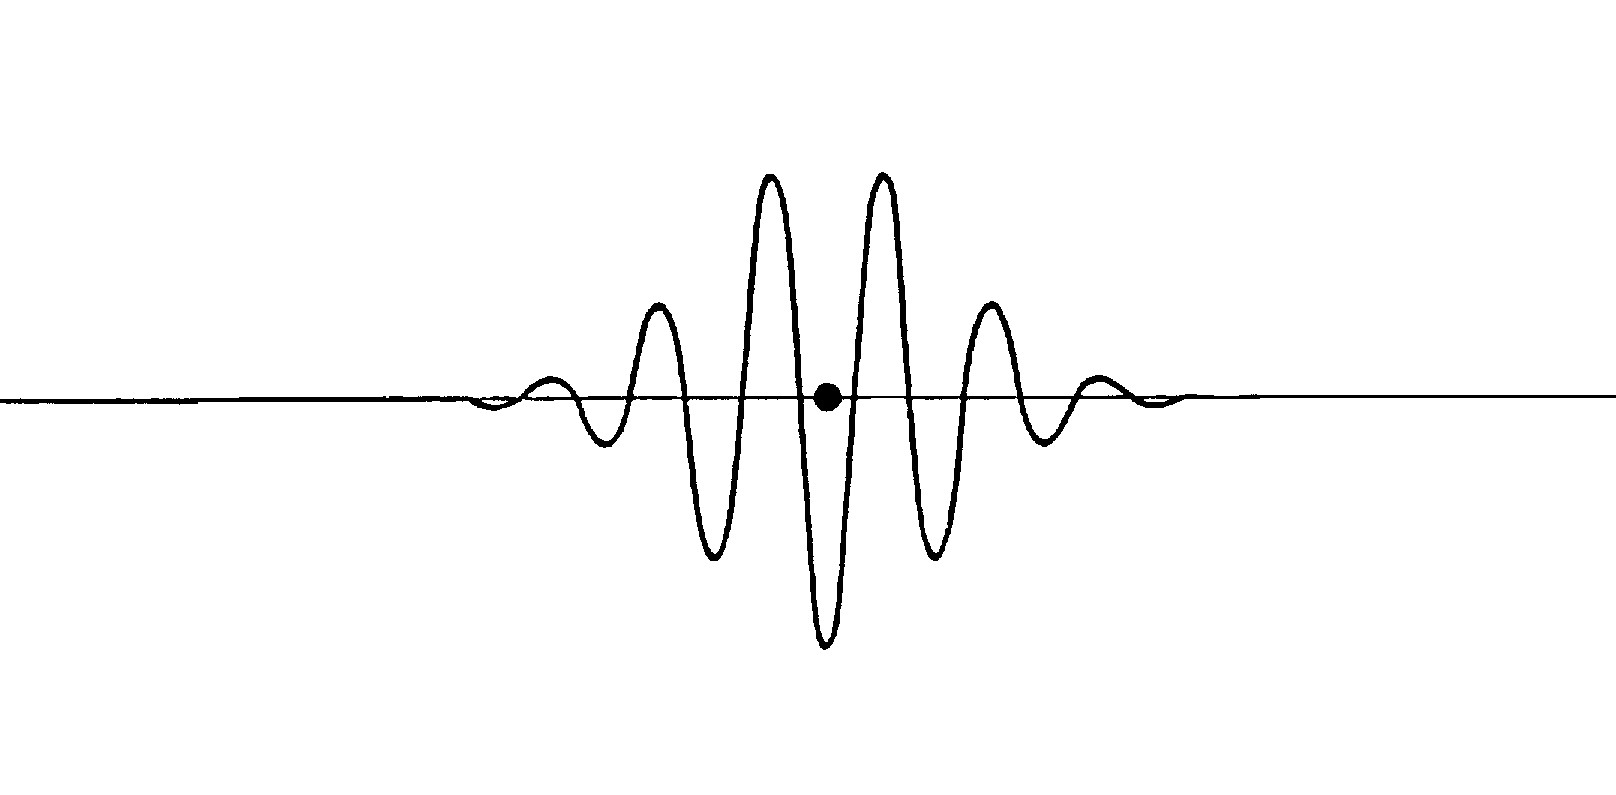
\includegraphics[width=.7\textwidth,height=.34436\textwidth]{images/08_debroglie/pilot.jpg}
  \caption*{\emph{Figure 3}}
  \end{center}
\end{figure}

The speed of a component phase wave is called the \emph{phase velocity}.
The speed of the packet is called the \emph{group velocity}. Now, the
phase velocity is determined by the two de Broglie relations for the
values for the total energy $E$ and momentum $p$ of the
particle, since they determine $\nu$~and $\lambda$,~the product of
which is the phase velocity $u$. The group velocity $g$ of the
wave packet is in turn determined by the mathematics of the addition of
wave functions; however, the particle's velocity $w$ is already
contained in the quantity $p$. The wave packet is a leading
candidate for fulfilling the role of a matter-wave phenomenon that would
move in such a way as to determine the approximate location of the
particle at any time. Hence, if it is to succeed in fulfilling that
role, de Broglie must show that $g = w$. Recall, too, that
in Section A the speeds $w$ and $u$ were assumed inversely
proportional: $wu = c^2$. As we shall see, the mathematics of
wave packets must retain this inverse proportionality between the speeds
$w$ and $u$.

Here are some examples of wave packets in various media. In a simple
wave phenomenon, a disturbance of some amplitude in a medium propagates
at a constant speed. In the simplest case from Junior Laboratory, the
medium is a rope and the disturbance is a displacement up and down of
particles along it, propagating in the one dimension of the string's
extension when we shake it up and down once. When a rock is dropped into
water, the disturbance is again an up-and-down displacement in the
medium of water, but now the propagation is in two dimensions across the
water's surface. A sound wave coming from the striking of a gong
propagates in three dimensions through the medium of air; this is
possible because the displacement of particles is forward-and-back in
the direction of propagation, longitudinal rather than transverse.

In Maxwell's theory of light, a disturbance from the flash of a signal
light is a pulse in electric and magnetic field strengths that is both
transverse and three-dimensional. The material medium, the ether,
postulated by Maxwell was, however, soon rejected as having
contradictory properties; thus the ``medium'' of light remains nothing
but a distribution of potential energy in empty space. An
electromagnetic pulse of light may be understood by analogy to the sound
wave due to the striking of a gong, but with the medium removed and the
amplitudes replaced by oscillating field strengths, transversely
directed and oriented perpendicularly to each other.

The groups of phase waves of wave mechanics take a further step away
from concreteness. They have no material medium, and their amplitudes
are simply assigned the letter $\Psi$. They are groups of $\Psi$
waves in a non-physical medium, which can, however, be characterized by
an index of refraction: $n = n(x,y,z,\nu)$, as we have seen in
Section B. Hence, the medium can be expected to manifest itself by its
effect on the velocity of a wave group.

Before attempting to demonstrate what de Broglie termed the ``Theorem of
Group Velocity,'' namely, that the group velocity equals the particle
velocity: $g = w$, we shall become familiar with the
mathematics of the composition of a group of phase waves in general and
of the determination of the group velocity.

Any function of the form $f(x-ut)$ represents a
configuration that travels with velocity $u$. For consider
$f(z)$, where $z$ is measured from some point that
moves with speed $u$ in the direction of increasing $x$; so
that the graph of $f(z)$ is certainly moving with speed
$u$. But, as Figure 4 shows, $z = x-ut$.
Therefore the graph of $f(x-ut)$ also moves with
speed $u$. It is not necessarily periodic.

\begin{figure}[h] % Figure 4
  \begin{center}
    \captionsetup{width=3.4in}
    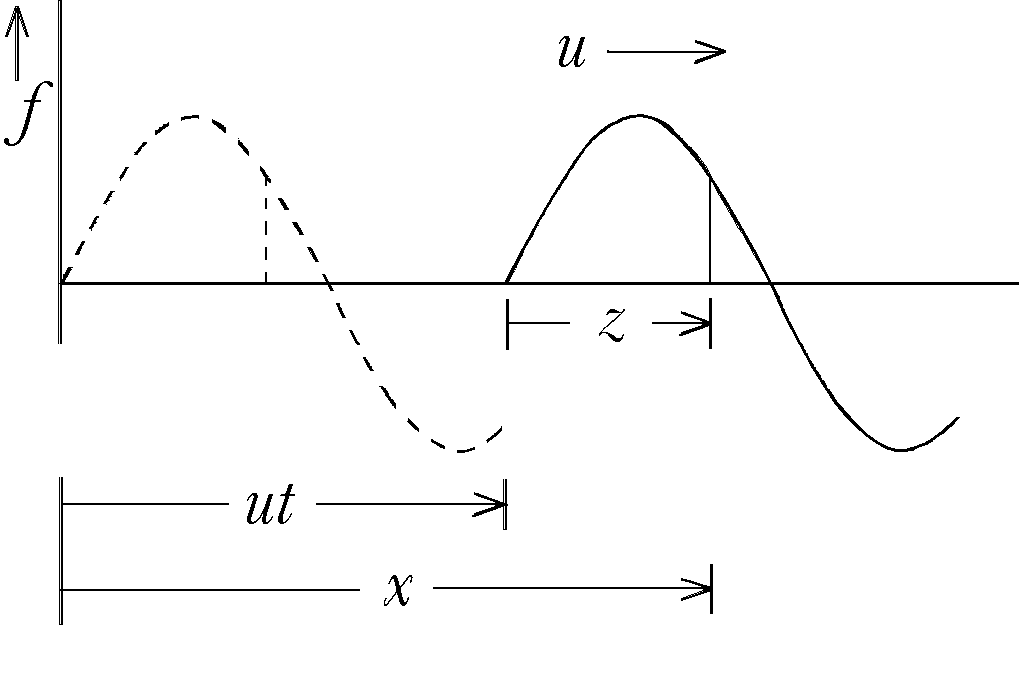
\includegraphics[width=3.4in,height=2.28in]{images/08_debroglie/image025.png}
    \caption*{\emph{Figure 4. The solid curve $f(z)$ moves with speed $u$.
    The dotted curve shows its position at some earlier moment. As the
    drawing shows, $z = x - ut$; and thus
    $f(z)$ is identical to $f(x-ut)$.}}
  \end{center}
\end{figure}

The function
\begin{equation*}
\Psi(x,t) = A \sin 2\pi k(x-ut)
\end{equation*}
not only travels with velocity $u$ as above; it, in addition, shows
periodicity at spatial intervals $\lambda$ such that $2\pi k\lambda = 2\pi$ 
which gives $\lambda = 1/k$ (this is apparent when
$t = 0$), and at time intervals $T$ such that $2\pi kuT = 2\pi$ 
from which it follows that $T = 1/ku$ (apparent
for $x = 0$). $\lambda$ is the \emph{wavelength}, and $T$ is
called the \emph{period}. The quantity \emph{k}, the inverse of
the wavelength, is called the \emph{wave number} (it is the
\emph{number} of wavelengths per unit distance). The quantity $A$
is the \emph{amplitude}, the maximum ``height'' of the wave disturbance.

When written as above, namely
\begin{equation*}
\Psi(x,t) = A \sin 2\pi k(x-ut)
\end{equation*}
the traveling wave may be said to be expressed in \emph{velocity} form,
inasmuch as it shows the velocity $u$ explicitly.

The frequency is the inverse of the period; that is, variously
expressed:
\begin{equation*}
\nu = 1/T = ku = u/\lambda .
\end{equation*}
With these substitutions, the traveling, periodic wave given above may
also be written in the form
\begin{equation*}\tag{1}
\Psi(x,t) = A \sin 2\pi(kx-\nu t)
\end{equation*}
which may be called the \emph{frequency} form; it shows the frequency
$\nu$ explicitly. Although the wave velocity is not here overtly
expressed, it will be clear from the preceding that $u = \nu\lambda = \nu/k$.

Each of de Broglie's phase waves must obey, in any one dimension,
Equation (1). To see how a wave packet is composed, let us add two waves
that differ slightly in frequency and wavelength. If
\begin{equation*}
\Psi_1  = A\sin 2\pi(kx-\nu t)\quad\text{and}\quad\Psi_2 = 
A\sin 2\pi((k+\Delta k)x - (\nu + \Delta\nu)t),
\end{equation*}
then their sum\footnote{A crucial trigonometric identity for much of
  what follows is: 
  \begin{equation*}
  \sin a + \sin b = 2 \sin\left(\frac{a+b}{2}\right)\cdot\cos\left(\frac{a-b}{2}\right).
  \end{equation*}
  It can be derived, with some labor, from the better-known identities $\sin{(a+b)} = 
  \sin a\cos b + \cos a\sin b$
  (and the special case in which $\sin{2a} = 2\sin{a}\cos{a}$) and
  $\cos{(a-b)} = \cos{a}\cos{b} + \sin{a}\sin{b}$.} is
\begin{equation*}
\Psi_{1+2} = 2A\cos 2\pi\left(\frac{\Delta k}{2}x - \frac{\Delta\nu}{2}t\right)
\cdot \sin 2\pi\left(\frac{k+(k+\Delta k)}{2}x - \frac{\nu+(\nu+ \Delta\nu)}{2}t\right).
\end{equation*}

We have manipulated this equation algebraically to bring out its formal
resemblance to Equation (1). The sine factor here corresponds to the sine
factor in Equation (1), but here the coefficient of $x$ is the
average of $k$ and $k + \Delta k$, while the coefficient of
$t$ is the average of $\nu$ and $\nu + \Delta\nu$; thus the
sine factor represents a wave whose wave number is the average of the
two component wave numbers and whose frequency is the average of the two
component frequencies.

The amplitude $A$ in Equation (1) corresponds here to the whole
factor 
%
\begin{equation*}
2A\cos 2\pi\left(\frac{\Delta k}{2}x - \frac{\Delta\nu}{2}t\right) , 
\end{equation*}
%
which thus plays the role of a \emph{variable} amplitude, the
\emph{envelope}. The maximum value of the envelope is $2A$, which
is twice the amplitude $A$ of either component. This indicates that
the sum of the two waves attains a maximum wherever two crests or two
troughs of the component waves add up. Since the envelope also involves
a cosine term, and since the cosine exhibits the same wavelike shape as
the sine, the envelope can itself be viewed as a wave: its wave number
will be half the difference of the component wave numbers, and its
frequency will be half the difference of the component frequencies. The
compound wave formed by adding two components thus seems to be acting
like a wave in two ways at once (see Figure 5).

\begin{figure}[h] % Figure 5
  \begin{center}
    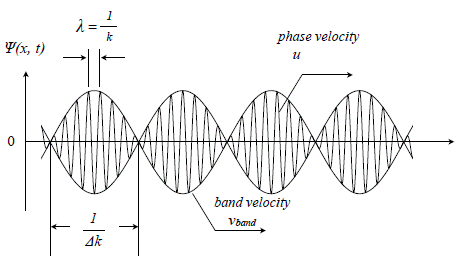
\includegraphics[width=4.90625in,height=2.85417in]{images/08_debroglie/image036.png}
    \caption*{\emph{Figure 5}}
  \end{center}
\end{figure}

In the figure the dense inner line graphs the sine factor. Its wavelength is
labeled as $\lambda = 1/k$. This is approximately true: since
$\Delta\lambda$ was chosen to be small, the wavelength of $\Psi_2$ differs
little from $\lambda$, the wavelength of $\Psi_1$, and the average of
the two wavelengths differs from it even less. The speed of propagation
of the inner-line wave is the phase velocity $u$. The more relaxed
outline graphs the cosine factor, the envelope surrounding the
higher-frequency wave. The graph also shows the meaning of the two factors in
the expression for $\Psi_{1+2}$: the compound wave is a wave within a
wave. Thus two component waves of slightly different frequencies and
wavelengths will combine to form an interference pattern consisting of a
succession of bands enveloping or containing a wave of shorter
wavelength and higher frequency.

This is not quite where we want to be, since the envelope is an endless
string of adjacent bands rather than a single isolated wave packet.
Nevertheless, it permits us to form a simple equation deriving the
velocity of any band in the envelope---which could be viewed in
isolation as a group formed of two component phase waves---from the
properties of its two component phase waves. Since the speed of any wave
in general is the product of its wavelength and frequency, and since we
can read these values \emph{for any band} from the coefficients in the
cosine factor, the band velocity, $u_{\,\text{band}}$, may be
expressed as
\begin{equation*}\tag{2}
u_{\,\textrm{band}} = (\text{wavelength})\times (\text{frequency}) = \frac{2}{\Delta k}\frac{\Delta\nu}{2} = 
\frac{\Delta\nu}{\Delta k}
\end{equation*}

Figure 6 shows how the two component waves build up the compound
envelope and its bands. The two components are shown in a ratio of
wavelengths of $9:8$. At (a), crests of the longer and the shorter wave
coincide to produce a maximum in their sum. Then at (b), after 4 full
cycles of the longer and $4-\frac{1}{2}$ of the shorter, a crest of the longer
component coincides with a trough of the shorter one, producing a node
in the compound wave. At (c) both components display crests again,
producing a maximum in their sum once more. Each repetition of the same
interval brings the two components back out of phase 180$^{\circ}$ at a node, or
back in phase at a common crest.

\begin{figure}[h] % Figure 6
  \begin{center}
    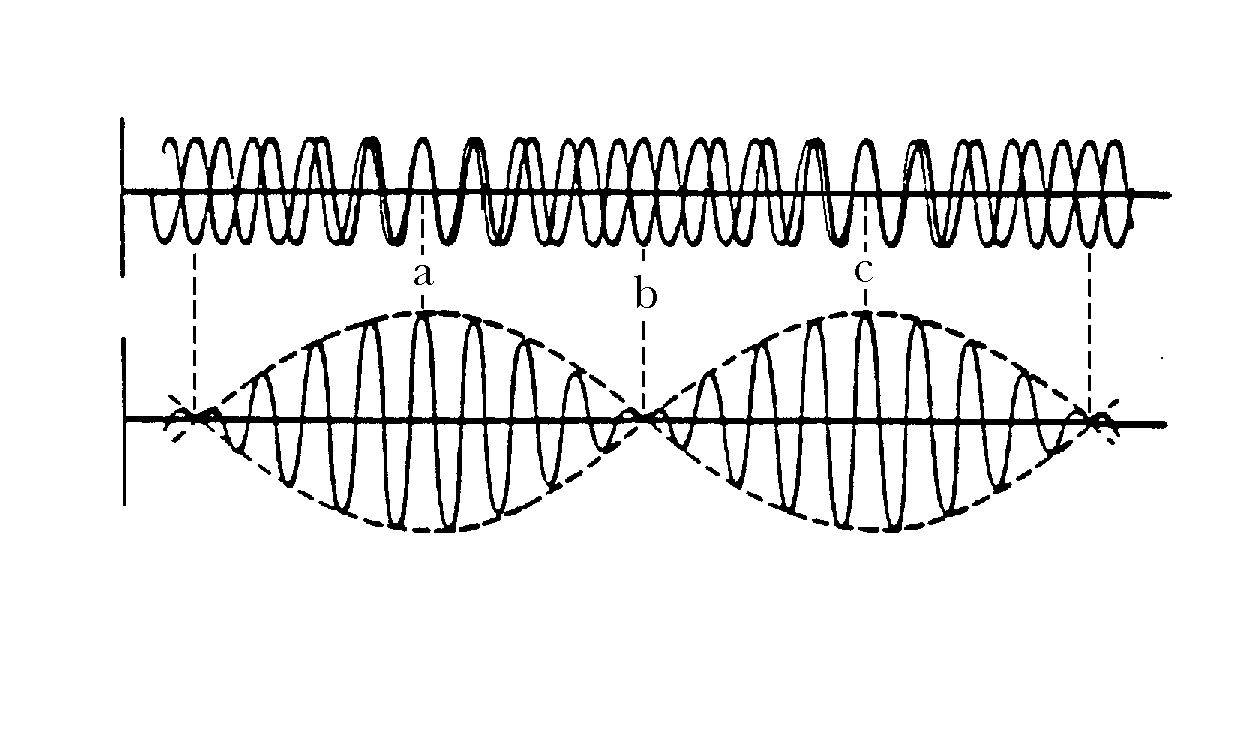
\includegraphics[width=4.18333in,height=2.51667in]{images/08_debroglie/image039.png}
    \vspace{-3em}
    \caption*{\emph{Figure 6}}
  \end{center}
\end{figure}

The pattern in Figure 6 must continue indefinitely. But what happens if
we add a third component wave with a wavelength and frequency between
those of the first two components? If we add a fourth? A fifth?
Infinitely many? Figure 7 may suffice to answer these questions in a
general way. It shows a sum of six component waves. The envelope will
clearly have its maximum amplitude at every point where all the
components reach a crest together, and these points will also be the
centers of the bands. But each additional component wave increases the
distance between the centers of bands. To see why, look once more at
Figure 6.

\begin{figure}[h] % Figure 7
  \begin{center}
    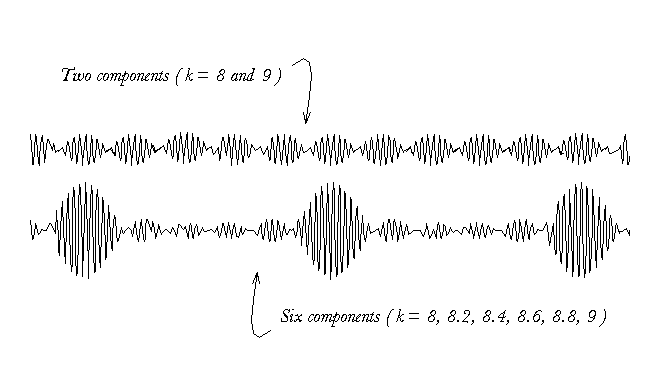
\includegraphics[width=4.35334in,height=2.52in]{images/08_debroglie/image041.png}
    \caption*{\emph{Figure 7. Six component waves of the indicated wave numbers, two of
     which are shown on top, are added to produce more widely separated bands
     of greater amplitude.}}
  \end{center}
\end{figure}

There, a third component with a wavelength halfway between the two shown
would cycle $8-\frac{1}{2}$ times between (a) and (c). If the third component were in
phase with the first two at (a), then it would be out of phase with them
at (c) and would subtract its amplitude from their sum. With proper
choice of amplitudes, every second maximum could be nearly canceled; the
distance between adjacent common maxima of all three components would
then be double the distance for the first two alone. So by adding ever
more intermediate component waves---canceling out every third, fourth,
fifth maximum, and so on---we can eventually move the centers of
adjacent bands as far apart as we please.

Does each band stretch to fill the longer interval? Figure 7 suggests
that it does not, but that instead the envelope cycles up and down near
the baseline between bands that themselves remain narrow. As more and
more intermediate component waves are added and the common crests become
fewer and farther between, there are also more and more opportunities
for every component at every spot in between to have an amplitude nearly
equal and opposite to that of some other component; so that the
amplitude of the envelope will fall off rapidly on both sides of each
maximum, and tend everywhere else toward zero.

This suggests, and it can in fact be proved, that if we added a
countable infinity of suitably selected\footnote{The infinity of values
  of $k$ between 8 and 9 must be everywhere dense on the interval
  {[}8,9{]}; that is, given any one of them, it must be impossible to
  find an interval containing it that does not also contain
  another---and, in fact, an infinity---of the selected points in its
  interior.} intermediate component waves while focusing our attention
on a single band, the other bands would be removed to an infinite
distance, leaving the single wave packet of Figure 3. This claim is
analogous to that of Daniel Bernoulli that ``all sonorous bodies contain
potentially an infinity of sounds, and an infinity of corresponding ways
of making their regular vibrations.''\footnote{D.\ Bernoulli, ``Reflections and Elucidations 
on the New Vibrations of Strings'', par.\ IV, Junior Lab manual.

In fact, given any ``reasonable'' finite curve represented by a function
  $f(x)$ on an interval $(0,L)$, and such that $f(0) = 0
  = f(L)$, we may determine the constants
  $A_n$ such that the curve is represented by an
  infinite sum of sinusoidal curves: 
  \begin{equation*}
  f(x) = \sum_{n=1}^{\infty}A_n \sin (n\pi x/L). 
  \end{equation*}
  We could
  imagine $f(x)$ as representing a snapshot of the top half
  of a wave packet at any time. Similarly, if $g(x,t)$ is a
  ``reasonable'' function, which here represents the forward motion of
  the top half of a wave packet, then it is possible to determine the
  constants $B_n$ such that $g$ may be
  represented as a sum of an infinite number of standing waves (compare
  Bernoulli, ``Reflections,'' par.\ XII):
  \begin{equation*}
  g(x,t) = \sum_{n=1}^{\infty} B_n \sin (n\pi x/L) \cos (2\pi\nu t).
  \end{equation*}
  }

To keep the amplitude of the packet finite, while adding infinitely many
increments to it, we could, for example, let the amplitudes of the
outermost components each be $1$, that of the central one $1/2$, those of
the two halfway between the central and outermost ones $1/8$, etc.---the
amplitude of the packet would then be
\begin{equation*}
2 + 2^0\cdot(1/2)^1 + 2^1\cdot(1/2)^3 + 2^2\cdot(1/2)^5 + \cdots = 3.
\end{equation*}
In this way we could construct an envelope that is a single wave packet rather
than an infinite series of bands. The same reasoning that led to Equation (2) for
the bands in an envelope now applies to an envelope of only one band.
Hence, we have for the velocity of the packet, the group velocity:
\begin{equation*}\tag{3}
g = \frac{\Delta\nu}{\Delta k}.
\end{equation*}

The exact way in which the group would move depends on its index of
refraction. Even though this medium in which the $\Psi$ waves move is
unknown, it can be characterized in one way by its effect on the speed
of the waves. For just as in empty space (index of refraction constant:
$n = 1$) all electromagnetic waves, whatever their frequency, move
at the same speed $c$, so, if the index of refraction were the same
for $\Psi$ waves of different frequencies, then every component phase
wave in a group would have the same speed $u$. Under this
condition, the phase velocity would also have to be equal to this
constant $u$. What would the group velocity then be? Since
\begin{equation*}
k = \frac{1}{\lambda} = \frac{\nu}{u},
\end{equation*}
therefore, where $u$ is a constant,
\begin{equation*}
g = \frac{\Delta\nu}{\Delta k} = \frac{\Delta\nu}{\Delta(\nu/u)} =
\frac{\Delta\nu}{\Delta\nu/u} = u\frac{\Delta\nu}{\Delta\nu} = u,
\end{equation*}
and the wave packet would move with the same speed as the compound phase
waves within it. But we want the packet to keep pace with the particle
at speed $w$, which must be inversely proportional to $u$.

Already in Section B, in order to derive the Bohr orbits from matter
waves, we saw that de Broglie had supposed that the index of refraction
for them depended on both location and the frequency of the waves:
$n = n(x,y,z,\nu)$, that they moved in a dispersive medium.
Now we shall prove that the two de Broglie relations $E =h\nu$ and 
$p = h/\lambda$ imply that the $\Psi$ waves
\emph{are} subject to dispersion. For,
\begin{equation*}
u = \nu\lambda = \frac{E}{h}\frac{h}{p} = \frac{E}{p} = \frac{h\nu}{p}.
\end{equation*}
And
\begin{equation*}
p = mw = \sqrt{m^2w^2} = \sqrt{2m\cdot\frac{mw^2}{2}} = \sqrt{2m(E-V)}
= \sqrt{2m(h\nu - V)},
\end{equation*}
where the total energy of the particle minus its potential energy $(E - V)$ has
been substituted for its kinetic energy. Substitution of the above
expression for $p$ into the equation for $u$ gives\footnote{$V$ here is potential energy. If $E$ is substituted
  for $h\nu$ in Eq.~(4), the resulting equation,
  \begin{equation*}
  u = \frac{E}{\sqrt{2m(E-V)}}
  \end{equation*}
  is identical to Schrödinger's Equation \eqref{SchDeB}, page \pageref{SchDeB}. There he
  develops a differential equation for the $\Psi$ waves like that for
  the vibrating string. Then by assuming that his Eq.\ \eqref{SchDeB} is a
  solution to this differential equation, he is able to determine a
  time-independent differential equation for the part, designated
  ``$\psi$,'' of the $\Psi$-waves that represents a standing wave.}
\begin{equation*}\tag{4}
u = \frac{h\nu}{\sqrt{2m(h\nu -V)}}.
\end{equation*}
Now, since $V=V(x,y,z)$, therefore, by Equation (4),
the speeds, $u$, of the matter waves depend on their location and
on their frequency, $u = u(x,y,z,\nu)$. Since
the index of refraction is inversely proportional to the speed of the
waves,\footnote{See fn.~\ref{fn:deb_ref} above (p.~\pageref{fn:deb_ref}).}
 this implies that $n = n(x,y,z,\nu)$ and that 
the matter waves do move in a dispersive
medium, as de Broglie had supposed. Just as the index of refraction of a
glass prism disperses light waves of different frequencies, so the
dependence of the wave-speed $u$ on the potential $V$ and on
the frequency of the waves is responsible for the dispersion of the
$\Psi$ waves.

In this case the group velocity, $g$, will \emph{not} turn out to
be equal to the velocity, $u$, of the component waves as happened
above when we had supposed an index of refraction that was independent
of the frequency. Instead the phase waves will ripple through the wave
packet, leaving it behind. Recall that according to Equation (3) the wave
packet will move with speed, $g = \Delta\nu/\Delta k$. Now, since
$k = 1/\lambda = \nu/u$, therefore,
$\nu = ku$, so that $\nu$ is a function of $k$.
Therefore, $\nu$ may be differentiated with respect to $k$, and
as $\Delta k$ tends toward zero, $\Delta\nu/\Delta k$ will approach the
derivative of $\nu$ with respect to $k$.\footnote{\label{fn:deb_range} Although the
  domain of definition of the function $\nu(k)$ is not a
  continuous interval, the fact that it is a countably infinite,
  everywhere dense subset of an interval allows its derivative to be
  defined in the same way as was done in Junior Mathematics.

  When there are only \emph{two} components differing by $\Delta\nu$ and
  $\Delta k$ the expression $g = \Delta\nu/\Delta k$ is exact. When
  there is an infinity of component waves, the expression for group
  velocity is $g = d\nu/dk$, as the next equation states. This
  expression, too, is exact.

  Like any derivative $d\nu/dk$ must be evaluated at individual
  values of the independent variable. The resulting value for $g$
  will depend on whatever value is specified for the wave number
  $k$. Then, inasmuch as the wave packet comprises a \emph{range}
  for $\lambda$ and therefore for $k$, the packet may exhibit a
  corresponding \emph{range} of velocities. This is the result not of
  approximation but of heterogeneity: we cannot get a more sharply
  defined velocity for the packet as a whole by any limiting procedure.}
This yields
\begin{equation*}\tag{5}\label{debsch}
g = \frac{d\nu}{dk} ,
\end{equation*}
which, de Broglie specifies, is to be evaluated at a value of $k$
such that $\nu = E/h$ (he conceives of this as the
central frequency of the component waves).

This group velocity, $g$, is related to the particle velocity,
$w$, through the de Broglie relation $\lambda = h/p$
or $k = p/h$. Here $k$ is a function of
$p$, the momentum of the particle, and, clearly, $dk/dp=1/h$.
Taking Equation (5) and multiplying equals by equals gives
\begin{equation*}
g\frac{1}{h} = \frac{d\nu}{dk}\frac{1}{h} = \frac{d\nu}{dk}\frac{dk}{dp}.
\end{equation*}
Then by the Chain Rule,
\begin{equation*}
g\frac{1}{h} = \frac{d\nu}{dp}.
\end{equation*}
Multiplying both sides by the constant $h$,
\begin{equation*}
g = h\frac{d\nu}{dp} = \frac{d(h\nu)}{dp} = \frac{dE}{dp}.
\end{equation*}
This equation expresses the group velocity of the wave packet in terms
of $E$ and $p$, the total energy and the momentum,
respectively, of the particle.

At this point we can prove de Broglie's Theorem of Group
Velocity:\footnote{L.\ de Broglie, \emph{Non-linear Wave Mechanics: A
  Causal Interpretation} (Amsterdam: Elsevier, 1960), 24.}
\emph{If a group of $\Psi$ waves is associated with the motion of a particle,
and if the central frequency of the group corresponds to the total
energy of the particle, then the group-velocity will be equal to the
particle's velocity.} For we have just seen that $g = dE/dp$. But the total 
energy equals the kinetic energy plus the
potential energy. Further, $p = mw$, so that
$p^2 = m^2w^2$ and thus the kinetic
energy $K$ can be written as $p^2/2m$;
substituting gives
\begin{equation*}
\frac{dE}{dp} = \frac{d}{dp}\left(\frac{p^2}{2m} + V\right).
\end{equation*}
Furthermore, the potential energy $V$ is a function of the spatial
coordinates only, so it acts like a constant when one differentiates
with respect to $p$; and $1/2m$ is simply a constant. Thus,
\begin{equation*}
\frac{d}{dp}\left(\frac{p^2}{2m}+V\right) = \frac{1}{2m}\left(\frac{d}{dp}(p^2)+0\right) = \frac{1}{2m}2p.
\end{equation*}
And in turn
\begin{equation*}
\frac{1}{2m}2p = \frac{mw}{m} = w ;
\end{equation*}
And, therefore,
\begin{equation*}
g = \frac{dE}{dp} = w.
\end{equation*}
When $E$ equals the total energy of a particle, and the central
frequency of the group corresponding to it equals $E/h$, then the
group velocity equals the velocity of the particle. Q.E.D.

Thus, in a dispersive medium the wave packet travels with the same speed
as the particle and transports the particle's energy---simply as a
result of the laws of wave propagation. But this rose has a thorn. The
very fact of dispersion that allows the wave packet to form also forces
it to disperse; the leading edge of the packet will always be moving at
a greater speed than its trailing edge.\footnote{It can be shown that
  (as one might expect) the leading edge will move with approximately
  the greatest velocity in the range mentioned in fn.~\ref{fn:deb_range} above, and the
  trailing edge with approximately the least. We cannot go into the
  details.} The wave packet can supply everything that was classically
attributed to the Newtonian particle except permanence of location.

\section*{D. The Interpretation of Matter Waves}

So far matter waves have been presented as guiding material particles.
Whereas at first de Broglie had viewed the matter wave properties of
wavelength and frequency as \emph{due to} the material particle's
momentum and energy, respectively, in his exposition in English of the
ideas he developed for his dissertation, he proposed that matter waves
are \emph{responsible for} the dynamical properties of material
particles:

\begin{quote}
I shall adopt a point of view slightly different from those which I have
developed up to now, \emph{for I shall take the laws of wave propagation
as fundamental, and seek to deduce from them, as consequences which are
valid in certain cases only, the laws of the dynamics of a
particle.}\footnote{{[}L.\ de Broglie, ``On the Parallelism between the
  Dynamics of a Material Particle and Geometrical Optics,'' \emph{op.\ 
  cit.}, 11--12.{]}}
\end{quote}

From this point of view, the particle would not only have wave
properties; every property of the particle would be given to it by its
accompanying wave.

De Broglie was hardly the only physicist to wonder about the physical
interpretation that should be given to the mathematical formalism of
wave mechanics. As we will see in subsequent chapters, different
thinkers have produced different ways to think about the apparent
paradoxes that arise from trying to find common ground between the
formal mathematics that applies to particles and the formal mathematics
that applies to waves. And there are many more attempts than the ones we
will consider.

The question of how best to understand matter waves is still an open one
today.


\section*{Examples and Exercises with Matter Waves}

1. If every particle is accompanied by a phase wave, why are wave
effects not always evident? Consider Rutherford's experiment: a beam of
alpha particles passes through gold foil, which is a lattice of
regularly spaced atoms, with gaps between nuclei on the order of
$10^{-8}$ cm.

Since the alpha-particle is a charged helium atom, its mass will be four
times that of the hydrogen atom. At the very end of Chapter \ref{ch:millikan}
we found the mass of the hydrogen atom to be 
$1.674\times 10^{-24}$ gm.\footnote{See page \pageref{s:millikan_hyd}.}
Thus the alpha particle has mass $m = 6.696\times 10^{-24}$ gm. And in 
Chapter \ref{ch:rutherford} Rutherford cites the
velocity of the alpha particle as $v = 2.09\times 10^{9}$ cm/sec.\footnote{See
page \pageref{s:rutherford_alpha}.} Then 
the wavelength associated with these
alpha particles must be, by de Broglie's relation,
\begin{equation*}
\lambda = \frac{h}{p} = \frac{h}{mv} = 
\frac{6.625\times 10^{-27}}{6.696\times 10^{-24}\cdot2.09\times 10^9}
= 4.73\times 10^{-13}\, \text{cm}.
\end{equation*}
Thus the phase wave associated with the alpha particle has a wavelength
some $100,000$ times smaller than the $10^{-8}$ cm ``slit''
through which it must pass between the gold atoms. This would be
comparable to a beam of yellow light, wavelength $5900\!\times\!10^{-8}$ cm, passing
through a slit $5.9$ cm wide---for the $100,000:1$ ratio is the same in both
cases. As we would not expect detectable diffraction in the optical
case, neither would discernible diffraction effects be expected in the
scattering of alpha-particles by gold foil.\footnote{For diffraction of
  light of wavelength $\lambda$ by a single slit of width $d$, the
  maximum separation of interference bands will be given by the formula
  $\sin{\theta} = \lambda/d$. (See Note on single-slit diffraction in Chapter
  \ref{ch:heisenberg} below, p.~\pageref{eq:diffraction}.) With
  $\lambda/d$ approximately equal to 1/100,000, the angular
  separation $\theta$ will only be about $.0005^{\circ}$.}

2. What is the wavelength associated with a $200$ g baseball traveling at
$4000$ cm/sec (about $89.5$ mph), in comparison with a $100$-cm-wide doorway?
In this case, $\sin{\theta}$ is on the order of $10^{-34}$,
and the first bands of the interference pattern are separated from the
center by about $10^{-33}$ (one millionth to more than the
fifth power!) degree. The matter waves of perceptible bodies produce no
perceptible effects. If one angstrom ($10^{-8}$ cm) is the
smallest slit-width available, then even something as small as an alpha
particle would have to be moving impossibly slowly to interact
detectably with the opening. On the other hand, the very small mass of
the electron makes it a promising candidate to have a discernible
wavelength.

3. Calculate the wavelength of the phase wave of the electrons in
Thomson's cathode ray experiment, for which Thomson in Chapter \ref{ch:thomson}
tabulated a speed of $2.8\times 10^{9}$ cm/sec.\footnote{See page \pageref{tbl:thomson_air}.}

Using the values already cited, we have
\begin{equation*}
\lambda = \frac{h}{p} = \frac{h}{mv} = 
\frac{6.625\times 10^{-27}}{.910\times 10^{-27}\cdot2.8\times 10^9}
=2.6\times 10^{-9}\, \text{cm}.
\end{equation*}
Calculate the angular separation of the first bright bands produced by
passing the electron beam through a crystal lattice of atoms spaced at
intervals of 5 angstroms $(5\times 10^{-8} \text{cm})$.

We shall have
\begin{equation*}
\sin{\theta}=\frac{\lambda}{d}=\frac{2.6\times 10^{-9}}{5\times 10^{-8}}
= .052
\end{equation*}
which gives an angular separation of nearly $3$ degrees. Diffraction
effects of this size will certainly be detectable---if one knows one is
looking for them!

\chapter{Four Lectures on Wave Mechanics}
\chapterprecis{Erwin Schr{\"o}dinger}

\makeoddhead{myheadings}{\emph{Schr{\"o}dinger}}{}{\thepage}
\makeevenhead{myheadings}{\thepage}{}{\emph{Four Lectures on Wave Mechanics}}

\renewcommand{\theequation}{\arabic{equation}}

\newenvironment{rcases}
  {\left.\begin{aligned}}
  {\end{aligned}\right\rbrace} % for eqn (14')

\section*{First Lecture\footnote{[London: Blackie \& Sons,
  Ltd. (1928) and New York: Chelsea (1982). Our excerpt includes only the first lecture.]}}

\subsection*{1. Derivation of the fundamental idea of wave mechanics from Hamilton's
analogy between ordinary mechanics and geometrical optics.}

\begin{figure}[h] % Figure 1
  \begin{center}
    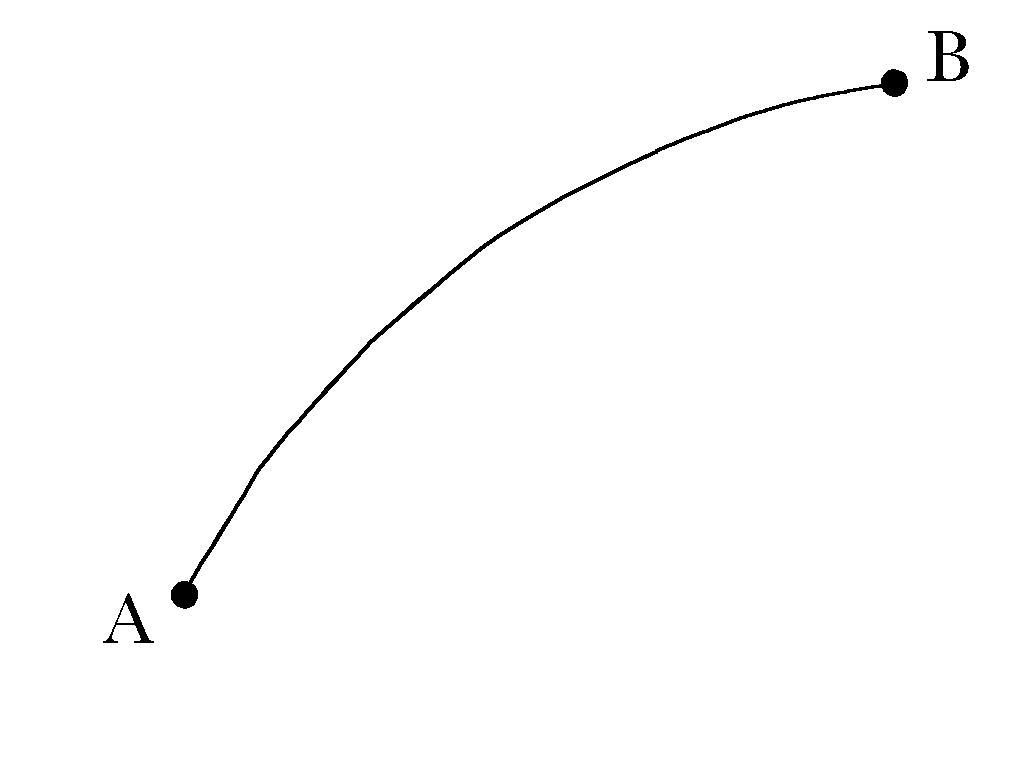
\includegraphics[width=1.98958in,height=1.47917in]{images/09_schroedinger/image035.png}
  \end{center}
  \caption*{\emph{FIGURE 1}}
\end{figure}

When a \emph{mass-point} $m$ moves in a conservative field of
force,
described by the potential energy
$V(x,y,z)$, then, if you let it
start from a given point $A$ with a given velocity, i.e.\ with a given
energy $E$, you will be able to get it into another arbitrarily
chosen point $B$ by suitably ``aiming,'' i.e.\ by letting it start in a
quite definitely chosen \emph{direction}. There is in general \emph{one}
definite dynamical orbit which leads from $A$ to $B$ \emph{with a
given energy}. This orbit possesses the property that
\begin{equation}
\delta \int_{A}^{B} \! 2T\,dt = 0 , % eqn (1)
\end{equation}
and is defined by this property (Hamilton's principle in the form given
to it by Maupertuis). Here $T$ means the kinetic energy of the mass-point,
and the equation means: consider the manifold of \emph{all} orbits
leading from $A$ to $B$ and subject to the law of conservation
of energy ($T + V = E$); among them the actual
dynamical orbit is distinguished by the fact that, \emph{for it} and for
all infinitely adjacent orbits of the manifold, the $\int_{A}^{B}$ has the \emph{same}
value[\ldots]. Calling $w= ds/dt$ the velocity of the mass-point, we have
\begin{equation*}
2T = mw^2 = m\left(\frac{ds}{dt}\right)^2 = 2(E-V) = \frac{ds}{dt}\sqrt{2m(E-V)}
\end{equation*}
by means of which equation (1) can be transformed into
\begin{equation} % eqn (2)
\delta \int_{A}^{B} \! \sqrt{2m(E-V)}\,ds = 0.\footnote{{[}This is equivalent to $\partial \int_{A}^{B} \! mw\,ds = 0$, since $2m(E-V)=2mT=m^2w^2$.}
\end{equation}
This form has the advantage that the variational principle is applied to
a purely geometrical integral, which does not contain the time-variable,
and further, that the condition of constant energy is automatically
taken care of.

\emph{Hamilton} found it useful to compare equation (2) with
\emph{Fermat's} principle, which tells us that in an optically
non-homogeneous medium the actual light rays, i.e.\ the tracks along
which energy is propagated, are determined by the ``law of minimum
time'' (as it is usually called).

Let fig.~1 \emph{now} refer to an optical medium of arbitrary
non-homogeneity, e.g.\ the earth's atmosphere; then, if you have a
searchlight at $A$, furnishing a well-defined beam, it will in
general be possible to illuminate an arbitrarily chosen point $B$
by suitably \emph{aiming} at it with the searchlight. There is one
definite light-path leading from $A$ to $B$, which obeys, and
is uniquely defined by, the law
\begin{equation}
\delta \int_{A}^{B} \! \frac{ds}{u} = 0.
\end{equation}
Here \emph{ds}, as before, means the element of the path, and $u$
is the velocity of light, a function of the co-ordinates $x, y, z$.

The two laws contained in equations (2) and (3) respectively become
\emph{identical}, if we postulate that
\begin{equation}
u = \frac{C}{\sqrt{2m(E-V)}} % eqn (4)
\end{equation}
where $C$ must be independent of $x, y, z$ but may
depend on $E$. Thus we have made a mental
picture of an optical medium, in which the manifold of possible
light-rays coincides with the manifold of dynamical orbits of a
mass-point $m$ moving \emph{with given energy} $E$ in a field of
force $V$(\emph{x},\emph{y},\emph{z}). The fact that \emph{u}, the
velocity of light, depends not only on the co\-or\-di\-nates but also on
$E$, the total energy of the mass-point, is of the utmost
importance.

This fact allows us to push the analogy a step farther by picturing the
dependence on $E$ as dispersion, i.e.\ as a dependence on
\emph{frequency}. For this purpose we
must attribute to our light-rays a definite frequency $\nu$,
depending on E. We will (arbitrarily) put
\begin{equation}
E = h\nu % eqn (5)
\end{equation}
($h$ being Planck's constant), without dwelling too much on this
assumption, which is very suggestive to modern physicists. Then this
non-homogeneous and dispersive medium provides in its \emph{rays} a
picture of \emph{all} the dynamical orbits of our particle. Now we can
proceed a stage farther, putting the question: can we make a small
``point-like'' \emph{light signal} move \emph{exactly} like our
mass-point? (Hitherto we have only secured the geometrical identity of
\emph{orbits}, quite neglecting the question of time-rate.) At first
sight this seems impossible, since the velocity of the mass point,
\begin{equation}
w = \frac{1}{m}\sqrt{2m(E-V)} , % eqn (6)
\end{equation}
is (along the path, i.e.\ with constant $E$) \emph{inversely}
proportional to the light-velocity $u$ (see equation (4); \emph{C}
depends on $E$ only). But we must remember that $u$ is of
course the ordinary \emph{phase}-velocity, whereas a small light-signal
moves with the so-called \emph{group-velocity}, say $g$, which is
given by
\begin{equation*}
\frac{1}{g}=\frac{d}{d\nu}\left(\frac{\nu}{u}\right) ,\footnote{[See section C of the de Broglie
chapter, particularly equation \eqref{debsch}, p.~\pageref{debsch}.]}
\end{equation*}
or, in our case, following equation (5), by
\begin{equation}
\frac{1}{g} = \frac{d}{dE}\left(\frac{E}{u}\right). % eqn (7)
\end{equation}
\emph{We will try to make} $g=w$. The only means we have at our disposal
for this purpose is a suitable choice of $C$, the arbitrary
function of $E$ that appeared in equation (4). From (4), (6), and
(7), the postulate $g=w$ becomes
\begin{equation*}
\frac{d}{dE}\left(\frac{E\sqrt{2m(E-V)}}{C}\right) = \frac{m}{\sqrt{2m(E-V)}}
\equiv \frac{d}{dE}\left(\sqrt{2m(E-V)}\right) ;\footnote{{[}Schrödinger is really setting $1/g = 1/w$.
  The term on the left is $1/g$, while the middle term is
  $1/w$ (from eq. 6). But the middle term is also identically equal
  ($\equiv$) to the term on the right; thus the term on the left equals the
  term on the right. Moreover both terms are derivatives with respect to
  $E$. Since, then, the two quantities in parentheses have
  \emph{equal derivatives} with respect to $E$, \emph{they differ
  by at most a constant} (that is, by something that does not vary with
  $E$). The expression in the next line denotes that difference;
  therefore it ``is constant with respect to $E$.''{]}}
\end{equation*}
hence
\begin{equation*}
\left(\frac{E}{C}-1\right)\sqrt{2m(E-V)}
\end{equation*}
is constant with respect to $E$. Since $V$ contains the
co-or\-di\-nates and $C$ must be a function of $E$ only, this
relation can obviously be secured in a general way only by making the
first factor vanish. Hence
\begin{equation*}
\frac{E}{C}-1=0 \quad\quad \text{or} \quad\quad C = E ,
\end{equation*}
which gives equation (4) the special form
\begin{equation}\label{SchDeB}
u = \frac{E}{\sqrt{2m(E-V)}} . % eqn (8)
\end{equation}
This assumption about phase-velocity is the only one which will secure
absolute coincidence between the dynamical laws of motion of the
mass-point and the optical laws of motion of light-signals in our
imagined light-propagation. It is worthwhile mentioning that, according
to (8),
\begin{equation*}\tag{8'}
u = \frac{\text{energy}}{\text{momentum}}. % eqn (8')
\end{equation*}

\centerline{* * *}

Now the fundamental idea of wave-mechanics is the following. The
phenomenon, of which we believed we had given an adequate description in
the old mechanics by describing the motion of a mass-point, i.e.\ by
giving its co-ordinates $x, y, z,$ as functions of the
time variable $t$, is to be described correctly according to the
new ideas by describing a definite wave-motion, which takes place among
waves of the type considered, i.e.\ of the definite frequency and
velocity (and hence of the definite wave-length) which we ascribed to
what we called ``light'' in the preceding. The mathematical description
of a wave-motion will be furnished not by a limited number of functions
of the one variable $t$, but by a continuous manifold, so to speak,
of such functions, viz.\ by a function (or possibly several functions) of
$x, y, z,$ and $t$. These functions will be
subject to a \emph{partial} differential equation, viz.\ to some sort of
\emph{wave equation}.

The statement that what \emph{really} happens is correctly described by
describing a wave-motion does not necessarily mean the same thing as:
what really \emph{exists} is the wave-motion. We shall see later on that 
in generalizing to an \emph{arbitrary} mechanical system we are led to describe
what really happens in such a system by a wave-motion in the generalized
space of its co-ordinates (\emph{q}-space).\footnote{%
[``\emph{q}-space'' or
``configuration space'' is an artificial space constructed by choosing, 
as the co-ordinates, \emph{all} the variables necessary to describe a system
of particles. For one particle or mass-point only three co-ordinates $x$, $y$, $z$
are needed. Two particles, however, require six co-ordinates---three for each
particle---and hence a six-dimensional configuration space. In this space a single
`point' represents the positions of \emph{both} particles, and its `motion' represents
their simultaneously changing positions. Similarly the motions of $N$ mass-points
may be represented by the motion of a \emph{single} `point' in a configuration
space of 3$N$ dimensions. Schrödinger insists that while such a scheme generates
\emph{correct descriptions} of the phenomena, nevertheless we cannot say that
a 3$N$-dimensional space \emph{exists} in any ordinary sense.]} 
Though the latter has quite a definite
physical meaning, it cannot very well be said to ``exist''; hence a wave-motion
in this space cannot be said to ``exist'' in the ordinary sense of the word either.
It is merely an adequate mathematical description of what happens. 
It may be that also in the case of one single mass-point, with which
we are now dealing, the wave-motion must not be taken to ``exist'' in \emph{too}
literal a sense, although the configuration space happens to coincide
with ordinary space in this particularly simple case.

\subsection{2. Ordinary mechanics only an approximation, which no longer holds for
very small systems.}

In replacing the ordinary mechanical description by a wave-mechanical
description our object is to obtain a theory which comprises both
ordinary mechanical phenomena, in which quantum conditions play no
appreciable part, and, on the other hand, typical quantum phenomena. The
hope of reaching this object resides in the following analogy.
Hamilton's wave-picture, worked out in the way discussed above, contains
\emph{something} that corresponds to ordinary mechanics, viz.\ the
\emph{rays} correspond to the mechanical \emph{paths}, and
\emph{signals} move like \emph{mass-points}. But the description of a
wave-motion in terms of \emph{rays} is merely an approximation (called
``geometrical optics'' in the case of light-waves). It only holds if the
structure of the wave phenomenon that we happen to be dealing with is
coarse compared with the wave-length, and as long as we are only
interested in its ``coarse structure.'' The detailed fine structure of a
wave phenomenon can never be revealed by a treatment in terms of rays
(``geometrical optics''), and there always exist wave-phenomena which
are altogether so minute that the ray-method is of no use and furnishes
no information whatever. Hence in replacing ordinary mechanics by wave
mechanics we may hope on the one hand to retain ordinary mechanics as an
approximation which is valid for the coarse ``macro-mechanical''
phenomena, and on the other hand to get an explanation of those minute
``micro-mechanical'' phenomena (motion of the electrons in the atom),
about which ordinary mechanics was quite unable to give any information[\ldots].

The step which leads from ordinary mechanics to wave mechanics is an
advance similar in kind to Huygens' theory of light, which replaced
Newton's theory. We might form the symbolic proportion:
\begin{center}
\begin{align*}
\text{Ordinary mechanics} &: \text{Wave mechanics =}\\
\text{Geometrical optics} &: \text{Undulatory optics.}\\
\end{align*}
\end{center}
Typical quantum phenomena are analogous to typical wave phenomena like
diffraction and interference.

For the conception of this analogy it is of considerable importance that
the failure of ordinary mechanics does occur in dealing with very
\emph{tiny} systems. We can immediately control {[}i.e., ascertain{]}
the order of magnitude at which a complete failure is to be expected,
and we shall find that it is exactly the right one. The wave-length, say
$\lambda$, of our waves is (see equations (5) and (8))
\begin{equation}
\lambda = \frac{u}{\nu} = \frac{h}{\sqrt{2m(E-V)}} = \frac{h}{mw} ,
\end{equation}
i.e.\ Planck's constant divided by the momentum of the
mass-point.\footnote{{[}See Equation \eqref{SchDeB2}, page \pageref{SchDeB2}.{]}} Now take, for
the sake of simplicity, a circular orbit of the hydrogen-model, of
radius $a$, but not necessarily a ``quantized'' one. Then we have
by ordinary mechanics (without applying quantum rules):
\begin{equation*}
mwa = n\frac{h}{2\pi} , 
\end{equation*}
where $n$ is any real positive number (which for Bohr's quantized
circles would be 1, 2, 3 \ldots ; the occurrence of $h$ in the
latter equation is for the moment only a convenient way of expressing
the order of magnitude). Combining the last two equations, we get
\begin{equation*}
\frac{\lambda}{a} = \frac{2\pi}{n}.
\end{equation*}
Now in order that we may be justified in the application of ordinary
mechanics it is necessary that the dimensions of the path calculated in
this way should turn out to be large compared with the wave-length. This
is seen to be the case as long as the ``quantum number'' $n$ is
large compared with unity. As $n$ becomes smaller and smaller, the
ratio of $\lambda$ to $a$ becomes less and less favourable. A
complete failure of ordinary mechanics is to be expected precisely in
the region where we actually meet with it, viz.\ where $n$ is of the
order of unity, as it would be for orbits of the normal size of an atom
($10^{-8}$ cm).

\subsection{3. Bohr's stationary energy-levels derived as the frequencies of proper
vibrations of the waves.}

Let us now consider the wave‑mechanical treatment of a case which is
inaccessible to ordinary mechanics; say, to fix our ideas, the
wave‑mechanical treatment of what in ordinary mechanics is called the
motion of the electron in the hydrogen atom.

In what way are we to attack this problem?

Well, in very much the same way as we would attack the problem of
finding the possible movements (vibrations) of an elastic body. Only, in
the latter case the problem is complicated by the existence of two types
of waves, longitudinal and transverse. To avoid this complication, let
us consider an elastic fluid contained in a given enclosure. For the
pressure, $p$, say, we should have a wave equation
\begin{equation}
\nabla^2p - \frac{1}{u^2}\ddot{p} = 0 , %eqn (10)
\end{equation}
\emph{u} being the \emph{constant} velocity of propagation of
longi­tudinal waves, the only waves possible in the case of a fluid. We
should have to try to find the most general solution of this partial
differential equation that satisfies certain boundary
conditions at the surface of the vessel. The
standard way of solving is to try
\begin{equation*}
p(x,y,z,t) = \psi(x,y,z)e^{2\pi i\nu t} ,
\end{equation*}
which gives for $\psi$ the equation
%
\begin{equation*}\tag{10'}
\nabla^2\psi + \frac{4\pi^2\nu^2}{u^2}\psi = 0
\end{equation*}
%
$\psi$ being subject to the same boundary conditions as $p$. We
then meet with the well- known fact that a regular solution $\psi$
satisfying the equation and the boundary conditions cannot be obtained
for \emph{all} values of the co­efficient of $\psi$, i.e.\ for
\emph{all} frequencies $\nu$, but only for an infinite set of
discrete frequencies \emph{$\nu$\textsubscript{1}, $\nu$\textsubscript{2},
$\nu$\textsubscript{3}, \ldots , $\nu$\textsubscript{k}, \ldots ,} which are
called the characteristic or proper
frequencies (\emph{Eigenfrequenzen}) of the problem or of the body.
Call $\psi_k$ the solution (ordinarily unique apart
from a multiplying constant) that belongs to $\nu_k$,
then---since the equation and the boundary conditions are homogeneous---
%
\begin{equation}
p = \sum_{k}c_k \psi_k e^{2\pi i(\nu_kt+\theta_k)} % eqn (11)
\end{equation}
%
will, with arbitrary constants $c_k$, $\theta_k$, be a more general solution and indeed be
\emph{the} general solution, if the set of quantities
($\psi_k, \nu_k$) is complete [\ldots].

In the case of the waves which are to replace in our thought the motion
of the electron, there must also be some quantity $p$, subject to a wave 
equation like equation (10),
though we cannot yet tell the physical meaning of $p$. Let us put
this question aside for the moment. In equation (10) we shall have to
put
\begin{equation*}\tag{8}
u = \frac{E}{\sqrt{2m(E-V)}} .\footnote{{[}Compare Section C of the de Broglie chapter, especially equation 4.{]}}
\end{equation*}
This is not a constant; it depends (1) on $E$, that is,
essen­tially on the frequency $\nu$ ($= E/h$); (2) on the coordinates
$x, y, z,$ which are contained in the potential energy
$V$. These are the two complications as compared with the simple
case of a vibrating fluid body considered above. Neither of them is
serious. By the first, the dependence on $E$, we are restricted in
that we can apply the wave equation only to a function $p$ whose
dependence on the time is given by
\begin{equation*}
p \sim e^{\frac{2\pi iEt}{h}}
\end{equation*}
whence
\begin{equation}
\ddot{p} = - \frac{4\pi^2E^2}{h^2}p .
\end{equation}
We need not mind that, since it is precisely the same assumption
(\emph{Ansatz}) as would be made in any case in the standard method of
solution. Substituting from (12) and (8) in (10) and replacing the
letter $p$ by $\psi$ (to remind us that now, just as before, we
are investigating a function of the coordinates only), we obtain
\begin{equation}
\nabla^2\psi + \frac{8\pi^2m}{h^2}(E-V)\psi = 0 . % eqn (13)
\end{equation}
We now see that the \emph{second} complication (the depen­dence of
$u$ on $V$, i.e.\ on the co‑or\-di\-nates) merely results in a
somewhat more interesting form of equation (13) as compared with (10'),
the quantity multiplying $\psi$ being no longer a \emph{constant,} but
depending on the coordinates. This was really to be expected, since an
equation that is to embody the mechanical problem cannot very well help
containing the potential energy of the problem. A simplification in the
problem of the ``mechanical'' waves (as compared with the fluid problem)
consists in the absence of boundary conditions. 

I thought the latter
simplification fatal when I first attacked these questions. Being
insufficiently versed in mathematics, I could not imagine how proper
vibration frequencies could appear \emph{without} boundary conditions.
Later on I recognized that the more complicated form of the coefficients
(i.e.\ the appearance of $V(x,y,z)$) takes charge, so to speak, of
what is ordinarily brought about by bound\-a\-ry con\-di\-tions, name\-ly, the
selection of definite values of $E$.

I cannot enter into this rather lengthy mathematical discussion here,
nor into the detailed process of finding the solutions, though the
method is practically the same as in ordinary vibration problems,
namely: introducing an appropriate set of coordinates (e.g.\ spherical or
elliptical, according to the form of the function $V$) and putting
$\psi$ equal to a \emph{product} of functions, each of which contains
one coordinate only. I will state the result straightforwardly for the
case of the hydrogen atom. Here we have to put
\begin{equation}
V = -\frac{e^2}{r} + \text{const.,}  % eqn (14)
\end{equation}
$r$ being the distance from the nucleus. Then it is found that not
for all, but only for the following values of $E$, is it possible
to find regular, one‑valued, and finite solutions:
\begin{equation*}\tag{14'}
\begin{rcases}
  \text{(A) } E_n &= \text{const.} - \frac{2\pi^2me^4}{h^2n^2}; n=1,2,3,4... \\
  \text{(B) } E &> \text{const.} % eqn (14')
\end{rcases}
\end{equation*}
The constant is the same as in (14) and is (in non‑rela­tivistic wave
mechanics) meaningless, except that we cannot very well give it the
value which is usually adopted for the sake of simplicity, \emph{viz}.
zero. For then all the values (A) would become negative. And a negative
frequency, if it means anything at all, means the same as the positive
frequency of the same absolute value. Then it would be mysterious why
all positive frequencies should be allowed, but only a discrete set of
negative ones. But the question of this constant is of no importance
here.

You see that our differential equation automatically selects as the
allowed $E$‑values (A) the energy‑levels of the elliptic orbits
quantized according to Bohr's theory; (B) all energy‑levels belonging to
hyperbolic orbits. This is very remarkable. It shows that, whatever the
waves may mean physically, the theory furnishes a method of quantization
which is absolutely free from arbitrary postulates that this or that
quantity must be an integer.

\centerline{* * *}


\section*{Remarks}


In 1928, Erwin Schrödinger was invited to address the Royal Institution in London, where he presented a series of lectures introducing his notion of “wave mechanics.” As befitting such an introduction, his emphasis is on the broad outlines of the theory rather than detailed accounts of application. That said, by the end of the first lecture, which is all that is presented here, he has already stated what he takes to be one of the key signs of the novelty and success of his approach. Schrödinger announces this novelty in the title of a series papers published two years earlier, “Quantization as an eigenvalue [or ‘proper value’] problem.”\footnote{``Quantisierung als Eigenwertproblem,'' 
\emph{Ann. Phys.\ }\textbf{79}, 361; \textbf{79}, 489; \textbf{80}, 437; \textbf{81}, 109 (1926).}

Quantization, of course, is a name for the fact we have been dealing with since learning about Bohr’s model of the atom, namely, the restriction of electrons to discrete orbits with definite energies, what Bohr called “stationary states.” De Broglie’s notion of some kind of wave associated with the particle suggests that the motion of a particle may be explained in terms of the refraction of this wave. The forces acting on a particle would thus be due to differences in something analogous to the refractive index of transparent materials, and the discreteness of its allowed orbits would result from the fact that the wave must be in phase with itself in its course about the nucleus; it must be a standing wave. Schrödinger carries this analogy even farther, with his mathematical formulation of a differential equation completely describing the motion of the electron, a wave equation.

The equation, he points out in section 3, cannot be “solved” for just any values of its parameters, but, in the case of the term for the wave’s frequency, only for “an infinite set of discrete frequencies […] called the characteristic or proper frequencies (\emph{Eigenfrequenzen}) of the problem.” (The energies associated with these frequencies would then be the "proper values" or "eigenvalues" of the problem.) This set of frequencies can be likened to the harmonic series for a vibrating string, though, as we will see, there are other more spatially complicated forms of periodicity in the atom.

Those complications aside, most of what Schrödinger is saying is clear, even if it still requires a good deal of interpretation. Some of his argument, however, relies on mathematical relations and techniques that may be unfamiliar. In section 1, Schrödinger makes use of the calculus of variations and some reasoning from de Broglie to derive an expression for the phase-velocity of the electron. In section 3, he uses a variety of techniques for solving his differential equation including separation of variables and a complex exponential. Accounts of these relations and techniques follow.

\subsection*{Calculus of Variations (Sec. 1): Least Action and Least Time}

Leibniz in the \emph{Essay on Dynamics} had defined ``moving action''
(\emph{l'action motrice}) as the joint product of the ``formal effect''
in a motion---mass times a distance moved, or $ms$---and the
velocity of the movement, $v$ or $s/t$. (Note that
  action is only defined for a whole motion, covering a finite distance
  in a finite time.) Thus the quantity of action $Q$ associated
with any motion at constant speed can be expressed as $msv$ or,
equivalently, as
\begin{equation*}
Q = msv = ms\cdot\frac{s}{t}=m\frac{s}{t}\cdot\frac{s}{t}\cdot t = mv^2\cdot t.
\end{equation*}
Since kinetic energy, $T$, is $\frac{1}{2}mv^2$, we
can also express the action associated with such a motion as
\begin{equation*}
Q = 2T\cdot t.
\end{equation*}
If the speed is not constant, we must \emph{integrate} the above
expression over time, and thus the action $Q$ will be
\begin{equation*}
Q = \int_{A}^{B} 2T\,dt,
\end{equation*}
where $A$ and $B$ refer respectively to the times at the beginning and the
end of the motion.

\emph{The Principle of Least Action}\footnote{It may have been
  discovered by Leibniz himself, but the direct evidence for that is
  lost. It was first published by Pierre-Louis Maupertuis in 1744.}
(which Schrödinger cites as ``Hamilton's principle'') states as a 
fundamental dynamical law that the particulars of any motion
are always arranged so as to \emph{minimize} the total action associated
with that motion. This is a very powerful principle. Together with the
Principle of Conservation of Total Mechanical Energy it can be shown to
produce, \emph{as a consequence}, Newton's Laws of Motion and hence the
rest of mechanics. So in beginning his treatment with these
principles, Schrödinger is going back to an alternative
conceptualization for the very foundations of mechanics.

To see what it means for action to be minimized, consider a freely moving body 
which traverses a path between A and B. Now consider the \emph{difference} $\Delta Q$ between the
action calculated over that actual path and over some other path (with
different velocities and kinetic energies $T'$) between the same
two endpoints:
\begin{equation*}
\Delta Q = \int_{A}^{B}\!2T'\,dt-\int_{A}^{B}\! 2T\,dt = \Delta\int_{A}^{B}\!2T\,dt.
\footnote{In this equation $A$ and $B$ are shorthand for the
  times at which the body is at the $A$ and $B$ of the figure.
  They are not specified as the same for the two paths; only the points
  themselves are.}
\end{equation*}
Next, let the hypothetical path be only \emph{infinitesimally} removed
from the actual path. Then the difference in action will likewise become
infinitesimal. It is represented by the special notation
\begin{equation*}
\delta Q = \partial \int_{A}^{B} \! 2T\,dt.
\end{equation*}
For the symbol $\delta$ read ``the \emph{variation of}.''

The variational principle states that for the \emph{actual} path, and
only for that path, the variation $\delta Q$ will equal
\emph{zero}. Symbolically, this condition is stated
\begin{equation*}
\delta Q\int_{A}^{B} \! 2T\,dt = 0.
\end{equation*}
It appears as equation (1) in Schrödinger's lecture.

As we indicated above, this is analogous to using calculus to find a
maximum or minimum point for a function of one variable $y=f(x)$, for 
here a strict analogue to the variational principle
also holds. That is, for any maximum or minimum point in such a
function, one could say that
\begin{equation*}
\delta y = 0.
\end{equation*}
For, recall that at any maximum or minimum point the first derivative of
the function, $dy/dx$, must equal \emph{zero}. But a very small
change $\Delta y$ in a function caused by a very small change $\Delta x$
is closely approximated by $\Delta y = (dy/dx)\Delta x$. As a result, at a 
maximum or minimum point
\emph{the variation of the function is, to a first
approximation, equal to zero}.
Thus one might expect that, analogously, the variation of the action
integral was zero for the actual, least-action, path. Mathematicians
managed to prove that this was indeed so.

The \emph{Principle of Least} \emph{Time} applies to light, and
states that the path actually taken by a light beam in passing from A to
B is always a path of minimum overall time, compared to neighboring
paths joining the same endpoints. It too can be restated in the
``variational'' form:
\begin{equation*}
\delta \int_{A}^{B} \! dt = 0.
\end{equation*}

Note that if the light velocity is $u = s/t$, then
$t = s/u$ and $dt = ds/u$; so that the principle may also be expressed:
\begin{equation*}
\delta \int_{A}^{B} \! \frac{ds}{u} = 0.
\end{equation*}
This appears as equation (3) in Schrödinger's lecture.

A related reformulation turns the time-integral of equation (1) into
an integral over space, equation (2): note that $msv = (mv)s$, so that action can
also be thought of as \emph{momentum times distance traveled}. If
$v$ is not constant, but is given as a function of the distance
traveled, we can integrate, getting
\begin{equation*}
Q = \int_{A}^{B} \! mv\,ds ,
\end{equation*}
where $A$ and $B$ correspond to the starting-point and endpoint of the motion,
such that for that path the integral over distance \emph{s} will always
be equal to the time-integral over $T$,
\begin{equation*}
Q = \int_{A}^{B} \! 2T\,dt ,
\end{equation*}
from above. Thus the variations of both of these integrals will equal
zero for the same, least-action path.

Schrödinger uses this spatial identity of the paths and some reasoning
borrowed from de Broglie about group and phase velocity to derive equation
(8), which will prove essential for later reasoning. In fact, here, there
is a strict likeness to something familiar. In the final section of his
``Remarks on the preceding papers by Mr. Bernoulli'' (\emph{Mechanics,} 207-230),
Euler confesses he does not know how to solve the wave equation for a string
that varies in thickness along its length, i.e., when the velocity term is itself 
a function of the spatial term: ``the determination of the movement of these strings appears to be
beyond our powers'' (230). This is precisely what we will have in Schrödinger's
wave equation (10), where the velocity $u$ defined in equation (8) contains 
the potential $V$, which varies with position, in particular, with distance from
the center of the atom.

\subsection*{Solving Differential Equations (Sec. 3): Separation of Variables and Complex Exponentials}

\emph{A. Notation.} As was just noted above, in one sense, Schrödinger's first approach to the wave 
equation, in equation (10), could not be more traditional. It, too, relates the 
spatial derivative to the temporal by a simple multiplicative factor, as we can
see with a simple rearrangement:
\begin{equation*}\tag{10'}
\nabla^2p = \frac{1}{u^2}\ddot{p}.
\end{equation*}
Two pieces of notation may be unfamiliar. The first is the double-dot notation ($\ddot{p}$), which
stands for the second derivative of the function with respect to time. The second, $\nabla$, is 
simply a shorthand for the sum of the individual spatial derivatives. In three-dimensional space, 
then, $\nabla^2p$ just means
\begin{equation*}
\frac{\partial^2p}{\partial x^2} + \frac{\partial^2p}{\partial y^2} + \frac{\partial^2p}{\partial z^2}.
\end{equation*}
In the one-dimensional case of the vibrating string and its transverse wave, we 
could think of this second spatial derivative geometrically as the curvature: the more
intense the curvature, the more intensely was that portion of the string subject to
the restoring force. In the two-dimensional case of a stretched drumhead, we can imagine
it being struck in the center and the disturbance thus produced spreading radially in all directions
in the plane. Here, too, the wave is transverse: the drumhead moves up and down, but the
wave moves from the center to the periphery. Since the wave moves across the surface of the 
drumhead, the relevant ``curvature'' in this case must
be measured with respect to two dimensions, say $x$ and $y$. The portions of the wave (call it 
$\psi$) 
moving directly along the $y$-direction alone (say, away from and toward the drummer)
would have a non-zero value for $\frac{\partial^2\psi}{\partial y^2}$
and a zero value for $\frac{\partial^2\psi}{\partial x^2}$, and conversely for the portions of
the wave moving along the $x$-direction alone (left to right); but the portion of the wave moving along a line
from the center pointing forward \emph{and} to the right would have non-zero degrees 
of curvature expressed 
in the second partials for both $x$ and $y$. Finally, in three dimensions, it is possibly
easier to think of a longitudinal wave, such as a pressure wave, where the wave
function's value at any point in space represents the pressure of the medium at that point.
Here, clearly, the wave equation will have to measure something analogous to the string's 
or the drumhead's curvature in all \emph{three} spatial dimensions at once in order to
correctly account for the propagation of that wave in time.

So much for notation. As noted above, Schrödinger employs the technique of separation of variables
to solve his equation and also uses a complex exponential. We will describe both before considering
how they are applied in this case.

\vspace{5pt}
\emph{B. Separation of Variables.} The idea is that in order to solve a partial differential
equation, one begins by trying out a function that is the product
of two other functions of only some of the variables, for instance, of space and time. 
The usefulness of this can be seen from the product rule $(fg)' = fg' + f'g$. If $f$ and
$g$ are functions of space and time respectively, then their derivatives with respect to
the other coordinates are zero and that latter term drops out---e.g., $\frac{\partial}{\partial x}(f(x)g(t)) =
f \cdot 0 + f'(x)g(t) = f'(x)g(t)$---leaving equations that are easier to solve.


As for what, beyond a desire for an easier solution, might induce us to think the 
function we are looking for could be expressed as a product, we can note that this is
just the form we see in the standing-wave solutions to the one-dimensional wave equation for
the vibrating string. For a string free to move up and down along the $y$-axis and stretched along the $x$-axis from 0 to 2$\pi$, the second harmonic could have the form $y = sin(x)cos(\pi t).$ The following pictures 
show how this function appears at times $t = 0, 1, 2$.
\begin{figure}[h]
  \centering
  \subfloat{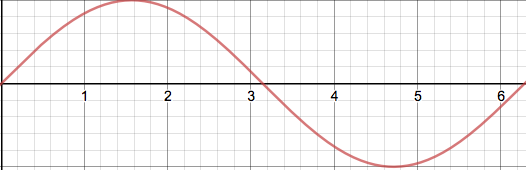
\includegraphics[width=1.75333in]{images/09_schroedinger/harmonic0.png}}
   \hspace{.2in}
  \subfloat{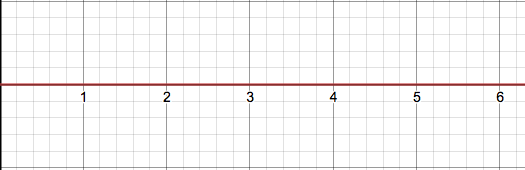
\includegraphics[width=1.75in]{images/09_schroedinger/harmonic1.png}}
   \hspace{.2in}
  \subfloat{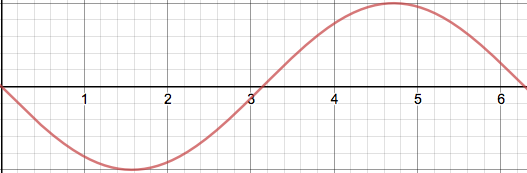
\includegraphics[width=1.75667in]{images/09_schroedinger/harmonic2.png}}
\end{figure}
The sinusoidal shape stays fixed in place, even as its amplitude diminishes to 0 and then passes 
over into the negative. But this is just what the separated form of the wave-function says: there 
is a shape, a function of the spatial coordinate, that does not vary with time, and a changing amplitude-factor that is the same throughout the whole spatial extent of the wave-function.

In the case of Schrödinger's wave equation (10), he considers a ``trial'' solution that is the product
of distinct spatial and temporal parts. We've already noted how this might facilitate finding a solution.
A futher simplification comes from the way the function of time is expressed, as a \emph{complex exponential}.

\vspace{5pt}
\emph{C. Complex Exponentials.} You will likely have encountered Euler's number, $e$, the base of the natural logarithm. And you may have encountered the imaginary unit $i = +\sqrt{-1}$, used in the definition of the \emph{complex numbers}, which have the form $a + bi$, where $a$ and $b$ are real numbers. Euler proved that, if it has any meaning at all, the expression $e^{i\theta}$ should be interpreted as equal to the complex number $\cos{\theta} + i\sin{\theta}$. If we imagine the complex numbers as represented in a plane, then the complex exponentials lie on the unit circle about the origin, and $\theta$ represents the arc length proceeding counter-clockwise around the circumference, starting from the point $1 + 0i$. 

Given the simplicity of the rules for differentiating and integrating the exponential, and the ease
with which it could be recast as a simple real-valued sinusoidal function (i.e.,
by ignoring the imaginary part), the complex exponential earned itself a place in the physicist's
mathematical toolbox. For our purposes, it is almost sufficient simply to know the rule
\begin{equation*}
de^{ix} = d(\cos{x} + i\sin{x}) = -\sin{x}\, dx + i\cos{x}\, dx = ie^{ix}\, dx.
\end{equation*}
Given this, it's easy to see that the factor $-4\pi^2\nu^2$ in (10') comes from differentiating the product
$\psi(x,y,z)e^{2\pi i\nu t}$ twice with respect to time, as does the similar factor in (12), after
the substitution of $E/h$ for the frequency $\nu$. Late in the next chapter, we will consider
more about how the complex form of the solution affects interpretation.

\vspace{5pt}
\emph{D. The Form of the Solutions.} In equation (11), Schrödinger points out what would be the
general solution if this were
simply the problem of finding the pressure waves in ``an elastic fluid in a given enclosure.''
There are a lot of terms, but if one imagines sinusoidal functions for each of the $\psi_k$, each
with its own amplitude $c_k$, and ignores the time-function and its frequencies and phase angles, 
it looks a lot like Bernoulli's 
formulation for the shape of the vibrating string. Bernoulli's component waves, of course, have
wavelengths that are submultiples of the length of the string, and in this way, his ``solution''
to the problem already includes the so-called ``boundary conditions,'' as does Schrödinger's
equation (11) in a general way (in its selection of frequencies $\nu_k$).

But by the time he gets to equation (14'), Schrödinger is referring to a far more definite set
of solutions. Along the way, he notes two ``complications'' and one ``simplification'' of the
wave equation for the electron in comparison with the fluid problem. One we noted above, the
dependency of the ``velocity'' term $u$ on the spatial coordinates, and the likeness between
this and the problem Euler imagined, of the string of varying thickness. But it's the simplification
that poses what could have been a ``fatal'' problem. In the case of Bernoulli's solution we just
mentioned (as well as in that of Euler's reformulation), the boundary conditions did some of the
work of selecting from among the infinite scope of possible solutions. Here, the electron could
be \emph{anywhere in space,} like one of de Broglie's ``pilot waves.''

In this first lecture to the Royal Institution introducing the very idea of wave mechanics to
a scientifically literate, but not necessarily expert, audience, Schrödinger is understandably
less than completely informative concerning ``the detailed process of finding the solutions,'' 
which would entail a ``rather lengthy mathematical discussion.'' Nonetheless, given the significant
work we have done both this year and last to understand wave phenomena and mechanics, we should
pause to fill in a little bit of the story here.

In somewhat naive terms, beginning from de Broglie, we might have imagined the wave threading
around the nucleus of the atom in one orbital plane, its crests and troughs aligning with one 
another. The functions that are unique solutions to Schrödinger's wave equation at a given energy level,
however, are rather more geometrically complicated. Schrödinger is a bit more forthcoming about
their form in the second lecture:

\begin{quote}
The detailed behavior of the ``elliptic'' functions within the said region [i.e., those belonging
to bound electrons, near the nucleus] cannot very well be described in a unique way, for the
following reason. To \emph{one} value of $E_n$ there belongs in general not only one, but 
precisely $n^2$ independent solutions of the wave equation. From the mathematical point of
view this is an exception due to the particular form of the potential energy $V$, especially to
its spherical symmetry[\ldots]. Since the equation is linear and homogeneous, any linear aggregate
with quite arbitrary coefficients [cf. equation (11)] will also be a solution belonging to the
\emph{same} proper value[\ldots]. To give an example: from a set of solutions whose node-surfaces
[i.e., surfaces with the same magnitude] are (1) concentric spheres, (2) co-axial cones, (3)
planes passing through the cone-axis, you can form other solutions, in which the concentric
spheres and co-axial cones are replaced by two sets of confocal paraboloids. This is only one
of the simplest cases. In general, taking arbitrary coefficients, the system of node-surfaces
will be \emph{much} more complicated.
\end{quote}

Two notes here: 1) the ``magnitude'' mentioned in the interpolation is the modulus squared
of the complex number that is the value of the wave-function: if the number is $a + bi,$
this is the non-negative real number $a^2 + b^2$; 2) the wave-function is in general spread
out in space, such that the node-surfaces formed by choosing a particular magnitude of the
function give only some of the information about the geometry of the function, as a
weather map might indicate gross features of the atmospheric pressure in a large region 
by tracing several lines of constant pressure (isobars). Perhaps you will have seen
representations of the higher-order ``orbitals'' in a book of chemistry. It is these 
shapes and details about the atomic behavior of electrons that Schrödinger's equations
allowed physicists to understand, even as the difficult work of interpreting the
physical meaning of the wave equation for a material particle was just beginning.
 

\chapter{Critique of the Physical Concepts of the Particle Picture}
\chapterprecis{Werner Heisenberg}

\makeoddhead{myheadings}{\emph{Heisenberg}}{}{\thepage}
\makeevenhead{myheadings}{\thepage}{}{\emph{Critique of the Physical Concepts of the Particle Picture}}

\renewcommand{\theequation}{\arabic{equation}}



\section*{The Physical Principles of the Quantum Theory\footnote{{[}\emph{Die
  Physikalischen Prinzipen der Quantentheorie}, Leipzig (1930); also
  \emph{The Physical Principles of the Quantum Theory}, trans. C. Eckart
  and F. C. Hoyt, Chicago (1930). The present selections were translated
  1995 by C. Burke and E. Brann, slightly revised in 2007 by H. Higuera
  and in 2014 by R. Druecker.{]}}\\
  {\large Werner Heisenberg}}

\subsection*{CHAPTER II\\
CRITIQUE OF THE PHYSICAL CONCEPTS OF THE PARTICLE PICTURE}

\subsubsection*{§I. The Indeterminacy Relations}

The concepts of position, velocity, and energy have been derived from
simple experiments of everyday experience, in which the mechanical
behavior of macroscopic bodies is described by these words. These
concepts were then carried over to electrons, since in some fundamental
experiments electrons show a mechanical behavior similar to objects of
everyday experience. But since we know that this similarity exists only
in a limited region, the range of applicability of the concepts of the
particle picture must be restricted in a corresponding way. According to
Bohr,\footnote{N. Bohr, \emph{Nature}, \textbf{121}, 580, 1928. {[}Note taken
  from English edition, giving citation to English version of Bohr's
  article.{]}} one arrives at this restriction in the simplest way by
recalling that all intuitable facts (i.e., facts describable in space
and time) of atomic physics must \emph{also} be describable in a wave
picture.

The following considerations apply equally to each of the three space
co-ordinates of the electron and are therefore carried out for only one.
The fact that the position of an electron is known with a certain
exactness $\Delta$\emph{x} {[}at the time \emph{t}{]} can obviously be
described in the wave picture by a wave function whose amplitude is
significantly different from zero only in a small range of approximate
magnitude $\Delta$\emph{x}. A wave function constructed in this way can always
be thought of as composed of a number of partial waves which interfere
with each other in such a way as to reinforce one another within the
small spatial range \emph{$\Delta$x} but cancel one another everywhere outside
that range. Such a configuration is called a \emph{wave packet}. A
general mathematical proposition states that it is always possible,
through appropriate composition of the individual partial waves, to
build up a wave packet of any desired shape. In the course of time such
a wave packet will in general change its size and shape and, apart from
special cases, will ultimately be dispersed over the whole of space. The
velocity of the electron likewise corresponds to the velocity of the
wave packet; however, no exact velocity can be defined for the wave
packet because, as was said, besides its forward motion, it also spreads
and disperses itself. This dispersion thus occasions an indeterminacy in
the definition of the momentum (mass times velocity) of the amount, say,
$\Delta$\emph{p}. Now, from the simplest laws of optics, together with the
equations
\begin{equation*}
{[}\lambda = \frac{h}{p} \quad\quad \text{and} \quad\quad v_g = \frac{h}{\mu\lambda_0}{]}
\footnote{{[}Heisenberg derives these equations in an
  appendix and references them here rather than writing them out. For
  further details see footnote 6 below.{]}}
\end{equation*}
it can be derived that
\begin{equation}
\Delta x\Delta p_x \geq h. % eqn (1)
\end{equation}

For, think of the wave packet as being composed out of the superposition
of plane {[}sinusoidal{]} waves, whose wave-lengths are to lie in the
neighborhood of $\lambda_0$. Then, on the whole,
$n = \Delta x/\lambda_0$ crests or troughs fall in the region
inside the packet. Outside the packet the plane waves are to cancel each
other by interference; this is possible if, and only if, the totality of
component plane waves contains some for which at least $n + 1$
waves fall in the critical range. This gives
\begin{equation*}
\frac{\Delta x}{\lambda_0 - \Delta\lambda} \geq n + 1 ,
\footnote{{[}The waves of
  longer and shorter wavelength must reinforce each other at the center
  of the packet and interfere at each end. Hence they must be out of
  coincidence by one-half wavelength at each end, which is only possible
  if the shorter waves are contained at least one more time than are the
  longer waves in the same distance $\Delta$\emph{x}. If there are
  $n=\Delta x/\lambda_0$ of the longer waves of length $\lambda_0$ in the
  packet, then there must be at least $n + 1$ of the shorter waves
  of length $\lambda_0 - \Delta\lambda$ within the same region $\Delta x$.{]}}
\end{equation*}
where $\Delta\lambda$ indicates approximately the range of wave-lengths which
is necessary for the representation of the packet. Consequently
\begin{equation}  % eqn (2)
\frac{\Delta x\Delta\lambda}{\lambda^2_0} \geq 1 .\footnote{{[}From the 
  inequality at the end of the previous note,
  \begin{equation*}
  \frac{\Delta x}{\lambda_0-\Delta\lambda} \geq n + 1 = \frac{\Delta x}{\lambda_0} + 1,
  \end{equation*}
  collecting algebraic terms to the left and adding gives,
  \begin{equation*}
  \frac{\Delta x\Delta\lambda}{\lambda_0(\lambda_0-\Delta\lambda)} \geq 1 ,
  \end{equation*}
  which can be approximated to inequality (2) if $\Delta\lambda$ is
  sufficiently small compared to $\lambda_0$.{]}}
\end{equation}
On the other hand, the group velocity of the waves is
\begin{equation}
v_g = \frac{h}{\mu\lambda_0} .  % eqn (3)
\footnote{{[}As just mentioned, Heisenberg derives equation (3) in an
  appendix. Here $\mu$ is the mass of an electron. Now if in de
  Broglie's $\lambda = h/p (=h/\mu v)$ one stipulates that the de
  Broglie wavelength of the \emph{electron} is ``the''
  $\lambda_0$ of the \emph{packet} and that the velocity
  of the electron equals the group velocity, one gets $\lambda_0=h/\mu v_g$, from
  which eq. (3) follows immediately. But Heisenberg actually derives eq.
  (3) \emph{directly from the Schrödinger wave equation} and,
  without relying on ``particle'' concepts. As he writes, ``The wave
  theory does not consider electrons, {[}but{]} merely universal
  constants of the wave equation.''{]}}
\end{equation}
The dispersion of the packet corresponding to the range $\Delta\lambda$ is
therefore characterized by {[}a range of velocities{]}
\begin{equation*}
\Delta v_g \approx \frac{h}{\mu\lambda_0^2}\Delta\lambda .
\footnote{{[}If one does \emph{not} impose assumptions from the
  particle picture, then in the packet \emph{both} the longer \emph{and}
  the shorter waves have an equal claim to be considered ``the''
  wavelength for purposes of equation (3). That equation is already
  written for the longer wavelength $\lambda_0$. Were it instead to be
  written for the shorter wavelength, $\lambda_0 - \Delta\lambda$, there would
  be determined a different group velocity,
  \begin{equation*}
  v'_g = \frac{h}{\mu(\lambda_0-\Delta\lambda)}
  \end{equation*}
  and the difference between $v'_g$ and $v_g$ is the ``range of
  velocities'' $\Delta v_g$. Thus
  \begin{equation*}
  \Delta v_g =\frac{h}{\mu(\lambda_0-\Delta\lambda)}-\frac{h}{\mu\lambda_0} =
  \frac{h\Delta\lambda}{\mu\lambda_0(\lambda_0-\Delta\lambda)}\approx\frac{h\Delta\lambda}{\mu\lambda^2_0}
  .{]}
  \end{equation*}
}
\end{equation*}
  By definition $\Delta p_x = \mu\Delta v_g$, and therefore by
  equation (2),
\begin{equation*}
  \Delta x\Delta p_x \geq h
  . \footnote{{[}Substituting from the
  equation for $\Delta v_g$, $\mu\Delta v_g = \mu\frac{h}{\mu\lambda_0^2}\Delta\lambda
  = h\frac{\Delta\lambda}{\lambda^2_0}$. Therefore, $\Delta x\Delta p_x = h\frac{\Delta x\Delta\lambda}{\lambda^2_0}$; 
  that is, by equation (2), $\Delta x\Delta p_x$ equals $h$ times something $\geq 1$.{]}}
\end{equation*}\\
\centerline{* * *}
%
The indeterminacy relations [\ldots] specify the limits within which the
concepts of the particle theory can be applied. Any use of the words
``position'' or ``velocity'' with an exactness exceeding that indicated
by equation (1) is just as empty of content as the use of words whose
sense has not been defined.\footnote{In this connection one should
  particularly remember that the human language quite generally permits
  the construction of sentences from which no consequences follow and
  which are therefore completely empty of content, although these
  sentences produce a kind of intuitable representation. For example,
  the assertion that besides our world there exists another world, with
  which any connection is impossible \emph{in principle}, does not lead
  to any inference; nevertheless, accompanying this statement a kind of
  picture arises in the imagination. Obviously such a statement can
  neither be proved nor disproved---one should be especially careful in
  the use of the expression ``in actuality'' since it very often leads
  to assertions of the type just discussed.}\\
\centerline{* * *}
%
\subsubsection*{§2. Confirmation of the Intedeterminacy Relations using Various
Measuring Devices}

The indeterminacy relations relate to the degree of exactness in our
present (simultaneous) knowledge of the various quantum-theoretical
magnitudes. Since these relations do not restrict the exactness, for
example, of a position measurement alone or a velocity measurement
alone, their effect expresses itself only in the fact that each
experiment that makes possible a measurement of, say, position,
necessarily disturbs the knowledge of the velocity to a certain degree.
Let us suppose, for example, that the velocity of a {[}free{]} electron
is exactly known, while the position is completely unknown. Then every
subsequent observation of the position must alter the momentum of the
electron, and this alteration must be indeterminate by an amount such
that after the experiment is carried out our knowledge of the electron's
motion is limited by the indeterminacy relations. This will be confirmed
in what follows, using some experiments as examples. But first let it be
remarked that the indeterminacy relations evidently do not refer to the
past. For if the velocity of the electron is known to begin with, and
subsequently the position is exactly measured, then the electron's
positions for the time \emph{before} the measurement of position may
also be exactly calculated. For this previous time, the quantity
$\Delta p\Delta x$ will be smaller than the usual limiting value. This
knowledge of the past, however, is of a purely speculative character,
since---because of the change in momentum caused by the position
measurement---it can in no way enter as an initial condition in any
calculation concerning the future of the electron, and never makes an
appearance in any physical experiment at all. It is thus a pure matter
of taste whether or not one is to ascribe to such a calculation
concerning the past of the electron any physical reality.

\begin{figure}[h] % Figure 5
  \begin{center}
    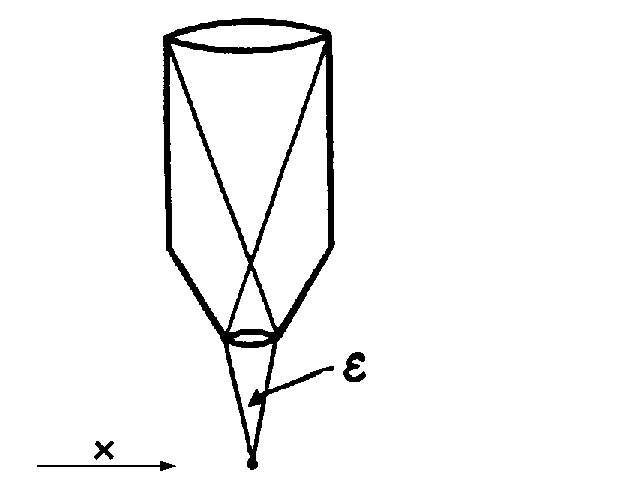
\includegraphics[width=1.875in,height=1.40625in]{images/10_heisenberg/image015.png}
  \end{center}
  \caption*{\emph{Figure 5.}\footnote{{[}The figure is that of the 1930 Chicago edition and
  corrects an error in the Leipzig edition.{]}}}
\end{figure}
%\includegraphics[width=1.875in,height=1.40625in]{media/image18.png}

a) \emph{Determination of the position of a free particle.}---As a first
example of the disturbance of the knowledge of a particle's momentum by an
apparatus for measuring position, we choose the position measurement by
means of a microscope.\footnote{N. Bohr, \emph{loc. cit.}} Let the
electron be moving at such a distance under the objective of the
microscope that the cone of rays scattered from it has an angular
opening $\varepsilon$. Let the wave-length and frequency of the light
illuminating the electron be $\lambda$ and $\nu$; then the exactness
in the position measurement of the $x$-direction (see Fig.\ 5)
according to the {[}limit on resolving power of any optical
instrument{]} is:\footnote{{[}The resolving power of a lens is limited
  by the aperture of the lens, since any small opening will diffract any
  light it transmits. If the central maxima of the diffraction patterns
  of two objects then overlap to any great extent, those objects will be
  indistinguishable through the lens. The separation, $\Delta x$, at
  which two ``point'' objects can no longer be distinguished sets a
  limit to our ability to determine the position of an object with a
  microscope---a limit which depends on the angular aperture of the
  objective lens and the wavelength of the illuminating light. A
  derivation of equation (16) is given in the Note at the end of this chapter.{]}}
%
\begin{equation*}\tag{16}
\Delta x \approx \frac{\lambda}{\sin \varepsilon} .
\end{equation*}
%
But for a position measurement to be possible, at least one photon must
be scattered from the electron and pass through the microscope to reach
the eye of the observer. From this one photon, the electron receives a
Compton recoil\footnote{{[}Recall that the interaction of light
  with electrons can be understood as an \emph{elastic collision}
  between electrons and photons if the photons of energy
  $e= h\nu$ are also assigned momentum of amount $p = h/\lambda$.

  In the sketch, a photon after rebounding from a particle will have
  momentum $h/\lambda$. If it enters the microscope it must fall
  within the angle $\varepsilon$ and therefore will carry away momentum
  $px$ in the $x$-direction, which can be as little as
  \emph{zero} or as much as $(h/\lambda)\sin \varepsilon$. But since the
  direction of any particular photon cannot be distinguished by the
  microscope, the momentum of the particle is unknown within a range
  equal to $(h/\lambda)\sin \varepsilon$.{]}
  \begin{center}
    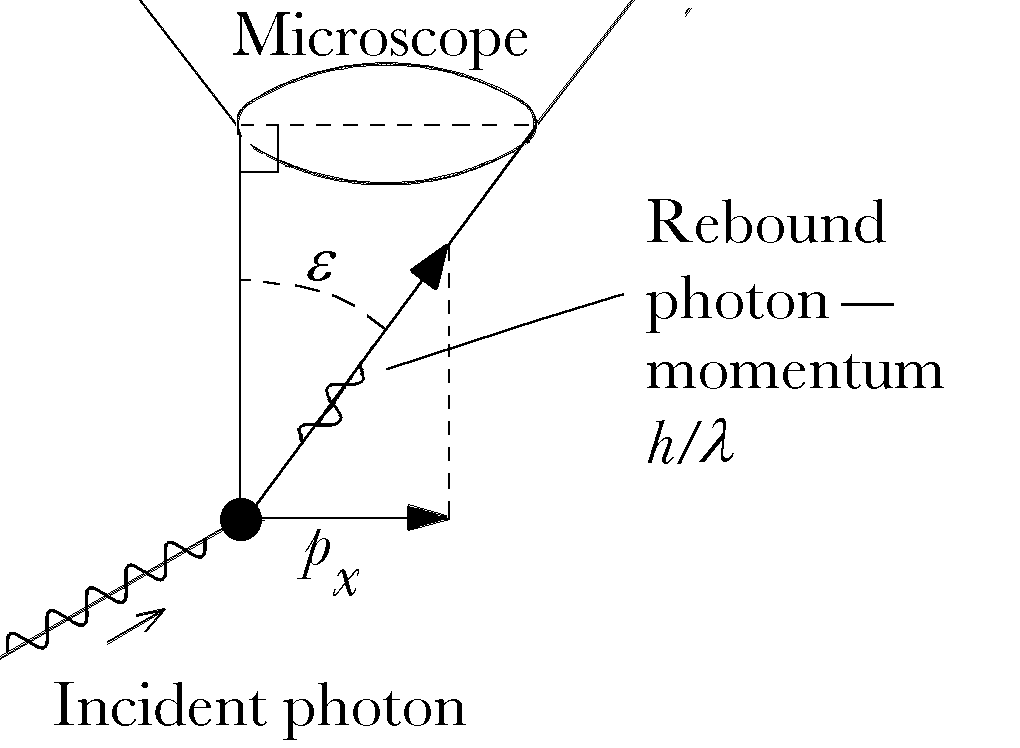
\includegraphics[width=1.7in,height=1.24667in]{images/10_heisenberg/image054.png}
  \end{center}
  } of order of magnitude
$h/\lambda$. The recoil cannot be known exactly, since within the bundle
of rays (of angular opening $\varepsilon$) the direction of the photon
{[}entering the microscope{]} is unknown.\footnote{{[}There is a lens
  across the aperture. If the microscope is focused properly, then
  according to ray-optics \emph{wherever} the ``ray'' of light passes
  through the lens, it will be refracted onto the same point on the
  detecting screen.{]}} Thus there will be an uncertainty of the recoil
in the $x$-direction of amount
%
\begin{equation*}\tag{17}
\Delta p_x \sim \frac{h}{\lambda}\sin \varepsilon % eqn (17)
\end{equation*}
%
and it follows for the knowledge of the electron's motion after the
experiment that
%
\begin{equation*}\tag{18}
\Delta x\Delta p_x \sim h. % eqn (18)
\end{equation*}
%

Objections may at first be raised against this derivation: The reason
for the indeterminacy of the recoil is, after all, that it is unknown
which path within the bundle of rays the photon takes. One might thus
try to determine this path by making the whole microscope movable and
measuring the recoil that it receives from the photon. But this will not
help to circumvent the indeterminacy relations; for there then
immediately arises the question of the position of the microscope, and
the position and momentum of the whole microscope will also be subject
to equation (18). To be sure, the measurement of the position of the
microscope could be neglected altogether if the electron and a fixed
scale could be simultaneously observed through the movable microscope.
But then one observation would require the simultaneous passage of at
least two photons through the microscope to the observer---one from the
scale and one from the electron---and a measurement of the recoil of the
microscope would no longer yield information about the photon coming
from the electron, and so on.

The whole discussion of this experiment characteristically makes use of
the wave picture and the particle picture simultaneously. Here we make
use of that duality essentially in the theory of radiation; for on the
one hand we speak of bundles of rays and the laws of optics, and on the
other hand, of photons and the recoils caused by them.

%
\begin{figure}[h] % Figure 6
  \begin{center}
    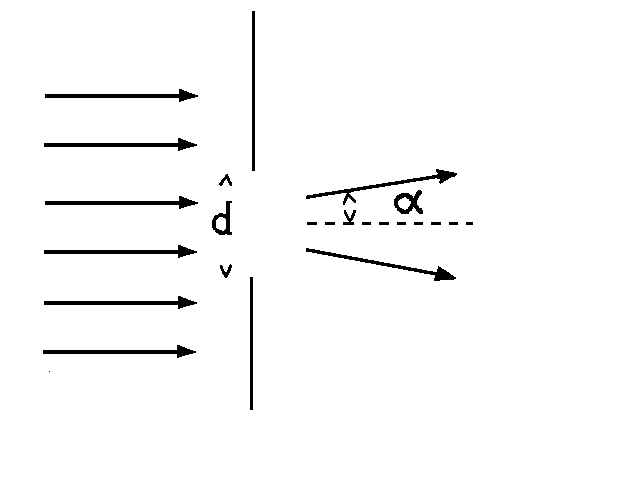
\includegraphics[width=1.875in,height=1.4414in]{images/10_heisenberg/image021.png}
  \end{center}
  \caption*{\emph{Figure 6.}\footnotemark}
\end{figure}
\footnotetext{[The figure is that of the 1930 Chicago edition and
  corrects an error in the Leipzig edition.]}
%

Another simple determination of position can be performed in the
following way: Again let the velocity of the electron be completely
known. Consider a set of possible paths which an electron might take in
approaching a screen that contains a slit of
width $d$ (Fig. 6). If the electron passes through this slit, then evidently
its position in the direction parallel to the screen is fixed with
exactness $\Delta x = d$. If the oncoming electron is represented
by a plane de Broglie wave, however, one sees immediately that
diffraction will occur. The emerging wave will have a finite angular
opening $\alpha$ which, by the simplest laws of optics,\footnote{{[}``The
  simplest laws of optics:'' Heisenberg refers to the expression for
  single-slit diffraction, $\sin \theta_1 = \lambda/d$,
  where $\theta_1$ is the half-width of the central maximum (see the Note
  at the end of this chapter).{]}} will be given by
%
\begin{equation*}\tag{19}
\sin \alpha \sim \frac{\lambda}{d} , % eqn (19)
\end{equation*}
%
where \emph{$\lambda$} is the wave-length of the de Broglie waves. Thus the
momentum of the electron parallel to the screen, after the electron's
passing through the slit, is uncertain by an amount
%
\begin{equation*}\tag{20}
\Delta p_x = \frac{h}{\lambda}\sin \alpha % eqn (20)
\end{equation*}
%
since $h/\lambda$ is the momentum of the electron in the direction of the
beam. Then, since $\Delta x = d$, it follows that
%
\begin{equation*}
\Delta x \Delta p_x \sim h.
\end{equation*}
%
In this derivation, although no use is made of the wave-particle duality
in the theory of radiation, it is indeed used in the theory of matter.\\
\centerline{* * *}
%
\subsection*{CHAPTER IV\\ 
THE STATISTICAL INTERPRETATION OF QUANTUM THEORY\footnote{{[}\emph{Nature}, 121,
  580, 1928. Again, citing the English version.{]}}}
\centerline{* * *}

\subsubsection*{§3. Bohr's Concept of Complementarity}


The world of concepts derived from everyday experience was for the first
time left behind in Einstein's relativity theory. It became apparent
that the ordinary concepts could only be applied to processes in which
the velocity of the propagation of light could be regarded as
practically infinite. The experiential material which has been refined
through modern experimental physics thus necessitated the revision of
received concepts and the development of new ones; but our thinking
could adjust itself only slowly to that extended range of experience and
the world of its concepts; and therefore relativity theory itself
seemed at first abstract and alien. As is clear from what has been said,
the experiences from the world of atoms compel us to an even more
extensive renunciation of hitherto customary concepts. Indeed, our
ordinary description of nature and especially the thought of a strict
lawfulness in the processes of nature rest on the assumption that it is
possible to observe phenomena without appreciably influencing them. To
co-ordinate a determinate cause to a determinate effect has a meaning
only when we can observe effect and cause without simultaneously
disturbing the process by our intervention. The law of causality in its
classical form can thus, by its nature, be defined only for isolated
systems. But in atomic physics there is in general connected with each
observation a finite disturbance that is to a certain degree
uncontrollable, as was from the very beginning only to be expected in
the physics of what are in principle the smallest units. Since, on the
other hand, every space-time description of a physical process is
conditioned by the observation of the process, it follows that the
space-time description of processes on the one hand, and the classical
law of causality on the other, represent complementary and mutually
exclusive features of the physical event. What corresponds to this
situation in the formalism of the theory is the fact that while a
mathematical model of quantum theory exists, this model cannot be
interpreted as a simple connection of things in space and time. Through
this complementarity of the space-time description on the one hand, and
of the causal connection on the other, there arises moreover a peculiar
ambiguity in the concept ``observation'' in that it is left arbitrary
which objects are to be counted as belonging to the observed system and
which are to be regarded as means of observation. In the formalism of
the theory this arbitrariness has the consequence that often quite
heterogeneous methods can be used for the interpretation of a physical
experiment [\ldots]. But even if one accepts the arbitrariness mentioned,
the concept ``observation'' belongs strictly speaking to the world of
ideas drawn from our everyday experience. It can be carried over to
atomic phenomena only when due regard is paid to the limitation placed
on all space-time pictures by the indeterminacy relations. For every
observation is by definition bound to space and time; therefore, this
concept has meaning only within the boundaries specified by those
relations. It has already been mentioned that there are special cases in
which the requirements of the classical law of causality can be brought
into agreement with a spatio-temporal description to a certain
approximation. In general, however, the situation can be characterized
by something like the following diagram:

\begin{figure}[h] % Figure 5
  \begin{center}
    \includegraphics[width=5.1in,height=2.08in]{images/10_heisenberg/heisenberg-table.png}
  \end{center}
\end{figure}

It is only after attempting to adjust the formation of one's concepts
to this fundamental complementarity of space-time description and
causality, that one is in a position to judge whether the methods of
quantum theory are free of inconsistency [\ldots]. The adaptation of our
thought and our language to the experiences of atomic physics is indeed
associated with great difficulties, just as it had been for relativity
theory. In relativity theory the earlier philosophical discussions of
the problems of space and time proved to be very serviceable to this
adaptation. In a similar way one can profit in atomic theory from the
discussions, fundamental to all epistemology, concerning the
difficulties connected with the separation of the world into subject and
object. Quite a few abstractions which are characteristic of modern
theoretical physics will be found to have been already discussed in the
philosophy of past centuries. While these abstractions could in the past
be rejected as thought-play by the natural scientist intent only on
realities, the more refined experimental art of modern physics now
forces us to discuss them thoroughly.\\
\centerline{* * *}
%

\section*{M. BORN: THE PROBABILITY INTERPRETATION}

Physicists generally came to accept the mathematical formalism of the
$\Psi$ waves as initiated by de Broglie and developed by Schrödinger.
However, there was a lively debate over the \emph{interpretation} of
them. Einstein, for example, as we shall see later on, thought that, in
some sense, the $\Psi$ function did not give the complete account of
entities like electrons because it was based upon inadequate concepts of
classical physics.

Aside from this suggestion there seem to be, roughly speaking, three
possibilities. As was seen in Chapter \ref{ChDeB}, de Broglie thought of an
electron as simultaneously \emph{both} a particle \emph{and} a wave.
Secondly, one might hold that an electron is \emph{only} a wave, and not
a particle at all. De Broglie's second presentation of his idea of wave
mechanics suggests the following reasoning: Huygens and Young saw that
if wave optics is correct, there really are no light particles but only
light waves that appear as straight-line particle paths due to the
smallness of the wavelength in comparison with the size of the objects
with which the waves interact. So too it should be the case that if wave
mechanics is correct, there really are no material particles but only
$\Psi$ waves that appear as particles in certain situations. This is
the approach taken by Schrödinger. He considered that a particle was
simply a wave packet, and he associated the function $\Psi$ in a
certain way with the density of charge in space.

The third approach, the so-called ``Copenhagen interpretation,''
according to which an electron is \emph{either} a particle \emph{or} a
wave---in the sense that it exhibits now particle-like behavior, now
wave-like behavior---but never both simultaneously, was the one
developed by Bohr and Heisenberg.

The Copenhagen complementarity interpretation of the electron was joined
with an interpretation of the wave function $\Psi$ proposed by Max
Born. According to this interpretation, the wave function at any point
in space, $\Psi(x,y,z,t)$, is to be viewed as determining a
\emph{probability density}---that is, the probability, per unit volume,
of \emph{observing}\footnote{``Observing'' includes, for example, having
  a particle cause a glow on a screen at a point.} \emph{a particle}
very near that point.

In the following passage from his textbook,\footnote{\emph{Atomic
  Physics} (New York: Hafner, 1962), 96-100.} Born begins the
presentation of his interpretation by opposing that of Schrödinger:

\begin{quotation}
In the preceding sections we have had a series of facts brought before
us which seem to indicate unequivocally that not only light, but also
electrons and matter, behave in some cases like a wave process, in other
cases like pure corpuscles. How are these contradictory aspects to be
reconciled?

To begin with, Schrödinger attempted to interpret corpuscles, and
particularly electrons, as \emph{wave packets.} Al­though his formulae
are entirely correct, his interpretation cannot be main­tained, since on
the one hand, as we have already explained above, the wave packets must
in course of time become dissipated {[}see below{]}, and on the other
hand the description of the interaction of two electrons as a collision
of two wave packets in ordinary three‑dimensional space lands us in
grave difficulties.\footnote{{[}Born's second reason against the
  possibility of maintaining Schrödinger's interpretation is the
  following: The extension of Schrödinger's theory to an interaction
  between two particles involved six spatial coordinates, three for each
  particle. Thus, on the most natural generalization of Schrödinger's
  theory, the $\Psi$ waves became waves in a non-physical,
  six-dimensional space, a consequence which does not accord with the
  interpretation of the $\Psi$ waves as representing physical waves.
  And attempts to treat a two-particle situation in a different way so
  as to preserve the physical character of the $\Psi$ wave had not
  born fruit.{]}}

The interpretation generally accepted at present goes back to the
present writer. According to this view, the whole course of events is
determined by the laws of probability; to a state in space there
corresponds a definite probability, which is given by the de Broglie
wave associated with the state. A mechanical process is therefore
accompanied by a wave process, the guiding wave, described by
Schrödinger's equation, the significance of which is that it gives the
probability of a definite course of the me­chanical process. If, for
example, the amplitude of the guiding wave is zero at a certain point in
space, this means that the probability of finding the electron at this
point is vanishingly small.

The physical justification for this hypothesis is derived from the
con­sideration of scattering processes from the two points of view, the
cor­pus\-cular and the undulatory. The problem of the scattering of light
by small particles of dust or by molecules, from the standpoint of the
classical wave theory, was worked out long ago. If the idea of light
quanta is to be applied, we see at once that the number of incident
light quanta must be put proportional to the intensity of the light at
the place concerned, as calculated by the wave theory. This suggests
that we should attempt to calculate the scattering of electrons by
atoms, by means of wave mechanics. We think of an incident beam of
electrons as having a de Broglie wave associated with it. When it passes
over the atom this wave generates a secondary spherical wave; and
analogy with optics sug­gests that a certain quadratic expression formed
from the wave {[}function $\Psi${]} should be interpreted as the
current strength, or as the number of scat­tered electrons.\footnote{{[}See Chapter \ref{ChDeB}, note \ref{noteDeBroglie}, p.~\pageref{noteDeBroglie}.
  We know that \emph{p $\propto$ N $\propto$ I $\propto$ F\textsuperscript{2}}.
  Analogously, for the matter wave function \emph{$\Psi$(x,y,z,t),} the
  probability of finding the particle in a certain region, Born proposed,
  would be the integral of the modulus squared of
  the wave-function over that region. Though the value of the wave-function
  is complex, its modulus squared is always real and non-negative. If
  the wave-function is ``normalized,'' such that its magnitude over all
  space is set equal to 1, then the probability of finding its particle
  in a given region will always be $\leq 1$.{]}} On carrying out the calculation it
has been found that for scattering by a nucleus we get exactly
Rutherford's formula. Many other scattering processes were afterwards
subjected to calculation in this way, and the results found in good
agreement with observation. These are the grounds for the conviction of
the correctness of the principle of associating wave {[}function{]} with
number of particles (or probability). . . .

What, then, is a problem with physical meaning? This is for us the
really important question, for clearly enough the corpuscular and wave
ideas cannot be fitted together in a homogeneous theoretical formalism,
without giving up some funda­mental principles of the classical theory.
The unifying concept is that of probability; this is here much more
closely interwoven with physical principles than in the older physics.
\end{quotation}

The following passage\footnote{H. Boorse and L. Motz, edd., \emph{The
  World of the Atom}, Vol. II, 1079.} presents an analogy as an aid
to understanding Born's hypothesis:

\begin{quotation}
Born assumed that the De Broglie wave associated with a scattered beam
of electrons would be a measure of the probability for that particular
state of scattering. In general, therefore, the square of the amplitude
of the De Broglie wave of an electron determines the probability of
find­ing the electron in a given region of space.

We may illustrate this point by drawing an analogy between the De
Broglie waves of a collection of particles and the water waves on the
ocean. If we watch the ocean, we observe that the surface is in constant
agitation. The disturbances range from small ripples to large waves. The
greater the amplitude of a wave, that is, the higher above the surface
of the ocean is the crest of the wave, the more intense is the
disturbance of the water at that point. Where there is no disturbance at
all, the water is perfectly smooth and the amplitude of the wave is
zero. We now picture the space surrounding an electron or a swarm of
electrons as being similar to the surface of the ocean. But the waves
with which we are now con­cerned are not physical ones, but rather
probability waves, or waves that are a measure of the probability for
finding the electron, or groups of electrons, at particular points in
space. The greater the intensity of a De Broglie wave at a point, the
greater is the probability for finding the electron there; should the
amplitude of the De Broglie wave vanish at any point, the probability
for finding the electron there is zero.

Suppose we consider an electron in a region of space in which the De
Broglie wave is spread out uniformly, so that the amplitude of the wave
is everywhere the same. This means that there is an equal probability of
finding the electron at any point in this region. What happens, then, if
we perform an experiment in which we look for the electron and locate it
at a given point in this region? For example, we can place a fluorescent
screen in some position and if the electron happens to strike it, we
observe a scintillation at the point where it hits the screen. Since we
know that the electron is precisely at this point of scintillation on
the screen, the proba­bility of finding the electron there is one and
the probability of finding the electron elsewhere at this time is zero.
This means that we may think of the De Broglie wave describing the
electron, which originally was spread out uniformly, as now concentrated
in a tiny packet. Thus, by perform­ing an experiment we have altered the
nature of the wave describing the electron and therefore the future
unfolding of the probability.
\end{quotation}

This interpretation appealed to Born for the additional reason that it
brings particles into close analogy with light. As we saw, de Broglie
and Einstein linked the Maxwellian wave with the photon by making the
square of the amplitude of (the electric component of) that wave at any
point give the probability that a photon will interact with an atom or
electron there. Adopting an analogous interpretation for $\Psi$ made
particles and light that much more similar mathematically and, it was
hoped, would help in understanding whatever real kinship they must have.

While Born's probability interpretation of $\Psi$ became an essential
part of the orthodox Copenhagen interpretation, Schrödinger, Einstein
and, after 1952, de Broglie dissented. Schrödinger, for example, wrote
in 1953\footnote{{[}``What Is Matter?'' \emph{Scientific American}
  (September, 1953), 56.{]}}:

\begin{quote}
The wave v. corpuscle dilemma is supposed to be resolved by asserting
that the wave field merely serves for the computation of the probability
of finding a particle of given properties at a given position if one
looks for it there. But once one deprives the waves of reality and
assigns them only a kind of informative role, it becomes very difficult
to understand the phenomena of interference and diffraction on the basis
of the combined action of discrete single particles. It certainly seems
easier to explain particle tracks in terms of waves than to explain the
wave phenomenon in terms of corpuscles.
\end{quote}

Thus, when Heisenberg speaks of a ``probability function'' in the
discussion that follows, he is referring to $\Psi$.


\section*{The Copenhagen Interpretation of Quantum Theory\footnote{[From Chapter
  III of \emph{Physik und Philosopie}, Stuttgart (1959); also
  \emph{Physics and Philosophy: The Revolution in Modern Science}
  (1962). The present selection was translated 1995 by C. Burke and E.
  Brann.]}\\
  {\large Werner Heisenberg}}


The Copenhagen interpretation of quantum theory begins with a paradox.
Every physical experiment, it matters not whether it refers to a
phenomenon of daily life or to atomic physics, must be described through
the concepts of classical physics. These classical concepts form the
language by which we indicate the arrangement of our experiments and
determine the results; and we cannot replace them by any others.
Nevertheless the application of these concepts is limited by the
relations of indeterminacy. We must keep in mind this limited range of
applicability of the classical concepts while using them, but we cannot
and should not try to improve them.

For a better understanding of this paradox it is useful to see how the
interpretation of an experiment in classical physics differs from that
of an experiment in quantum theory. In Newton's celestial mechanics, for
instance, we may start by measuring the position and the velocity of the
planet whose motion we are going to study. The results of the
observation are translated into mathematics by deriving numbers for the
co-ordinates and the momenta of the planet from the observation. Then
the equation of motion is used to determine from these values of the
co-ordinates and momenta at a given time the values of these
co-ordinates or any other properties of the system at a later time, and
in this way the astronomer can predict the properties of the system at a
later time. He can, for instance, predict the exact time for an eclipse
of the moon.

In quantum theory the procedure is somewhat different. We might, for
instance, be interested in the motion of an electron in a cloud chamber
and could determine by some kind of observation the initial position and
velocity of the electron. But this determination will not be exact. It
will at least contain the inexactnesses {[}\emph{die Ungenauigkeiten}{]}
which follow necessarily from the indeterminacy relations and will
probably contain besides, still very much greater inexactnesses which
are conditioned by the difficulties of the experiment. The first of
these inexactnesses gives us the possibility of translating the result
of the observation into the mathematical formalism of quantum theory. A
probability function is written down which represents the experimental
situation at the time of the measurement, including the possible
inexactness of the measurement.

This probability function represents a mixture of two different
elements, {[}on the one hand{]} a fact and {[}on the other hand{]} the
degree of our knowledge of a fact. It represents a fact in so far as it
assigns to the initial situation a probability of 1, that is, complete
certainty. It is completely certain that the electron has moved with the
observed velocity at the observed position. ``Observed'' does mean, to
be sure, observed within the exactitude of the experiment. It represents
the degree of our knowledge insofar as another observer might perhaps
have known the position of the electron even more exactly. The
experimental error or the inexactness of the experiment can, at least to
a certain degree, be regarded as not a property of the electron but as a
deficiency in our knowledge of the electron. This deficiency in
knowledge, too, is expressed through the probability function.

In classical physics, too, careful observation must take observational
errors into consideration. The result one then gets is a probability
distribution for the initial values of the co-ordinates and velocities
and therefore something similar to the probability function of quantum
mechanics. But the special uncertainty which necessarily follows from
the indeterminacy relations is missing in classical physics.

As soon as the probability function in quantum theory has been
determined for the initial time from the observation, one can calculate
the function at any later time from the laws of quantum theory and can
thereby determine beforehand the probability that a measurement will
yield a certain value for the magnitude to be measured. We can, for
instance, predict the probability of finding the electron at a later
time at a certain point in the cloud chamber. It should be emphasized,
however, that the probability function does not in itself represent a
course of events in time. It represents something like a tendency for
events {[}\emph{Vorgänge}{]}, the possibility of events or our knowledge
of them. The probability function can be connected with actuality
{[}\emph{Wirklichkeit}{]} only when one essential condition is
fulfilled: when a new measurement or observation is made to determine a
certain property of the system. Only then does the probability function
allow us to calculate the probable result of the new measurement. The
result of the measurement will in this case again be stated in terms of
classical physics. . . .

It has already been said that the atom consists of a nucleus and of
electrons moving around the nucleus. It has also been stated that the
concept of an electronic orbit is somewhat doubtful. Against the latter
formulation a first objection might be that it should be possible at
least in principle to observe the electron in its orbit. . . .
{[}However{]} one can easily see that it is evidently not possible to
observe the orbit of the electron around the nucleus. {[}The development
of the probability function in time{]} shows not a wave packet that
moves around the nucleus, but one that moves away from the nucleus,
since the first photon {[}to strike the electron{]}\footnote{{[}Heisenberg
  refers to an earlier discussion of the possibility of observing the
  electron through a hypothetical microscope which uses high energy
  $\gamma$-rays, whose wave-length is smaller than the size of the
  atom.{]}} will already have knocked the electron out of the atom. This
is so because the momentum of the $\gamma$-ray quantum must be
considerably larger than the original momentum of the electron if the
wavelength of the $\gamma$-ray is much smaller than the size of the
atom. Therefore, the first photon is already sufficient to knock the
electron out of the atom, and one can never observe more than one point
in the orbit of the electron. Hence one does not fall into a
contradiction with experience if one asserts that there are, in fact, no
electron-orbits in the ordinary sense.

The next observation . . . will thus show the electron on its path away
from the atom. In the most general sense it is impossible to describe
intuitively what happens between two consecutive observations. It is of
course tempting to say that the electron must have been somewhere during
the time between the two observations and that therefore it must have
described some kind of orbit or path, even if it should be impossible to
establish this path. This would be a reasonable argument in classical
physics. But in quantum theory it would be case of a misuse of language
which, as we will see later, cannot be justified. We may leave it open
for the moment, whether this warning is an assertion about the way in
which we should speak about atomic events or an assertion about the
events themselves---whether it is a matter, as it were, of epistemology
or of ontology. In any case, we have to use the most extreme caution
about the formulation of any assertion which concerns the behavior of
atomic particles.\footnote{{[}In \emph{The Physical Principles of the
  Quantum Theory} {[}33--34{]}, Heisenberg adds the following about
  atomic orbitals: ``{[}For any energy level{]} there is . . . always a
  small but finite probability of finding the {[}``bound''{]} electron
  at a great distance from the center of the atom. {[}At that
  distance{]} the potential energy {[}is almost zero{]}. The kinetic
  energy is always positive; so that the total energy is therefore
  certainly greater than the energy of the stationary state under
  consideration {[}which must be negative, and quite sizably so for
  lower energy-levels{]}. This paradox finds its resolution when the
  energy imparted to the electron by the photon used in making the
  position measurement is taken into account. This energy is
  considerably greater than the ionization energy of the electron, and
  thus suffices to prevent any violation of the law of conservation of
  energy.''{]}}

Actually we need not speak of particles at all. For many experiments it
is more convenient to speak of \emph{matter waves}; for instance, of
standing oscillations of the electron-matter about the atomic nucleus.
Such a description would, to be sure, directly contradict the other
description if one did not pay attention to the limits set by the
indeterminacy relations. Through these limitations the contradiction is
avoided. The use of the concept of matter waves is convenient, for
example, when dealing with the radiation emitted by the atom. By means
of its frequency and intensity the radiation gives information about the
oscillating charge distribution in the atom, and there the wave picture
comes much nearer to the truth than the particle representation. Bohr
therefore advocated the use of both pictures, which he called
``complementary'' to each other. The two pictures are of course mutually
exclusive, because a certain thing cannot at the same time be a particle
(that is, a substance confined to a very small volume) and a wave (that
is, a field spread out over a large space); but the two pictures
complete each other. By playing with both pictures, by passing over from
the one picture to the other and back again, we finally get the right
impressions of the strange kind of reality that lurks behind our atomic
experiments.

Bohr uses the concept of ``complementarity'' at several places in the
interpretation of quantum theory. The knowledge of the position of a
particle is complementary to the knowledge of its velocity or momentum.
If we know the one magnitude with great exactness, we cannot determine
the other with high exactness without losing again the first knowledge.
But we ought to know both in order to describe the behavior of the
system. {[}Similarly,{]} the space-time description of the atomic events
is complementary to their causal, or deterministic, description. The
probability function satisfies an equation of motion {[}namely, the
Schrödinger equation{]}, similar to that for the co-ordinates in
Newtonian mechanics. The function's change in the course of time is
completely determined by the quantum mechanical equation, but it
provides no description in space and time. Through an observation, on
the other hand, a space-time description is enforced. Nevertheless, by
changing our knowledge of the system, it interrupts the {[}temporal{]}
course of the probability function, which had been determined by
calculation. . . .

An obstacle to the understanding of this interpretation always arises,
however, when we ask the familiar question: But what ``actually''
happens in an atomic event? First of all, it has been said before that
the measurement and the results of an observation must always be
described in terms of classical physics. But what one derives from the
observation is a probability function, that is, a mathematical
expression that combines assertions about ``possibilities'' or
``tendencies'' with assertions about our knowledge of facts. So we
cannot completely objectify the result of an observation. We cannot
describe what ``happens'' {[}\emph{passiert}{]} between this observation
and the next. It looks at first as if we had thus introduced a
subjective element into the theory, as if we meant to say that what
happens depends on how we observe it---or at least on the fact that we
observe it. Before we discuss this objection, it is necessary to explain
very exactly why one would get into the very greatest difficulties if
one wanted to try to describe what happens {[}\emph{geschieht}{]}
between two consecutive observations.

For this purpose it is convenient to discuss the following thought
experiment. Let us assume that a small source of monochromatic light
radiates toward a black screen with two small holes in it. The diameter
of the holes need not be much greater than the wave length of the light,
but the distance between them must be considerably greater. At some
distance behind the screen a photographic plate is to register the
incoming light. If we describe this experiment in terms of the wave
picture, we will say that the primary wave penetrates through the two
holes; there will thus be two secondary spherical waves which depart
from the two holes and which interfere with one another; and that their
interference will produce on the photographic plate a pattern of
stronger and weaker intensities, the so-called interference bands.

The blackening of the photographic plate is a quantum chemical process,
produced by single light photons. Therefore, it must also be possible to
describe the experiment in terms of photons as well. Now if it were
permissible to speak about what happens to the single photon between its
emission from the light source and its absorption in the photographic
plate, one could argue as follows: The single photon can go either
through the first or the second hole. If it goes through the first hole
and is scattered there, its probability for being later absorbed at a
certain point on the photographic plate is independent of whether the
second hole is closed or open. The probability distribution on the plate
must be the same as if only the first hole were open. If we repeat the
experiment many times and collect all cases in which the photon has gone
through the first hole, the blackening of the plate should correspond to
this probability distribution. If now we consider only those photons
that have gone through the second hole, the blackening distribution
should correspond to that probability distribution which is derived from
the assumption that only the second hole was open. The total blackening,
therefore, should thus be exactly the sum of the blackenings in the two
cases---in other words, there should be no interference bands. But we
know this is not correct, and the experiment will undoubtedly show the
interference bands.\footnote{{[}In (a-c) below it is assumed that each
  individual photon goes \emph{either} through hole 1 or though hole 2;
  at (b) is a graph representing the individual \emph{single-slit}
  diffraction patterns due to holes 1 and 2 separately. Then if many
  photons are directed toward the slits the expected result would be
  (c), the sum of the two patterns (Heisenberg calls this ``the sum of
  the blackenings''). But when the experiment is actually performed, the
  result exhibits the \emph{double slit} diffraction pattern (f) that we
  ordinarily associate with waves passing through a pair of slits, as
  depicted in (d-f).{]}
  \begin{center}
    \includegraphics[width=\textwidth,height=.32054\textwidth]{images/10_heisenberg/image058.png}
  \end{center}
  
  } From this we recognize that the assertion that
the photon must have gone either through the one or through the other
hole is problematic and leads to contradictions. This example shows
clearly that the concept of the probability function does not allow a
spatio-temporal description of what happens between two observations.
Any attempt to find such a description would lead to contradictions;
this means that the concept ``happening'' {[}\emph{Geschehen}{]} must be
restricted to observation.

Now, this is surely a very peculiar result, since it seems to indicate
that observation plays a decisive role in the event and that actuality
differs, depending upon whether we observe it or not. To make this point
clearer we have to analyze the process of observation yet more closely.

To begin with, it is important here to recall that in natural science we
are not interested in the universe as a whole, which includes ourselves,
but that we direct our attention to certain parts of the universe and
make those the object of our study. In atomic physics this part is
ordinarily a very small object, namely an atomic particle or a group of
such particles, though sometimes it is much larger; the size does not
here matter. But it \emph{is} important that a large part of the
universe, which includes ourselves, does not belong to the ``object.''

The theoretical interpretation of an experiment starts with\,\ldots two
steps\ldots. In the first step we have to describe the arrangement of
the experiment, if necessary combined with a first observation described
in terms of classical physics, and we have to translate this description
into a probability function. This probability function then satisfies
the laws of quantum theory, and its change in the course of time, which
takes place continuously, can be calculated from the initial conditions.
In this consists the second step. The probability function combines
objective and subjective elements. It contains assertions about
probabilities, or better, tendencies (\emph{potentia} in Aristotelian
philosophy), and these assertions are completely objective; they do not
depend on any observer. It contains, besides, assertions about our
knowledge of the system, which of course have to be subjective insofar
as they can indeed be different for different observers. In especially
favorable cases the subjective element in the probability function can
be quite neglected in comparison with the objective one. The physicists
then speak of a ``pure case.'' {[}\emph{reiner Fall}{]}.

When we now come to the next observation, the result of which was to be
predicted from the theory, it is very important to be clear about the
fact that the object has to interact {[}\emph{in Wechselwirkung
stehen}{]} with the other part of the world, namely, the experimental
device, the measuring rod, etc., before or at least at the moment of
observation. This means that the equation of motion for the probability
function must now take into account the influence which the interaction
with the measuring device exerts on the system. This influence
introduces a new element of indeterminacy, since the measuring device is
necessarily described in the concepts of classical physics. But such a
description contains all the uncertainties concerning the microscopic
structure of the device which we already know from thermodynamics.
Since, besides, the device must be connected with the rest of the world,
it actually contains the uncertainties of the microscopic structure of
the whole world. These uncertainties may be called objective insofar as
they are simply a consequence of the fact that we describe the
experiment in the terms of classical physics; their details do not
depend upon the observer. They may be called subjective insofar as they
indicate our incomplete knowledge of the world.

After this interaction has taken place, the probability function
contains the objective element of a ``tendency'' or ``possibility'' and
the subjective element of incomplete knowledge, even if it had at first
been a matter of a ``pure case.'' It is just for this reason that the
result of the observation cannot generally be predicted with certainty.
What can be predicted is the probability of a certain result of the
observation, and this assertion about the probability can be checked by
repeating the experiment many times. The probability function, unlike
the mathematical formalism of Newtonian mechanics, does not describe a
determinate event but, at least with respect to the process of
observation, a totality of possible events.

The observation itself changes the probability function discontinuously.
It selects from all possible events the one that has actually taken
place. Since through the observation our knowledge of the system has
changed discontinuously, its mathematical representation has also
changed discontinuously, and we therefore speak of a ``quantum leap.''
If someone wanted to derive a criticism of quantum theory from the
ancient saying ``Natura non facit saltus'' {[}nature makes no leaps{]}
we can reply that our \emph{knowledge} can surely change suddenly and
that just this fact, the discontinuous change in our knowledge,
justifies the use of the term ``quantum leap.''

Therefore, the transition from the possible to the actual takes place
during the act of observation. If we want to describe what happens in an
atomic event, we have to begin with the fact that the word ``happens''
can apply only to the observation, not to the situation between two
observations. In doing so, it designates the physical, not the psychical
act of observation, and we may say that the transition from the possible
to the actual takes place as soon as the interaction of the object with
the measuring device, and thereby with the rest of the world, has come
into play. The transition is not connected with the registering of the
observational result in the mind of the observer. The discontinuous
change in the probability function does, to be sure, take place through
the act of registering; for it is that discontinuous change of our
knowledge at the moment of registering which is imaged in the
discontinuous change of the probability function.

\section*{Note\\
  {\large Single-slit Diffraction and the Limit of Optical Resolution}}

1. \emph{Single-slit diffraction}. Let there be a narrow slit of width
$d$, illuminated uniformly along the axis perpendicular to the
plane of the slit. As in Huygens' treatment, consider the plane of the
slit to be populated by infinitely many centers of wavelets, expanding
in all forward directions. Thus the light beam will spread out as it
leaves the slit.

There will be some angle, say $\theta$, at which the wavelets that were
emitted from \emph{one edge} of the slit and from the \emph{center} of
the slit, respectively, will cover distances that differ by an integral
number of half-wavelengths and arrive together at some distant
point---where they will mutually cancel, being exactly out of phase with
one another. The innumerable remaining wavelets may be similarly paired
for mutual cancellation; so that the overall result will be a dark spot
at angle $\theta$ from the perpendicular axis.

In the right triangle thus formed with hypotenuse $d/2$ and one leg
an integral multiple of $\lambda/2$, the marked angle will be equal to
$\theta$ and will have sine given by

\begin{equation*}
\sin \theta = \frac{n\lambda/2}{d/2} = \frac{n\lambda}{d}.
\end{equation*}

Since $n$ is any integer, there will be alternating bands of
illumination and darkness for all angles up to 90$^\circ$ on either side of the
perpendicular axis. But in practice the greatest illumination is found
within the ``central maximum,'' that region bounded by the two minima
for which $n = 1$ (called ``first-order'' minima). Suppose these
minima appear at angles $\theta_1$ on either side of the axis. Then
$\theta_1$ will be the \emph{angular half-width} of the central maximum,
and will be given by

\begin{equation*}
\sin \theta_1 = \frac{\lambda}{d}.
\end{equation*}

2. \emph{Optical resolution}.\footnote{After Curtis Wilson, c. 1980.}
Consider points P$_1$ and P$_2$ on the surface of some object. Let their
angular separation be $\beta$, and let it be supposed that both points
emit or reflect light of wavelength $\lambda$. For the sake of
simplicity, we will let the aperture through which light is admitted to
the instrument be a slit of width $a$ (a circular aperture can be
analogously treated, but numerous complications arise for that case).
Light from each point forms its own independent diffraction pattern with
a central maximum flanked by pairs of minima. As shown in the previous
section 1, each central maximum will have an angular half-width equal to
$\theta_1$ such that

\begin{equation*}
\sin \theta_1 = \lambda/a.
\end{equation*}

Now the central maxima of the two patterns lie in the focal plane of the
instrument lens and (since rays passing through the center of a lens are
not bent) must be separated from one another by the angle $\beta$. But
as aperture \emph{a} is made smaller, the angular half-width of each
central maximum increases, until eventually $\theta_1 = \beta$---that
is, the central maximum of each pattern coincides with a first-order
minimum of the other pattern. The central bright maxima will then be
immediately adjacent to one another. Inspection of the sum of the two
intensity graphs under these conditions shows that instead of forming
two distinct bands, the central maxima will merge into a \emph{single
band}.

Someone viewing such an image through the instrument would be quite
unable to distinguish either of these maxima from the other; and thus
the points P1 and P2 would become \emph{indistinguishable}. No increase
of magnifying power, so long as the same aperture width is retained, can
remedy this limitation. However, if the aperture width $a$ is
increased even the slightest amount, so that the separation between the
two patterns increases by any degree at all, there will be found a dip
between the two maxima when the sum of the intensity graphs is plotted
as before. Thus, that the central maximum of each pattern shall coincide
with the first-order minimum of the other is a \emph{limiting condition}
for the resolution of the images of two points; it is called
\emph{Rayleigh's criterion}.

Heisenberg's equation (16) derives directly from
Rayleigh's criterion. For suppose $\theta_1 = \beta$ as described
above; that is, let
%
\begin{equation}
\sin \beta = \lambda/a. % eqn (1)
\end{equation}
%
Let the object distance be $R$, and suppose also that angle
$\beta$ is very small. Then $\Delta x$ is the chord of a circle with
center at the vertex of $\beta$, and so it very nearly equals the arc
which it subtends. This small arc equals $R\beta$ \ (radians);
while in its turn a very small angle $\beta$ (in radians) nearly equals
$\sin \beta$. This gives $\Delta x \approx R \times \sin\beta$, so that
%
\begin{equation}
\sin \beta \approx \Delta x/R . % eqn (2)
\end{equation}
%
From equations (1) and (2) it follows that
%
\begin{equation}
\frac{\Delta x}{R} = \frac{\lambda}{a}. % eqn (3)
\end{equation}
%


Similarly, the aperture of width $a$ located at distance $R$
from a point will subtend an angle $\varepsilon$ such that, if $\varepsilon$ is
very small,
%
\begin{equation*}
\sin \varepsilon \approx a/R,
\end{equation*}
%
from which

\begin{equation}
a \approx R \sin \varepsilon. % eqn (4)
\end{equation}

Substitution of equation (4) into equation (3) above yields
%
\begin{equation*}
\frac{\Delta x}{R} \approx \frac{\lambda}{R \sin \varepsilon}
\end{equation*}
%
which becomes Heisenberg's equation (16), when $R$ is canceled from
both sides. Q.E.D.


\chapter{The Polarization of Light}

\chapterprecis{Optics Practicum 1}

\makeoddhead{myheadings}{\emph{The Polarization of Light}}{}{\thepage}
\makeevenhead{myheadings}{\thepage}{}{\emph{Practicum}}

\section*{Introduction}

In Planck, Einstein, and Bohr, we’ve seen that light, previously thought to be wave-like, exhibits behavior characteristic of discrete, particle-like quanta. In de Broglie, we’ve seen that at least one body previously thought to be particle-like, the electron, exhibits wave-like behaviors, both when confined to the atom and when moving freely. In this portion of the semester, we will return to the study of photons, but now with the further complications introduced by Schr\"odinger’s and Heisenberg’s extension of the “matter wave” theory and attempts to set mechanics on a new footing. Paul Dirac’s \emph{Principles of Quantum Mechanics} continues this work, and while part of what makes the book so important is its new theory of the electron, we will read only the Introduction, where Dirac
elaborates some of the key features of his account not with reference to electrons, but in terms of the behavior of photons.\footnote{Though, as Dirac notes, ``The association of particles with waves discussed above is not
	restricted to the case of light, but is, according to modern theory, of universal applicability.'' (See the Dirac paper that
	follows, p.\ \pageref{s:dirac_partwave}.)}

One element of that behavior that will be important for Dirac’s account---as well as for much of the substantial 
experimental work we have left to do this term---is polarization. In 1690, Christian Huygens discovered 
the key phenomenon while investigating the Iceland spar (or clear calcite) crystal. Light passing through the
crystal was refracted into two differently directed rays, one obeying the usual laws of refraction, the other apparently not. 
Further, when Huygens placed one crystal atop another in the same orientation, he found that the two rays were not split a second time. In this orientation, the extraordinary ray was again irregularly refracted, and the ordinary ray regularly refracted, but when one of these crystals was then rotated in the plane of their contact by 90 degrees, the inverse occurred. Huygens hypothesized that the two rays were composed of two distinct species of light, filtered, as it were, by the crystal: ``One would say that [the regular ray] in passing through the upper piece [of crystal] has lost something which is necessary to move the matter which serves for the irregular refraction; and that likewise [the irregular ray] has lost that which was necessary to move the matter which serves for regular refraction.''\footnote{Christian Huygens, \emph{Trait\'e de la lumi\`ere} (Paris, 1690), 90.} (Examination of the refraction in the crystal is proposed in section (J) below.)

Little to no progress in understanding was made in the 18th century, but a few related phenomena were uncovered in the 19th, two of them important and relevant to us. First, around 1810, \'Etienne-Louis Malus published the results of his research into polarization, showing that light reflected from an otherwise transparent surface and entering a suitably oriented Iceland spar crystal was \emph{not} split into two rays, and further, that when direct light was made to enter the crystal and split, and then the two rays exiting the crystal were projected onto water, only one was reflected. In investigating the effect of other orientations of the crystal on the quantity of light transmitted, Malus formulated a law that quantitatively expresses this relation, which we will employ extensively and discuss presently. Indeed, Malus's identification of what appeared to him as an orientation of light itself is what led him to dub the phenomenon ``polarization.'' Second, Faraday dis\-co\-ve\-red that the axis of polarization of light could be sensibly rotated by a sufficiently pow\-er\-ful mag\-net\-ic field, especially when the light was made to pass through a dense medium such as water.\footnote{See Faraday, \emph{Experimental Researches in Electricity,} `19th Series, \emph{Phil.\ Trans.\ R.\ Soc.\ Lond.} \textbf{122} (1846), 1--20, and Maxwell, ``A Dynamical Theory of the Electric Field,'' article 8.} A theory that could plausibly account for polarization (among many other phe\-nom\-e\-na) arrived with Maxwell. Light, he asserted, is electromagnetic radiation, an electric and a magnetic wave---perpendicular to and in phase with each other---propagating through the luminiferous ether. On that account, the phenomena of polarization are easy to understand. The electric and magnetic components of the wave can, so long as they remain mutually perpendicular, point in any direction in the plane perpendicular to the wave’s direction of propagation, as the radius of a circle can connect the center with any point on its circumference. Polarization, then, would be made possible by the two-dimensional freedom of direction of oscillation characteristic of a transverse wave, in this case, that of light's electric and magnetic components. On this view, what Huygens saw in the Iceland spar could be explained by hypothesizing that the crystal divides unpolarized light into differently directed portions.\footnote{Maxwell discusses the electromagnetic theory of polarization and relates the polarizing effect of birefringent materials to the differing dielectric constant in different directions in the crystals in \emph{A Treatise on Electricity and Magnetism} (Oxford, 1873), articles 791--7. He discusses Faraday's demonstration and the effect of magnetism on polarization in articles 806--31.}

Soon, when we turn to Dirac, we will have to grapple with the quantum character of light once again, but for now, we
will familiarize ourselves further with the phenomena of polarization in terms in which it is adequately accounted 
for---and perhaps most naturally expressed---namely, those of classical electromagnetic theory. A bit of terminology: as the light wave progresses, if the axis of oscillation of the electric field remains fixed, the light is said to be \emph{linearly polarized}; if instead it rotates, the light is said to be \emph{elliptically polarized}; in the special case of elliptical polarization where the electric vector rotates \emph{and} maintains the same amplitude through\-out its rotation, the light is \emph{circularly polarized}. We will explore mostly linear polarization, though knowledge of the other forms is necessary for understanding some of the more com\-pli\-cat\-ed optical equipment we will later use. A diagrammatic representation of the various types of polarization is presented below.

\begin{figure}[h]
\centering
  %\begin{center}
  \captionsetup{width=5.5in}
  \includegraphics[width=5.37125in,height=2.215in]{images/11_polarization/linear-circular-elliptical.png}
  \caption*{\textbf{Types of polarization}. \emph{Here are shown the types of polarization of light discussed above. 
  The light is conceived to be traveling perpendicular to the plane of the page, and the arrows represent the directions
  of polarization. In this frame of reference, linearly polarized light that is oriented along the axis from $0^{\circ}$ to $180^{\circ}$ is said
  to be vertically polarized.}}
  %\end{center}
%\vspace*{-10pt}
\end{figure}

A simple piece of equipment we will use frequently is the linear polarizer. Instead of splitting beams of light into
two perpendicularly polarized components, linear polarizers allow light polarized along one axis to pass, 
and absorb all light polarized perpendicular to that axis. At intermediate angles, only some of the light passes.
As stated above, Malus specifies this relation. If $I_0$ is the intensity of the light that would pass if the axes of the polarizer and the entering light were aligned, and $\theta$ is the angle between them, then the intensity $I$ of the light 
that passes is\footnote{Dirac formulates the law differently, as involving the sine, but only because he reckons the angle starting from $90^{\circ}$ away. We will follow Malus's convention, as has become the norm.}
\begin{equation*}\tag{\text{Malus's Law}}
I = I_0 \cos^2 \theta.
\end{equation*}
Many of the phenomena of polarization will prove crucial to our future study, so in this practicum we will verify Malus's Law experimentally, and begin to familiarize ourselves with some of the other equipment we'll be using in upcoming practica. 

That equipment includes a laser light source, a photodiode detector (with attached signal amplifier, power supply, and voltmeter), a depolarizer, a diffraction grating, several linear polarizers,  and two kinds of devices we have not yet discussed: half-wave plates, and quarter-wave plates.  The linear polarizers, half-wave plates, and quarter-wave plates all look nearly identical.  The half-wave plates are marked ''$\lambda /2$,'' and the quarter-wave plates are marked ''$\lambda /4$'' near their centers.  Descriptions of the effects of half- and quarter-wave plates are given in the relevant sections below and, for the curious, a longer account is offered in the final section of this chapter. Finally, the polarizers are set in disks with fine angle markings and all the elements are arranged together in a straight line on an optical bench, which will allow us to investigate the phenomena of polarization with exactitude, by measuring intensities of light at different angle settings of multiple polarizers. A schematic representation of the full setup is shown below and the positions are marked for later reference.

\begin{figure}[h] % Figure 5
\centering
  %\begin{center}
    \includegraphics[width=4.5233in,height=0.4133in]{images/11_polarization/polarization-setup.png}
  %\end{center}
\end{figure}

\section*{Practicum}

\begin{enumerate}[(A)]
	\item Begin by removing any optical elements that are attached to the bench standing between the laser and the detector. In order to remind ourselves of the wave-like properties of light, we can shine the laser light through a diffraction grating onto a piece of paper or an index card to reveal the characteristic interference pattern of dots that indicates maxima and minima of the light wave.

\item Next, we will examine the photodiode detector, used to measure the intensity of light passing through our various arrangements of polarizers. The sensitive element in the detector exploits the photoelectric effect. Here, unlike in the Einstein practicum, we are interested in only the magnitude of the overall current and not the kinetic energy of ejected electrons, since that current is proportional to the light intensity.

That said, the circuit we are using is designed (with the attached resistor) such that the electric potential generated by the device is proportional to current, and that voltage is more readily measured (with the help of the signal amplifier) than the current. All this by way of saying that the readings of light intensity will be in terms of DC voltage on the attached voltmeter. The power supply should be at $25V$. Shine the laser directly on the detector and read the voltage off the voltmeter. Obstruct the beam with your hand and watch the effect on the readings. Even moving your hand or body in the vicinity of the optics table can change the reading (slightly), so be aware of this in taking precise measurements.

\item The mechanics of the production of light are beyond us, especially in the case of light-emitting diodes or lasers. For us, a laser is simply a convenient light source, in two ways: it has a narrow beam that can be easily directed, and it is monochromatic, so that a color filter can screen out other sources of light, allowing us to make measurements with confidence. Because of the way it is produced, however, it happens that laser light is also typically linearly polarized, which we can confirm with a linear polarizer and the photodiode detector. Shine the laser light through a linear polarizer placed directly in front of the detector (at P3 in the diagram above). Determine the direction of polarization of the laser light by adjusting the angle of the linear polarizer to get the maximum signal from the detector.  The zero degree mark for the linear polarizer signifies vertical polarization plus or minus a few degrees.
Slowly rotate the polarizer to get the maximum and minimum readings and thereby determine the direction and degree of polarization of the laser light. The minima and maxima should be 90$^\circ$ apart.


\item As a consequence of the incomplete polarization of the laser light, just demonstrated, we will begin all our subsequent experiments on polarization by passing the light through a depolarizer. Set a linear polarizer in front of the detector at P3 and the smaller depolarizer in front of the laser (at the position marked ``depol.''). Confirm that the light is mostly depolarized by rotating the linear polarizer near P3 to different angles and noting the maximum and minimum voltage readings from the detector and their positions. Again, leave the depolarizer in place for all the measurements described below.


\item Interpose a second linear polarizer at P1 and align them as follows: Set the one closest to the detector at P3 to $0^{\circ}$ and adjust the one at P1 to produce the maximum intensity reading, which should be near its $0^{\circ}$, but may be as far as $15^\circ$ away. Take care to note this deviation; this is the new ``zero'' for that polarizer and all your future readings must take it into account. Verify that when the polarizer at P1 is turned $90^{\circ}$ from its aligned position no light passes (\emph{i.e.}, the voltmeter reads near zero) . A typical reading near zero here is $0.01V$.

\item Now take measurements to verify Malus's law.  With the depolarizer in place, and linear polarizers at P1 and P3 and aligned for a maximum signal, take a baseline reading ($I_0$) and then adjust the angle ($\theta$) between the two polarizers (it shouldn't matter which you turn or which way you 
turn it) by $10^{\circ}$ at a time until $\theta$ has passed through $90$ degrees. Note the readings $I$ from the detector at each angle and compare them with the formula:
\begin{equation*}
I = I_0 \cos^{2} \theta.
\end{equation*}

\item Now, we will interpose a third linear polarizer at P2 between the first two (at P1 and P3). Before placing it there, align the polarizers at P1 and P3 for a maximum signal, with P3 set at $0^\circ$ as a benchmark. Now place a third linear polarizer at P2 and adjust it until you get a maximum signal, your new $I_0$ for this experiment (likely slightly lower than without a polarizer at P2). Now turn the polarizer at P3 to $90^{\circ}$. This 
should result in a near-complete extinction of the signal from the detector (around $0.01V$). Next, set LP2 to $45^{\circ}$ from its starting position and note the reading from the detector. Depending on your understanding of how the polarizers work, you might or might not be surprised. Try to account for your readings theoretically and quantitatively. On the basis of this account, make and test predictions about the results for other settings of the three polarizers. Is Malus's Law still in effect? What do linear polarizers \emph{do} to the light?

\item As noted above, we will make frequent use not only of linear polarizers but of so-called \emph{half-wave plates} as well. For practical purposes, it may be sufficient to simply describe their effect: they \emph{change} the direction of polarization of linearly polarized light by twice the difference in angle between their primary axis and that of the direction of polarization of the incoming light. We can demonstrate these effects by replacing the linear polarizer at P2 in the setup for (G) with a half-wave plate. Begin by aligning the linear polarizers at P1 and P3 in the usual way (for maximum signal with P3 at $0^\circ$) and then put the half-wave plate between them at P2, and adjust it for a maximum reading on the detector (again, this should be near $0^\circ$ and should be marked down as your new $I_0$ for any subsequent calculations). Turn P3 until the signal is at its minimum, which should be very nearly $90^\circ$. Now turn the half-wave plate in the direction of increasing angle until the signal is at its maximum (which should be near $45^\circ$). Note the reading on the detector. How does this differ from the analogous setup with three linear polarizers? Confirm the effect of the half-wave plate by setting it at, say, $15^\circ$ and $30^\circ$ away from the vertical and finding the corresponding angle settings for P3 that give the maximum signal.

\item A similar piece of equipment with a useful effect is the quarter-wave plate. Again, we begin with a description of the effect for which the device was created: vertically polarized light incident upon a quarter-wave plate aligned at $45^\circ$ will emerge \emph{circularly} polarized. If you have time, try to produce and confirm this effect. Remove the half-wave plate from the setup for (H) and align the polarizers at P1 and P3 as usual. Place a quarter-wave plate at P2 and adjust it (near $0^\circ$) to produce the maximum signal. You can adjust P3 to confirm that the light emerging from the quarter-wave plate is still vertically polarized. Turn P3 until the signal is at its minimum, near $90^\circ$. Now turn the quarter-wave plate until the signal is at its maximum, which should be near $45^\circ$. If the light emerging from the quarter-wave plate is circularly polarized, this should show up as an equality of intensities for all positions of the linear polarizer at P3. If it is unevenly distributed, you can try noting the maximum and minimum readings, adjusting the quarter-wave plate's orientation by a few degrees, then measuring again to see whether your readings are closer to being consistent with circular polarization. If you still have time left, you can try to verify that the light passing through the quarter-wave plate in this way is circularly polarized and not just unpolarized, by interposing a second quarter-wave plate between P2 and P3 turned to $90^\circ$; the second quarter-wave plate should emit linearly polarized light, which you will be able to confirm with the linear polarizer at P3.

\end{enumerate}

\section*{Additional Activities}

\begin{enumerate}[(J)]

\item The laboratory has samples of Iceland spar suitable for demonstrating the polarization of light without the intervention of lasers and other specially designed optical equipment. Draw a dot on a piece of paper, and place a sample of crystal on it. Rotate the crystal and note that while one image of the dot stays still (the ordinary ray), the other does not (the extraordinary ray). Place a second crystal atop the first so that all their faces are parallel. Note that in this orientation the image is not split a second time. Rotate the second crystal and note the appearance of two more dots, and their disappearance when the rotation reaches a right angle.

%% \item Beam splitter.

\end{enumerate}

%%%%%%%%%%%%%%

\section*{Waveplates}

Optical elements that affect the state of polarization of light as our half- and quarter-wave plates do are useful. They are made from materials like the calcite crystal in which polarization was first discovered. Materials like that are called \emph{birefringent} in that they refract incoming light in two different ways, depending on how its polarization aligns with their internal structure. A waveplate is a sample of this material suitably prepared so as to produce a definite effect such as the ones mentioned above.

Birefringent materials, because of their crystalline structure---that is, because of the regular arrangement of atoms within them---have different electrical properties and thus different refractive indices for components of light lying along their axes (again, \emph{cf}. Maxwell, \emph{Treatise on Electricity and Magnetism, vol.\ 2,} \S\S\,794--797). This has the effect that light polarized along one of these axes moves slower (at least in terms of phase) than it does along the other. A half-wave plate is constructed so that light of a definite wavelength will have the component polarized along its ``slow'' axis retarded by one half a period. Perpendicularly related components of the light that emerges thus remain in phase with each other, such that the light is polarized linearly, just in a different direction. By contrast, the quarter-wave plate---which, as the name indicates, retards one component by a quarter-period---does not leave the components in phase with one another, with the result that linearly polarized light passing through it will not (if it is not aligned at $0^\circ$ or $90^\circ$) emerge linearly polarized, but will instead take on some kind of \emph{elliptical} polarization.


\chapter{The Principles of Quantum Mechanics}

\chapterprecis{Paul Dirac\footnote{Fourth Edition, Oxford University Press, 1958.}} 

\makeoddhead{myheadings}{\emph{Dirac}}{}{\thepage}
\makeevenhead{myheadings}{\thepage}{}{\emph{Principles of Quantum Mechanics}}

\section*{From the Preface to the First Edition}

The methods of progress in theoretical physics have undergone a vast change during the present century.  The classical tradition has been to consider the world to be an association of observable objects (particles, fluids, field, etc.) moving about according to definite laws of force, so that one could form a mental picture in space and time of the whole scheme.  This led to a physics whose aim was to make assumptions about the mechanism and forces connecting these observable objects, to account for their behaviour in the simplest possible way. It has become increasingly evident in recent times, however, that nature works on a different plan. Her fundamental laws do not govern the world as it appears in our mental picture in any very direct way, but instead they control a substratum of which we cannot form a mental picture without introducing irrelevancies.  The formulation of these laws requires the use of the mathematics of transformations.  The important things in the world appear as the invariants (or more generally the nearly invariants, or quantities with simple transformation properties) of these transformations. The things we are immediately aware of are the relations of these nearly invariants to a certain frame of reference, usually one chosen so as to introduce special simplifying features which are unimportant from the point of view of general theory. 

The growth of the use of transformation theory, as applied first to relativity and later to the quantum theory, is the essence of the new method in theoretical physics.  Further progress lies in the direction of making our equations invariant under wider and still wider transformations.  This state of affairs is very satisfactory from a philosophical point of view, as implying an increasing recognition of the part played by the observer in himself introducing the regularities that appear in his observations, and a lack of arbitrariness in the ways of nature, but it makes things less easy for the learner of physics.  The new theories, if one looks apart from their mathematical setting, are built up from physical concepts which cannot be explained in terms of things previously known to the student, which cannot even be explained adequately in words at all.  Like the fundamental concepts (e.g.\ proximity, identity) which every one must learn on his arrival into the world, the newer concepts of physics can be mastered only by long familiarity with their properties and uses.

From the mathematical side the approach to the new theories presents no difficulties, as the mathematics required (at any rate that which is required for the development of physics up to the present) is not essentially different from what has been current for a considerable time.  Mathematics is the tool specially suited for dealing with abstract concepts of any kind and there is no limit to its power in this field.  For this reason a book on the new physics, if not purely descriptive of experimental work, must be essentially mathematical.  All the same the mathematics is only a tool and one should learn to hold the physical ideas in one's mind without reference to the mathematical form.  In this book I have tried to keep the physics to the forefront, examining the physical meaning underlying the formalism wherever possible.  The amount of theoretical ground one has to cover before being able to solve problems of real practical value is rather large, but this circumstance is an inevitable consequence of the fundamental part played by transformation theory and is likely to become more pronounced in the theoretical physics of the future.

With regard to the mathematical form in which the theory can be presented, an author must decide at the outset between two methods.  There is the symbolic method, which deals directly in an abstract way with the quantities of fundamental importance (the invariants, etc., of the transformations) and there is the method of coordinates or representations, which deals with sets of numbers corresponding to these quantities.  The second of these has usually been used for the presentation of quantum mechanics (in fact it has been used practically exclusively with the exception of Weyl's book \emph{Gruppentheorie und Quantenmechanik}).  It is known under one or other of the two names 'Wave Mechanics' and 'Matrix Mechanics' according to which physical things receive emphasis in the treatment, the states of a system or its dynamical variables.  It has the advantage that the kind of mathematics required is more familiar to the average student, and it is the historical method.

The symbolic method, however, seems to go more deeply into the nature of things.  It enables one to express the physical laws in a neat and concise way, and will probably be increasingly used in the future as it becomes better understood and its own special mathematics gets developed.  For this reason I have chosen the symbolic method, introducing the representatives later merely as an aid to practical calculation.  This has necessitated a complete break from the historical line of development, but this break is an advantage through enabling the approach to the new ideas to be made as direct as possible. \vspace{5mm}

\noindent P. A. M. D., 29 May 1930 \vspace{3mm}

\noindent\textbf{St. John's College, Cambridge}

\newpage

\section*{The Principle of Superposition}

\subsection{1. The need for a quantum theory}

Classical mechanics has been developed continuously from the time of Newton and applied to an ever-widening range of dynamical systems, including the electromagnetic field in interaction with matter.  The underlying ideas and the laws governing their application form a simple and elegant scheme, which one would be inclined to think could not be seriously modified without having all its attractive features spoilt.  Nevertheless it has been found possible to set up a new scheme, called quantum mechanics, which is more suitable for the description of phenomena on the atomic scale and which is in some respects more elegant and satisfying than the classical scheme.  This possibility is due to the changes which the new scheme involves being of a very profound character and not clashing with the features of the classical theory that make it so attractive, as a result of which all these features can be incorporated in the new scheme.

The necessity for a departure from classical mechanics is clearly shown by experimental results.  In the first place the forces known in classical electrodynamics are inadequate for the explanation of the remarkable stability of atoms and molecules, which is necessary in order that materials may have any definite physical and chemical properties at all.  The introduction of new hypothetical forces will not save the situation, since there exist general principles of classical mechanics, holding for all kinds of forces, leading to results in direct disagreement with observation.  For example, if an atomic system has its equilibrium disturbed in any way and is then left alone, it will be set in oscillation and the oscillations will get impressed on the surrounding electromagnetic field, so that their frequencies may be observed with a spectroscope.  Now whatever the laws of force governing the equilibrium, one would expect to be able to include the various frequencies in a scheme comprising certain fundamental frequencies and their harmonics.  This is not observed to be the case.  Instead, there is observed a new and unexpected connexion between the frequencies, called Ritz's Combination Law of Spectroscopy, according to which all the frequencies can be expressed as differences between certain terms, the number of terms being much less than the number of frequencies.  This law is quite unintelligible from the classical standpoint.

One might try to get over the difficulty without departing from classical mechanics by assuming each of the spectroscopically observed frequencies to be a fundamental frequency with its own degree of freedom, the laws of force being such that the harmonic vibrations do not occur.  Such a theory will not do, however, even apart from the fact that it would give no explanation of the Combination Law, since it would immediately bring one into conflict with the experimental evidence on specific heats.  Classical statistical mechanics enables one to establish a general connexion between the total number of degrees of freedom of an assembly of vibrating systems and its specific heat. If one assumes all the spectroscopic frequencies of an atom to correspond to different degrees of freedom, one would get a specific heat for any kind of matter very much greater than the observed value.  In fact the observed specific heats at ordinary temperatures are given fairly well by a theory that takes into account merely the motion of each atom as a whole and assigns no internal motion to it at all.

This leads us to a new clash between classical mechanics and the results of experiment.  There must certainly be some internal motion in an atom to account for its spectrum, but the internal degrees of freedom, for some classically inexplicable reason, do not contribute to the specific heat.  A similar clash is found in connexion with the energy of oscillation of the electromagnetic field in a vacuum.  Classical mechanics requires the specific heat corresponding to this energy to be infinite, but it is observed to be quite finite.  A general conclusion from experimental results is that oscillations of high frequency do not contribute their classical quota to the specific heat.

As another illustration of the failure of classical mechanics we may consider the behaviour of light.  We have, on the one hand, the phenomena of interference and diffraction, which can be explained only on the basis of wave theory; on the other, phenomena such as photo-electric emission and scattering by free electrons, which show that light is composed of small particles.  These particles, which are called photons, have each a definite energy and momentum, depending on the frequency of the light, and appear to have just as real an existence as electrons, or any other particles known in physics.  A fraction of a photon is never observed.

Experiments have shown that this anomalous behaviour is not peculiar to light, but is quite general.  All material particles have wave properties, which can be exhibited under suitable conditions.  We have here a very striking and general example of the breakdown of classical mechanics -- not merely an inaccuracy in its laws of motion, but an \emph{an inadequacy of its concepts to supply us with a description of atomic events}.

The necessity to depart from classical ideas when one wishes to account for the ultimate structure of matter may be seen, not only from experimentally established facts, but also from general philosophical grounds.  In a classical explanation of the constitution of matter, one would assume it to be made up of a large number of small constituent parts and one would postulate laws for the behaviour of these parts, from which the laws of the matter in bulk could be deduced.  This would not complete the explanation, however, since the question of the structure and stability of the constituent parts is left untouched.  To go into this question, it becomes necessary to postulate that each constituent part is itself made up of smaller parts, in terms of which its behaviour is to be explained.  There is clearly no end to this procedure, so that one can never arrive at the ultimate structure of matter on these lines.  So long as \emph{big} and \emph{small} are merely relative concepts, it is no help to explain the big in terms of the small.  It is therefore necessary to modify classical ideas in such a way as to give an absolute meaning to size.

At this stage it becomes important to remember that science is concerned only with observable things and that we can observe an object only by letting it interact with some outside influence.  An act of observation is thus necessarily accompanied by some disturbance of the object observed.  We may define an object to be big when the disturbance accompanying our observation of it may be neglected, and small when the disturbance cannot be neglected.  This definition is in close agreement with the common meanings of big and small.

It is usually assumed that, by being careful, we may cut down the disturbance accompanying our observation to any desired extent.  The concepts of big and small are then purely relative and refer to the gentleness of our means of observation as well as to the object being described.  In order to give an absolute meaning to size, such as is required for any theory of the ultimate structure of matter, we have to assume that \emph{there is a limit to the fineness of our powers of observation and the smallness of the accompanying disturbance -- a limit which is inherent in the nature of things and can never be surpassed by improved technique or increased skill on the part of the observer}.  If the object under observation is such that the unavoidable limiting disturbance is negligible, then the object is big in the absolute sense and we may apply classical mechanics to it.  If, on the other hand, the limiting disturbance is not negligible, then the object is small in the absolute sense and we require a new theory for dealing with it.

A consequence of the preceding discussion is that we must revise our ideas of causality.  Causality applies only to a system which is left undisturbed.  If a system is small, we cannot observe it without producing a serious disturbance and hence we cannot expect to find any causal connexion between the results of our observations.  Causality will still be assumed to apply to undisturbed systems and the equations which will be set up to describe an undisturbed system will be differential equations expressing a causal connexion between conditions at one time and conditions at a later time.  These equations will be in close correspondence with the equations of classical mechanics, but they will be connected only indirectly with the results of observations.  There is an unavoidable indeterminacy in the calculation of observational results, the theory enabling us to calculate in general only the probability of our obtaining a particular result when we make an observation.

\subsection{2. The polarization of photons}

The discussion in the preceding section about the limit to the gentleness with which observations can be made and the consequent indeterminacy in the results of those observations does not provide any quantitative basis for the building up of quantum mechanics.  For this purpose a new set of accurate laws of nature is required.  One of the most fundamental and most drastic of these is the \emph{Principle of Superposition of States}.  We shall lead up to a general formulation of this principle through a consideration of some special cases, taking first the example provided by the polarization of light.  

It is known experimentally that when a plane-polarized\footnote{[What is now typically called ``linearly polarized.'']} light is used for ejecting photo-electrons, there is a preferential direction for the electron emission.  Thus the polarization properties of light are closely connected with its corpuscular properties and one must ascribe a polarization to the photons.  One must consider, for instance, a beam of light plane-polarized in a certain direction as consisting of photons each of which is plane-polarized in that direction and a beam of circularly polarized light as consisting of photons each circularly polarized.  Every photon is in a certain \emph{state of polarization}, as we shall say.  The problem we must now consider is how to fit in these ideas with the known facts about the resolution of light into polarized components and the recombination of these components.

Let us take a definite case.  Suppose we have a beam of light passing through a crystal of tourmaline, which has the property of letting through only light plane-polarized perpendicular to its optic axis.  Classical electrodynamics tells us what will happen for any given polarization of the incident beam.  If this beam is polarized perpendicular to the optic axis, it will all go through the crystal; if parallel to the axis, none of it will go through; while if polarized at an angle $\alpha$ to the axis, a fraction $\sin^2\alpha$ will go through it.\footnote{[This is Malus's Law, but measured relative to the absorptive axis.]}  How are we to understand these results on a photon basis?

A beam that is plane-polarized in a certain direction is to be pictured as made up of photons each plane-polarized in that direction.  This picture leads to no difficulty in the cases when our incident beam is polarized perpendicular or parallel to the optic axis.  We merely have to suppose that each photon polarized perpendicular to the axis passes unhindered and unchanged through the crystal, while each photon polarized parallel to the axis is stopped and absorbed.  A difficulty arises, however, in the case of the obliquely polarized incident beam.  Each of the incident photons is then obliquely polarized and it is not clear what will happen to such a photon when it reaches the tourmaline.

A question about what will happen to a particular photon under certain conditions is not really very precise.  To make it precise one must imagine some experiment performed having a bearing on the question and inquire what will be the result of the experiment.  Only questions about the results of experiments have a real significance and it is only such questions that theoretical physics has to consider.

In our present example the obvious experiment is to use an incident beam consisting of only a single photon and to observe what appears on the back side of the crystal.  According to quantum mechanics the result of this experiment will be that sometimes one will find a whole photon, of energy equal to the energy of the incident photon, on the back side and other times one will find nothing.  When one finds a whole photon, it will be polarized perpendicular to the optic axis.  One will never find only a part of a photon on the back side.  If one repeats the experiment a large number of times, one will find the photon on the back side in a fraction $sin^2\alpha$ of the total number of times.  Thus we may say that the photon has a probability $sin^2\alpha$ of passing through the tourmaline and appearing on the back side polarized perpendicular to the axis and a probability $cos^2\alpha$ of being absorbed.  These values for the probabilities lead to the correct classical results for an incident beam containing a large number of photons.

In this way we preserve the individuality of the photon in all cases.  We are able to do this, however, only because we abandon the determinacy of the classical theory.  The result of an experiment is not determined, as it would be according to classical ideas, by the conditions under the control of the experimenter.  The most that can be predicted is a set of possible results, with a probability of occurrence for each.

The foregoing discussion about the result of an experiment with a single obliquely polarized photon incident on a crystal of tourmaline answers all that can legitimately be asked about what happens to an obliquely polarized photon when it reaches the tourmaline.  Questions about what decides whether the photon is to go through or not and how it changes its direction of polarization when it does go through cannot be investigated by experiment and should be regarded as outside the domain of science.  Nevertheless some further description is necessary in order to correlate the results of this experiment with the results of other experiments that might be performed with photons and to fit them all into a general scheme.  Such further description should be regarded, not as an attempt to answer questions outside the domain of science, but as an aid to the formulation of rules for expressing concisely the results of large numbers of experiments.

The further description provided by quantum mechanics runs as follows.  It is supposed that a photon polarized obliquely to the optic axis may be regarded as being partly in the state of polarization parallel to the axis and partly in the state of polarization perpendicular to the axis.  The state of oblique polarization may be considered as the result of some kind of superposition process applied to the two states of parallel and perpendicular polarization.  This implies a certain special kind of relationship between the various states of polarization, a relationship similar to that between polarized beams in classical optics, but which is now to be applied, not to beams, but to the states of polarization of one particular photon.  This relationship allows any state of polarization to be resolved into, or expressed as a superposition of, any two mutually perpendicular states of polarization.

When we make the photon meet a tourmaline crystal, we are subjecting it to an observation.  We are observing whether it is polarized parallel or perpendicular to the optic axis.  The effect of making this observation is to force the photon entirely into the state of parallel or into the state of perpendicular polarization.  It has to make a sudden jump from being partly in each of these two states to being entirely in one or other of them.  Which of the two states it will jump into cannot be predicted, but is governed only by probability laws.  If it jumps into the parallel state it gets absorbed and if it jumps into the perpendicular state it passes through the crystal and appears on the other side preserving this state of polarization.

\subsection{3. Interference of photons}

In this section we shall deal with another example of superposition.  We shall again take photons, but shall be concerned with their position in space and their momentum instead of their polarization.  If we are given a beam of roughly monochromatic light, then we know something about the location and momentum of the associated photons.  We know that each of them is located somewhere in the region of space through which the beam is passing and has a momentum in the direction of the beam of magnitude given in terms of the frequency of the beam by Einstein's photo-electric law -- momentum equals frequency multiplied by a universal constant.  When we have such information about the location and momentum of a photon we shall say that it is in a definite \emph{translational state}.

We shall discuss the description which quantum mechanics provides of the interference of photons.  Let us take a definite experiment demonstrating interference.  Suppose we have a beam of light which is passed through some kind of interferometer, so that it gets split up into two components and the two components are subsequently made to interfere.  We may, as in the preceding section, take an incident beam consisting of only a single photon and inquire what will happen to it as it goes through the apparatus.  This will present to us the difficulty of the conflict between the wave and corpuscular theories of light in an acute form.

Corresponding to the description that we had in the case of the polarization, we must now describe the photon as going partly into each of the two components into which the incident beam is split.  The photon is then, as we may say, in a translational state given by the superposition of the two translational states associated with the two components.  We are thus led to a generalization of the term 'translational state' applied to a photon.  For a photon to be in a definite translational state it need not be associated with one single beam of light, but may be associated with two or more beams of light which are the components into which one original beam has been split.\footnote{The circumstance that the superposition idea requires us to generalize our original meaning of translational states, but that no corresponding generalization was needed for the states of polarization of the preceding section, is an accidental one with no underlying theoretical significance.} In the accurate mathematical theory each translational state is associated with one of the wave functions of ordinary wave optics, which wave function may describe either a single beam or two or more beams into which one original beam has been split.  Translational states are thus superposable in a similar way to wave functions.

Let us consider now what happens when we determine the energy in one of the components.  The result of such a determination must be either the whole photon or nothing at all.  Thus the photon must change suddenly from being partly in one beam and partly in the other to being entirely in one of the beams.  This sudden change is due to the disturbance in the translational state of the photon which the observation necessarily makes.  It is impossible to predict in which of the two beams the photon will be found.  Only the probability of either result can be calculated from the previous distribution of the photon over the two beams.

One could carry out the energy measurement without destroying the component beam by, for example, reflecting the beam from a movable mirror and observing the recoil.  Our description of the photon allows us to infer that, \emph{after} such an energy measurement, it would not be possible to bring about any interference effects between the two components.  So long as the photon is partly in one beam and partly in the other, interference can occur when the two beams are superposed, but this possibility disappears when the photon is forced entirely into one of the beams by an observation.  The other beam then no longer enters into the description of the photon, so that it counts as being entirely in the one beam in the ordinary way for any experiment that may subsequently be performed on it.

On these lines quantum mechanics is able to effect a reconciliation of the wave and corpuscular properties of light.  The essential point is the association of each of the translational states of a photon with one of the wave functions of ordinary wave optics.  The nature of this association cannot be pictured on a basis of classical mechanics, but is something entirely new.  It would be quite wrong to picture the photon and its associated wave as interacting in the way in which particles and waves can interact in classical mechanics.  The association can be interpreted only statistically, the wave function giving us information about the probability of our finding the photon in any particular place when we make an observation of where it is.

Some time before the discovery of quantum mechanics people realized that the connexion between light waves and photons must be of a statistical character.  What they did not clearly realize, however, was that the wave function gives information about the probability of \emph{one} photon being in a particular place and not the probable number of photons in that place.  The importance of the distinction can be made clear in the following way.  Suppose we have a beam of light consisting of a large number of photons split up into two components of equal intensity.  On the assumption that the intensity of a beam is connected with the probable number of photons in it, we should have half the total number of photons going into each component.  If the two components are now made to interfere, we should require a photon in one component to be able to interfere with one in the other.  Sometimes these two photons would have to annihilate one another and other times they would have to produce four photons.  This would contradict the conservation of energy.  The new theory, which connects the wave function with probabilities for one photon, gets over the difficulty by making each photon go partly into each of the two components.  Each photon then interferes only with itself.  Interference between two different photons never occurs.

The association of particles with waves discussed above is not restricted to the case of light, but is, according to modern theory, of universal applicability.  All kind of particles are associated with waves in this way and conversely all wave motion is associated with particles.  Thus all particles can be made to exhibit interference effects and all wave motion has its energy in the form of quanta.  The reason why these general phenomena are not more obvious is on account of a law of proportionality between the mass or energy of the particles and the frequency of the waves, the coefficient being such that for waves of familiar frequencies the associated quanta are extremely small, while for particles even as light as electrons the associated wave frequency is so high that it is not easy to demonstrate interference.

\subsection{4. Superposition and indeterminacy}

The reader may possibly feel dissatisfied with the attempt in the two preceding sections to fit in the existence of photons with the classical theory of light.  He may argue that a very strange idea has been introduced -- the possibility of a photon being partly in each of two states of polarization, or partly in each of two separate beams -- but even with the help of this strange idea no satisfying picture of the fundamental single-photon processes has been given.  He may say further that this strange idea did not provide any information about experimental results for the experiments discussed, beyond what could have been obtained from an elementary consideration of photons being guided in some vague way by waves.  What, then, is the use of the strange idea?

In answer to the first criticism it may be remarked that the main object of physical science is not the provision of pictures, but is the formulation of laws governing phenomena and the application of these laws to the discovery of new phenomena.  If a picture exists, so much the better; but whether a picture exists or not is a matter of only secondary importance.  In the case of atomic phenomena no picture can be expected to exist in the usual sense of the word 'picture,' by which is meant a model functioning essentially on classical lines.  One may, however, extend the meaning of the word 'picture' to include any \emph{way of looking at the fundamental laws which makes their self-consistency obvious}.  With this extension, one may gradually acquire a picture of atomic phenomena by becoming familiar with the laws of the quantum theory.

With regard to the second criticism, it may be remarked that for many simple experiments with light, an elementary theory of waves and photons connected in a vague statistical way would be adequate to account for the results.  In the case of such experiments quantum mechanics has no further information to give.  In the great majority of experiments, however, the conditions are too complex for an elementary theory of this kind to be applicable and some more elaborate scheme, such as is provided by quantum mechanics, is then needed.  The method of description that quantum mechanics gives in the more complex cases is applicable also to the simple cases and although it is then not really necessary for accounting for the experimental results, its study in these simple cases is perhaps a suitable introduction to its study in the general case.

There remains an overall criticism that one may make to the whole scheme, namely, that in departing from the determinacy of the classical theory a great complication is introduced into the description of Nature, which is a highly undesirable feature.  This complication is undeniable, but it is offset by a great simplification provided by the general \emph{principle of superposition of states}, which we shall now go on to consider.  But first it is necessary to make precise the important concept of a 'state' of a general atomic system.

Let us take any atomic system, composed of particles or bodies with specified properties (mass, moment of inertia, etc.) interacting according to specified laws of force.  There will be various possible motions of the particles or bodies consistent with the laws of force.  Each such motion is called a \emph{state} of the system.  According to classical ideas one could specify a state by giving numerical values to all the coordinates and velocities of the various component parts of the system at some instant of time, the whole motion being then completely determined.  Now the argument of [the end of Section 1, where Dirac says, ``there is a limit to the fineness of our powers of observation''] shows that we cannot observe a \emph{small} system with that amount of detail which classical theory supposes.  The limitation in the power of observation puts a limitation on the number of data that can be assigned to a state.  Thus a state of an atomic system must be specified by fewer or more indefinite data than a complete set of numerical values for all the coordinates and velocities at some instant of time.  In the case when the system is just a single photon, a state would be completely specified by a given translational state in the sense of \S 3 together with a given state of polarization in the sense of \S 2.

A state of a system may be defined as an undisturbed motion that is restricted by as many conditions or data as are theoretically possible without mutual interference or contradiction.  In practice the conditions could be imposed by a suitable preparation of the system, consisting perhaps in passing it through various kinds of sorting apparatus, such as slits and polarimeters, the system being left undisturbed after the preparation.  The word 'state' may be used to mean either the state at one particular time (after preparation), or the state throughout the whole of time after the preparation.  To distinguish these two meanings, the latter will be called a 'state of motion' when there is liable to be ambiguity.

The general principle of superposition of quantum mechanics applies to the states, with either of the above meanings, of any one dynamical system.  It requires us to assume that between these states there exist peculiar relationships such that whenever the system is definitely in one state we can consider it as being partly in each of two or more other states.  The original state must be regarded as the result of a kind of \emph{superposition} of the two or more new states, in a way that cannot be conceived on classical ideas.  Any state may be considered as the result of a superposition of two or more other states, and indeed in an infinite number of ways.  Conversely any two or more states may be superposed to give a new state.  The procedure of expressing a state as the result of superposition of a number of other states is a mathematical procedure that is always permissible, independent of any reference to physical conditions, like the procedure of resolving a wave into Fourier components.  Whether it is useful in any particular case, though, depends on the special physical conditions of the problem under consideration.

In the two preceding sections examples were given of the superposition principle applied to a system consisting of a single photon.  \S 2 dealt with states differing only with regard to the polarization and \S 3 with states differing only with regard to the motion of the photon as a whole.

The nature of the relationships which the superposition principle requires to exist between the states of any system is of a kind that cannot be explained in terms of familiar physical concepts.  One cannot in the classical sense picture a system being partly in each of two states and see the equivalence of this to the system being completely in some other state.  There is an entirely new idea involved, to which one must get accustomed and in terms of which one must proceed to build up an exact mathematical theory, without having any detailed classical picture.

When a state is formed by the superposition of two other states, it will have properties that are in some vague way intermediate between those of the two original states and that approach more or less closely to those of either of them according to the greater or less 'weight' attached to this state in the superposition process.  The new state is completely defined by the two original states when their relative weights in the superposition process are known, together with a certain phase difference, the exact meaning of weights and phases being provided in the general case by the mathematical theory.  In the case of the polarization of a photon their meaning is that provided by classical optics, so that, for example, when two perpendicularly plane polarized states are superposed with equal weights, the new state may be circularly polarized in either direction, or linearly polarized at an angle $\frac{1}{4}\pi$ , or elliptically polarized, according to the phase difference.

The non-classical nature of the superposition process is brought out clearly if we consider the superposition of two states, $A$ and $B$, such that there exists an observation which, when made on the system in state $A$, is certain to lead to one particular result, $a$ say, and when made on the system in state $B$ is certain to lead to some different result, $b$ say.  What will be the result of the observation when made on the system in the superposed state?  The answer is that the result will be sometimes $a$ and sometimes $b$, according to a probability law depending on the relative weights of $A$ and $B$ in the superposition process.  It will never be different from both $a$ and $b$. \emph{The intermediate character of the state formed by superposition thus expresses itself through the probability of a particular result for an observation being intermediate between the corresponding probabilities for the original states},\footnote{The probability of a particular result for the state formed by superposition is not always intermediate between those for the original states in the general case when those for the original states are not zero or unity, so there are restrictions on the 'intermediateness' of a state formed by superposition.} \emph{not through the result itself being intermediate between the corresponding results for the original states.}

In this way we see that such a drastic departure from ordinary ideas as the assumption of superposition relationships between states is possible only on account of the recognition of the importance of the disturbance accompanying an observation and of the consequent indeterminacy in the result of the observation. When an observation is made on any atomic system that is in a given state, in general the result will not be determinate, i.e., if the experiment is repeated several times under identical conditions several different results may be obtained. It is a law of nature, though, that if the experiment is repeated a large number of times, each particular result will be obtained in a definite fraction of the total number of times, so that there is a definite \emph{probability} of its being obtained.  This probability is what the theory sets out to calculate.  Only in special cases when the probability for some result is unity is the result of the experiment determinate.

The assumption of superposition relationships between the states leads to a mathematical theory in which the equations that define a state are linear in the unknowns.  In consequence of this, people have tried to establish analogies with systems in classical mechanics, such as vibrating strings or membranes, which are governed by linear equations and for which, therefore, a superposition principle holds.  Such analogies have led to the name 'Wave Mechanics' being sometimes given to quantum mechanics.  It is important to remember, however, that \emph{the superposition that occurs in quantum mechanics is of an essentially different nature from any occurring in the classical theory}, as is shown by the fact that the quantum superposition principle demands indeterminacy in the results of observations in order to be capable of a sensible physical interpretation.  The analogies are thus liable to be misleading.






  
\chapter{Optics Lab: Introduction}

\chapterprecis{Optics Practicum 2}

\makeoddhead{myheadings}{\emph{Optics Lab: Introduction}}{}{\thepage}
\makeevenhead{myheadings}{\thepage}{}{\emph{Optics Practicum 2}}

\section*{Introduction}

In our readings from \emph{The Principles of Quantum Mechanics}, Dirac proposes thought experiments to spell out some of the peculiar logic of quantum theory. We will perform versions of those experiments ourselves in the quantum optics laboratory in the basement of Mellon Hall. All will employ the same basic suite of equipment, which includes some devices like those used in the polarization practicum---lasers, photodiode detectors, and a variety of polarizers and waveplates---as well as some new elements: a high-speed coincidence detector and individual photon counters, a computer interface to display results of experiments, beam-splitters and mirrors to direct light, and perhaps most consequentially, a down-conversion crystal, an optical element so called because it converts some portion of a beam of light of a higher frequency to a pair of beams of light of lower frequencies (in our setup, from the 405 nm laser to a pair of beams at wavelengths near 810 nm).

What we will do in this practicum is not one of Dirac's thought experiments, but they all depend on something like it, namely, the ability to grapple with light as quanta. All the elements of our apparatus help us to do this, but perhaps none so much as the down-conversion crystal and the detectors. The crystal works for reasons it takes advanced quantum mechanics to explain, and so to explain its action is beyond our scope, but at least some of its practical effects are understandable, and in a way it resembles the Iceland spar in exhibiting birefringence. In our final practicum, we will depend on a distinctly non-classical effect of an arrangement of two such crystals. As stated above, the crystal splits a small portion of a beam of laser light into two dimmer beams---\emph{much} dimmer---so dim, in fact, that our powerfully amplified photodetectors and fast coincidence counters can register individual photons (though they do not register every photon).

In this practicum, in order to familiarize ourselves with the equipment for later practica, we will use it to demonstrate the particle-like character of light, by sending light through a beam-splitter and closely measuring the light that emerges. The beam-splitter exploits the partial reflection that occurs at the interface between two media to send incident light into two different directions or to combine incident beams into a single beam (see Fig.\ 1). The phenomenon of partial reflection is familiar (e.g., in any window pane), but predicting how light composed of photons will behave in the beam-splitter takes a little bit of thought. A naive first thought, preserving both the phenomenon of partial reflection and the theory of light quanta, might be that each photon of light striking a partially reflecting surface is split into two photons, one reflected, one transmitted. But if you look at a partial reflection, think about the conservation of energy and the relation of energy and wavelength, and realize that the colors of the reflected image are the same as the original, and not some longer-wavelength colors, you can see that this can't be what is happening.

%%%%%%%%%%%%%%%

\begin{figure}[h] 
  \begin{center}
    \captionsetup{width=.75\textwidth}
    \includegraphics[width=2.15in,height=2.09333in]{images/13_optics-lab/beam-splitter.png}
    \caption*{Figure 1: Light enters the beam-splitter from $A$ or $B$, and exits to either $C$ or $D$.}
  \end{center}
\end{figure}


A second thought, perfectly adequate and effectively a version of the theory we will test, preserves the integrity of the photon in the face of the phenomenon of partial reflection, claiming only that \emph{some photons are reflected, some are transmitted}. This is compatible with many different accounts of what determines which photons go which way. Despite being broadly indeterminate in this way, it is definite enough to have one important testable prediction: a single photon leaving the beam-splitter must emerge from one or another side, and not both. If the beam is dim enough and the counters sensitive enough and the coincidence detectors fast enough (and we have good reasons to believe they all are), we can test this prediction. In Figure 2, if the laser light enters the beam-splitter and detectors are placed at $B$ and $B'$, we should (almost) never find a ``coincidence''---i.e., a count occurring within the time window of our coincidence detector, on the order of several nanoseconds---between firings of the detectors at $B$ and $B'$. (More on the detector at $A$ in the description of the analysis of results below. More, too, on that ``never.'')

%%%%%%%%%%

\begin{figure}[h] 
  \begin{center}
      \captionsetup{width=.75\textwidth}
    \includegraphics[width=4.58333in,height=1.49667in]{images/13_optics-lab/apparatus.png}
    \caption*{Figure 2: Light from one beam leaving the down-conversion crystal ($DC$) enters the beam-splitter, which either transmits it to detector $B$ or reflects it to detector $B'$.}
  \end{center}
\end{figure}



While our authors often frame their thought experiments in terms of the behavior of a single photon or a single electron, we must recall considerations like Heisenberg's and Dirac's about the inevitability of disturbing single particles with any interaction leading to measurement. We cannot usefully observe a single photon "in flight," as it were, to confirm that it behaves as our theory says it must. More than that, because of the extreme delicacy (and therefore lack of accuracy) of the measurements we are trying to take (registering \emph{single} photons!), we cannot rely on the results of a single measurement. We will instead aggregate the results of thousands, tens of thousands, and even millions of measurements.

The sort of question to which such results can provide an answer, then, is statistical in nature: according to the theories we are trying to test, what results are possible? And in this particular case, how well \emph{correlated} are the individual detections of photons from the the two outputs of the beam-splitter? If light is composed of photons and our instruments are perfect, there should be near-perfect \emph{anti-correlation} between the two detectors: if one fires in a given 4 ns window, the other should not, except in the extremly unlikely instance that two photons happen to be coming through the beam-splitter during that same window of time. Let's make the measure of correlation and anti-correlation more quantitative.

If $P(BB')$ is the probability of both detectors firing within our detection window, and $P(B)$ and $P(B')$ are the probabilities of detector $B$ or $B'$ firing within that time, then a measure of the correlation of the two detectors firing at the same time (which we will call $g$) is

\[g = \frac{P(BB^\prime)}{P(B) \cdot P(B^\prime)} \; . \]


%%%%%%%  explain why calculated this way  %%%%%%%%%%%%%

Again, if light is composed of photons is thus going either one way or the other through the beam-splitter, $P(BB')$ should be zero, with the result that $g$ is zero.  If not, then the firing of detector $B$ may be completely unrelated to the firing of detector $B'$.  Both detectors would simply fire randomly at some average rate.  Therefore, on this latter hypothesis, the probability that both $B$ and $B'$ will fire in a given time is simply the product of the probability that $B$ will fire and the probability that $B'$ will fire; that is, $P(BB') = P(B)\cdot P(B')$. If this is the case, the correlation $g$, which compares those two probabilities, will equal one.  There is no classical theory of the behavior of light that predicts correlations less than one. Our competing theories thus make distinct predictions about the outcome of the experiment.

Our practicum will involve collecting data that will give us a measurement for $g$.  If $g<1$, you will have shown that the classical account is inadequate to explain the results, and this presence of anti-correlation is consistent with the theory that light is composed of photons.  (A $g$ equal to zero is ideal.  Various factors, including the sensitivity of our instruments and the difficulty of excluding every photon except the ones from our light source, ensure that our measurement of $g$ will never be zero.  Anything less than one, however, is not explainable in terms of classical mechanics and is therefore taken as consistent with the quantum theory of light.)


%%%%%%%%%%%%%%%%%%%%%%%
%%% BEGIN HERE
%%%%%%%%%%%%%%%%%%%%%%%%
% waiting for answers
% to queries about eqpmt
%%%%%%%%%%%%%%%%%%%%%%%%`

\section*{Data Collection}

The extreme sensitivity of our instruments makes it important to control the light that is 
reaching them as stringently as possible, so we can be sure the conclusions we draw about the nature of light from our experiments are well-founded. In the present case, that means counting detections at our B and B' detectors \emph{only when light is detected at A, also.} As a practical matter, you can take data without this additional restriction, too, and compare results. Including coincidences with counts at A, our formula for $g$ must change:

\[g = \frac{P(ABB^\prime)}{P(AB) \cdot P(AB^\prime)} \; .\]


To acquire numbers for our probabilities, we will take counts over a five second time period.  The number of counts in each detector is proportional to the probability of light hitting that detector.  We will normalize everything to the counts at detector A, expressing all our counts as fractions of the total counts at A.  We will denote the number of counts at detector A as N(A), etc., so that

\[P(ABB^\prime) = \frac{N(ABB^\prime)}{N(A)} \]


 \[P(AB) = \frac{N(AB)}{N(A)} \]

\[P(AB^\prime) = \frac{N(AB^\prime)}{N(A)} \; . \]

\noindent Substituting these values in our equation for $g$, we get

\[g = \frac{N(A) \cdot N(ABB^\prime)}{N(AB) \cdot N(AB^\prime)} \; . \]

\section*{Error}

If you flip a coin 100 times, you would expect it to come up heads somewhere in the neighborhood of 50 times. It would, however, be surprising if it came up heads exactly 50 times every time you did a run of 100 coin flips. Accordingly, if in one trial a coin came up heads only 48 times, you would not immediately conclude that it was unbalanced. In other words, there is a distribution of possible outcomes; even if the coin is perfectly symmetrical and its probability of coming up heads is exactly 50\%, there is a substantial probability of a given trial showing a different result.

This is the reasoning behind calculating an "error range" for measurements, a range of possible outcomes of measurements consistent with a certain probable outcome. The realm of statistics is vast. For our purposes, in this and most of the remaining experiments, it is sufficient to make use of some straightforward assumptions about how results will be distributed.

If we assume that each detector fires at a constant average rate and the probability of each firing is independent of the time since the last firing, then we can treat the data as giving us a Poisson distribution around a mean.  The standard deviation for a Poisson distribution is calculated as the square root of the mean.  Therefore, we can treat each number of counts as a mean, plus or minus a standard deviation that is calculated as the square root of that mean.  Since we are dealing with several different numbers, we will normalize each standard deviation by dividing by its own mean.  We end up with

\[\frac{\sqrt{N(A)}}{N(A)}\;, \frac{\sqrt{N(ABB^\prime)}}{N(ABB^\prime)}\;, \frac{\sqrt{N(AB)}}{N(AB)}\;, \frac{\sqrt{N(AB^\prime)}}{N(AB^\prime)}\;.    \]

Another way to write these fractions is

\[\frac{1}{\sqrt{N(A)}}\;, \frac{1}{\sqrt{N(ABB^\prime)}}\;, \frac{1}{\sqrt{N(AB)}}\;,\frac{1}{\sqrt{N(AB^\prime)}}\;. \]  

Of these four factors, only $\frac{1}{\sqrt{N(ABB^\prime)}}$ will be significant, since the others will have denominators that are very large in comparison with it.  Our error is determined by multiplying our $g$ term by this normalized standard deviation term.  So, we calculate the range of $g$ values
\begin{equation*}
g \pm \frac{g}{\sqrt{N(ABB^\prime)}}\;.
\end{equation*}
and if the largest value of $g$ in this range is less than 1, we take that as being consistent with the theory that light is composed of photons.

\section*{Safety}

In order to preserve your eyesight, \emph{safety goggles must be worn at all times while the laser is on.} In order to preserve the sensitive photodetectors, the overhead lights in the lab \emph{must be turned off} when they are active. Strips of safe, low-power green LED lights have been arranged so that there is some illumination while performing experiments.

\chapter{Single Photon Interference And Superposition}

\chapterprecis{Optics Practicum 3} 

\makeoddhead{myheadings}{\emph{Single Photon Interference}}{}{\thepage}
\makeevenhead{myheadings}{\thepage}{}{\emph{Optics Practicum 3}}

\section*{Introduction}

In section 3 of \emph{The Principles of Quantum Mechanics}, in order to develop his notion of "superposition" further, Dirac proposes to describe what happens when a single photon enters an "interferometer." With the use of our equipment, we can carry out this experiment in fact.

Our interferometer makes use of an arrangement of two beam-splitters and two mirrors to separate and then recombine one beam of light. One of the mirrors is fixed, and the other is movable. The latter is very gradually moved so as to change the length of one of the paths by which the light makes its way through the apparatus. This changing of one path length is what will allow interference effects to appear, as light of a single frequency is recombined with itself with different degrees of shift in phase, just as different distances to the screen in double-slit diffraction create an interference pattern. Since the mirror is uniformly advanced by a constant interval and the result of measurement is graphed after each nudge, the interference will manifest itself as a familiar sinusoidal pattern in the output at the detector, oscillating between a maximum intensity and zero, as if two beams of light were being made to constructively and destructively interfere with each other. Dirac's account invites us to think about how the state of a single photon must be described if it, too, is subject to interference. How can a single photon interfere with itself? According to Dirac, "we must now describe the photon as going partly into each of the two components into which the incident beam is split."

%%%% figure: inteferometer %%%%%

\begin{figure}[h]
  \centering
    \includegraphics[width=4.40667in,height=2.11667in]{images/14_interference/interference-apparatus.png}
    \captionsetup{width=.75\textwidth}
    \caption*{\emph{Experimental setup for detecting single-photon interference. An optional second detector
    can be set up at $B'$ if desired after the main demonstration is complete.}}
\end{figure}

\section*{The Singleness of Photons}

For our experiment to be a useful occasion for thinking through this account of superposition, we need to be reasonably sure that there is only one photon at a time in the interferometer.  A brief calculation of how many photons are in the apparatus at a time follows.

If the maximum rate of detection of photons from the laser is 87,500 per second (which, even after painstaking adjustment of the precise positions of all the optical elements, would be on the high end for our equipment), and the detectors register one out of every 10 photons (a conservative estimate, given the efficiency ratings of the detectors, which may be as high as 50\%), then the number of photons coming through per second could be as many as $87,500/0.1$ or $875,000$.  Since the speed of light is $3\times 10^{10}$ centimeters per second, the ``number'' of photons that could be found in each centimeter at any one time is
\[\frac{875,000 \; \text{per sec}}{3 \times 10^{10}\; \text{cm/sec}} = 2.9 \times 10^{-5}. \]

The length of the interferometer will vary slightly each time it is set up, but one of its arms is generally about 20 cm long.  Therefore, the average number of photons in the interferometer at any one time is 
\[2.9 \times 10^{-5} \; \text{per cm} \times 20 \; \text{cm} = 5.8 \times 10^{-4}. \]

Or, since this is a number much less than one, we can say that the \emph{chance} of there being a photon from the laser in the interferometer at any given instant is 0.058\% or about 1 in 1700. The chance that two are present, therefore, is almost 3 million to one. Consequently, we can be reasonably sure that the overwhelming majority ($> 99.9\%$) of photons coming through the interferometer and being registered at the detectors have traveled through it unaccompanied. Any inteference effects they suffer must somehow be due to themselves.

\section*{Collecting Data}

Recall from the last practicum using this equipment that \emph{the overhead lights must not be on} while the sensitive photodiode detectors are on.  Recall also that \emph{safety glasses must be worn} when the blue laser is on.

When the experiment is running, the mirror will move a small distance every tenth of a second and then the photon counters will count how many photons they detect. The computer interface will form a graph of these totals as it records them.


\chapter{The ``Quantum Eraser''}

\chapterprecis{Optics Practicum 4} 

\makeoddhead{myheadings}{\emph{Third Photon Practicum}}{}{\thepage}
\makeevenhead{myheadings}{\thepage}{}{\emph{The ``Quantum Eraser''}}

\section*{Introduction}

In section 3 of "The Principles of Quantum Mechanics," as we've already seen, Dirac uses the example of the interference of photons as an example of his principle of "superposition," here applied not only to the states of polarization of photons (which may or may not pass through a linear polarizer), but also to their "translational states," that is, to the multiple paths they are somehow inhabiting, according to the description Dirac says quantum mechanics provides, even of what is unobservable. Having demonstrated that even single photons may produce an intereference pattern, we now turn to Dirac's further development of this idea. He writes:
\begin{quote}
Let us consider now what happens when we determine the energy in one of the components [the spatially separated beams within the interferometer]. The result of such a determination must be either the whole photon or nothing at all. Thus the photon must change suddenly from being partly in one beam and partly in the other to being entirely in one of the beams. This sudden change is due to the disturbance in the translational state of the photon which the observation necessarily makes [\ldots ]. Our description of the photon allows us to infer that, after such an energy measurement, it would not be possible to bring about any interference effects between the two components. So long as the photon is partly in one beam and partly in the other, interference can occur when the two beams are superposed, but this possibility disappears when the photon is forced entirely into one of the beams by an observation. 
\end{quote}
We will do our best to realize this thought-experiment, though we cannot reproduce it exactly.\footnote{One version of such an experiment that is closer to Dirac's description is reported in Walborn, Terra Cunha, Pádua, and Monken, "Double-slit quantum eraser," \emph{Phys. Rev. A} \textbf{65} 033818 (2002).} As in the previous practicum, here we will send one of our beams of down-converted light through an interferometer.  Now, however, in each leg of the interferometer there will be a half-wave plate (see Figure 1).  Recall from the polarization practicum that half-wave plates rotate the polarization of the light by twice the difference in angle between the polarization of the light and the angle of the half-wave plate. The photons that enter the interferometer are vertically polarized.  Both half-wave plates should be set at zero degrees at the beginning of the practicum, so that at first they are not changing the angle of polarization.

\section*{Practicum}

Verify that the setup, with the waveplates included and set to vertical, gives the characteristic sinusoidal interference pattern as in the single photon interference practicum.  Now, turn one of the half-wave plates to 45 degrees.  This will rotate the polarization of the photon in that leg of the interferometer by 90 degrees.  Verify that the interference pattern disappears.

Dirac says that the detection of the energy of a photon in an interferometer, which would decisively indicate that the photon is in the path where its energy is measured, will make it impossible to ''bring about any interference effects between the two components.'' It appears that changing the polarization of the photons that go through one of the legs of the interferometer has a similar effect.  Dirac's thought-experiment invites us to think of changing the polarization of the photons in one of the paths of the interferometer by 90$^\circ$ as equivalent to making an "observation." We do not, in fact, have anything in our apparatus that would detect the polarization of the photon coming through the interferometer, though such apparatus is certainly available to us.  But somehow the mere possibility of being able to detect which path the photon took through the interferometer seems to produce effects equivalent to those Dirac says would result from actually making an observation.

Now, as it has become common to say, we will "erase" the "which-path" information by puting a linear polarizer turned to 45$^\circ$ in front of the detector, and will thereby allow the intereference effects to reappear, perhaps surprisingly. Some find it significant that individual photons do not encounter the linear polarizer in front of the detector until \emph{after} they have already traversed the interferometer. Some think it important to note that, relative to the 45$^\circ$ linear polarizer, the 0$^\circ$ and 90$^\circ$ components of the incoming light are equally passable, and come to be polarized in the same direction.   However matters may stand with these and similar sorts of considerations, it is worthwhile to trace each possible path of the photon through the interferometer and determine under which circumstances (i.e., which settings of the waveplates and polarizer) the two paths in the interferometer are in principle distinguishable.  You can test your hypotheses by trying other arrangements of the various optical elements and seeing what results you get.

%Insert Figure 1.
\begin{figure}[h]
  \begin{center}
    \includegraphics[width=4.53in,height=1.99in]{images/15_quantum-eraser/complete.png}
    \captionsetup{width=.75\textwidth}
    \caption*{Figure 1 --- \emph{Experimental setup for the ``quantum eraser,'' showing the two stages of the 
    demonstration. An optional second detector can be set up at $B'$ if desired after the main demonstration is complete.}}
  \end{center}
\end{figure}

\chapter{Can Quantum-Mechanical Description of Reality Be Considered Complete?\label{EPR}}
\chapterprecis{Einstein, Podolsky, and Rosen\footnote{\emph{Physical Review} \textbf{47} (1935),
  777--80. }}

% Original citation had: ``Reprinted in \emph{QTM} 138--41.'' What is QTM?

\makeoddhead{myheadings}{\emph{Einstein, Podolsky, and Rosen}}{}{\thepage}
\makeevenhead{myheadings}{\thepage}{}{\emph{Can Quantum-Mechanical Description of 
Reality Be Considered Complete?}}

\renewcommand{\theequation}{\arabic{equation}}

\section*{1.}

Any serious consideration of a physical theory must take into account
the distinction between the objective reality, which is independent of
any theory, and the physical concepts with which the theory operates.
These concepts are intended to correspond with the objective reality,
and by means of these concepts we picture this reality to ourselves.

In attempting to judge the success of a physical theory, we may ask
ourselves two questions: (1) ``Is the theory correct?'' and (2) ``Is the
description given by the theory complete?'' It is only in the case in
which positive answers may be given to both of these questions, that the
concepts of the theory may be said to be satisfactory. The correctness
of the theory is judged by the degree of agreement between the
conclusions of the theory and human experience. This experience, which
alone enables us to make inferences about reality, in physics takes the
form of experiment and measurement. It is the second question that we
wish to consider here, as applied to quantum mechanics.

Whatever the meaning assigned to the term \emph{complete}, the following
requirement for a complete theory seems to be a necessary one:
\emph{every element of the physical reality must have a
counterpart in the physical theory}. We shall call this the condition of
completeness. The second question is thus easily answered, as soon as we
are able to decide what are the elements of the physical reality.

The elements of the physical reality cannot be determined by a priori
philosophical considerations, but must be found by an appeal to results
of experiments and measurements. A comprehensive definition of reality
is, however, unnecessary for our purpose. We shall be satisfied with the
following criterion, which we regard as reasonable. \emph{If, without in
any way disturbing a system, we can predict with certainty (i.e.,
with probability equal to unity) the value of a physical
quantity, then there exists an element of physical
corresponding to this physical quantity.} It seems to us that this
criterion, while far from exhausting all possible ways of recognizing a
physical reality, at least provides us with one such way, whenever the
conditions set down in it occur. Regarded not as a necessary, but merely
as a sufficient, condition of reality, this criterion is in agreement
with classical as well as quantum-mechanical ideas of reality.

To illustrate the ideas involved let us consider the quantum-mechanical
description of the behavior of a particle having a single degree of
freedom. The fundamental concept of the theory is the concept of
\emph{state}, which is supposed to be completely characterized by the
wave function $\psi$, which is a function of the variables chosen to
describe the particle's behavior.\\
\centerline{* * *}
%
A definite value of the [spatial] coordinate, for a particle in [the sort of state
described by quantum mechanics] is thus not predictable, but may be obtained
only by a direct measurement. Such a measurement however disturbs the
particle and thus alters its state. After the coordinate is determined,
the particle will no longer be in the {[}same{]} state\ldots. The usual
conclusion from this in quantum mechanics is that \emph{when the
momentum of a particle is known, its coordinate has no physical
reality}.

More generally, it is shown in quantum mechanics that, if {[}two
physical quantities are in the indeterminacy relation to each other,{]}
then the precise knowledge of one of them precludes such a knowledge of
the other. Furthermore, any attempt to determine the latter
experimentally will alter the state of the system in such a way as to
destroy the knowledge of the first.

From this follows that either (1) \emph{the quantum-mechanical
description of reality given by the wave function is not complete} or
(2) \emph{when {[}two physical quantities are in the indeterminacy
relation to each other,{]} the two quantities cannot have simultaneous
reality}. For if both of them had simultaneous reality---and thus
definite values---these values would enter into the complete
description, according to the condition of completeness. If then the
wave function provided such a complete description of reality, it would
contain these values; these would then be predictable. This not being
the case, we are left with the alternatives stated.

In quantum mechanics it is usually assumed that the wave function
\emph{does} contain a complete description of the physical reality of
the system in the state to which it corresponds. At first sight this
assumption is entirely reasonable, for the information obtainable from a
wave function seems to correspond exactly to what can be measured
without altering the state of the system. We shall show, however, that
this assumption, together with the criterion of reality given above,
leads to a contradiction.

\section*{2.}

For this purpose let us suppose that we have two systems, I and II,
which we permit to interact from the time $t = 0$ to $t =
T$, after which time we suppose that there is no longer any
interaction between the two parts. We suppose further that the states of
the two systems before $t = 0$ are known.

[Because of the mathematics involved, we will not be able to follow the
example constructed by Einstein, Podolsky, and Rosen. However Bohr has
described\footnote{In his reply to the EPR paper, itself entitled ``Can quantum-mechanical 
description of physical reality be considered complete?'' \emph{Physical Review} 
\textbf{48} (1935), 696--702.} a thought-experiment which, he claims,
captures the essential features of the EPR argument:]
\begin{quote}
The particular quantum-mechanical state of two free particles, for which
they {[}i.e., EPR{]} give an explicit mathematical expression, may be
reproduced, at least in principle,\footnote{The obvious impossibility of
  actually carrying out, with the experimental technique at our
  disposal, such measuring procedures as are discussed here and in the
  following does clearly not affect the theoretical argument, since the
  procedures in question are essentially equivalent with atomic
  processes, like the Compton effect, where a corresponding application
  of the conservation theorem of momentum is well established.} by a
simple experimental arrangement, comprising a rigid diaphragm with two
parallel slits, which are very narrow compared with their separation,
and through each of which one particle with given initial momentum
passes independently of the other. If the momentum of this diaphragm is
measured accurately before as well as after the passing of the
particles, we shall in fact know the sum of the components perpendicular
to the slits of the momenta of the two escaping particles, as well as
the difference of their initial positional coordinates in the same
direction;\footnote{{[}Let $p_1$ and $p_2$ be the vertical
  components of the momentum of the particles after they have passed
  through the top and bottom slits, respectively. And let $P$ be
  the vertical component of the momentum of the diaphragm after the two
  particles have passed through the slits. If we assume that before the
  particles pass through the slits the vertical components of the
  momentum of the two particles and of the diaphragm were all zero, then
  by the conservation of momentum, $p_1 + p_2 = -P$.
  
  Let $x_1$ and $x_2$ be the coordinates of the vertical
  position of the particles just after they have passed through the top
  and bottom slits, respectively. And let $d$ be the distance
  between the two slits. Then just after the two particles pass through
  the slits, $x_1 - x_2 = d$.]\label{entangle}} while of course the
\ldots\,difference of the components of their momenta, and the sum of
their positional coordinates, are entirely unknown. In this arrangement,
it is therefore clear that a subsequent single measurement either of the
position or of the momentum of one of the particles {[}namely, system
I{]} will automatically determine the position or momentum,
respectively, of the other particle {[}system II{]} with any desired
accuracy; at least if the wave-length corresponding to the free motion
of each particle is sufficiently short compared with the width of the
slits.\footnote{{[}In his account of his discussions with Einstein, Bohr
  includes the figure below on the left to illustrate a similar
  experiment involving only one slit. Below on the right is a figure
  illustrating the double-slit experiment; the detector is a Geiger
  counter.{]}
\begin{center}
\includegraphics[width=0.76944in,height=1.19236in]{images/16_epr/image017.png}
\includegraphics[width=1.77833in,height=1.475in]{images/16_epr/image019.png}
\end{center}
}
\end{quote}
[EPR continue:]

We see therefore that, as a consequence of two different measurements
performed upon the first system, {[}either the position or the momentum
of the second system may be measured with any desired accuracy{]}. On
the other hand, since at the time of measurement the two systems no
longer interact, no real change can take place in the second system in
consequence of anything that may be done to the first system. This is,
of course, merely a statement of what is meant by the absence of an
interaction between the two systems.\\
\centerline{* * *}
%
Thus, by measuring either {[}the position of I{]} or {[}the momentum of
I,{]} we are in a position to predict with certainty, and without in any
way disturbing the second system, either the value of the {[}position{]}
or the value of the {[}momentum of the second system{]}. In accordance
with our criterion of reality, in the first case we must consider the
{[}position of II{]} as being an element of reality, in the second case
the {[}momentum of II{]} is an element of reality\ldots.

Previously we proved that either (1) the quantum-mechanical description
of reality given by the wave function is not complete or (2) \emph{when
{[}two physical quantities are in the indeterminacy relation to each
other,{]} the two quantities cannot have simultaneous reality}. Starting
then with the assumption that {[}quantum mechanics{]} does give a
complete description of the physical reality, we arrived at the
conclusion that two physical quantities, {[}which are related by the
indeterminacy relations{]}, can have simultaneous reality. Thus the
negation of (1) leads to the negation of the only other alternative (2).
We are thus forced to conclude that the quantum-mechanical description
of physical reality given by wave functions is not complete.

One could object to this conclusion on the grounds that our criterion of
reality is not sufficiently restrictive. Indeed, one would not arrive at
our conclusion if one insisted that two or more physical quantities can
be regarded as simultaneous elements of reality \emph{only when they can
be simultaneously measured or predicted.} On this point of view,
since either one or the other, but not both simultaneously, of the
quantities {[}momentum{]} and {[}position of the second system{]} can be
predicted, they are not simultaneously real. This makes the reality of
{[}the momentum{]} and {[}position of the second system{]} depend upon
the process of measurement carried out on the first system, which does
not disturb the second system in any way. No reasonable definition of
reality could be expected to permit this.

While we have thus shown that the wave function does not provide a
complete description of the physical reality, we left open the question
of whether or not such a description exists. We believe, however, that
such a theory is possible.\\
\centerline{* * *}
%
\chapter{Bell's Theorem}

\chapterprecis{J.~S. Bell} 

\makeoddhead{myheadings}{\emph{J.~S. Bell}}{}{\thepage}
\makeevenhead{myheadings}{\thepage}{}{\emph{Bell's Theorem}}

\renewcommand{\theequation}{\arabic{equation}}

\section*{Introduction}

The paper we are about to read takes up the issues raised by Einstein, Podolsky, and Rosen in a new way. Physicist J.~S. Bell gives a novel mathematical form to the suppositions of ``hidden variables'' and ``locality'' and then shows that this is in contradiction with the mathematical form of the predictions of quantum mechanics. In this chapter, we will read Bell’s original paper and then confirm by means of experiment that the particles we have been studying do not behave in the way Bell's formulation shows they would have to if they were subject to a local hidden variables theory.

The particles we have been studying are photons, but Bell makes his argument in terms of the behavior of electrons, in a special state that we have not studied. The import is the same: quantum mechanics says that two characteristics to be measured stand in a relation of mutual indeterminacy; Bell considers a situation in which two particles produced by the same process are measured separately and the supposedly indeterminate quantity in each is to be inferred from the result of the measurement of that same quantity in the other. Though the import is the same, to understand Bell’s paper, we have to understand something about the particular state and the characteristics he is talking about. The feature of interest is electron ``spin.''


\begin{figure}[!ht]
     \subfloat[Stern-Gerlach apparatus\label{subfig-1:dummy}]{%
       \includegraphics[width=0.45\textwidth]{images/17_bell/Stern-Gerlach.png}
     }
     \hfill
     \subfloat[Magnet in an inhomogeneous field\label{subfig-2:dummy}]{%
       \includegraphics[width=0.45\textwidth]{images/17_bell/inhomogeneous.png}
     }
\end{figure}

In 1922, Otto Stern and Walther Gerlach performed what turned out to be a very consequential experiment, though its full significance was not recognized until years later. The experiment was conceived in order to test then-current theories of the atom based on Bohr's model. The evidence for or against the favored theory was to be found in the magnetic response of individual atoms. In particular, the revolution of the electron about the nucleus ought to count, according to Maxwell's equations, as a loop of current, effectively making the atom a tiny magnet. The theory Stern and Gerlach were testing predicted that the angular momentum of the electron measured in a particular direction ought to be quantized, just as the Bohr orbits are. The experiment consisted in firing a collimated beam of silver atoms through a powerful and inhomogeneous magnetic field like the one pictured on the left in the figure above.


Now, if the orientation of the atomic ``magnet'' were such as is pictured on the right, it would be subject not only to a counterclockwise torque, but also---since the magnetic field is stronger near the top than near the bottom (since the field lines are more concentrated there)---to a net force pulling it upwards. If many atoms were projected through the field at random orientations, some would be pulled up and some pushed down, some more and some less. If the degree of magnetization in these directions is quantized, however---that is, if the only physically meaningful answers to the question ``in which direction is this magnet oriented?'' are ``up'' and ``down''---one would expect the beam of atoms to be split, with no intermediate results. This is precisely what was found, as can be seen in the image below, taken from the original paper.

\begin{figure}[h]
  \begin{center}
    \includegraphics[width=2.00000in,height=2.00000in]{images/17_bell/result.png}
  \end{center}
\end{figure}

Later, it was recognized that this experimental result was consistent with what the second generation of quantum-mechanical theories (\eg, Schr\"odinger's) held, namely, that there ought to be something like an \emph{intrinsic} angular momentum, or ``spin,'' associated with the electron, one that does not result from its orbiting the nucleus, but from its inherent character. The mathematics behind this prediction are well beyond us, but the Stern-Gerlach experiment demonstrates it adequately. In our practica, we have been working with the polarization of the photon, and from the first, it has exhibited the same quantization: while a beam of light, composed of many photons, may show partial effects as described by Malus's Law, a single photon faced with a linear polarizer either passes through it or does not pass through it. Bell assumes his readers are familiar with the phenomenon of electron spin and with the apparatus for detecting it.

The quantization of intrinsic spin is of particular importance for his derivation, since he considers a pair of electrons the net spin of which is null (this is the special ``singlet spin state'' to which he refers) moving independently of one another in opposite directions, such that they can be subject to measurements at different locations. Now, quantization means that different axial directions (or ``components'') of an electron's
spin stand to one another in the ``indeterminacy relation''; that is, quantum mechanics says they cannot
in principle be assigned simultaneous reality. If the direction of an electron's spin is measured in the z-direction, quantum mechanics says it \emph{is indeterminate} in the x- and y-directions. This is the same indeterminacy relation found in Bohr's reformulation of EPR's argument, there, between the positions and momenta of two linked particles. Bell's mathematical reformulation of one version of EPR's view that quantum mechanical description of reality is importantly incomplete is notable for both its clarity and its testability. Remarks on the form of his argument follow the paper.

\section*{On The Einstein Podolsky Rosen Paradox\\
	{\large J.~S. Bell}}

\subsection*{I. Introduction}

The paradox of Einstein, Podolsky and Rosen\footnote{A. Einstein, N. Rosen and B. Podolsky, \emph{Phys. Rev.} \textbf{47} 777 (1935).} was advanced as an argument that quantum mechanics could not be a complete theory but should be supplemented by additional variables.  These additional variables were to restore to the theory causality and locality.\footnote{''But on one supposition we should, in my opinion, absolutely hold fast: the real factual situation of the system $S_2$ is independent of what is done with the system $S_1$, which is spatially separated from the former.'' Albert Einstein in \emph{Albert Einstein, Philosopher Scientist}, (Edited by P.A. Schilp), p.\ 85, Library of Living Philosophers, Evanston, Illinois (1949).}  In this note that idea will be formulated mathematically and shown to be incompatible with the statistical predictions of quantum mechanics.  It is the requirement of locality, or more precisely that the result of a measurement on one system be unaffected by operations on a distant system with which it has interacted in the past, that creates the essential difficulty.  There have been attempts\footnote{J. Von Neumann, \emph{Mathematische Grundlagen der Quanten-mechanik}, Verlag Julius-Springer, Berlin (1932), [English translation: Princeton University Press (1955)]; J.M. Jauch and C. Piron, \emph{Helv. Phys. Acta} \textbf{36}, 827 (1963).} to show that even without such a separability or locality requirement no ''hidden variable'' interpretation of quantum mechanics is possible.  These attempts have been examined elsewhere\footnote{J.S. Bell, to be published.} and found wanting.  Moreover, a hidden variable interpretation of elementary quantum theory\footnote{D. Bohm, \emph{Phys. Rev.}, \textbf{85}, 166 and 180 (1952).} has been explicitly constructed.  That particular interpretation has indeed a grossly non-local structure.  This is characteristic, according to the result to be probed here, of any such theory which reproduces exactly the quantum mechanical predictions.

\subsection*{II. Formulation}

With the example advocated by Bohm and Aharonov,\footnote{D. Bohm and Y. Aharonov, \emph{Phys. Rev.} \textbf{108}, 1070 (1957).} the EPR argument is the following. Consider
a pair of spin one-half particles formed somehow in the singlet spin state and moving freely in opposite
directions. Measurements can be made, say by Stern-Gerlach magnets, on selected components of the
spins $\pmb{\sigma}_1$ and $\pmb{\sigma}_2$. If measurement of the component $\pmb{\sigma}_1 \cdot \pmb{a}$, where $\pmb{a}$ is some unit vector, yields the value $+1$ then, according to quantum mechanics, measurement of $\pmb{\sigma}_2 \cdot \pmb{a}$ must yield the value $-1$ and vice versa.\footnote{[In some physical processes akin to those envisaged by EPR (e.g., the ``singlet spin state''), one component of the direction of spin $\pmb{\sigma}_2$ (the component in the direction $\pmb{a}$) could be inferred, without disturbing it, from the result of a measurement of that same component in the spin $\pmb{\sigma}_1$ of its counterpart. Symbolically, this latter measurement is expressed as the ``dot product'' of the two vectors: $\pmb{\sigma}_1 \cdot \pmb{a}$. Briefly, if two unit vectors span an angle $\theta$, their dot product yields $\cos \theta$, ranging from $+1$ when the vectors point in the same direction, through $0$ when they are perpendicular, to $-1$ when they point in opposite directions. As we saw from the Stern-Gerlach experiment, though, electron spin is quantized, so there are only two possible outcomes of the measurements: the spin of the particle points in the direction measured ($+1$) or it points in the opposite direction ($-1$). The use of the dot product here, then, is somewhat loose, connoting a general comparison of directions.]}
Now we make the hypothesis [of Einstein, cited above], and it seems one at least worth considering, that if the two measurements
are made at places remote from one another the orientation of one magnet does not influence the
result obtained with the other. Since we can predict in advance the result of measuring any chosen component
of $\pmb{\sigma}_2$, by previously measuring the same component of $\pmb{\sigma}_1$, it follows that the result of any such
measurement must actually be predetermined. Since the initial quantum mechanical wave function does not
determine the result of an individual measurement, this predetermination implies the possibility of a more
complete specification of the state.

Let this more complete specification be effected by means of parameters $\lambda$. It is a matter of indifference
in the following whether $\lambda$ denotes a single variable or a set, or even a set of functions, and whether
the variables are discrete or continuous. However, we write as if $\lambda$ were a single continuous parameter.
The result $A$ of measuring $\pmb{\sigma}_1 \cdot \pmb{a}$ is then determined by $\pmb{a}$ and $\lambda$, and the result $B$ of measuring 
$\pmb{\sigma}_2 \cdot \pmb{b}$ in the same instance is determined by $\pmb{b}$ and $\lambda$, and
%
\begin{equation}
A(\pmb{a}, \lambda) = \pm1; B(\pmb{b}, \lambda) = \pm 1.
\end{equation}
%
The vital assumption [of the quote from Einstein] is that the result $B$ for particle 2 does not depend on the setting $\pmb{a}$ of the magnet
for particle 1, nor $A$ on $\pmb{b}$.\footnote{[Bell is here highlighting what is significant about the functional notation in equation (1), namely, that the results of the measurements $A$ and $B$ are determined completely and solely by the variables listed in their definitions.]} 

If $\rho(\lambda)$ is the probability distribution of $\lambda$ then the expectation value of the product of the two 
components $\pmb{\sigma}_1 \cdot \pmb{a}$ and $\pmb{\sigma}_2 \cdot \pmb{b}$ is

\begin{equation}
P(\pmb{a}, \pmb{b}) = \int d\lambda\, \rho(\lambda) A(\pmb{a}, \lambda) B(\pmb{b}, \lambda).\footnote{[According to the hypothesis Bell is investigating, the "more complete specification" of the particles' state, the extra information that would tell the observer who knew it which way the particle would respond to a given measurement, is given by $\lambda$. Equation (2) considers all the possible $\lambda$'s and weights them according to how likely each is. Mathematically, that means integrating over all the possible values of $\lambda$ and weighting each by its likelihood, represented by the probability distribution $\rho(\lambda)$. It may be helpful to note that $P$ was likely chosen to stand for "product," since the term we are integrating $\rho$ against is the product of $A$ and $B$. Because we've defined $A$ and $B$ such that the results of measurements yield the values $+1$ and $-1$, the product for any given value of $\lambda$ will always be either $+1$ (meaning that the two particles would both be measured to be pointing either in the selected directions $\pmb{a}$ and $\pmb{b}$ or in directions opposed to them) or $-1$ (meaning that the directions of $\pmb{\sigma}_1$ and $\pmb{\sigma}_2$ would be measured to be opposed, whether because $\pmb{\sigma}_1$ would \emph{not} be measured to point in direction $\pmb{a}$ and $\pmb{\sigma}_2$ \emph{would} be measured to point in direction $\pmb{b}$ or because $\pmb{\sigma}_1$ \emph{would} be measured to point in direction $\pmb{a}$ and $\pmb{\sigma}_2$ would \emph{not} be measured to point in direction $\pmb{b}$. Since it is a  weighted sum of all the positive and negative terms, $P(\pmb{a},\pmb{b})$ is thus a measure of the \emph{correlation} between the spin-direction of the two particles relative to the angles $\pmb{a}$ and $\pmb{b}$.]}
\end{equation}
This should equal the quantum mechanical expectation value, which for the singlet state is
\begin{equation}
< \pmb{\sigma}_1 \cdot \pmb{a} \  \pmb{\sigma}_2 \cdot \pmb{b} >\  = - \pmb{a} \cdot \pmb{b} .\footnote{[As for the left-hand side, the angle brackets denote an average, that of the product of the results of the measurements described in the previous note, taken for many pairs of electrons. As for the right-hand side, since $\pmb{a}$ and $\pmb{b}$ are unit vectors, their dot product can take on any value from $-1$, when they are pointing in opposite directions, to $+1$, when they are pointing in the same direction. Again, for any two unit-length vectors spanning an angle $\theta$, their dot product is equal to $\cos \theta$. The minus sign denotes the theoretical expectation that the spins will be opposed. So, if $\pmb{a}$ and $\pmb{b}$ point in the same direction, the result will be $-\cos 0^{\circ} = -1$. A key move for the experiment will be to take measurements in directions that are neither opposed nor identical, since they will involve components the theory says are in the indeterminacy relation. In this usage, then, the dot product is meant perfectly literally.]}
\end{equation}
%
But it will be shown that this is not possible.

Some might prefer a formulation in which the hidden variables fall into two sets, with $A$ dependent on
one and $B$ on the other; this possibility is contained in the above, since $\lambda$ stands for any number of variables
and the dependences thereon of $A$ and $B$ are unrestricted. In a complete physical theory of the
type envisaged by Einstein, the hidden variables would have dynamical significance and laws of motion;
our $\lambda$ can then be thought of as initial values of these variables at some suitable instant.\\
\centerline{* * *}
%
\subsection*{IV. Contradiction}

The main result will now be proved. Because $\rho$ is a normalized probability distribution,

\setcounter{equation}{11}

\begin{equation}
\int d\lambda\, \rho(\lambda) = 1,
\end{equation}
and because of the properties (1), $P$ in (2) cannot be less than $-1$. It can reach $-1$ at $\pmb{a} = \pmb{b}$ only if
\begin{equation}
A(\pmb{a}, \lambda) = - B(\pmb{a}, \lambda)
\end{equation}
except at a set of points $\lambda$ of zero probability. Assuming this, (2) can be rewritten
\begin{equation}
P(\pmb{a}, \pmb{b}) = - \int d\lambda\, \rho(\lambda) A(\pmb{a}, \lambda) A(\pmb{b}, \lambda).
\end{equation}

It follows that if $\pmb{c}$ is another unit vector
\begin{align*}
P(\pmb{a}, \pmb{b}) - P(\pmb{a}, \pmb{c}) &= - \int d\lambda\, \rho(\lambda) [A(\pmb{a}, \lambda) A(\pmb{b}, \lambda) - A(\pmb{a}, \lambda) A(\pmb{c}, \lambda)] \\
 &= \int d\lambda\, \rho(\lambda) A(\pmb{a}, \lambda) A(\pmb{b}, \lambda) [A(\pmb{b}, \lambda) A(\pmb{c}, \lambda)-1],\footnotemark
\end{align*}
\footnotetext{[Since $A(\pmb{b},\lambda)A(\pmb{b},\lambda)=1$ for any $\pmb{b}$ and any $\lambda$.]}
using (1), whence
\begin{equation*}
|P(\pmb{a}, \pmb{b}) - P(\pmb{a}, \pmb{c})| \leq \int d\lambda\, \rho(\lambda) [1 - A(\pmb{b}, \lambda) A(\pmb{c}, \lambda)].\footnote{[The introduction of the inequality depends on two points. The definition of $A$ in (1) implies that the average value of $A(\pmb{a}, \lambda) A(\pmb{b}, \lambda)$ can range from $-1$ to $+1$; furthermore, $\rho(\lambda)[1 - A(\pmb{b}, \lambda) A(\pmb{c}, \lambda)] \geq 0$. This and the previous footnote are based on David J. Griffiths (\emph{Introduction to Quantum Mechanics}, Upper Saddle River, NJ: Pearson Prentice Hall, 2005), 437.]}
\end{equation*}
The second term on the right is $P(\pmb{b}, \pmb{c})$, whence
\begin{equation}
1 + P(\pmb{b}, \pmb{c}) \geq |P(\pmb{a}, \pmb{b}) - P(\pmb{a}, \pmb{c})|
\end{equation}
Unless $P$ is constant, the right hand side is in general of order $|\pmb{b}-\pmb{c}|$ for small $|\pmb{b}-\pmb{c}|$. Thus $P(\pmb{b}, \pmb{c})$
cannot be stationary at the minimum value ($-1$ at $\pmb{b} = \pmb{c}$) and cannot 
equal the quantum mechanical value (3).\footnote{[See the Remarks after the paper for discussion of this and the previous sentence.]}\\
\centerline{* * *}

\subsection*{V. Generalization}
The example considered above has the advantage that it requires little imagination to envisage the
measurements involved actually being made\ldots. [F]or at least one quantum state, the ``singlet'' state \ldots\ the 
statistical predictions of quantum mechanics are incompatible with separable predetermination.

\subsection*{VI. Conclusion}
In a theory in which parameters are added to quantum mechanics to determine the results of individual
measurements, without changing the statistical predictions, there must be a mechanism whereby the setting
of one measuring device can influence the reading of another instrument, however remote. Moreover,
the signal involved must propagate instantaneously, so that such a theory could not be Lorentz invariant.
Of course, the situation is different if the quantum mechanical predictions are of limited validity.
Conceivably they might apply only to experiments in which the settings of the instruments are made sufficiently
in advance to allow them to reach some mutual rapport by exchange of signals with velocity less
than or equal to that of light. In that connection, experiments of the type proposed by Bohm and Aharonov, in which the settings are changed during the flight of the particles, are crucial.

\section*{Remarks}

Bell's "note" demonstrates a contradiction, and like any \emph{reductio ad absurdum,} therefore, 
demonstrates that an inconsistency lurks somewhere in the premises it is testing. He seems to
identify one as the source of the problem when he writes: 
\begin{quote}
It is the \emph{requirement of locality,} or more precisely that the result of a measurement on one system be unaffected by operations on a distant system with which it has interacted in the past, that creates the essential difficulty.
\end{quote}
However that may be, the import of his argument has been interpreted variously, with many identifying the idea of complete determinacy or ``hidden'' variables as the essential problem. A main goal of these remarks is to clarify its logical structure. Afterwards, we will confirm by means of experiment the "statistical predictions of quantum mechanics" that are in contradiction with the sort of "local hidden variables theory" that is developed in the course of Bell's argument, though in a form different from the one he envisages, using photon polarization instead of electron spin.

As for the argument, in section II, Bell reformulates EPR's proposal in the experimentally suggestive terms formulated by Bohm and Aharonov. The essential feature is the same, namely, two
particles with a known relation (in this case, that their spins are opposed) are produced 
by a process predicted by quantum mechanics, one that happens to send the particles away from 
each other, such that their individual states might be measured separately. Just as in the case
of ordinary polarization that Dirac discusses, the description that quantum mechanics gives of these particles involves a superposition of states, leading to a merely probabilistic prediction of the outcome. In the case of particles that stand in the uncertainty relation,\footnote{A mathematically precise way of specifying which physical quantities stand in that relation is developed in later chapters of Dirac's \emph{Principles of Quantum Mechanics,} and it is this formalism, that of ``non-commuting observables'' that EPR refer to in their 1935 paper.} EPR show that the quantum-mechanical description does not contain enough information to tell how either will react; as they conclude, "the wave function does not provide a complete description of the physical reality."

This is where Bell's reformulation comes in, with the definitions of the measurement results $A$ and
$B$ and the expectation value of their product $P$ in equations (1) and (2), all in terms of the "more complete specification of the state" embodied in the term $\lambda$. The predictions of quantum
mechanics are embodied in equation (3), which here plays a role analogous to that of Bohr's 
considerations (see note \ref{entangle} in Chapter \ref{EPR}, page \pageref{entangle}), concerning the momentum relation between the spatially 
separated systems (the relation that allows a measurement on one to reveal something about the state
of the other). A hybridization of the two accounts could be said to occur in equation (13), 
the special case where the orientations of the detectors ($\pmb{a} \text{ and } \pmb{b}$) are the same,
such that the dot product in equation (3) yields the value $-1$. Bell exploits this case to set a
further specification on the functions $A$ and $B$: whatever else they may say, they must
be such that for the \emph{same} angle, they predict numerically opposed results. $A(\pmb{a},\lambda)$
must equal the negative of $B(\pmb{a},\lambda)$. As a result, equation (14) recasts equation (2)---the equation that indicates how to calculate the correlation of the two measurements---in a form that combines the statistical predictions of quantum mechanics with the idea that the measurements are independent and determined in
advance by $\lambda$. At this point, the deed is done: locality and determinacy have been represented mathematically. The introduction of a third angle and a few simple substitutions and rearrangements will yield Bell's inequality, equation (15), which, we will demonstrate, stands in contradiction with the experimentally verified predictions of equation (3).

So much for an account of the arc of the argument. The all-too-brief sentences following equation (15), detailing the contradiction, require 
significant elucidation, which will take up the remainder of this subsection. At this point, Bell might simply have chosen some values for the angles $\pmb{a}, \pmb{b},$  and $\pmb{c}$ that would make the values
equation (3) predicts for the expectation values $P(\pmb{a}, \pmb{b}), P(\pmb{a}, \pmb{c}),$ and
$P(\pmb{b}, \pmb{c})$ violate the inequality. Arguably, there is something more
satisfying in demonstrating a more general result: showing that for a whole \emph{range} of possible 
values, the inequality is violated. 
He accomplishes this by pointing out that when
$\pmb{b}$ and $\pmb{c}$ are close (or in his words, "for small $|\pmb{b} - \pmb{c}|$"),
the left-hand side of (15) is expected according to equation (3) to be "stationary" at the value 0.
(What he actually talks about is $P(\pmb{b}, \pmb{c})$ being stationary at $-1$, but since this
is added to the constant 1, it amounts to the same.) If the left-hand side is stationary at a minimum
of 0 when $\pmb{b}$ and $\pmb{c}$ are close, this means qualitatively that its graph in that region is "flat."
By contrast, Bell points out, the right-hand side "is \ldots of order $|\pmb{b} - \pmb{c}|$," the
absolute value of the difference between the two angles; the graph of this, too, reaches a minimum
of 0 when the angles are equal, but instead of being flat, is "pointy." In the region around 0, the graph that is 
pointy inevitably lies \emph{above} the graph that is flat, but the right-hand side is meant to be less
than or equal to the left, if the inequality holds. Thus, Bell's words in section IV about $P(\pmb{b}, \pmb{c})$---that it "cannot be stationary" and "cannot equal the quantum mechanical value"---have the silent proviso 
"while equation (15) holds and $P(\pmb{a},\pmb{b})$ and $P(\pmb{a},\pmb{c})$ have their 
quantum-mechanical values."

A quantitative derivation of this contradiction follows. For the left-hand side of (15), 
since $P(\pmb{b}, \pmb{c})$ by (3) ought to equal $-\pmb{b} \cdot \pmb{c}$, we can put $1 - \cos (\pmb{b}-\pmb{c})$.
The right-hand side is trickier, and will require a few approximations and interpolations. First, we
will apply equation (3) to get the expected value of the products: $P(\pmb{a},\pmb{b}) = - \cos (\pmb{a}-\pmb{b})$
and $P(\pmb{a},\pmb{c}) = - \cos(\pmb{a}-\pmb{c})$. Accordingly, we rewrite the right-hand side of (15) as
\begin{equation*}\tag{15a -- RHS}
|P(\pmb{a},\pmb{b})-P(\pmb{a},\pmb{c})| = |- \cos(\pmb{a}-\pmb{b}) + \cos(\pmb{a}-\pmb{c})|.
\end{equation*}
Now, the argument of the rightmost term ($\pmb{a}-\pmb{c}$) can be rewritten as $(\pmb{a}-\pmb{b}) + (\pmb{b}-\pmb{c})$.
According to the rule for the cosine of a sum of angles, $\cos(F + G) = \cos F \cos G - \sin F \sin G$. Hence,
\begin{equation*}
\cos [(\pmb{a}-\pmb{b}) + (\pmb{b}-\pmb{c})] 
= \cos(\pmb{a}-\pmb{b}) \cos(\pmb{b}-\pmb{c}) - \sin(\pmb{a}-\pmb{b}) \sin(\pmb{b}-\pmb{c}).
\end{equation*}
You may already be familiar with the small-angle approximation for the sine function, $\sin x \approx x$, used
in Junior Lab in discussing the motion of the pendulum. There is an analogous approximation for cosine, 
$\cos x \approx 1 - \frac{x^2}{2}$. Therefore, using both for the terms involving $(\pmb{b}-\pmb{c})$,
\begin{equation*}
\cos(\pmb{a}-\pmb{b}) \cos(\pmb{b}-\pmb{c}) - \sin(\pmb{a}-\pmb{b}) \sin(\pmb{b}-\pmb{c})
= \cos(\pmb{a}-\pmb{b}) [1-(\pmb{b}-\pmb{c})^2/2] - \sin(\pmb{a}-\pmb{b}) (\pmb{b}-\pmb{c}).
\end{equation*}
Substituting this back into our (15a -- RHS) above, we get
\begin{equation*}\tag{15b -- RHS}
|- \cos(\pmb{a}-\pmb{b}) + \cos(\pmb{a}-\pmb{b}) - \cos(\pmb{a}-\pmb{b})(\pmb{b}-\pmb{c})^2/2 -
\sin(\pmb{a}-\pmb{b}) (\pmb{b}-\pmb{c})|.
\end{equation*}

Now, since $\pmb{a}$ and $\pmb{b}$ are just some constant angles, the
terms $\cos(\pmb{a}-\pmb{b})/2$ and $\sin(\pmb{a}-\pmb{b})$, also, are just some constants $X$ and 
$Y$ ranging from $-$\textonehalf\  to $+$\textonehalf\  and from $-1$ to $+1$ respectively. It follows that 
we can rewrite the right-hand side of (15) as a function of $\pmb{b}-\pmb{c}$,
\begin{equation*}\tag{15c -- RHS}
|P(\pmb{a},\pmb{b})-P(\pmb{a},\pmb{c})| = |X(\pmb{b}-\pmb{c})^2 + Y(\pmb{b}-\pmb{c})|.
\end{equation*}
This contains one term that is linear in $\pmb{b}-\pmb{c}$ and one that is quadratic in 
$\pmb{b}-\pmb{c}$.
For small values of $|\pmb{b}-\pmb{c}|$, much less than 1, the linear term ($Y(\pmb{b}-\pmb{c})$) will dominate 
and the quadratic term (much, much smaller) can effectively be disregarded. This is what justifies
Bell in his assertion that ``the right hand side is in general of order $|\pmb{b}-\pmb{c}|$ for 
small $|\pmb{b}-\pmb{c}|$.''

For illustration, we take the case in which $\pmb{a}-\pmb{b}$ is equal to 45$^\circ$, and graph
the left and right hand sides of Bell's equation (15) for values of $\pmb{b}-\pmb{c}$ near 0.

\begin{figure}[h]
  \begin{center}
    \includegraphics[width=3.26667in,height=1.29333in]{images/17_bell/contradiction.png}
  \end{center}
\end{figure}

The left-hand side ($1 + P(\pmb{b},\pmb{c})$) is the ``smooth'' curve, stationary at its minimum 
when $\pmb{b}=\pmb{c}$. The right-hand side is the V-shape that resembles the graph for 
$|\pmb{b}-\pmb{c}|$, and resembles it most when $|\pmb{b}-\pmb{c}|$ is small. The same basic shape 
is visible for different values of $\pmb{a}$ and $\pmb{b}$. For comparison, below is the graph of 
the case in which $\pmb{a}-\pmb{b}$ is equal to 22.5$^\circ$.

\begin{figure}[h]
  \begin{center}
    \includegraphics[width=3.14667in,height=1.27in]{images/17_bell/contradiction2.png}
  \end{center}
\end{figure}

Farther away from 0, the graph looks less like that of the absolute value function, but near 0,
it still has the characteristic pointiness due to the predominance of the linear term in $|\pmb{b}-\pmb{c}|$. 
Both graphs show the contradiction between the inequality (15), derived from both the local hidden
variables theory and the quantum-mechanical anti-correlation expressed in (13), and the quantum-mechanical
result in equation (3). Equation (15), therefore, does not count as what Bell means in section VI by ``a theory in which parameters are added to quantum mechanics to determine the results of individual measurements,
\emph{without changing the statistical predictions}.'' Equation (1), upon which (15) is based,
includes those added parameters and \emph{also} the "vital assumption" that the 
function $B$, specifying the result for the measurement of particle 2, ``does not depend on the setting $\pmb{a}$ of the magnet for particle 1, nor $A$ on $\pmb{b}$.'' The final result (15), however, contradicts those predictions expressed in (3).

\subsection*{The Same Thing, Otherwise}

We will demonstrate the quantum-mechanical violation of Bell's inequality experimentally, using
photons and not electrons as our particles, and polarization rather than spin as our measurement 
of interest. In Bell's and EPR's thought-experiments, the paired particles are in some way connected. 
In our experiment, we depend on the (obscure) mechanism of spontaneous parametric down-conversion to produce
pairs of photons that will exhibit the behavior a local hidden-variables theory implies is impossible. We have relied on this mechanism to produce pairs of photons before, but now we require them to be in a special state (akin to the ``singlet spin state'') that requires a different arrangement of our equipment.
%There's something unsatisfying about having to proceed without understanding the mechanism, 
%but our access to the phenomenon itself remains direct. Indeed, the results of our experiment will 
%themselves count as proof that the photons are, as is commonly said, "entangled," and therefore
%this is not something we need to be able to account for in order to ascertain.

In particular, we use a pair of down-conversion crystals oriented at 90$^{\circ}$ to each other, and pass laser light through them at a 45$^{\circ}$ angle to both, so that each can respond to the component of that light that is oriented along their relevant axes, producing a cone of pairs of photons. The two cones must be aligned spatially and in terms of their phase (by a ``compensating crystal'') by means of a process that the lab director can attest is lengthy and finicky.\footnote{The process is described in detail in parts IV, V, and VI of Dehlinger, D. and Mitchell, M.W., ``Entangled photons, nonlocality, and Bell inequalities in the undergraduate laboratory.'' \emph{Am. J. Phys.\ }\textbf{70} (9), 903--910 (2002).} The result of all this careful alignment is that, where the cones overlap, two paths are formed from the down-conversion crystals to the detectors. Along these paths are projected pairs of photons in a special state that has the same character as the particles in all our authors' thought experiments: a state which quantum mechanics describes as indeterminate but linked. Bell imagined testing two electrons produced according a process quantum mechanics says should give them indeterminate but opposed spin directions. Our apparatus produces photons that exhibit indeterminate but correlated polarization: when measured along a certain axis, they exhibit the same direction of polarization.


Because we are using photon polarization, our measurement scheme will have to be somewhat different.
In particular, Bell's function $P$, representing the average of the product of the results ($+1$ or $-1$)
of the measurements of electron spin, will have to be redefined. $A$ and $B$ still represent, so to
speak, a ``yes or no'' answer to the question put to each particle by the measuring device, but since
our equipment only detects ``yes'' answers, we will express (2) in terms of experimentally feasible 
tests. Let $A(\pmb{a},\lambda)$ be defined as equal to $+1$ when particle 1 is found to be polarized 
\emph{parallel} to $\pmb{a}$ (which state we'll denote as $V_a$), and equal to $-1$ when particle 1 
is found to be \emph{perpendicular} to $\pmb{a}$ (which state we'll denote as $H_a$, thinking of $\pmb{a}$
as ``vertical'' and its perpendicular as ``horizontal''), and let $B$ be defined similarly. We will call the 
probability that both particles are found to be polarized in the same direction as the specified measurement 
angles $P_{VV}$, the probability that the first is found to be polarized in the same direction as $\pmb{a}$ and the second perpendicular to $\pmb{b}$ 
$P_{VH}$, and so forth for the other two possibilities. The probabilities of each possible outcome, 
then, are
\begin{align*}
P_{VV}(\pmb{a},\pmb{b}) &= \int d\lambda\, \rho(\lambda) \frac{1+A(\pmb{a},\lambda)}{2}\frac{1+B(\pmb{b},\lambda)}{2}\\
P_{HH}(\pmb{a},\pmb{b}) &= \int d\lambda\, \rho(\lambda) \frac{1-A(\pmb{a},\lambda)}{2}\frac{1-B(\pmb{b},\lambda)}{2}\\
P_{VH}(\pmb{a},\pmb{b}) &= \int d\lambda\, \rho(\lambda) \frac{1+A(\pmb{a},\lambda)}{2}\frac{1-B(\pmb{b},\lambda)}{2}\\
P_{HV}(\pmb{a},\pmb{b}) &= \int d\lambda\, \rho(\lambda) \frac{1-A(\pmb{a},\lambda)}{2}\frac{1+B(\pmb{b},\lambda)}{2}.\\
\end{align*}
Bell calls his equation (2) the ``expectation value of the product,'' and in order to avoid possible confusion,
we will refer to this by the letter $E$, rather than $P$, which we've just used for the individual probabilities
of various outcomes. The overall expectation value of the product of the measurements $A$ and $B$, then, counting the correlations as positive and the anti-correlations as negative, is
\begin{equation*}\tag{R1}
E(\pmb{a},\pmb{b}) = \int d\lambda\, \rho(\lambda)\, A(\pmb{a},\lambda)B(\pmb{b},\lambda) = P_{VV}  + P_{HH} - P_{VH} - P_{HV}.
\end{equation*}
Effectively, what we have done is to factor $E(\pmb{a},\pmb{b})$ into four separate tests that we can perform directly, by setting up half-wave plates
in front of our detectors, each of which has a horizontal polarization filter in front of it. The
half-wave plates can be set so that light that has the polarization angle we want will have its
polarization rotated to the horizontal. This is helpful for ensuring the maximum sensitivity of our detectors by reducing the possibility of deflection caused by ordinary linear polarizing filters. In any case, the result is the same: photons polarized in the specified directions and arriving at the detectors within our specified time window will be detected and counted as simultaneous.

In one last deviation from Bell, we do not test his version of the inequality directly, but another
related one, derived on the same grounds, described here. Given four detection angles, $\pmb{a}$ and $\pmb{a'}$ 
for the first detector, and $\pmb{b}$ and $\pmb{b'}$ for the second, we define the quantity $s$, relevant
to the degree of correlation in direction of polarization in any given pair of photons:
\begin{align*}\tag{R2}
s \equiv& A(\pmb{a},\lambda)B(\pmb{b},\lambda) - A(\pmb{a},\lambda)B(\pmb{b'},\lambda) + A(\pmb{a'},\lambda)B(\pmb{b},\lambda)\\ 
     &+ A(\pmb{a'},\lambda)B(\pmb{b'},\lambda)\\
  =& A(\pmb{a},\lambda)[B(\pmb{b},\lambda)-B(\pmb{b'},\lambda)]\\
  &+ A(\pmb{a'},\lambda)[B(\pmb{b},\lambda)+B(\pmb{b'},\lambda)] 
\end{align*}
We will show that $s$ can equal only $-2$ or $+2$. Now, either $B(\pmb{b},\lambda) = B(\pmb{b'},\lambda)$ or $B(\pmb{b},\lambda) = -B(\pmb{b'},\lambda)$, given that each can only equal $+1$ or $-1$. Hence, of the two expressions in square brackets above,
one must be $0$ and the other $2$ or $-2$. Since $A$ can only be $+1$ or $-1$, $s$ as a whole can equal only
$+2$ or $-2$, which is what was to be demonstrated. Let us define $S$ as the average of $s$ over a set of pairs
of photons,
\begin{equation*}
S(\pmb{a},\pmb{a'},\pmb{b},\pmb{b'}) \equiv \; <s> \; = \int d\lambda\, \rho(\lambda)\, s(\lambda,\pmb{a},\pmb{a'},\pmb{b},\pmb{b'}),
\end{equation*}
and notice that this amounts to an expression in terms of expectation values $E$.
\begin{equation*}\tag{R3}
 S(\pmb{a},\pmb{a'},\pmb{b},\pmb{b'}) = E(\pmb{a},\pmb{b}) - E(\pmb{a},\pmb{b'}) + E(\pmb{a'},\pmb{b}) + E(\pmb{a'},\pmb{b'}). 
\end{equation*}
Given what we showed about the allowable values for $s$, and recalling that $\rho(\lambda)$ expresses the
probability of every possible value of $\lambda$, such that $\int d\lambda\, \rho(\lambda) = 1$, we can
be sure that 
\begin{equation*}\tag{R4}
|S| \leq 2.\footnotemark
\end{equation*}
\footnotetext{The derivation in these paragraphs is largely patterned after that found in Dehlinger and Mitchell, \emph{op. cit.} After the authors of the paper in which it first appeared (Clauser, Horne, Shimony, and Holt), (R4) is referred to as the CHSH inequality.}For us, this is what will play the role of Bell's equation (15). It embodies the assumption that measurements
on photon 1 depend on the setting of its detector ($\pmb{a}$) and some unknown parameters $\lambda$ that
together determine the result of the measurement, but not on the setting of detector 2, and vice versa. Unlike
in Bell's original derivation, there is nothing here that assumes anything about the relation of the
particles, as his equations (13) and (14) do. 

In these derivations, almost all of our manipulations (apart from some trigonometry and approximations of trigonometric functions) have been simple multiplications, additions, and subtractions. Arguably, the most arcane thing in the whole affair is integrating against the probability distribution $\rho(\lambda)$, but even this is simply a way of saying, ``whatever the various values of $\lambda$ that determine the outcomes of our measurements may be, let us duly account for all of them, weighting the more likely more and the less likely less.''


\section*{Practicum}

\subsection*{The Equipment}

\begin{itemize}
	
\item{a \emph{laser} that emits light at a wavelength of 405 nm,}

\item{\emph{mirrors} to direct the light in the right path,}

\item{a \emph{half-wave plate} (HWP), designed for 405 nm light, set to 45$^\circ$ so that the horizontally and vertically oriented down-conversion crystals will both receive light they can respond to,}

\item{a \emph{compensating crystal} (CC) which aligns the phase of the pairs emerging from the second down-conversion crystal with that of those emerging from the first,}

\item{a pair of beta-barium borate \emph{down-conversion crystals} (DC), rotated 90$^\circ$ relative to each other, to produce, by aid of the previous two components, photon \emph{pairs} in an \emph{indeterminate state} of linear polarization,}

\item{two \emph{half-wave plates} (HWP A/B), designed for 810 nm light, to rotate the polarization angles of the incoming photons,}

\item{two \emph{polarizing beam-splitters} (PBS) in front of the filters, set horizontally to allow suitably polarized light to enter the detectors,}

\item{two wavelength \emph{filters} in front of the detectors, to keep out stray photons, and}

\item{two sensitive light \emph{detectors} (A and B).}
	
\end{itemize}

\begin{figure}[h]
  \begin{center}
    \includegraphics[width=4.23667in,height=1.37333in]{images/17_bell/bell-apparatus.png}
    \captionsetup{width=.75\textwidth}
    \caption*{\emph{Experimental setup for testing Bell's inequality.}}
  \end{center}
\end{figure}

We will measure $S$ using pairs of specially prepared photons, which (if all goes well) show a higher degree of
correlation of polarization direction than that allowed by (R4). To do that, we will have to measure
all the expectation values listed in (R3). We will measure each of those by measuring the probabilities
of the four outcomes in (R1), two correlations (with a positive sign) and two anti-correlations (with
a minus sign). All in all, then, we have to make 16 measurements. We shall measure these values using
an initial set of angles that is calculated to produce the greatest deviation from the inequality, namely:
\begin{equation*}
\pmb{a} = 0^\circ \;\;\; \pmb{a'} = \pi/4 = 45^\circ \;\;\;\pmb{b} = \pi/8 = 22.5^\circ 
\;\;\; \pmb{b'} = 3\pi/8 = 67.5^\circ.
\end{equation*}
For each expectation value $E$, we will count coincidences with four different settings of the detectors,
the original angles and their perpendiculars in all combinations. In what follows $\pmb{a}_\perp$ just
means $\pmb{a} + 90^\circ$ (what above we called $H_a$). To take an example at random, then, for 
$E(\pmb{a},\pmb{b'})$ we would take
measurements for equal times of the number of coincidences for each of the four settings, score the correlations as $+$ and the anti-correlations as $-$, i.e., tally them 
according to (R1), and finally divide that by the total number of coincidences for those four runs.
\begin{equation*}
E(\pmb{a},\pmb{b'}) = \frac{N(\pmb{a},\pmb{b'}) + N(\pmb{a}_\perp,\pmb{b'}_\perp) - N(\pmb{a},\pmb{b'}_\perp) - N(\pmb{a}_\perp,\pmb{b'})}{N(\pmb{a},\pmb{b'}) + N(\pmb{a}_\perp,\pmb{b'}_\perp) + N(\pmb{a},\pmb{b'}_\perp) + N(\pmb{a}_\perp,\pmb{b'})}
\end{equation*}
For convenience, here is a sample table of all the settings and measurements, with space to record results.
The example calculation above would be for rows 5 through 8. You will notice that the half-wave plates 
(listed as ``hwp'') have to be set to half the desired angle. Perform 2 or 3 runs for each trial. Whichever you choose, perform the same number of equally timed runs for all 16 trials.

\begin{center}
	\begin{tabular}{| r | l  l | l | l || l | l | l | l |}
	\toprule
	\# &  &  & A & hwp & B & hwp& Counts \;\; (30 seconds)& $\pm$\\ \toprule
	1&$\pmb{a}$&$\pmb{b}$&$0$&$0$&$22.5$&$11.25$& &$+$\\ \hline
	2&$\pmb{a}_\perp$&$\pmb{b}$&$90$&$45$&$22.5$&$11.25$& &$-$\\ \hline
	3&$\pmb{a}$&$\pmb{b}_\perp$&$0$&$0$&$112.5$&$56.25$& &$-$\\ \hline
	4&$\pmb{a}_\perp$&$\pmb{b}_\perp$&$90$&$45$&$112.5$&$56.25$& &$+$\\ \toprule
	5&$\pmb{a}$&$\pmb{b'}$&$0$&$0$&$67.5$&$33.75$& &$+$\\ \hline
	6&$\pmb{a}_\perp$&$\pmb{b'}$&$90$&$45$&$67.5$&$33.75$& &$-$\\ \hline
	7&$\pmb{a}$&$\pmb{b'}_\perp$&$0$&$0$&$157.5$&$78.75$& &$-$\\ \hline
	8&$\pmb{a}_\perp$&$\pmb{b'}_\perp$&$90$&$45$&$157.5$&$78.75$& &$+$\\ \toprule
	9&$\pmb{a'}$&$\pmb{b'}$&$45$&$22.5$&$67.5$&$33.75$& &$+$\\ \hline
	10&$\pmb{a'}_\perp$&$\pmb{b'}$&$135$&$67.5$&$67.5$&$33.75$& &$-$\\ \hline
	11&$\pmb{a'}$&$\pmb{b'}_\perp$&$45$&$22.5$&$157.5$&$78.75$& &$-$\\ \hline
	12&$\pmb{a'}_\perp$&$\pmb{b'}_\perp$&$135$&$67.5$&$157.5$&$78.75$& &$+$\\ \toprule
	13&$\pmb{a'}$&$\pmb{b}$&$45$&$22.5$&$22.5$&$11.25$& &$+$\\ \hline
	14&$\pmb{a'}_\perp$&$\pmb{b}$&$135$&$67.5$&$22.5$&$11.25$& &$-$\\ \hline
	15&$\pmb{a'}$&$\pmb{b}_\perp$&$45$&$22.5$&$112.5$&$56.25$& &$-$\\ \hline
	16&$\pmb{a'}_\perp$&$\pmb{b}_\perp$&$135$&$67.5$&$112.5$&$56.25$& &$+$\\ \toprule


\end{tabular}
\end{center}

\section*{Conclusion}

Since the first experimental verification that at least some specially prepared particles violate Bell's inequality, there have been many developments and refinements. In the most significant recent tests, many of the ``loopholes'' that critics have pointed out over the years have been closed.\footnote{E.g., M. Giustina \emph{et al.}, 
``Significant loophole-free test of Bell's theorem with entangled photons,'' \emph{Phys. Rev. Lett.}\  
\textbf{115} (2015), and B. Hensen \emph{et al.}, ``Loophole-free
Bell inequality violation using electron spins separated by 1.3 km,'' \emph{Nature} \textbf{526}, 682--686 (29 Oct. 2015).}
Reflection on the significance of this particular state of particles, which is commonly referred to as ``entanglement,'' has become a standard feature of discussions of the results of scientific inquiry into the behavior of electrons and photons and the quantum-mechanical theories that purport to explain it.

\chapter{Appendix: ESU, EMU, and SI}\label{Ch:Appendix}

\chapterprecis{Units and Systems of Measurement}

\makeoddhead{myheadings}{\emph{Appendix: Electricity and Magnetism }}{}{\thepage}
\makeevenhead{myheadings}{\thepage}{}{\emph{Systems of Measurement and Lorentz Force}}

\renewcommand{\theequation}{\arabic{equation}}


\section*{Measurement of Electrical and Magnetic Quantities}

Before the adoption in 1960 of the International System of Units (usually 
abbreviated as SI, for \emph{Système International}),
scientists used two main systems of units for electric and magnetic
quantities, depending on whether they were investigating primarily
electromagnetic or electrostatic phenomena. For us, whose authors use these older
units and whose measuring instruments use modern units, there is a practical 
necessity to be able to convert between them. But the differences and relations 
among these schemes of measurement also depend on the nature of electricity
and reveal something about the difficulties inherent to the project of measurement.

The ESU (electrostatic) and EMU (electromagnetic) systems of units
both define measures for charge, current, and electric potential. (The SI system, perhaps
counter-intuitively, makes the measure of current fundamental.) In both systems, as well 
as in the International System, these units are named after early investigators of 
electrical phenomena: Coulomb, Ampere, and Volta. For practical purposes, all that is 
required is to know the ratios among the various systems of units, as given in the 
following table.

\begin{center}
\begin{tabular}{l l l}
\textbf{SI units} & \textbf{EMU} & \textbf{ESU}\\
$1$ coulomb & $0.1$ abcoulomb & $3\!\times\!10^9$ statcoulombs\\
$1$ ampere & $0.1$ abampere & $3\!\times\!10^9$ statamperes\\
$1$ volt & $10^8$ abvolts & $1/300$ statvolt\\
\end{tabular}
\end{center}

The dimensions of the units depend on which phenomenon is taken as definitive: 
the mutual attraction or repulsion of two charged bodies, or the magnetic field 
produced by charged bodies in motion. The former gives rise to the ESU system
and the latter to the EMU system. The sizes of the units depend on the size of
what are taken as the basic units of length, mass, and time. For ESU and EMU,
those are the centimeter, the gram, and the second. The International System
of Units differs in the size of its fundamental units for these dimensions, as
it uses the meter, the kilogram, and the second. (Accordingly, these or related
systems are sometimes referred to as CGS and MKS.) The derived SI units for, say, 
force and work, are defined with reference to the fundamental units: one newton 
is defined as the amount of force necessary to accelerate one kilogram of mass 
at the rate of one meter per second per second, one joule of work is done when a 
force of one newton acts on a body in the direction of its motion over a distance 
of one meter, and so forth.

As noted above, the International System makes one electrical quantity a ``base unit,'' 
namely, the unit of current, the ampere. It is a base unit in the sense that the other
electrical quantities (e.g., charge, voltage, capacitance) are defined in terms of it. The ampere
has been defined from 1946 until the present in terms of the effect discovered by 
Oersted, as "the constant current which, 
if maintained in two straight parallel conductors of infinite length, of 
negligible circular cross-section, and placed 1 meter apart in vacuum, would produce 
between these conductors a force equal to $2\!\times\!10^{-7}$ newtons per meter 
of length." At the time of this writing, the 26th General Conference of Weights
and Measures is scheduled to vote (on Nov. 16, 2018) to redefine the ampere
in terms of the elementary electrical charge, that carried by an electron (or proton).
Thenceforward, the ampere will be defined 
\begin{quote}
by taking the fixed numerical value of the elementary charge $e$ to be $1.602\, 176\, 634\, 
\times \, 10^{-19}$ when expressed in the unit C, which is equal to A s.
\end{quote}
The ampere, then, still nominally a base unit, is to be defined in terms of the coulomb, 
which is a quantity of charge specified by a definite \emph{number} of elementary charges.
The means by which this elementary charge is measured are unlike those of the
electrostatic and electromagnetic systems of old. It relies on the physics of semiconductors,
and the counter-intuitive quantum-mechanical behavior of individual electrons. A good source
for further information is the Physical Measurement Laboratory, a major operating unit of the 
National Institute for Standards and Technology which develops and disseminates national
standards for measurement of physical quantities.


\subsection*{Electric Field Intensity and Electric Potential}

Whichever system they use, our authors depend on being able to speak
quantitatively about not only charge and current, but also \emph{electric field
intensity} and \emph{electric potential}. A few notes about the dimension
and measure of those quantities follow.

\emph{Electric intensity} or \emph{electric field strength} is expressed
in terms of force per unit charge. The nameless unit is easily defined in the
ESU and EMU systems: a field has strength 1 at a point if a charge of one
statcoulomb (ESU) or 1 abcoulomb (EMU) placed there would experience a force 
of one dyne. Generally, within one of these systems of measurement, a field of 
strength $E$ will exert a force $F$ on a charge $q$ numerically equal to $F = Eq$.

An especially convenient way of speaking about the intensity and extent of
an electric field at once is as \emph{electric potential} or \emph{electric 
potential difference}, otherwise known as \emph{voltage}. Except in the imaginary scenario
necessary for a clear definition, a charge is never merely ``placed'' in an electric
field; an actual charge feels a force, and responds by being accelerated. If we set up an
electric field in a region of space---say, by charging two parallel plates
with opposite charges---it can be useful to think about the quantitative
measure of the electrical situation in that region in terms of how much kinetic energy a 
charged body would acquire in moving from one to another point within it. The electric potential
difference between two locations in an electric field is equal to the work that
would be done on a unit charge in moving from the one spot to the other. Potential
is measured as work per charge. A feature of a ``conservative'' field of force 
(of which both the electric and the gravitational field are examples) is that
the same difference in kinetic energy will result \emph{no matter which path the
body takes to get from the one point to the other}. Even if a charged body is compelled
to take another path than the one it would if only subject to the electric force, the energy 
it gains due to the action of the field in going from one point to another (or, if opposed
by the force, the work required to get it from the one point to the other),
is uniquely specified by the potential difference between the two points multiplied by the 
quantity of the charge on the body.
This \emph{path-independence} is characteristic of conservative fields of force and
greatly simplifies many calculations.

In the ESU, EMU, and SI systems alike, the unit of electric potential difference is
defined as the work done on or energy gained by one unit of charge in passing from
one place to another in the field. In SI units, it takes 1 joule of work to move
a charge of 1 coulomb across a potential difference of 1 volt. 

Given that the intensity of the electric field $E$ is measured as force per charge
$(f/q)$, and work $W$ is measured as force $f$ acting over a distance $s$, we can
see that for a uniform electric field, the potential difference $(V=W/q)$ between 
two points in it is simply the field strength $E$ times the distance $s$.
\begin{equation*}
E \cdot s = \frac{f}{q}\cdot s = \frac{f\cdot s}{q} = \frac{W}{q} = V.
\end{equation*}
In SI units, then, the dimension of electric field strength can also be expressed
as \emph{volts per meter}. In practical applications, it is often convenient to
think of it in this way, and thus be able to calculate the strength of a uniform field given
the voltage and the distance.
\begin{equation*}
E = \frac{V}{s}.
\end{equation*}


\end{document}


%%% Local Variables:
%%% mode: latex
%%% TeX-master: t
%%% End:
